\def \frenchversion{1}
\def \englishversion{1}

% Version 0.4
%=============
% - Typage des block
% - Gestion des entiers de taille variable (un nombre de bits) 
% - Gestion des entiers en fixant BigEndian, LittleEndian

% Style
%=============
\documentclass[11pt]{mybook}

% Packages
%=============
\if \englishversion 1
\usepackage[english]{babel}
\else
\usepackage[english,french]{babel}
\usepackage[T1]{fontenc}
\fi

\usepackage{graphicx}
\usepackage{alltt}
\usepackage{url}
\usepackage{makeidx}
\usepackage{tabularx}
\usepackage{verbatim}
\usepackage{color}

% For including Lisaac code in latex
\usepackage{listings}
\lstset{ basicstyle=\scriptsize } % small font

%\setlength{\hoffset}{-18pt}  	
\setlength{\oddsidemargin}{5mm} 	% Marge gauche sur pages impaires
\setlength{\evensidemargin}{0mm} 	% Marge gauche sur pages paires
\setlength{\textwidth}{160mm} 	% Largeur de la zone de texte (17cm)

\setlength{\topmargin}{0mm} 	% Pas de marge en haut
\setlength{\textheight}{235mm}

%\setlength{\marginparwidth}{54pt} 	% Largeur de note dans la marge
%\setlength{\voffset}{-18pt} 	% Bon pour DOS
%\setlength{\marginparsep}{7pt} 	% Separation de la marge
%\setlength{\headheight}{13pt} 	% Haut de page
%\setlength{\headsep}{10pt} 	% Entre le haut de page et le texte
%\setlength{\footskip}{27pt} 	% Bas de page + separation

% Bibliography
%=============
\bibliographystyle{alpha}   % NO pas les prenoms entier

% Macros
%=============
%\newcommand{Lisaac}{L{\sc{}isaac} }
\newcommand{\isaac}{I{\sc{}saac} }
\newcommand{\warning}{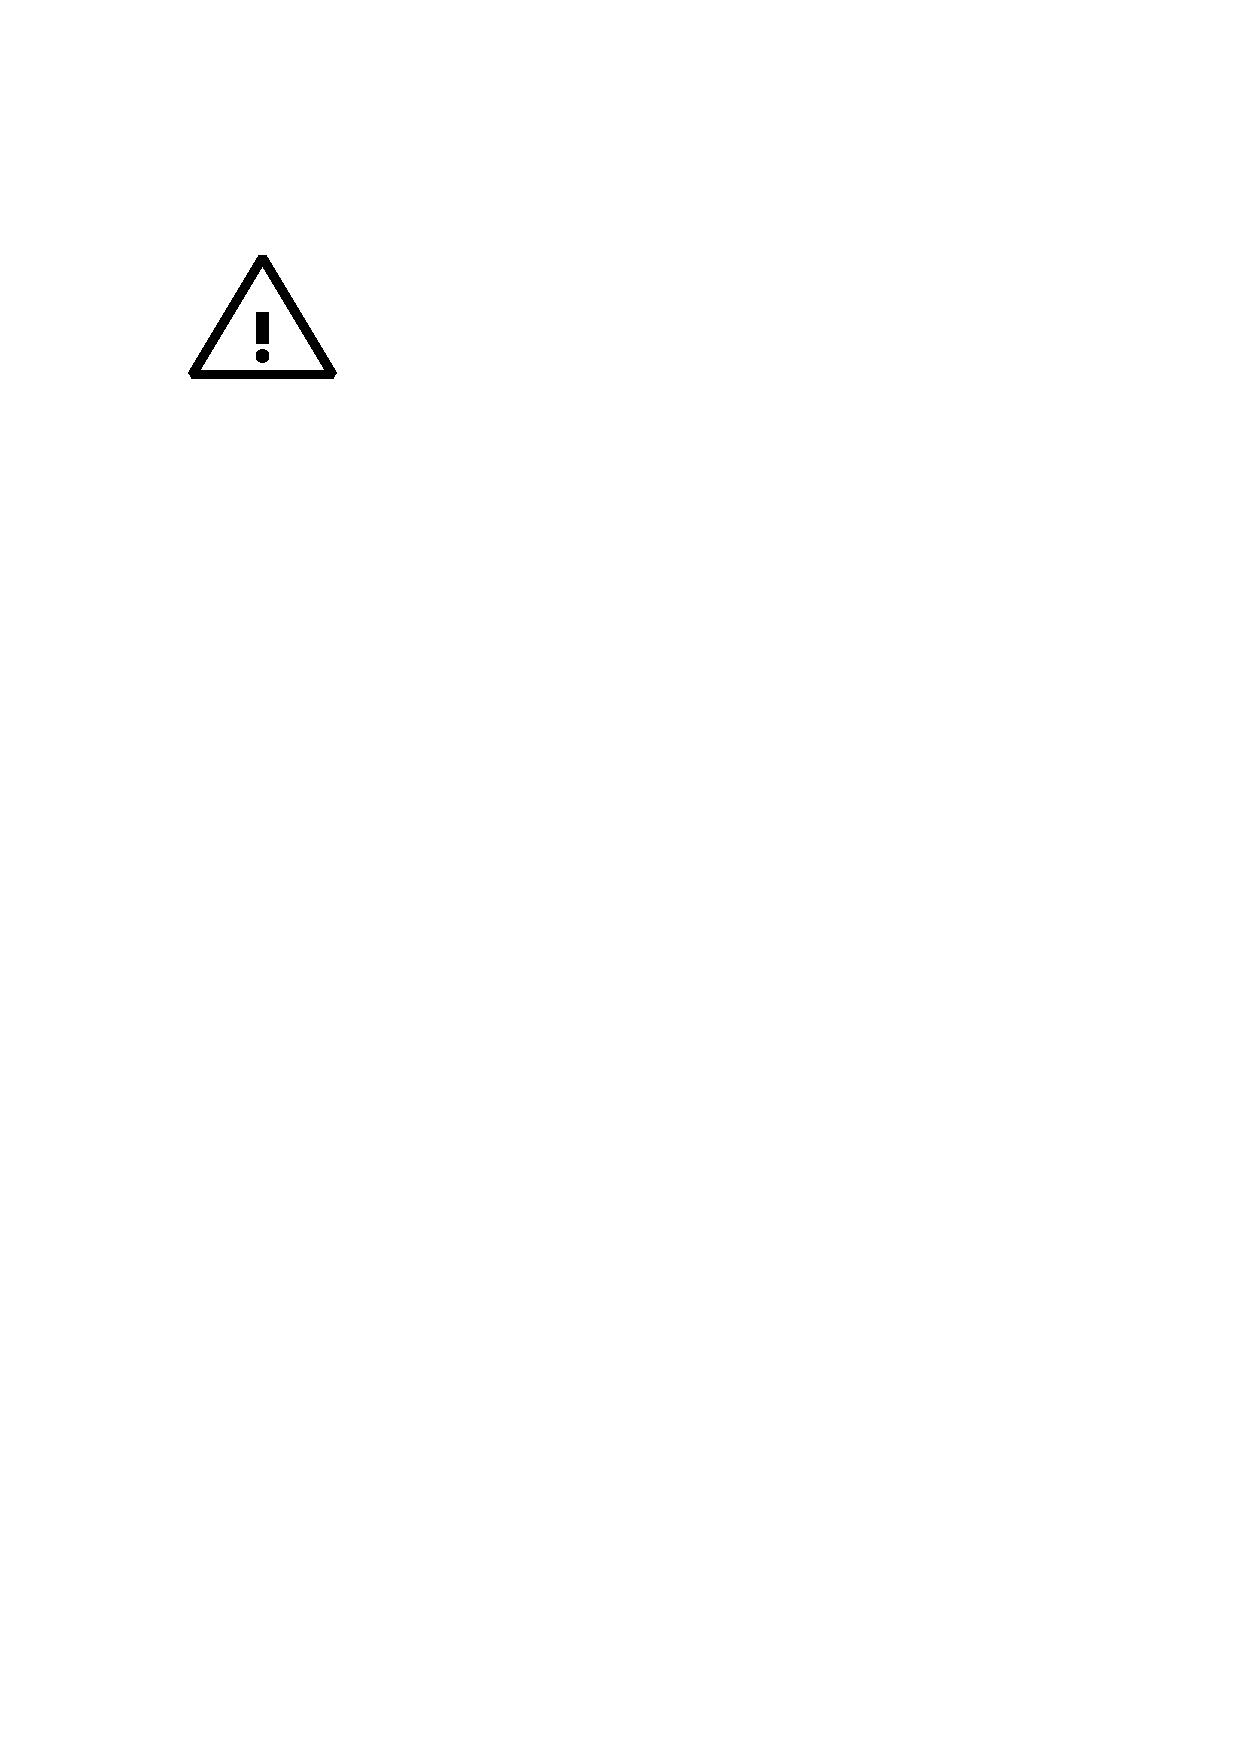
\includegraphics[scale=0.3]{figures/warning}}

\newcommand{\future}[1]{
\noindent\begin{tabular}{|c|}
\colorbox[gray]{0.85}{
  \begin{minipage}{149mm}
  \begin{center}
  {\bf{}Future work}
  \end{center}
  \end{minipage}
}\\
{\begin{minipage}{149mm}
 \textit{#1}
 \end{minipage}
} \\
\colorbox[gray]{0.85}{
  \begin{minipage}{149mm}
  ~~
  \end{minipage}
} \\
\end{tabular}
}

\newcommand{\fr}[1]{
  \if \frenchversion 1
    \if \englishversion 1    
    \vspace{2mm}
    \noindent\begin{tabular}{|c}
      {
        \begin{minipage}{15.5cm}
          \textit{#1}
        \end{minipage}
      }
    \end{tabular}
    \else
    #1
    \fi
  \fi
}

\newcommand{\en}[1]
{
  \if \englishversion 1
  #1
  \fi
}

\newcommand{\sectionenfr}[2]
{
  \if \frenchversion 1
    \if \englishversion 1    
     \section{#1 / \textit{#2}}
    \else
      \section{#2}
    \fi
  \else
    \section{#1}
  \fi
}

\newcommand{\subsectionenfr}[2]
{
  \if \frenchversion 1
    \if \englishversion 1    
     \subsection{#1 / \textit{#2}}
    \else
      \subsection{#2}
    \fi
  \else
    \subsection{#1}
  \fi
}

\newcommand{\subsubsectionenfr}[2]
{
  \if \frenchversion 1
    \if \englishversion 1    
     \subsubsection{#1 / \textit{#2}}
    \else
      \subsubsection{#2}
    \fi
  \else
    \subsubsection{#1}
  \fi
}

\newcommand{\chapterenfr}[2]
{
  \if \frenchversion 1
    \if \englishversion 1    
     \chapter{#1 / \textit{#2}}
    \else
      \chapter{#2}
    \fi
  \else
    \chapter{#1}
  \fi
}

\makeindex

%\pagestyle{empty}

\begin{document}
%==================== COUVERTURE =========================
\thispagestyle{empty}

\noindent\hrulefill\\

\noindent
\hfill
\includegraphics[scale=0.20]{figures/logo_unistra}

\noindent\hrulefill\\

\begin{center}

\vskip 5mm
\Huge{\bf{}Programmer's Reference Manual}
\\
\vskip 5mm

\includegraphics[scale=2.0]{figures/lisaac}
\\
\vskip 10mm
\Huge{\bf{}Lisaac V.0.4}
\\
\vskip 15mm
\Large{\it{}The power of simplicity at work for You}
\\
\vskip 10mm
\noindent\hrulefill\\
\vskip 4mm
S{\sc{}onntag} Beno\^\i t ({\tt{}benoit.sonntag@lisaac.org})\\

\end{center}  

%\vskip 1mm
\noindent\hrulefill\\

\newpage
\thispagestyle{empty}

%\vskip 200mm

\begin{center}
\Large{\bf{}Document history}

\vskip 10mm
\begin{tabular}{l l}
{Version 0.1} & {September 12, 2003}\\
{}            & {Benoit Sonntag, Dominique Colnet,} \\
{}            & {Olivier Zendra, Jerome Boutet}\\
{} & {} \\
{Version 0.2} & {October 20, 2004}\\
{}            & {Benoit Sonntag, Jerome Boutet}\\
{} & {} \\
{Version 0.3} & {September 24, 2007} \\
{}            & {Benoit Sonntag, Alexandre Chabert}\\
{} & {} \\
{Version 0.31} & {September 22, 2008} \\
{}            & {Benoit Sonntag, Pierre-Alexandre Voye}\\
{} & {} \\
{Version 0.4} & {\today} \\
{}            & {Benoit Sonntag}\\
\end{tabular}
\end{center}

\newpage
\setcounter{page}{1}
\tableofcontents
%*********************************************************
\chapterenfr{Introduction}{Introduction}
\label{introduction}
%*********************************************************
%
\en{
Lisaac is the first object-oriented language based on prototype
concepts really compiled, with system programming facilities.  
Two languages are at its origin:
the Self language \cite{ungar87b} for its flexibility and the concept
of dynamic inheritance as well as the  
Eiffel language \cite{meyer94a} \index{Eiffel} for its static typing
and security (programming by contract). 
The Lisaac compiler produces optimized Ansi C code later compilable on
any architecture equipped with an appropriate C Compiler (GCC or
others), thus making Lisaac a truly multi-platform language. 
Moreover, performance results of compiled objects show that it is possible to
obtain executables from a high-level prototype-based language that are
as fast as C programs.
}

\fr{
Lisaac est le premier langage objet bas\'e sur le concept des prototype
\`a \^etre r\'eellement compil\'e, tout en \'etant muni de facilit\'es pour la
programmation syst\`eme.  
Celui-ci trouve son origine dans deux langages :
Le langage Self \cite{ungar87b} pour sa flexibilit\'e et le concept
d'h\'eritage dynamique, ainsi que le langage Eiffel pour le typage
statique et la programmation par contrat. 
Le compilateur Lisaac produit un code Ainsi C optimis\'e compilable sur
toute architecture suportant un compilateur C (GCC ou autre), faisant
de Lisaac un langage r\'eellement multiplateforme.
Les performances obtenu avec la compilation d'objet d\'emontre qu'il est
possible d'obtenir un binaire aussi rapide que du C, m\^eme avec un
langage objet \`a prototype. 
}

\future{
Voici le futur !!!\\
Welcome to the future\\
in the Matrix !
}

%=========================================================
\sectionenfr{Motivation}{Avant propos}
\label{introduction:motivation}
%=========================================================
%
\en{
The design as well as the implementation of the \isaac
\footnote{Isaac:Object-oriented Operating System.} operating system
\cite{httpisaac} led us to design a new programming language 
named Lisaac.

Lisaac integrates communications protection mechanisms, system
interruptions support as well as drivers memory mapping. 
The use of prototypes and especially dynamic inheritance fits perfectly
the construction of a flexible operating system.

The purpose of our project is to break from the internal rigidity of
current operating systems architecture that mainly
depends, in our opinion, on the low-level languages that have been
used to write them.\\ 
Thus, Isaac has been fully written in a high-level
prototype-based language.\\

The evolution of programming currently fulfills
nowadays data-processing needs and constraints in terms of 
software conception and production.\\
Nevertheless, modern languages such as object-oriented ones have
never brought a real alternative to their procedural counterparts
like C  in the development of modern operating systems.\\

Historically, during the creation of an OS, 
programming constraints related to the hardware have been 
systematically fulfilled with a low-level language, such as C.\\
This choice leads generally to a lack of flexibility that can be 
felt at the applicative layer.\\

Our thoughts led us to design and implement a new object-oriented
language equipped with extra facilities useful for the implementation of an
operating  system.\\
In order to achieve that goal, we started to look for an existing 
object-oriented language with powerful characteristics in terms of 
flexibility and expressiveness.\\

Lisaac also comes from an experiment in the creation of
an operating system based on dynamic objects, which possibilities 
are a subtle mix of Self and Eiffel, with the addition of some
low-level  capabilities of the C language.\\
Our language is the first compiled prototype-based language
really usable. Compiled objects remain objects with all their
capabilities and expressivity preserved. Hardware facilities
are included natively, such as mapping or
interrupt management. 
}

\fr{La conception du syst\`eme
d'exploitation \isaac \footnote{Isaac:Object-oriented Operating
System.} nous a men\'e \`a la conception d'un nouveau langage nomm\'e
Lisaac. 
Lisaac int\`egre des m\'ecanismes de protections de communications, de
support des interruptions, de m\^eme que le mappage en m\'emoire de
donn\'ees pour les pilots de p\'eriph\'eriques. 
L'objectif de notre projet est de se d\'epartir de la rigidit\'e interne
des syst\`emes d'exploitations d\'ependant principalement, selon nous, des
langages bas niveau utilis\'es pour les \'ecrire.
Ainsi, Isaac a \'et\'e int\'egralement \'ecrit avec un langage haut niveau;
\\
L'\'evolution du march\'e du logiciel et de la technologie implique de
nouvelles contraintes en terme de conception 
et de d\'eveloppement qui implique d'utiliser des langages de haut niveau.
Malgr\'e cet \'etat de fait, les syst\`emes d'exploitations n'ont pour le
moment d'autres alternative que d'\^etre \'ecris dans des langages
proc\'eduraux comme C.
\\
Ces choix et contraintes impliquent un manque patent de
flexibilit\'e qui peut seulement \^etre atteint au niveau applicatif.
Notre conception de la probl\'ematique nous a conduit \`a impl\'ementer
un nouveau langage objet flexible, expressif et puissant, 
muni de facilit\'es permettant la programmation syst\`eme.
Lisaac est ainsi le fruit d'un marriage subtil entre Self et Eiffel,
adjoint de facilit\'es syst\`emes. 
Les objets compil\'es restent ainsi des objets conservant toutes leurs
capacit\'es et expressivit\'e. 
}

%=========================================================
\sectionenfr{The Lisaac compiler}{Le compilateur Lisaac}
\label{introduction:compiler}
%=========================================================
%
\en{The Lisaac compiler produces optimized C Ansi Code, which can then be
compiled on every architecture with an appropriate C Compiler (GCC or others).\\

The compiler is fully written in Lisaac, the boostrap having been done in 2004, january.

The bootstrap mechanism is explained in the following figure.

State 1: the first version of the Lisaac compiler is written in
another language (here Eiffel), and compiled as every other Eiffel
code with the Eiffel Compiler. 
It produces an executable, the first version of Lisaac compiler.

State 2: the source code of the first compiler is fully translated in Lisaac.
We then use our compiled Lisaac compiler version 1 to compile the new code
(as we can do for every program written in Lisaac). It produces an executable,
the second version of Lisaac compiler. In fact, if there is no error,
version 1 and version 2 operate equally, the only difference being the Eiffel
dependance for the first one.

State 3: the source code of the compiler version 2, written entirely in Lisaac,
is compiled again, this time using the version 2 of our Lisaac
compiler. It produces the version 3 of the Lisaac compiler.

Every iteration of the state 3 doesn't change the produced executable,
we are in a stable state. 
Of course, the code of the compiler has to be error free before
starting the bootstraping operation. 
The advantage of this boostrap is that we are now totally independent
of another language: the compiler is now written in Lisaac, with a
usable version compiled with itself: the compiler is built using only
Lisaac technology.
}

\fr{
Le compilateur Lisaac produit du code C optimis\'e compilable sur toutes les architectures proposant un compilateur C (GCC ou autres).
Le compilateur est totalement \'ecrit en Lisaac, le boostrap ayant eu lieu en janvier 2004.
\\
Le bootstrap se d\'eroule de la mni\`ere suivante :
\\
Etape 1 : La premi\`ere version du compilateur Lisaac est \'ecrit dans un autre langage (ici Eiffel, langage objet à classe choisi 
pour sa puissance, sa g\'en\'ericit\'e, l'impl\'ementation native des contrats) et compil\'e comme tout programme Eiffel 
par le compilateur SmartEiffel.
	Il produit un ex\'ecutable, devenant le premier compilateur Lisaac.
\\
Etape 2 : Le code source du premier compilateur est totalement traduit en Lisaac. Nous utilisons ensuite notre compilateur (issu de l'\'etape 1) lisaac
pour compiler le nouveau code (comme nous pouvons le faire avec tout programme \'ecrit en Lisaac).
Cela produit un ex\'ecutable, la seconde version du compilateur Lisaac. S'il  n'y a pas d'erreur,
la version 1 et 2 fonctionnent de la m\^eme mani\`ere, la seul diff\'erence \'etant que le premier est \'ecrit en Eiffel.
\\
Etape 3 : Le code source du compilateur de l'\'etape 2, totalement \'ecrit en Lisaac est compil\'e une nouvelle fois, 
cette fois en utilisant la 2\`eme version du compilateur. Cela produit la 3\`eme version du compilateur. 
\\
Chaque it\'eration de l'\'etape 3 ne change pas l'ex\'ecutable produit\,: nous sommes dans un \'etat stable.
Bien \'evidemment, le code du compilateur doit \^etre exempt d'erreur avant de d'emarrer l'op\'eration de bootstraping.
L'avantage de cette op\'eration de bootstrap est de nous permettre d'\^etre totalement ind\'ependant d'un autre langage\,: 
le compilateur est maintenant \'ecrit en Lisaac, avec une version compil\'e par lui m\^eme.
Le compilateur est ainsi produit en utilisant la technologie Lisaac.
}




\begin{center}
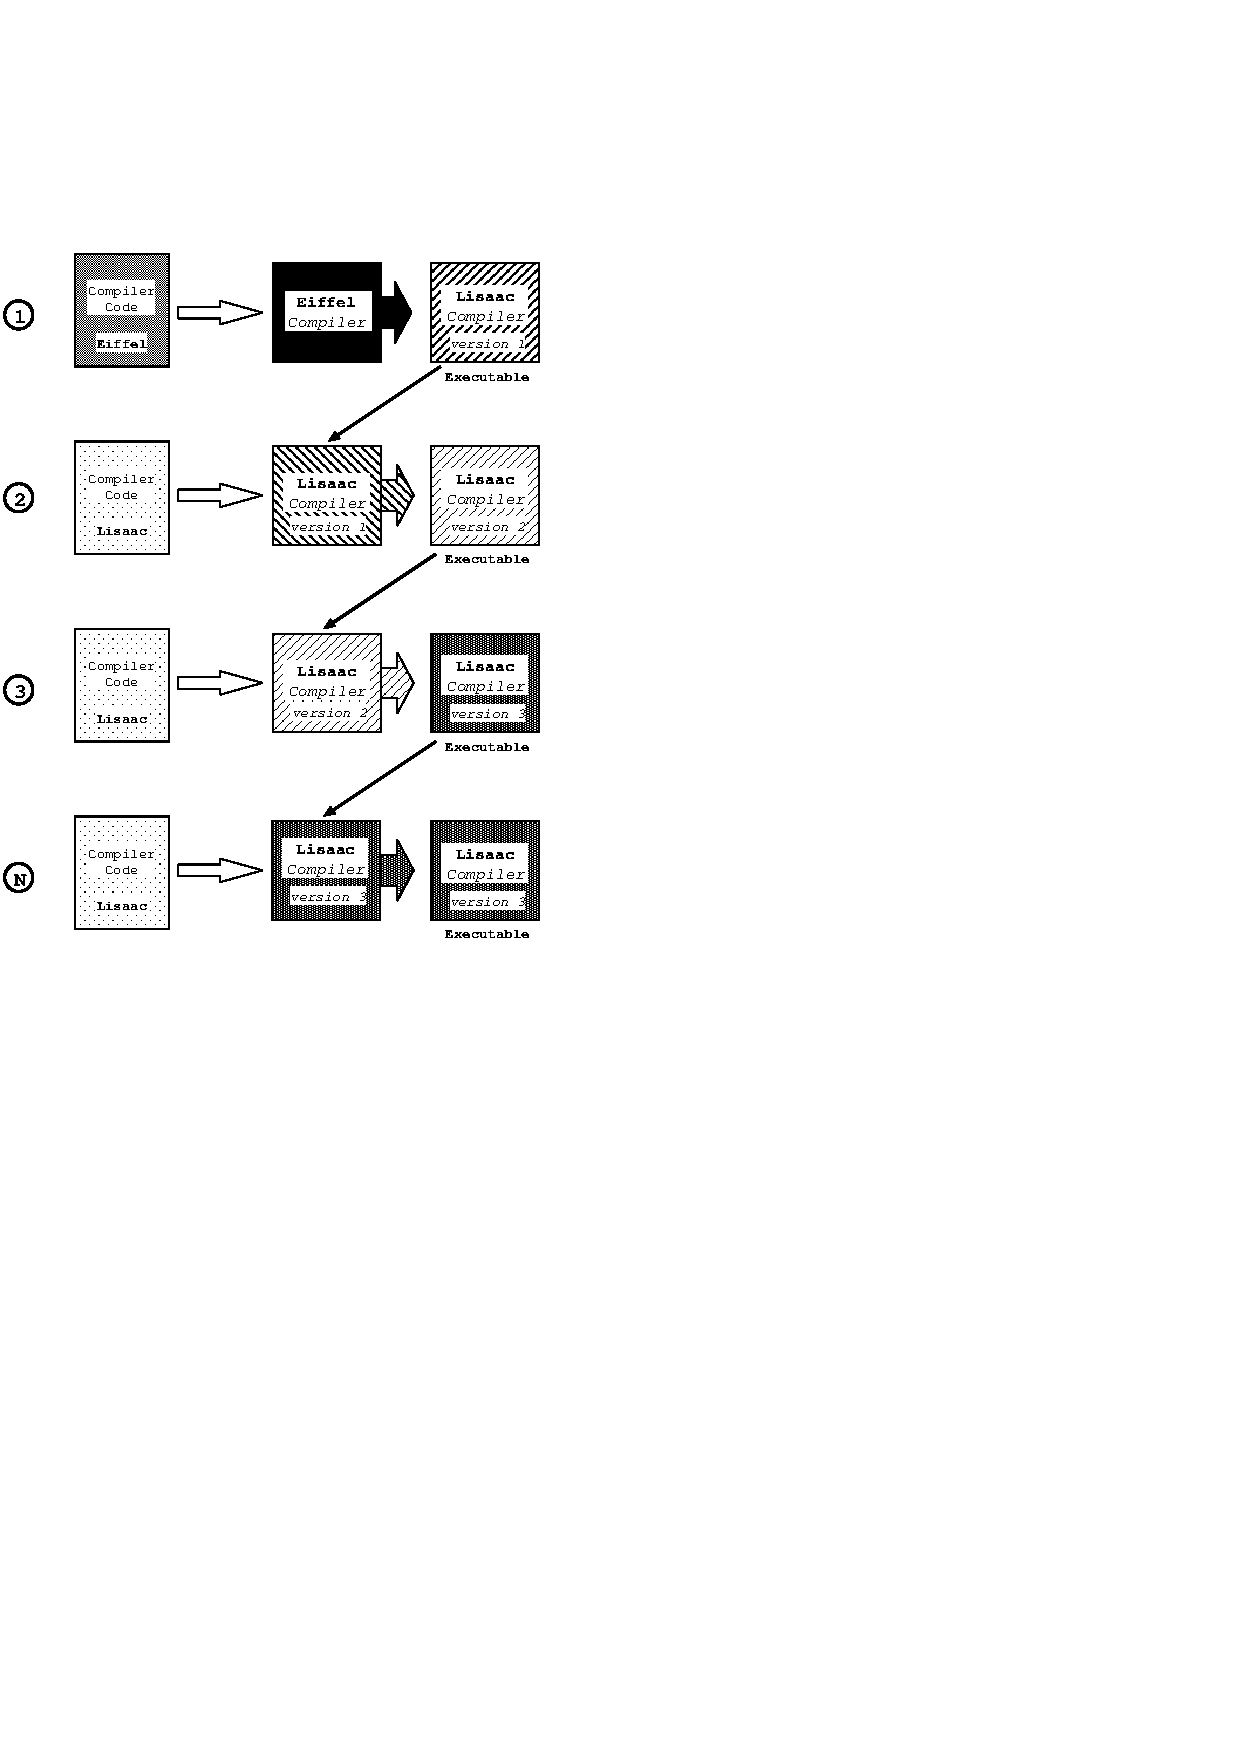
\includegraphics[scale=0.8]{figures/bootstrap}
\end{center}

\en{The compiler can be run on every architecture which have a C compiler.}

\fr{Le compilateur peut \^etre utilis\'e sur toute architecture poss\'edant un compilateur C}
\begin{center}
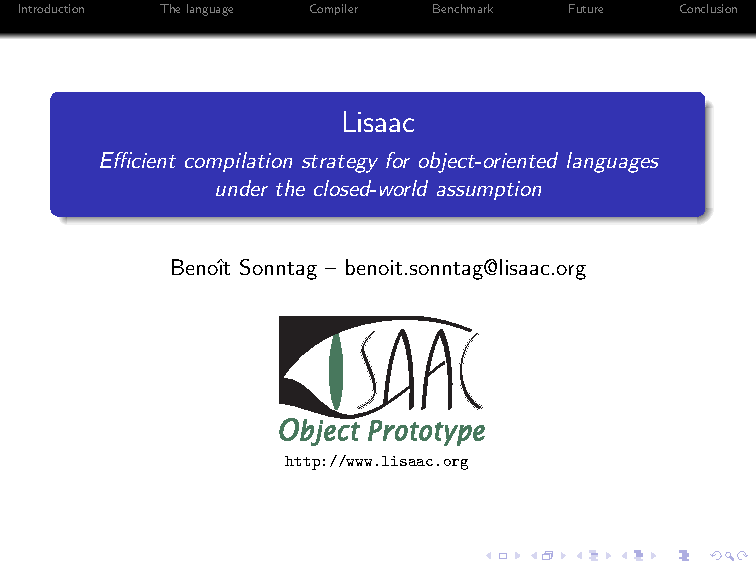
\includegraphics[scale=0.8]{figures/compiler}
\end{center}

%=========================================================
\section{Why Using Lisaac}
\label{introduction:use_of_lisaac}
%=========================================================
%
\en{Lisaac was first developped to implement the \isaac Operating System but
became an independent object oriented language, perfectly usable to
write all kind of programs.\\

It has numerous advantages: it's a powerful high level
language, based on prototype concepts. Security has been a real aspect 
from the start, with the static typing and
assertion management (programming by contract) such as
{\it{}Requires}, {\it{}Ensures} and {\it{}Invariant}, and lots of
verifications during compilation.\\

Many high-level optimizations also provide efficiency and speed to the compiled code.\\

A large library, fully written in Lisaac, supply the programmer with
a large scale of built-in prototypes and functions, such as:
\begin{itemize}
	\item{Number (signed / unsigned 8, 16, 32, 64 bits integer; real (fixed or float); infinite accuracy integer)}
	\item{Collections: variable arrays, linked-lists, dictionary (associativity key-value), set}
	\item{Hash coding}
	\item{Memory management}
	\item{Input / Output}
	\item{File System (Unix / Linux ; Windows / Dos)}
	\item{Image format (bitmap; vectorial)}
	\item{Graphic (8, 15, 16, 24, 32 bits)}
	\item{Time and Date}
\end{itemize} 
}

\fr{
	Lisaac a \'et\'e avant tout impl\'ement\'e pour d\'evelopper le syst\`eme d'exploitation Isaac, mais devenant par la suite un langage g\'en\'eraliste.
\\
	Il a de nombreux avantages\,: C'est un langage haut niveau tr\`es puissant, bas\'e sur les concepts à prototypes.
	La s\'ecurit\'e logiciel fut un aspect pris en compte d\`es le d'epart, avec le typage static et la gestion des contrats comme les
{\it{}Requires}, {\it{}Ensures} and {\it{}Invariant}, ainsi que les nombreuses v\'erifications durant la compilation.
}


%=========================================================
\section{Notations}
\label{introduction:notations}
%=========================================================
%
\en{In this document, you'll find memory representation of objects.
Here is the caption of the figures.
}
\fr{Dans ce document, vous trouverez des figures repr\'esentant la pr\'esence en m\'emoire des objets. La liste des figures sont les suivantes\,:}
\begin{center}
	\includegraphics[scale=1]{figures/caption.ps}
\end{center}

%*********************************************************
\chapter{Quickstart - for beginners}
\label{quickstart}
%*********************************************************
%
\en{After reading this chapter, you will be able to write simple programs.\\
The next chapter will teach you more about Lisaac, allowing you to use all of its capabilities and power.}

\fr{
	Dans ce manuel, vous trouverez de nombreuses repr\'esentations d'objets en m\'emoire. Ici la charte graphique utilis\'ee pour les repr\'esenter.
}
%=========================================================
\section{Lisaac: a prototype based language}
\label{quickstart:prototype_language}
%=========================================================
%
\en{Lisaac is an object oriented language based on prototype concepts.\\
Class and prototype languages differ on few but important points. \index{Class} \index{Prototype}
In a class language, you have to instanciate an object from its description in order to make it alive.\\
In a prototype language, a description of an object is already alive. In Lisaac you can directly use the 
"master" object without having instanciated it. \index{Object}\\
This particular object name is written in capitals and can be used as any other object.\\
Other objects are obtained by cloning the "master" one. The {\bf{}clone} routine is actually not a hard-coded function but one from the library.
\begin{center}
	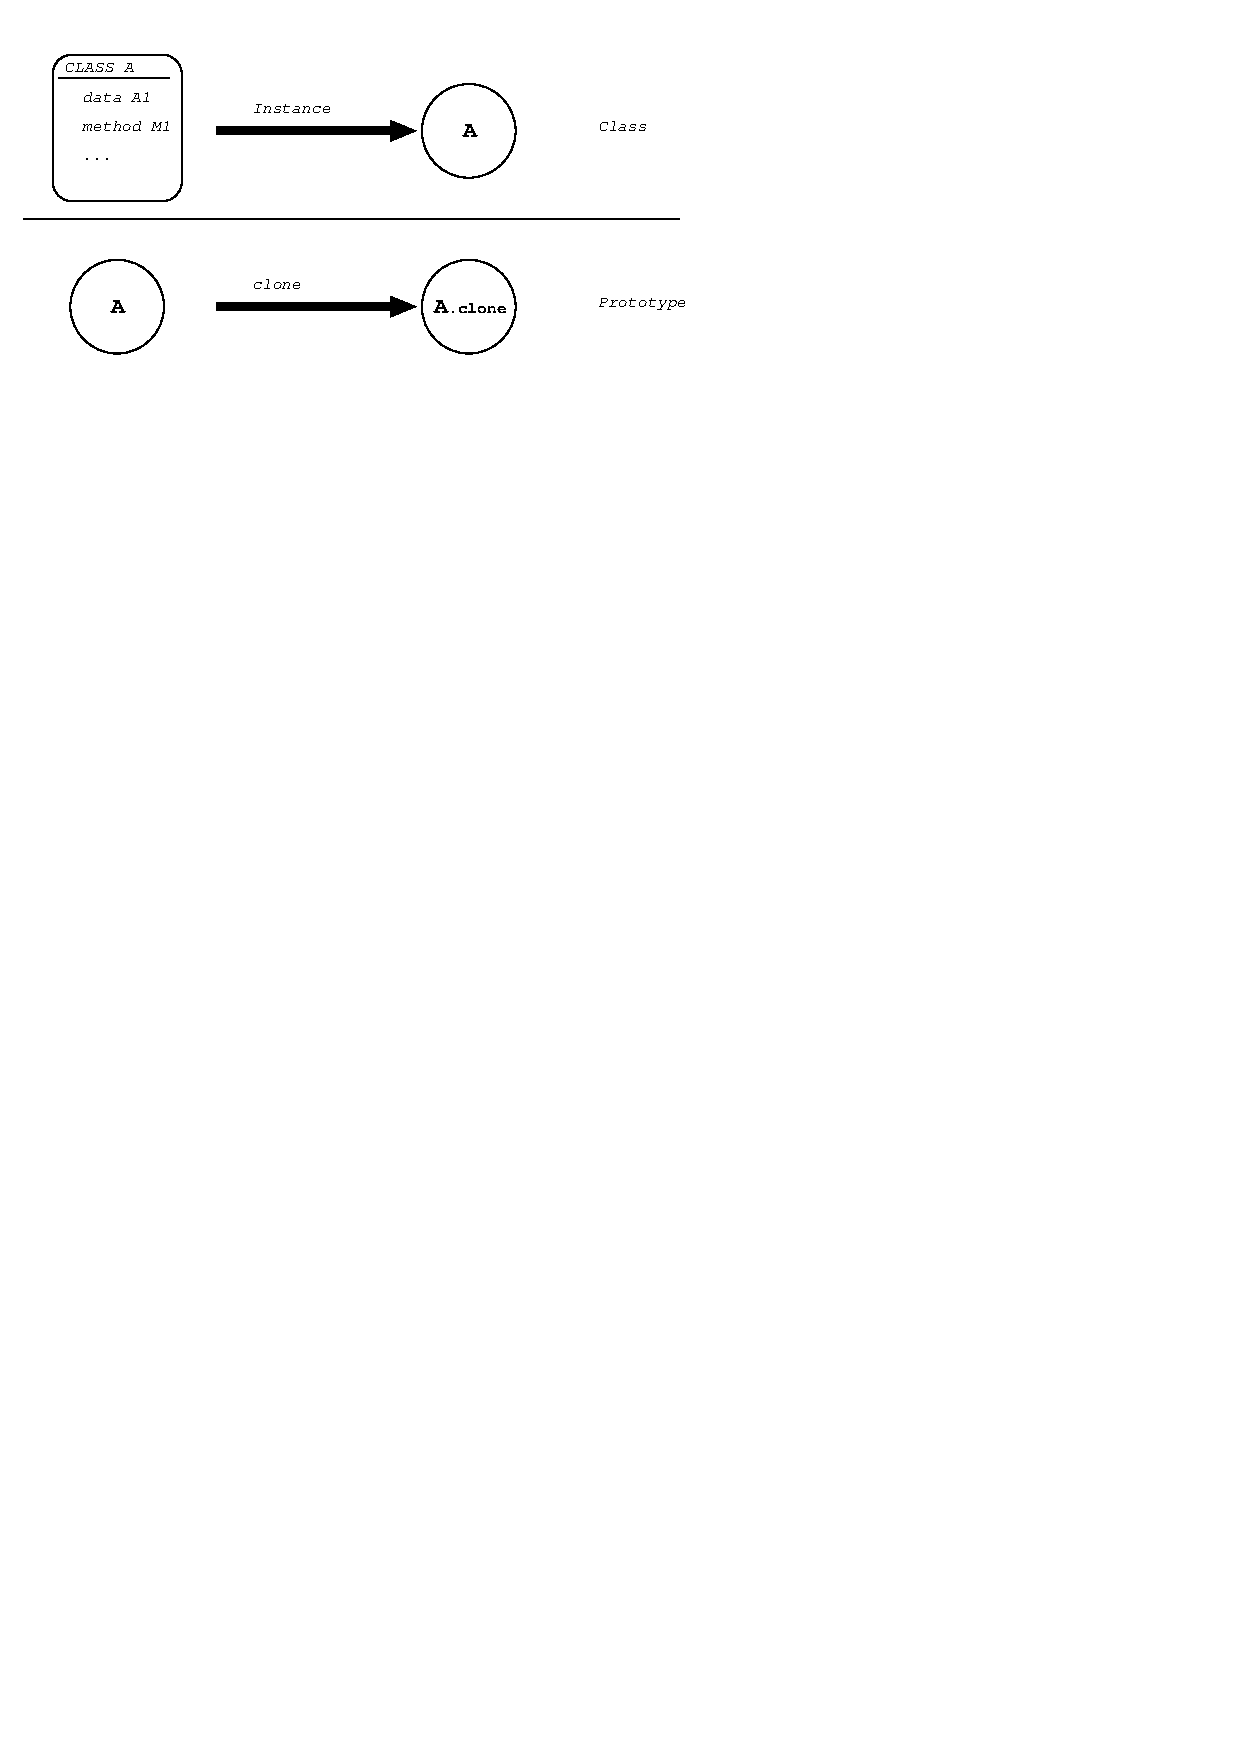
\includegraphics[scale=0.9]{figures/class_vs_prototype1} 
\end{center}
We can see from this property that inheritance is particular. Objects inherit from alive objects, with their own live. 
It permits numerous variations from inheritance, depending of its type ({\bf{} +} or {\bf{} -}), such as sharing parents 
between 2 cloned object, or dynamic inheritance (by changing the reference of the parent). We will see this later.
\begin{center}
	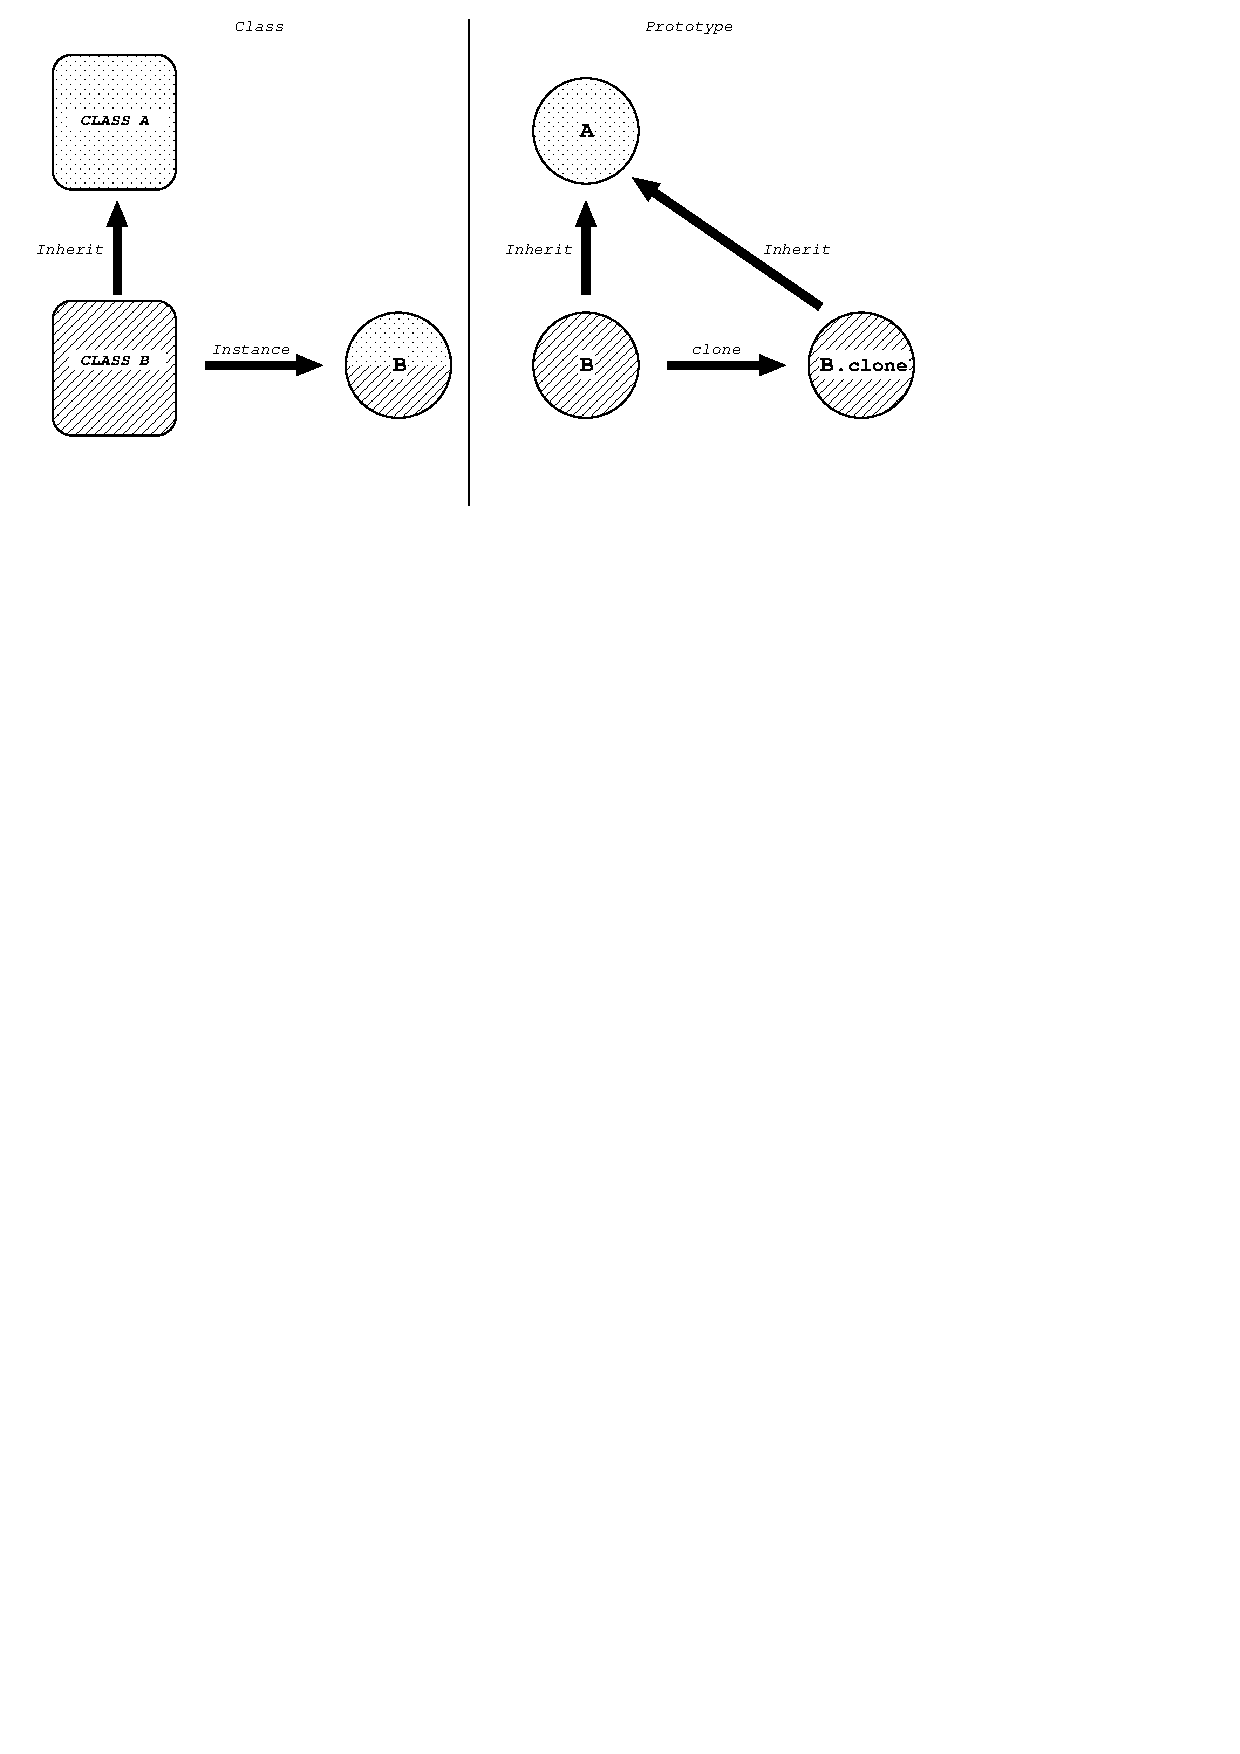
\includegraphics[scale=0.9]{figures/class_vs_prototype2} 
\end{center}
Objects are the fundamental entities in Lisaac; every entity 
in a program is represented by one or more objects. 
Even controls are handled by objects: blocks (\ref{language_reference:blocks} page \pageref{language_reference:blocks}) are 
Lisaac closures used to implement user-defined control structures. 
An object is composed of a set of slots. 
A slot is a name-value pair.
Slots may contain references to other objects. 
When a slot is found during a message lookup (see section \ref{language_reference:section_identifiers:inherit_section:lookup} 
page \pageref{language_reference:section_identifiers:inherit_section:lookup}), the object in the slot is
evaluated.
}

\fr{
Lisaac est un langage objet orient\'e prototype.
Les classes et les prototypes diff\`erent de fa\c con importante sur quelques points.  \index{Class} \index{Prototype}
Dans un langage \`a classe, vous devez instancier un objet \`a partir de sa description pour le rendre vivant.
Dans un langage objet \`a prototype, la description de votre objet est dors et d\'ej\`a vivante.
Dans le langage Lisaac, vous pouvez d\'ej\`a utiliser l'objet "Ma\^\i tre" sans avoir \`a l'instancier. \index{Object}\\
Cet objet particulier est \'ecrit en lettre capitale et peut \^etre utiliser comme d'autres objets.
Les autres objets peuvent \^etre obtenus en clonant l'objet "Ma\^\i tre". 
La m\'ethode {\bf{}clone} n'est pas une primitive du compilateur\,: elle tout simplement d\'efini dans le prototype {\sc{}object}.
		\begin{center}
		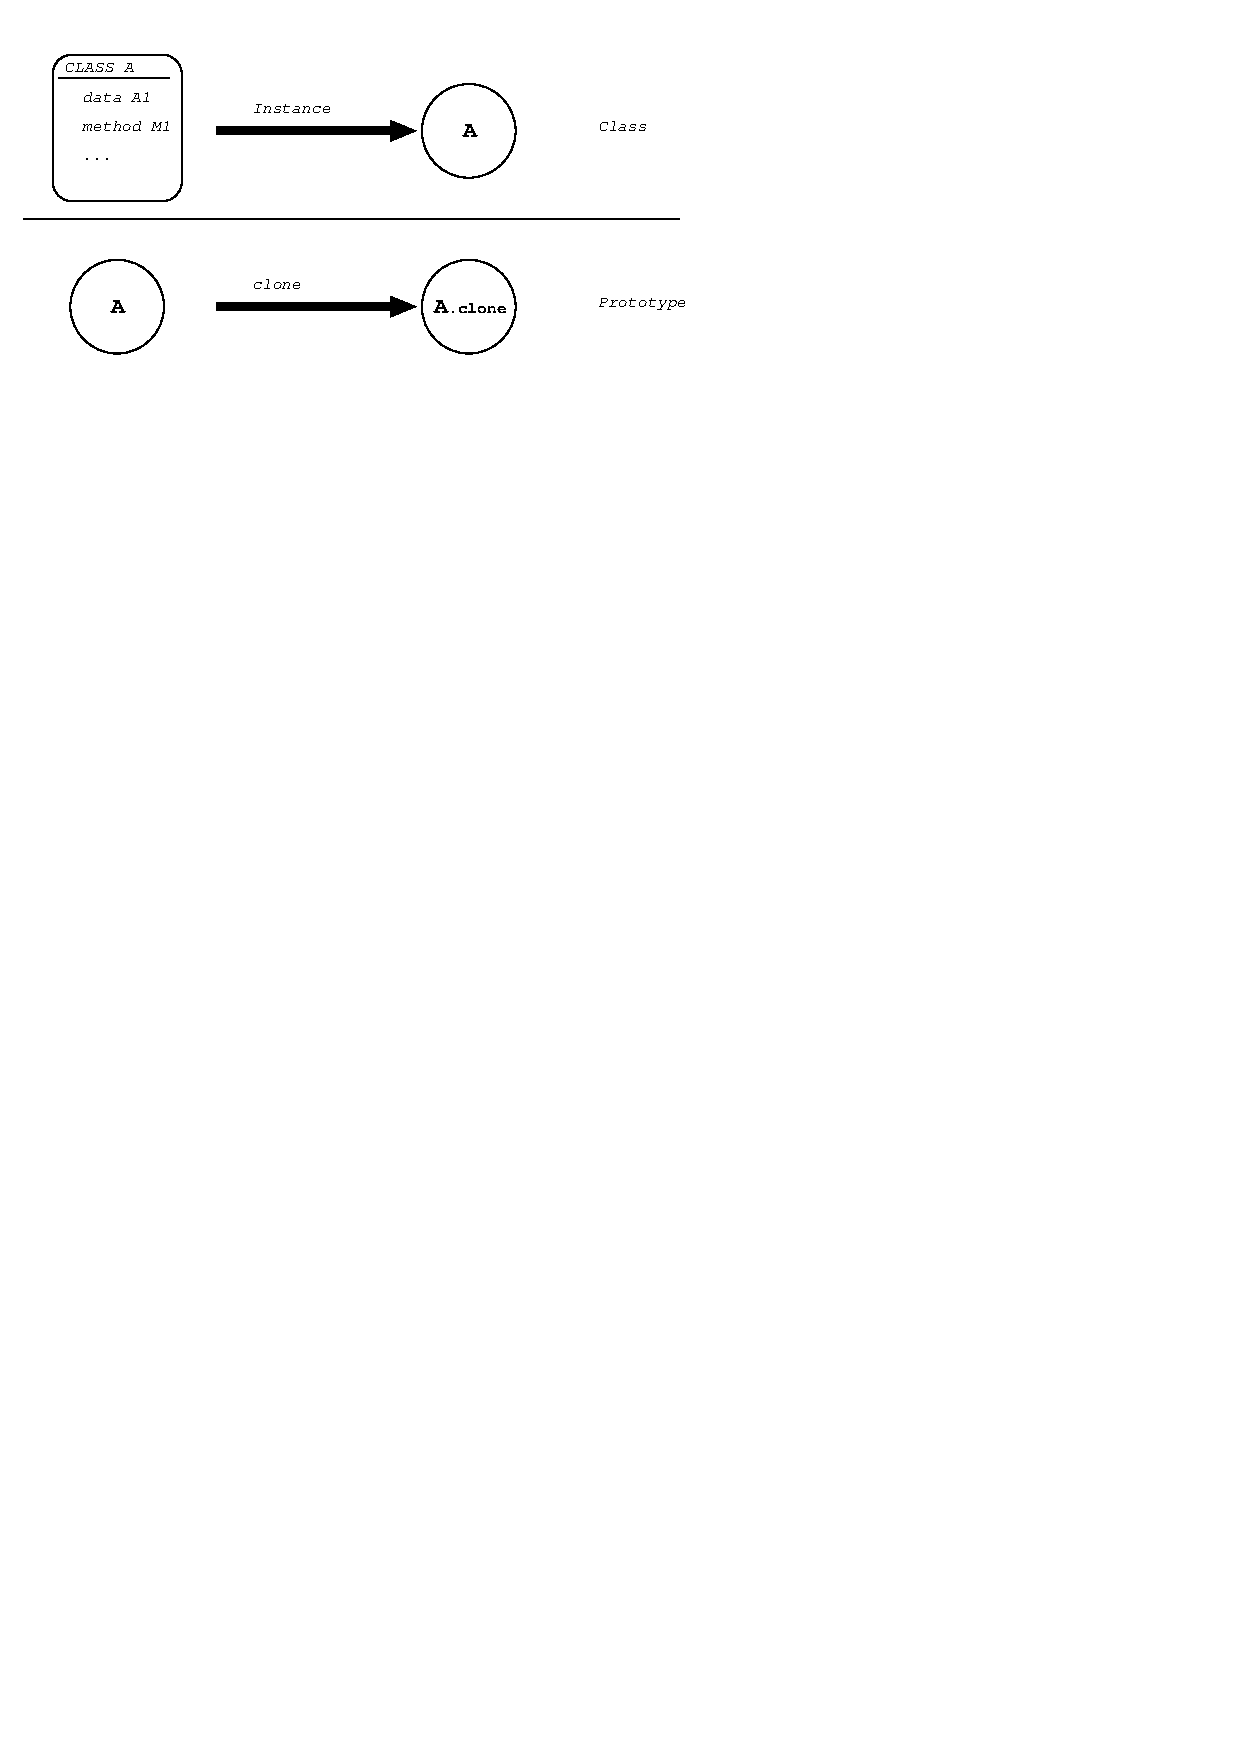
\includegraphics[scale=0.9]{figures/class_vs_prototype1} 
		\end{center}
Nous pouvons voir par ces propri\'et\'es que dans ce mod\`ele, l'h\'eritage est particulier\,: 
 Les objets h\'eritent d'autres objets vivants, qui vivent leur propre vie.
Il est ainsi permis de nombreuses variations, en fonction de son type  ({\bf{} +} ou {\bf{} -}), 
comme partager un parent entre 2 objets clon\'es, ou l'h\'eritage dynamique (en changeant la r\'ef\'erence au parent). 
Nous verrons tout cela plus tard.
			\begin{center}
			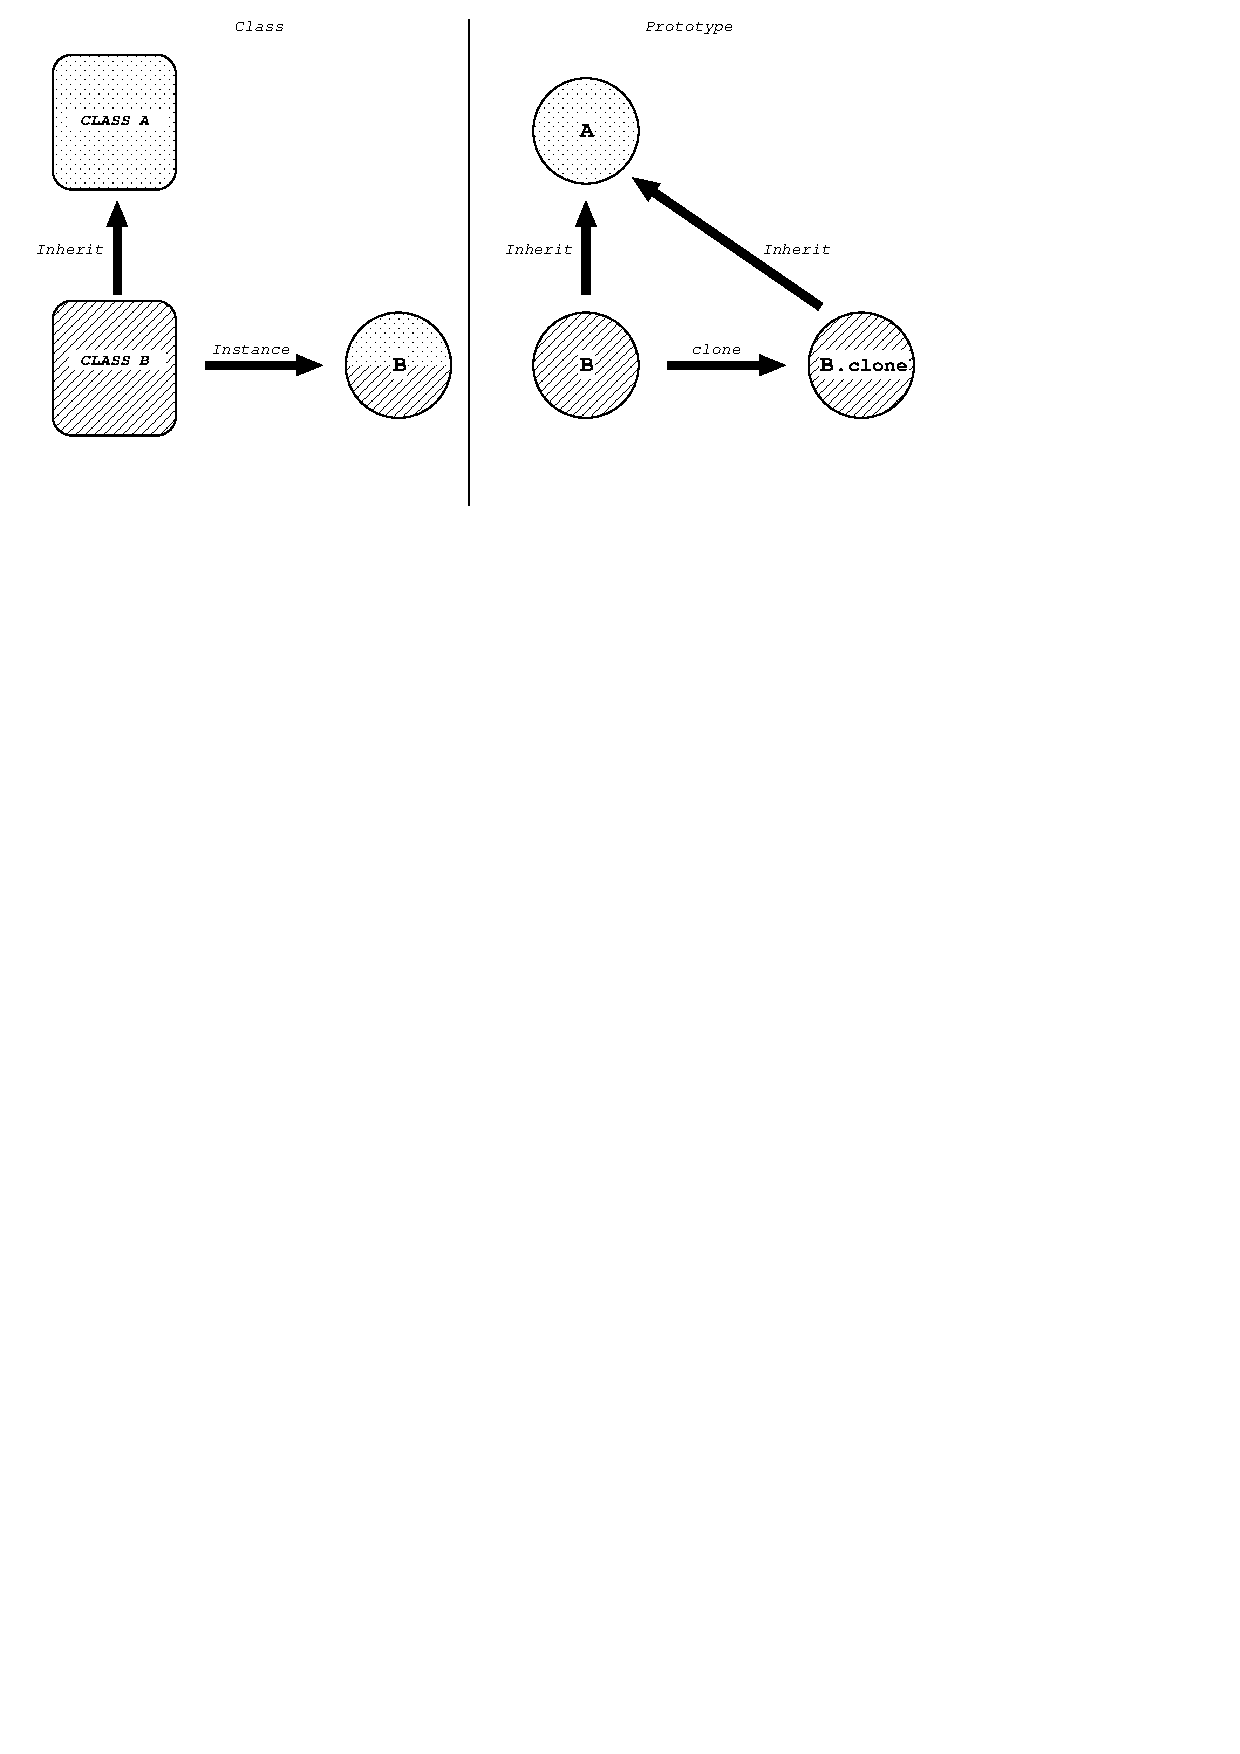
\includegraphics[scale=0.9]{figures/class_vs_prototype2} 
			\end{center}
L'objet est l'entit\'e fondamentale en Lisaac : toute entit\'e est un programme repr\'esent\'e par un ou plusieurs objets.
Toutes les structures de contr\^ole sont prise en main par des objets : les blocks (\ref{language_reference:blocks} page \pageref{language_reference:blocks}) sont en lisaac les fermetures utilis\'ees pour impl\'ementer les structures de contr\^oles.
Un objet est constitu\'e d'un ensemble de slots
Un slot est une paire nom-valeur.
Les slots peuvent contenir des r\'ef\'erences \`a d'autres objets
Quand un slot est trouv\'e durant un lookup de message (voir la section \ref{language_reference:section_identifiers:inherit_section:lookup}
page \pageref{language_reference:section_identifiers:inherit_section:lookup}), l'objet du slot est \'evalu\'e.
}


%=========================================================
\section{Notations}
\label{quickstart:notations}
%=========================================================
%
\en{Lisaac is case sensitive, and respects the following constraints:\\
Variables and slots are written with small letters ({\it{}x},{\it{}counter},\ldots).\\
Type of objects (or "master" name object / prototype) are in capital letters ({\sc{}integer},{\sc{}boolean},\ldots).\\
Keywords are written in small letters but start with a capital letter ({\bf{}Section},Header,\ldots).\\

Symbol {\bf{} :=} is an affectation. Be careful not to use symbol {\bf{} =} which compares 2 objects and returns a boolean.\\
You will see symbol {\bf{} +} or {\bf{} -} before the slots. It defines the type of the slot and is mandatory. Its role will be explained in the following pages.\\

A sequence ends with {\bf{} ;} .If not, the compiler continues to the following line.\\
You can define a list of sequence between {\bf{} (} and {\bf{} )}.
See section \ref{language_reference:lists} on page \pageref{language_reference:lists} for more information on instruction lists.

Comments begin with {\bf{} //} and stop at the end of the line.\\
Multi-lines comments start with {\bf{} /*} and end at {\bf{} */}.
}

\fr{
Lisaac est sensible \`a la casse et respecte les contraintes suivantes\,:
Variables et slots sont \'ecrit en minuscule ({\it{}x},{\it{}counter},\ldots).\\
Type et objets (ou le nom de l'objet/prototype "Ma\^\i tre") sont en lettres majuscules ({\sc{}integer},{\sc{}boolean},\ldots).\\
Mot-cl\'es sont \'ecrit en lettre minuscule, la premi\`ere lettre \'etant en majuscule  ({\bf{}Section},Header,\ldots).\\
\\
Le symbole {\bf{} :=} est une affectation. Faites bien attention \`a ne pas utiliser le symbole {\bf{} =} qui compare deux objets et retourne un bool\'een.\\
Vous verrez le symbole  {\bf{} +} or {\bf{} -} avant chaque slot. Il d\'efinie le type, la port\'ee du slot et est obligatoire. 
Son r\^ole sera expliqu\'e dans les prochains pages.
}

%=========================================================
\section{Objects}
\label{quickstart:objects}
%=========================================================
%
\index{Object}
\en{
In Lisaac, objects are the fundamental entities. Everything is represented by one or more of them, 
from a simple Integer or Boolean to more complex entities like arrays or windows.\\
An object is written in one and only one file, named as the name of the object and followed by the extension {\bf{} .li} .\\
For example, {\tt{}integer.li}, {\tt{}boolean.li},{\tt{}window.li}, \ldots\\

The source code of an object is divided in sections.\\
{\bf{}Section Header} is needed. In this section, you define the name of the object. 
Then you have the {\bf{}Section Public}, in which you define the slot which will be 
executed at initialization (more in later sections).\\

{\bf{}Section},  {\bf{}Header} and  {\bf{}Public} are keywords.\\

{\it{}Example}: file {\tt{}hello\_world.li}
{\tt\begin{tabbing}
{\bf{}Section Header}\\
~~\=+ {\bf{}name}~~~~~\=:= {\sc{}hello\_world};~~~\=// Name is in capital letters \\
{\bf{}Section Public}\\
  \>/* \ldots */\\
\end{tabbing}}

\warning{} Note that there is no {\bf{} ;} after {\bf{}Section xxxx} .
}

\fr{
En lisaac, l'entit\'e fondamentale est l'objet. Toutes les entit\'es du language sont 
constitu\'es de l'un d'entre deux, que ce soit un simple entier ou bool\'een,
ou un objet plus complexe comme une collection ou une fen\^etre.\\
Un objet est d\'ecrit dans un et un seul objet, nomm\'e comme le nom de
l'objet - suivi de l'extention {\bf{} .li} .\\ 
Par exemple, {\tt{}integer.li}, {\tt{}boolean.li},{\tt{}window.li}, \ldots\\
Le code source de l'objet est divis\'e en sections.
La {\bf{}Section Header} est obligatoire. C'est dans cette section que
vous pouvez d\'efinir le nom de l'objet, entre autres choses. 
Vous trouverez ensuite la {\bf{}Section Public}, dans laquelle vous
pouvez d\'efinir le slot qui sera ex\'ecut\'e \`a l'initialisation.\\ 
{\bf{}Section},  {\bf{}Header} et  {\bf{}Public} sont des mots
cl\'es.
}
\fr{
{\it{}Exemple}: le fichier {\tt{}hello\_world.li}
{\tt\begin{tabbing}
{\bf{}Section Header}\\
~~\=+ {\bf{}name}~~~~~\=:= {\sc{}hello\_world};~~~\=// Le nom est toujours en lettres majuscules \\
{\bf{}Section Public}\\
  \>/* \ldots */\\
\end{tabbing}
}
\warning{Notez qu'il n'y a pas de {\bf{} ;} apr\`es {\bf{}Section xxxx}.}
}

%=========================================================
\section{Slots}
\label{quickstart:slots}
%=========================================================
%
\index{Slot}
\en{An object is composed of slots, which are services given by the object.\\
A slot can be data as well as code (function or method).\\
A slot is defined by a name. It can also add a static type for data and functions.\\
A slot is prefixed by the {\bf{} +} or {\bf{} -} sign, which gives its type (to simplify, with {\bf{} -} values are shared between objects while values are local to the object with {\bf{} +} ).\\
The type is defined after the sign {\bf{} :}.

{\tt\begin{tabbing}
{\bf{}Section Header}\\
~~\=+ {\bf{}name}~~~~~\=:= {\sc{}my\_object};~\=// Name is in capital letters \\
{\bf{}Section Public}\\
  \>+ {\bf{}slot}:{\sc{}integer};      \>     \>// Value local to the object, \\
  \>                                   \>     \>// and init with INTEGER default value \\
  \>- {\bf{}slot2}:{\sc{}integer} := 3;\>     \>// Value shared between objects, init with value 3\\
\end{tabbing}}
}
\fr{
Un objet est compos\'e de slots, qui sont autant de serices propos\'es par cet objet.\\
Un slot peut \^etre des donn\'ees autant que du code (fonction ou m\'ethode).\\
Un slot est toujours pr\'efix\'e par le signe {\bf{} +} or {\bf{} -}, qui donne sa port\'ee. 
Pour simplifier, avec {\bf{} -}, les objets sont partag\'es entre objets, tandis qu'avec {\bf{} +}, 
les donn\'ees sont locales \`a l'objet.
Le type est défini après le signe {\bf{} :}.
}

\begin{center}
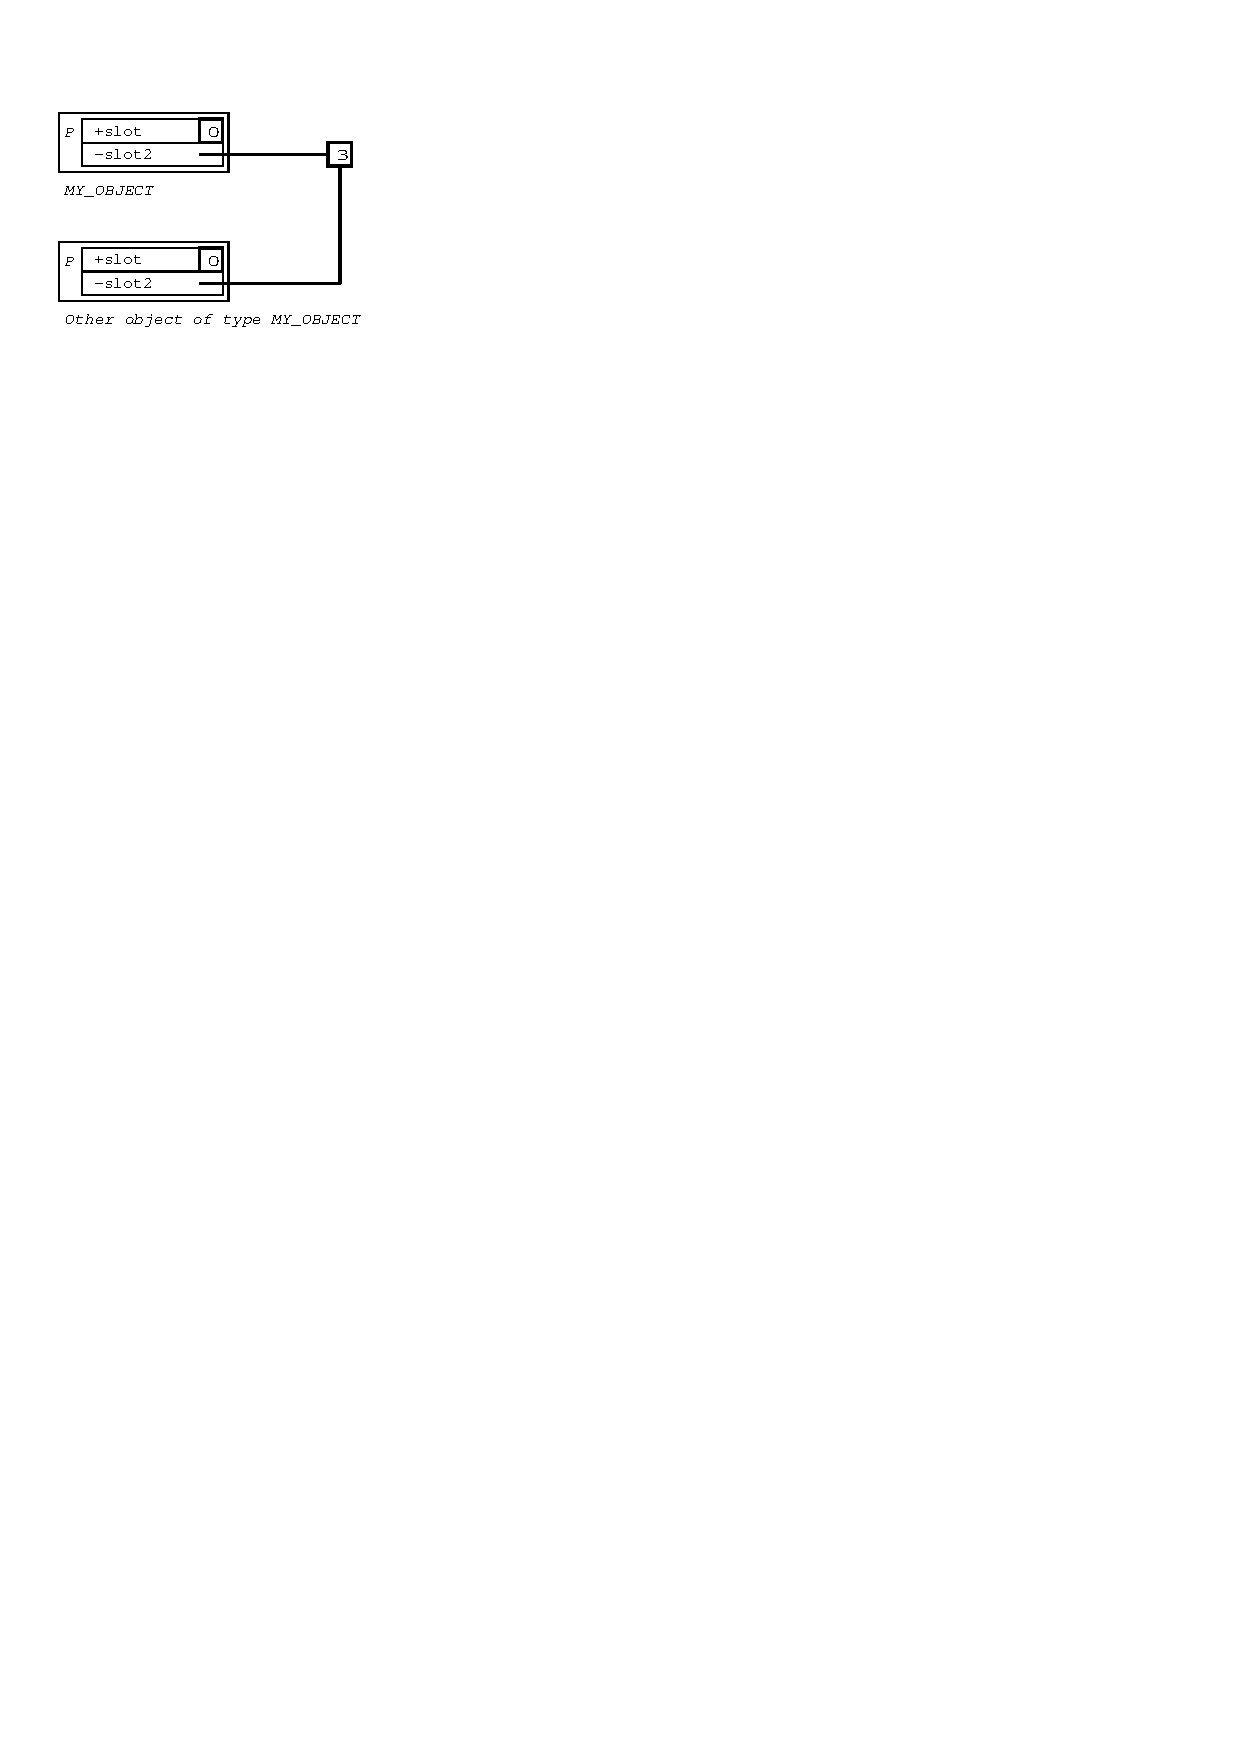
\includegraphics[scale=1.0]{figures/slot_minus_plus}
\end{center}

%---------------------------------------------------------
\subsection{Methods and functions}
\label{quickstart:slots:methods_functions}
%---------------------------------------------------------
%
%---------------------------------------------------------
\subsubsection{Simple slots}
\label{quickstart:slots:methods_functions:simple_slots}
%---------------------------------------------------------
%
\index{Slot, simple}
\fr{
Comme pr\'ec\'edemment d\'efini, un slot peut repr\'esenter une fonction ou une m\'ethode.
Les m\'ethodes (ou routines) sont une notion fondamentales des langages
orient\'e objets, avec le concept connexe qu'est la liaison dynamique
(ou envoi de message, appel de routine, appel de m\'ethode, r\'esolution
dynamique \ldots).\\ 
Il y a deux types de slots. Le premier est ex\'ecut\'e \`a l'initialisation
de l'objet et d\'efini en tant que valeur par d\'efaut d'une variable. 
{\tt\begin{tabbing}
~~\= // L'operation '3 + 4' est evaluee a l'initialisation.\\
  \> + {\bf{}slot}:{\sc{}integer}  := 3 + 4; \\
  \> + {\bf{}slot2}:{\sc{}integer}  := {\bf{}slot} * 2;
\end{tabbing}}
Le second type est ex\'ecut\'e uniquement lors de l''appel du slot, et est
d\'efini par le symbole {\tt <-} symbol. 
{\tt\begin{tabbing}
~~\=+ {\bf{}slot}  :{\sc{}integer}  := 3;\\
  \>// L'operation '5 + slot' est evaluee lors de l'appel de slot2\\
  \>+ {\bf{}slot2} :{\sc{}integer}  <-\\
  \>( 5 + {\bf{}slot} );   
\end{tabbing}}
Un code plus complexe peut bien evidemment être d\'efini entre parenthèses
{\tt\begin{tabbing}
~~\= + {\bf{}slot}  :{\sc{}integer}  := 3;\\
  \> + {\bf{}slot2} :{\sc{}integer}  := 4;\\
  \> + {\bf{}slot3}  <-     // Slot sans valeur de retour\\
  \> (\\
  \>~~\= {\bf{}slot}  := {\bf{}slot} + 3;\\
  \>  \> {\bf{}slot2} := {\bf{}slot} + 5;\\
  \>  \> {\bf{}slot2} := {\bf{}slot2} * 3;\\
  \> );
\end{tabbing}}
Notez que vous pouvez \'ecrire votre code sur une seule ligne, bien que ce soit moins lisible.
La valeur de retour est la dernière valeur, sans {\bf{} ;}.
{\tt\begin{tabbing}
~~\= + {\bf{}slot}  :{\sc{}integer}  := 3; \\
  \> + {\bf{}slot2} :{\sc{}integer}  <-\\
  \> (\\
  \>~~\=slot              // Valeur de retour, evaluee a l'appelle de slot3\\
  \> );\\
  \> + {\bf{}slot3}:{\sc{}integer}  := \\
  \> (\\
  \>  \> {\bf{}slot} := {\bf{}slot} + 6; \\
  \>  \> {\bf{}slot} := {\bf{}slot2} * 5; \\
  \>  \> {\bf{}slot}              // Valeur de retour evaluee lors du chargement de l'objet.\\
  \> ); \\
\end{tabbing}}
\warning{Faites bien attention \`a la coh\'erence du type de l'objet de
retour d\'efini en entête de fonction et le type de l'objet renvoy\'e.\\ 
}
}


\en {
	As said before, a slot can also represent a function or method.\\
	Methods( or routines) are a fundamental notion in object-oriented languages, 
        together with their companion concept late binding (or message sending, 
        routine call, method call, dynamic dispatch, \ldots).\\

	There are two types of code slots. The first one is executed at the load of the object and
	is defined as the default value of a variable.

{\tt\begin{tabbing}
~~\= + {\bf{}slot} :{\sc{}integer}  := 3 + 4;      // Operation '3 + 4' is evaluated at init\\
  \> + {\bf{}slot2}:{\sc{}integer}  := {\bf{}slot} * 2;\\
\end{tabbing}}

	The second type is executed only on the call of the slot and is defined with the {\tt <-} symbol.

{\tt\begin{tabbing}
~~\= + {\bf{}slot}  :{\sc{}integer}  := 3;\\
  \> + {\bf{}slot2} :{\sc{}integer}  <- \\
  \> ( 5 + {\bf{}slot} );   // Operation '5 + slot' evaluated when calling slot2
\end{tabbing}}

	More complex code can be defined within parenthesis.

{\tt\begin{tabbing}
~~\= + {\bf{}slot}  :{\sc{}integer}  := 3;\\
  \> + {\bf{}slot2} :{\sc{}integer}  := 4; \\
  \> + {\bf{}slot3}  <-     // Slot without return value\\
  \> (\\
  \>~~\= {\bf{}slot}  := {\bf{}slot} + 3;\\
  \>  \> {\bf{}slot2} := {\bf{}slot} + 5;\\
  \>  \> {\bf{}slot2} := {\bf{}slot2} * 3;\\
  \> );
\end{tabbing}}

	Note that you can write all your program on the same line, but it's more easy to read to align the code like that.
	The return value of a code is the value of the last code (without {\bf{} ;}) before {\bf{} )} .

{\tt\begin{tabbing}
~~\= + {\bf{}slot}  :{\sc{}integer}  := 3;\\
  \> + {\bf{}slot2} :{\sc{}integer}  <-\\
  \> (\\
  \>~~\= slot              // Return Value, evaluated with call of slot3\\
  \> );\\
  \> + {\bf{}slot3}:{\sc{}integer}  :=\\
  \> (\\
  \>  \> {\bf{}slot} := {\bf{}slot} + 6;\\
  \>  \> {\bf{}slot} := {\bf{}slot2} * 5; \\
  \>  \> {\bf{}slot}              // Return Value, evaluated during load of the object\\
  \> );
\end{tabbing}}

\warning{} Be carefull, the return type of the slot must be the same as the type of returned value.

\begin{alltt}
  + {\bf{}slot}  :{\sc{}integer}  := 3;
  + {\bf{}slot2} :{\sc{}integer}  := 4;
  + {\bf{}slot3} :{\sc{}boolean}  <-
  (
     {\bf{}slot} = {\bf{}slot2}            // Returns TRUE if equal, FALSE if not
  );
  + {\bf{}slot4}:{\sc{}integer}  <-
  (
    {\bf{}slot3}                     // Error: type are different   
  );
\end{alltt}
}
%---------------------------------------------------------
\subsubsection{Call of a slot}
\label{quickstart:slots:methods_functions:call_slot}
%---------------------------------------------------------
%
\index{Slot, call}
\index{Call of a slot}
\en{The call of a slot depends on when it happens.\\}
\fr{L'appel d'un slot d\'epend du moment o\`u il arrive.\\}

\fr{
Fichier {\tt{}object1.li}
{\tt\begin{tabbing}
~~\= {\bf{}Section Header}\\
  \>~~\= + {\bf{}name} := {\sc{}object1};\\
  \> {\bf{}Section Public}\\
  \>  \> + {\bf{}slot} :{\sc{}integer}  := 3;\\
  \>  \> + {\bf{}slot2} :{\sc{}integer}  <-\\
  \>  \> (\\
  \>  \>~~ {\bf{}slot} * 2 + 4                  // Appel de 'slot' a partir du meme objet\\
  \>  \> );\\
\end{tabbing}}
}

\en{
File {\tt{}object1.li}
{\tt\begin{tabbing}
~~\= {\bf{}Section Header}\\
  \>~~\= + {\bf{}name} := {\sc{}object1};\\
  \> {\bf{}Section Public}\\
  \>  \> + {\bf{}slot} :{\sc{}integer}  := 3;\\
  \>  \> + {\bf{}slot2} :{\sc{}integer}  <-\\
  \>  \> (\\
  \>  \>~~ {\bf{}slot} * 2 + 4                    // Call of 'slot' from the same object\\
  \>  \> );\\
\end{tabbing}}

An object is initialized with the {\sc{}null} value, and a call on it will create an error.
In a prototype language (see \ref{quickstart:prototype_language} page \pageref{quickstart:prototype_language}), the "master" object (written in capital letters) is alive without needing to instanciate it.
Other objects are created by cloning it using the {\bf{}clone} slot. For more information see \ref{quickstart:oo_language} page \pageref{quickstart:oo_language}.

File main\_object.li

{\tt\begin{tabbing}
~~\= {\bf{}Section Header}\\
  \>~~\= + {\bf{}name} := {\sc{}main\_object};\\
\\
  \> {\bf{}Section Public}\\
  \> \> + {\bf{}slot\_object}:{\sc{}object1};\\
  \> \> + {\bf{}slot\_object2} :{\sc{}integer}  <-\\
  \> \> (\\
  \> \>~~ {\bf{}slot\_object} := {\sc{}object1}.{\bf{}clone};    // clone of the {\sc{}object1} object.\\
  \> \>~~ {\bf{}slot\_object}.{\bf{}slot2} + 5  // Call of 'slot2' on 'slot\_object' of {\sc{}object1} type\\
  \> \> );\\
\end{tabbing}}

The symbol {\bf{} .} defines a slot call on another object.\\}

%---------------------------------------------------------
\subsubsection{Slots with arguments}
\label{quickstart:slots:methods_functions:slot_arguments}
%---------------------------------------------------------
%
\index{Slot, argument}
\index{Argument}
You can also call a slot with parameters.

\begin{alltt}
  + {\bf{}slot} a:{\sc{}integer} :{\sc{}integer} <-    // 1 parameter. You don't need parenthesis
  (
     a * 2
  );

  + {\bf{}slot2} (a,b:{\sc{}integer}) :{\sc{}integer} <-  // 2 parameters of the same type
  (
     a + b
  );

  + {\bf{}slot3} (a:{\sc{}integer},b:{\sc{}character}) :{\sc{}integer}<-// 2 parameters of different types
  (
    b.{\bf{}print};
    a * 3
  );

  + {\bf{}slot4} :{\sc{}integer} <-
  (
    {\bf{}slot} 3 + {\bf{}slot2} (2,3) + {\bf{}slot3} (4,'y')            // call of slots
  );
\end{alltt}

You can define your own keywords to separate parameters.

\begin{alltt}
  + {\bf{}slot} a:{\sc{}integer} {\bf{}value} b:{\sc{}integer} :{\sc{}integer} <- // value is my defined-keyword
  (
     a + b * 2
  );

  + {\bf{}slot2} (a,b:{\sc{}integer}) {\bf{}write} c:{\sc{}character} :{\sc{}integer}  <-
  (
    c.{\bf{}print};
    a * b
  );

  + {\bf{}slot3} a:{\sc{}integer} {\bf{}multiply} b:{\sc{}integer} {\bf{}add} c:{\sc{}integer} :{\sc{}integer}  <-
  (
     a * (b + c)
  );

  + {\bf{}slot4} :{\sc{}integer} <-
  (
    // call of slots
    {\bf{}slot} 3 + ({\bf{}slot2} (2,3) {\bf{}write} 'c') + ({\bf{}slot3} 4 {\bf{}multiply} 5 {\bf{}add} 6)    
  );
\end{alltt}

%---------------------------------------------------------
\subsubsection{Assignment of slots}
\label{quickstart:slots:methods_functions:assignment}
%---------------------------------------------------------
%
\index{Slot, assignment}
\index{Assignment}
\warning{} Be carefull, you can't assign a value to a slot outside the object, as shown in the following example.

\begin{alltt}
{\bf{}Section Header}
  + {\bf{}name}     := {\sc{}object1};

{\bf{}Section Public}
  + {\bf{}value}:{\sc{}integer}  := 3;
\end{alltt}

\begin{alltt}
{\bf{}Section Header}
  + {\bf{}name}     := {\sc{}main\_object};

{\bf{}Section Public}
  + {\bf{}slot\_object}:{\sc{}object1};
  - {\bf{}method} <-
  (
    slot\_object := {\sc{}object1}.{\bf{}clone};
    slot\_object.value := 4;              // The compiler will stop
  );
\end{alltt}

This is done to protect slots from objects. When you define an object, you must specify the slots which can change by creating methods dedicated for that.
You can find this tedious, but it will insure that you have the total control of what is done with your object. Just imagine a slot counter which can be modified by anybody working with your object, \ldots
You can also define conditions inside the method to further protect your object.

{\it{}Example}: use of a 'setter'
\begin{alltt}
{\bf{}Section Header}
  + {\bf{}name}     := {\sc{}object1};

{\bf{}Section Public}
  + {\bf{}value}:{\sc{}integer}  := 3;
  - {\bf{}set\_value} v:{\sc{}integer} <-   // Define your own setter
  (
     (v > 0).if \{
       value := v;
     \} else \{
       value := 0;
     \};
  );
\end{alltt}

\begin{alltt}
{\bf{}Section Header}
  + {\bf{}name}     := {\sc{}main\_object};

{\bf{}Section Public}
  + slot\_object:{\sc{}object1};
  - {\bf{}method} <-
  (
    slot\_object := {\sc{}object1}.{\bf{}clone};
    slot\_object.{\bf{}set\_value} 4;
  );
\end{alltt}

%---------------------------------------------------------
\subsection{Local variables}
\label{quickstart:slots:local_variables}
%---------------------------------------------------------
%
\index{Local variable}
\index{Variable, local}
You can define local variables inside your slot.
The syntax is the same as a slot. A local variable often won't be shared ({\bf{}+}).
The local variable is initialized with the default value of its type.

\begin{alltt}
  + {\bf{}slot} a:{\sc{}integer} :{\sc{}integer}  <- 
  ( + var1:{\sc{}integer};
    + var2,var3:{\sc{}integer};
    + result:{\sc{}integer};
    var1 := a * 2;
    var2 := a + 4;
    var3 := a - 5;
    result := var1 + var2 - var3;
    result
  );
\end{alltt}

\warning{} Note that you must define all the variables in the first lines of your slot, without code inside this definition list.

\begin{alltt}
  + {\bf{}slot} a:{\sc{}integer} :{\sc{}integer}  <- 
  ( + var1:{\sc{}integer};
    + var2:{\sc{}integer};   
    + result:{\sc{}integer};
    var1 := a * 2;
    var2 := a + 4;
    + var3:{\sc{}integer};                    // The compiler will stop with an error
    var3 := a - 5;
    result := var1 + var2 - var3;
    result
  );
\end{alltt}

%=========================================================
\section{Compilation and running}
\label{quickstart:compilation}
%=========================================================
%
\index{Compilation}
To compile your Lisaac programs, you'll simply have to type:

\begin{alltt}
  lisaac {\it{}my\_object}.li
\end{alltt}

It produces two files: {\tt my\_object.c} and {\tt my\_object}, which is an executable.
By default Lisaac uses GCC to compile the produced C code.

\paragraph{Running an object} \index{Run}
~\\

In your main object, you must only have one slot in the {\bf{}Section Public}.
It will be executed at the initialisation of your compiled file.
\begin{alltt}
{\bf{}Section Header}
  + {\bf{}name}     := {\sc{}object\_to\_run};

{\bf{}Section Public}
  + {\bf{}value}:{\sc{}integer}  := 3;
  - {\bf{}go} <-                 
  (
    {\bf{}value}.{\bf{}print};
  );
\end{alltt}
When compiling this program there will be an error: 2 entry points.
To correct this error, the {\bf{}value} slot must be written in a {\bf{}Section Private}, which is a particular Section, visible only in the current object.
\begin{alltt}
{\bf{}Section Header}
  + {\bf{}name}     := {\sc{}object\_to\_run};

{\bf{}Section Private}
  + {\bf{}value}:{\sc{}integer}  := 3;
{\bf{}Section Public}
  - {\bf{}go} <-                 
  (
    {\bf{}value}.{\bf{}print};
  );
\end{alltt}


For more information on slots, methods and method calls, see 
section \ref{language_reference:slot_descriptors} page
\pageref{language_reference:slot_descriptors} and section \ref{language_reference:late_binding}
page \pageref{language_reference:late_binding}.

%=========================================================
\section{How to write}
\label{quickstart:write}
%=========================================================
%
%---------------------------------------------------------
\subsection{Types}
\label{quickstart:write:types}
%---------------------------------------------------------
\index{Type}
There are no built-in types in Lisaac. Every type is from the library (you can check the source code to see how it is implemented).\\
The base types you can use are :
\begin{itemize}
\item{{\sc{}integer} with arithmetic operations and lot of other (implemented in {\sc{}numeric} object, parent of all number types)}
\begin{tabbing}
Notations: \={\it{}12, 12d}: decimal value\\
\>{\it{}1BAh, 0FFh}: hexadecimal value\\
\>{\it{}01010b, 10b}: binary value\\
\>{\it{}14o, 6o}: octal value\\
\>{\it{}10\_000, 0FC4\_0ABCh}: reading facility
\end{tabbing}
\item{{\sc{}boolean}: you have 2 'values' for {\sc{}boolean}: {\sc{}true} or {\sc{}false}. Each of those values are also objects.}
\item{{\sc{}character}: a simple character}
\begin{tabbing}
Notations: \={\it{}'a', 'Z', '4'}: simple character\\
\>{\it{}'\textbackslash n', '\textbackslash t', '\textbackslash r'}: escape character\\
\>{\it{}'\textbackslash 10\textbackslash', '\textbackslash 0Ah\textbackslash'}: code character
\end{tabbing}
\item{{\sc{}string\_constant}: composed by multiple characters, cannot be modified, defined between " "}
\begin{tabbing}
Notations: \={\it{}"Hello World\textbackslash n"}: simple string
\end{tabbing}
\item{{\sc{}string}: string built with functions of the library}
\item{{\sc{}fixed\_array}: an array with fixed lower bound and lots of possible operations}
\item{{\sc{}block}: a block of code, defined between \{ and \}}
\end{itemize}

See chapter on the library for more details.

%---------------------------------------------------------
\subsection{My first Lisaac program}
\label{quickstart:write:first_prog}
%---------------------------------------------------------
%

Here is the classical "Hello World" program, that writes to the
standard output:

Edit File {\tt{}hello\_world.li}

\begin{alltt} 
{\bf{}Section Header}
  + {\bf{}name} := {\sc{}hello\_world};

{\bf{}Section Public}  
  - {\bf{}main} := {\it{}"Hello world !"}.{\bf{}print};    // the slot executed
\end{alltt}

Compile with: lisaac hello\_world  or lisaac hello\_world.li
It produces an executable file called hello\_world.

In this first Lisaac program, {\bf{}main} is the root of the system, or beginning of execution (main
program). 
%The name doesn't matter, it could be "start", "begin" or whatever you want.

The single instruction in the main program is evaluated (i.e. executed) immediately at program startup.

Everything is object in Lisaac, as you can see in this example: the slot {\bf{}print} is called on the String object "Hello world !".

See chapter \ref{language_reference} for more explanation.

%---------------------------------------------------------
\subsection{How to print}
\label{quickstart:write:print}
%---------------------------------------------------------
%
\index{Print, function}
As we've seen before, the method {\bf{}print} is a library method in the {\sc{}string} prototype.
But there is also the same method for {\sc{}numeric} types.

\begin{alltt} 
   {\it{}"Hello World !"}.{\bf{}print};
   3.{\bf{}print};
   my\_string.{\bf{}print};      // object of {\sc{}string} type (created before, of course)
\end{alltt}

%---------------------------------------------------------
\subsection{How to read}
\label{quickstart:write:read}
%---------------------------------------------------------
%
\index{Read, function}
Now, let's also read from the standard input:

\begin{alltt} 
{\bf{}Section Header}
  + {\bf{}name} := {\sc{}how\_to\_read};
      
{\bf{}Section Public}
  - {\bf{}main} :=           // a multi-line main
    (
      {\it{}"Enter your name : "}.{\bf{}print};
      {\sc{}io}.{\bf{}read}{\tt{}_}{\bf{}string};
      ({\it{}"Welcome, "} + {\sc{}io}.{\bf{}last\_string}).{\bf{}print};
    );
\end{alltt}

{\bf{}last\_string} returns a reference to the last string that was
entered from the standard output.

Note the use of the {\sc{}io} initial prototype, for input-output.

%---------------------------------------------------------
\subsection{Conditionals: {\it{}if else}}
\label{quickstart:write:conditionals}
%---------------------------------------------------------
%
\index{if else}
\index{Conditional}
A basic control structure in many languages is the {\tt if - then -
else} construct. 
In Lisaac, the {\tt then} is omitted.\footnote{{\bf{}if else} in Lisaac is not a language
construct {\it{}per se}, but a simple method call.}
As we've seen before, everything is object, this conditonal method deals with the same pattern:
condition.{\bf{}if} block\_true {\bf{}else} block\_false

condition is a {\sc{}boolean} object (true or false) on which you call the method {\bf{}if} with 2 parameters:
block\_true and block\_false (objects of type {\sc{}block}), separated by the keyword {\bf{}else} 


\begin{alltt} 
{\bf{}Section Header}
  + {\bf{}name} := {\sc{}if\_else};
     
{\bf{}Section Public}
  - {\bf{}main} := 
    ( + gender:{\sc{}character};   // a local variable
   
      {\sc{}io}.{\bf{}put\_string} {\it{}"Enter your gender (M/F) : "};
      {\sc{}io}.{\bf{}read}{\tt{}_}{\bf{}character};
      gender := {\sc{}io}.{\bf{}last}{\tt{}_}{\bf{}character};

      (gender == 'M').{\bf{}if} \{     // conditional
        {\sc{}io}.{\bf{}put\_string} {\it{}"Hello Mister !"};   // then part
      \} {\bf{}else} \{
        {\sc{}io}.{\bf{}put\_string} {\it{}"Hello Miss !"};  // else part
      \};
    );
\end{alltt}

Note that you can use {\it{}"my\_string"}.{\bf{}print} or
 {\sc{}io}.{\bf{}put\_string} {\it{}"my\_string"}. It has the same effect.

Note the use of a local variable {\bf{}gender} to hold the user's answer.
See section \ref{language_reference:lists:locals} page \pageref{language_reference:lists:locals}
for local variable declaration in lists of instructions.

The conditional is made of a boolean expression {\tt{}(gender == 'M')} to
which the message {\bf{}if else } is sent.
See section \ref{language_reference:late_binding} about message sending, and section
\ref{language_reference:blocks:use:conditionals} page \pageref{language_reference:blocks:use:conditionals} about booleans
and conditionals.

Note that a list of instructions and an expression are the same
syntactical construct, between parentheses.
See section \ref{language_reference:lists:return_value} page
\pageref{language_reference:lists:return_value} about return values 
in lists of instructions. 

The \{ /* \ldots */ \} defines a list of instruction like a classic 
list, but its type is {\sc{}block} and its evaluation is delayed 
(see section \ref{language_reference:blocks} page \pageref{language_reference:blocks}).

%---------------------------------------------------------
\subsection{A loop: {\it{}do\_while}}
\label{quickstart:write:loop}
%---------------------------------------------------------
%
\index{do while}
\index{Loop}
Here is a conditional loop in Lisaac:

\begin{alltt} 
{\bf{}Section Header}
  + {\bf{}name} := {\sc{}do\_while};
  
{\bf{}Section Public}
  - {\bf{}main} := 
    ( + gender:{\sc{}character};   

      {\sc{}io}.{\bf{}put\_string} {\it{}"Enter your gender (M/F) : "};

      \{
        {\sc{}io}.{\bf{}read}{\tt{}_}{\bf{}character};
        gender := {\sc{}io}.{\bf{}last}{\tt{}_}{\bf{}character};
      \}.{\bf{}do\_while} \{(gender != 'M') && \{gender != 'F'\}\}; // conditional loop

      (gender == 'M').{\bf{}if} \{     
        {\sc{}io}.{\bf{}put\_string} {\it{}"Hello Mister !"};   
      \} {\bf{}else} \{
        {\sc{}io}.{\bf{}put\_string} {\it{}"Hello Miss !"}; 
      \};
    );
\end{alltt}

The input block is executed at least once, and continues as long as the
loop condition remains true. 
This kind of loop, as well as others, are explained in section
\ref{language_reference:blocks:use:loops}, page \pageref{language_reference:blocks:use:loops}.

%=========================================================
\section{Lisaac: an object oriented language}
\label{quickstart:oo_language}
%=========================================================
%
\index{Object Oriented Language}
Lisaac is an object oriented language.
You can build an application using more than one object, it's what is done when you call methods on library objects.
The compiler automatically links all of the needed objects to your main object (see compiler chapter for more informations).

When you run a program, only the "master" objects (written in capital) are alive. Others are initialized with {\sc{}null} and you can't use them (there will be a compiler stop).

\begin{alltt} 
{\bf{}Section Header}
  + {\bf{}name}     := {\sc{}object1};          

{\bf{}Section Public}
   + {\bf{}slot} <- /* \ldots */
\end{alltt}

\begin{alltt} 
{\bf{}Section Header}
  + {\bf{}name}     := {\sc{}main\_object};          

{\bf{}Section Public}
  - {\bf{}main} <-
  ( + my\_object:{\sc{}object1};
    {\sc{}object1}.{\bf{}slot};      // No problem, you use the 'master' object
    my\_object.{\bf{}slot};           // Compiler will stop with 'CALL ON NULL' error
  );
\end{alltt}

If you want to use an object, you have to use the 'clone' operation from the 'master' object (see \ref{quickstart:oo_language:clone}).

\paragraph{The 'Self' object} \index{self, object}
~\\
We call {\it{}self} the current living object.
When you call a slot inside an object, it implicitly call the slot of the {\it{}self} object.
The keyword {\bf{}Self} can be used to explicitly call the {\it{}self} object (like "this" in Java and C++ or "Current" in Eiffel).

\begin{alltt} 
{\bf{}Section Header}
  + {\bf{}name}     := {\sc{}example};          

{\bf{}Section Public}
  + {\bf{}slot\_data}:{\sc{}integer} := 3;

  - {\bf{}main} <-
  ( 
     {\bf{}Self}.{\bf{}slot\_data}.{\bf{}print};    // produces exactly the same code as {\bf{}slot\_data}.{\bf{}print};
  );
\end{alltt}

\warning{} Note that the {\it{}self} is different between each objects, even if they have the same type, because {\bf{}Self} is an object.

%---------------------------------------------------------
\subsection{Clone}
\label{quickstart:oo_language:clone}
%---------------------------------------------------------
%
\index{Clone}
You can clone an object to create a new object of the same type.
The method {\bf{}clone} is defined in the {\sc{}object} type in the library.

The slot name must be defined with '+' if you want to clone it.
As seen before, you have to use clone in order to work with an object.

\begin{alltt} 
{\bf{}Section Header}
  + {\bf{}name}     := {\sc{}object1};          

{\bf{}Section Public}
   + {\bf{}slot} <- /* \ldots */
\end{alltt}

\begin{alltt} 
{\bf{}Section Header}
  + {\bf{}name}     := {\sc{}main\_object};          

{\bf{}Section Public}
  - {\bf{}main} <-
  ( + my\_object:{\sc{}object1};
    my\_object := {\sc{}object1}.{\bf{}clone};
    my\_object.slot;       // No problem there, my\_object is not Null
  );
\end{alltt}

{\it{}Example}: memory representation (we don't represent slots 'set\_x' and 'set\_count' to simplify the example, see later the real representation)
\begin{alltt} 
{\bf{}Section Header}
  + {\bf{}name}     := {\sc{}foo};          

{\bf{}Section Public}
  + {\bf{}x}    :{\sc{}integer};
  - {\bf{}set\_x} v:{\sc{}integer} <- ( x := v; );

  - {\bf{}count}:{\sc{}integer};
  - {\bf{}set\_count} v:{\sc{}integer} <- ( count := v; );
\end{alltt}

\begin{center}
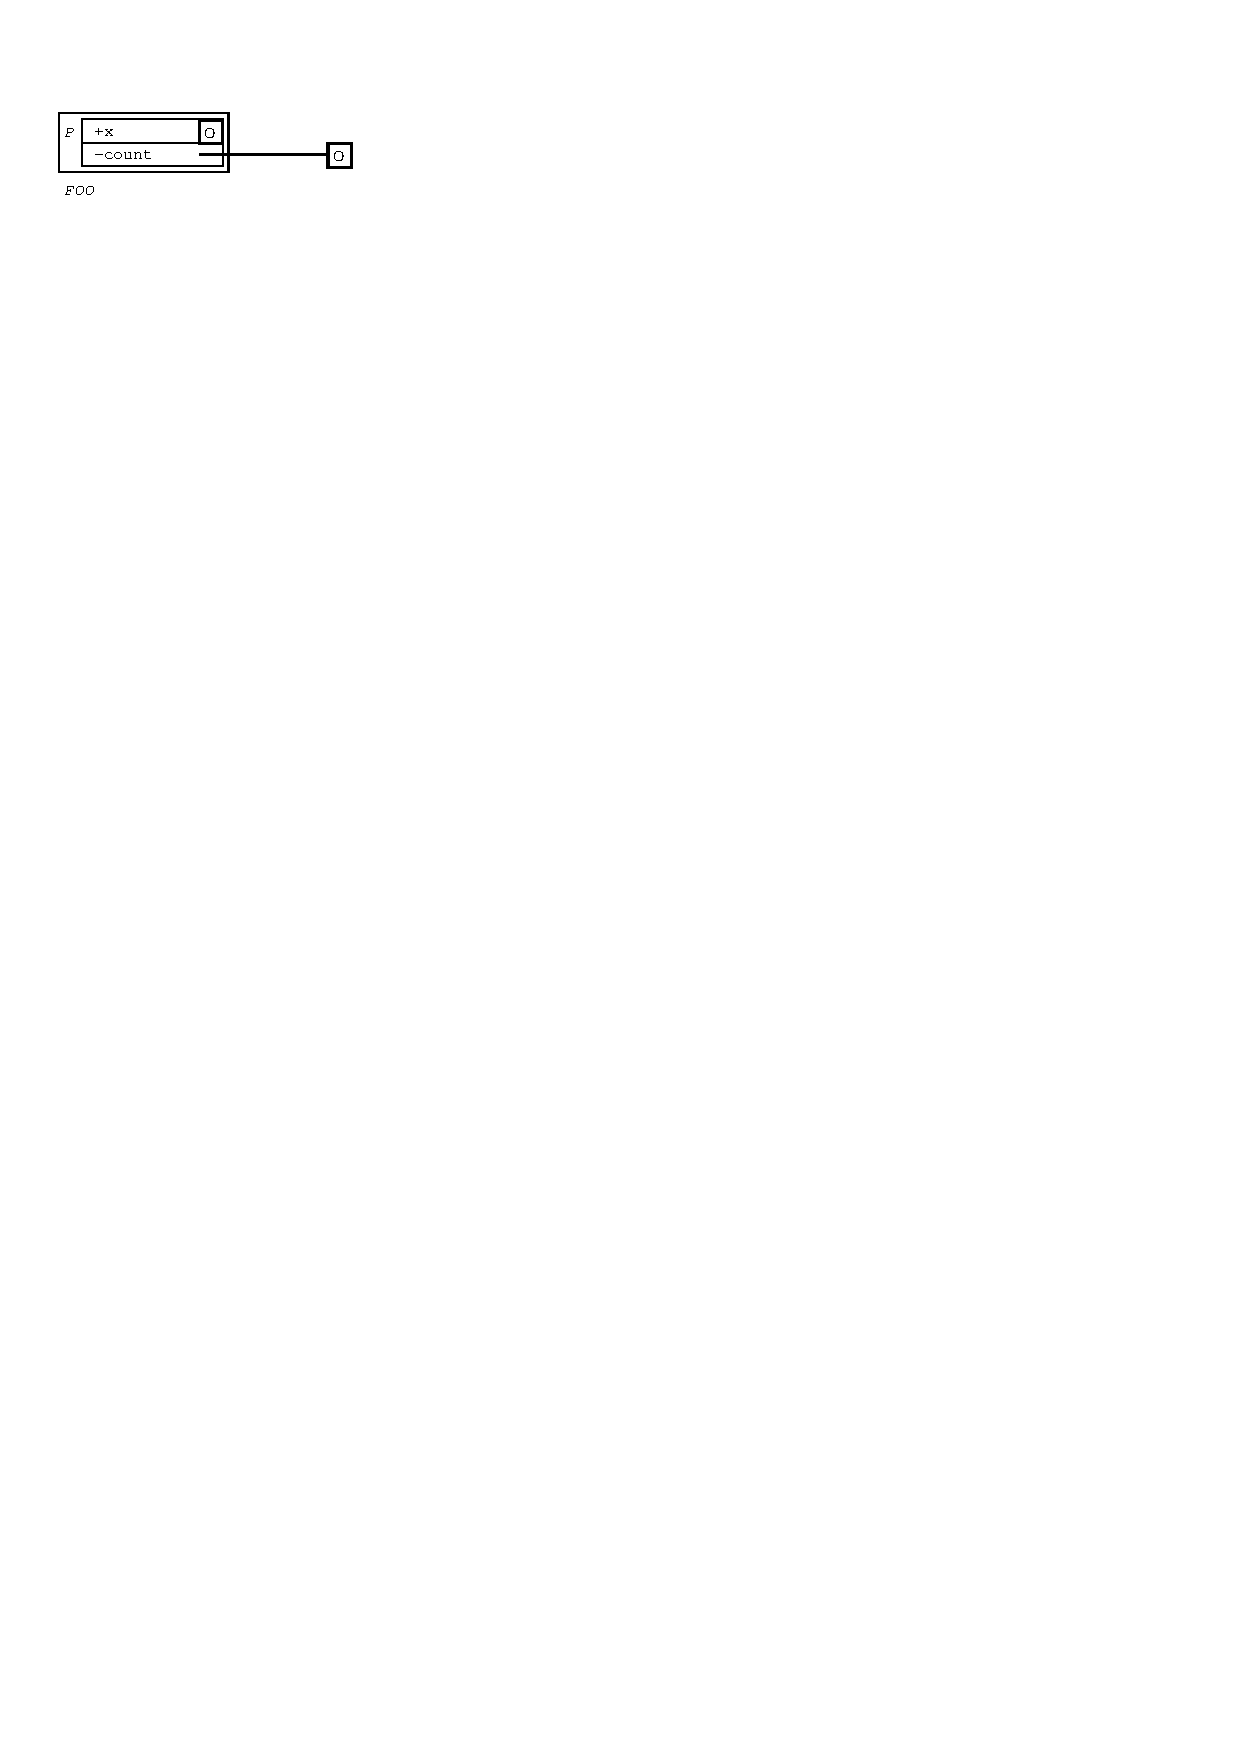
\includegraphics[scale=1.0]{figures/quick_clone0}
\end{center}

\begin{alltt}
  new\_foo := {\sc{}foo}.{\bf{}clone};
\end{alltt}

\begin{center}
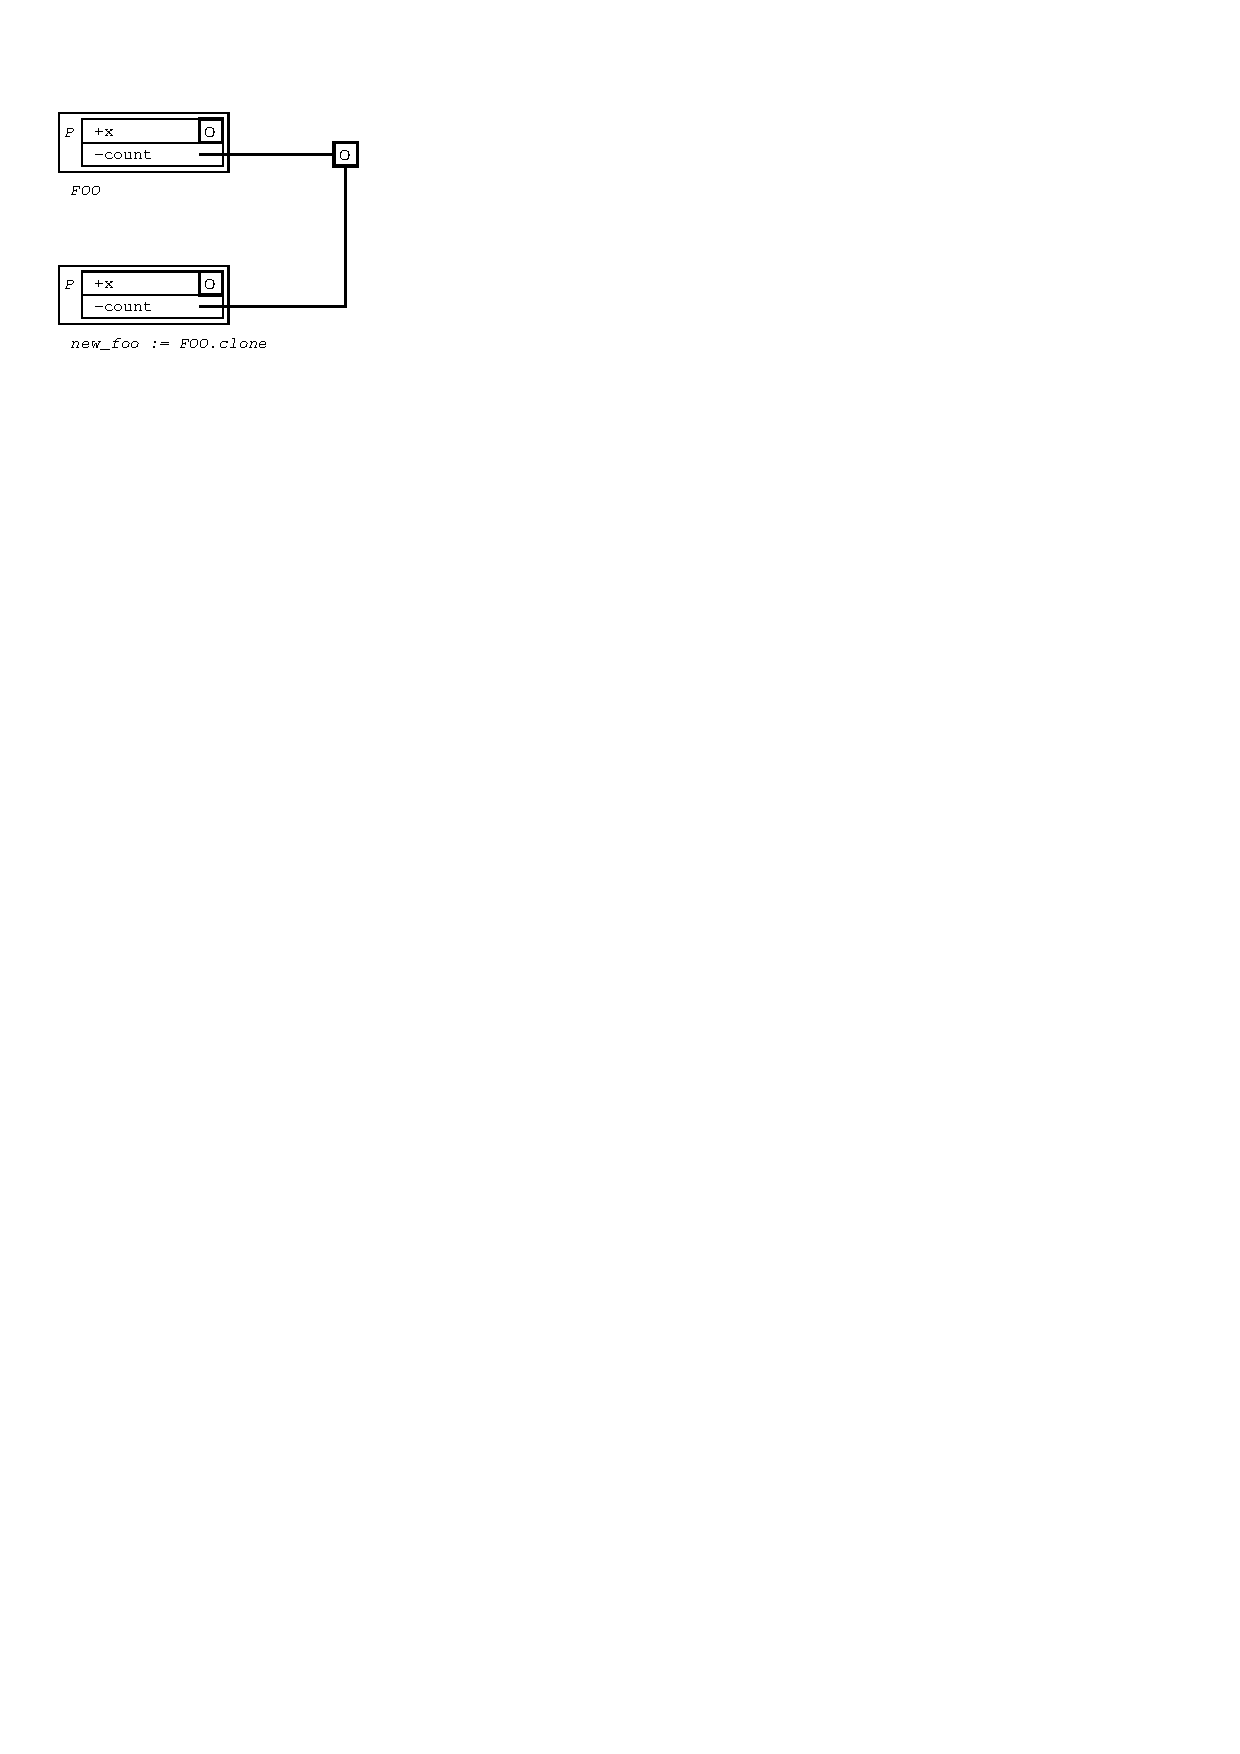
\includegraphics[scale=1.0]{figures/quick_clone1} 
\end{center}

\begin{alltt}
  new\_foo.{\bf{}set\_x} 1;
  new\_foo.{\bf{}set\_count} 2;
\end{alltt}

\begin{center}
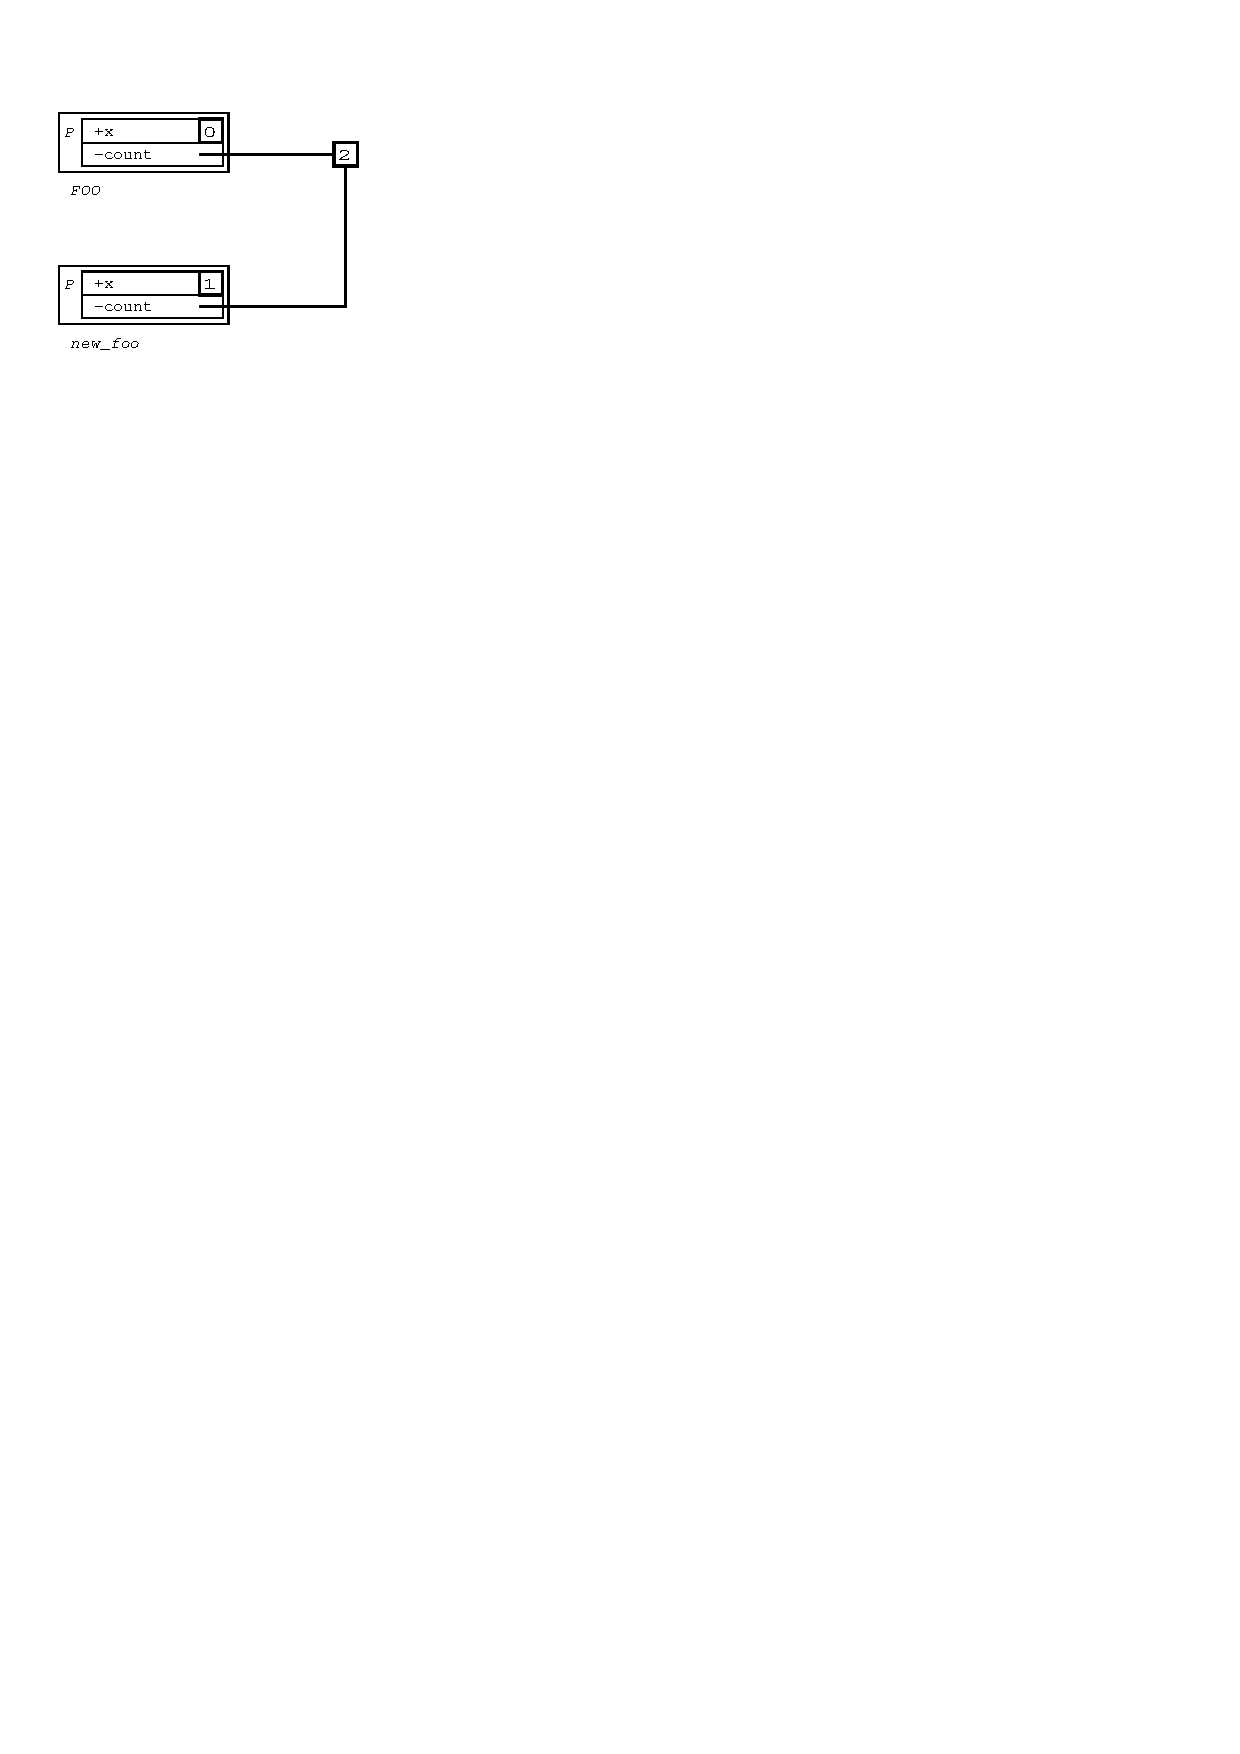
\includegraphics[scale=1.0]{figures/quick_clone2}
\end{center}

%---------------------------------------------------------
\subsection{Inheritance}
\label{quickstart:oo_language:inheritance}
%---------------------------------------------------------
%
\index{Inheritance}
You can define inheritance for objects. You can define as many parents as you want.
A parent is defined in a {\bf{}Section Inherit} with slots following the same rules as other slots.
A parent is also an object on which you can send messages.
If a slot called on an object is not found in this object, the {\it{}lookup} algorithm search in the parents to find the correct slot.
This algorithm do an ordered search from the first declared slot in the inheritance section.

{\it{}Example}: Let us see an inheritance with the parent defined with '-'
\index{Inheritance, shared}
\begin{center}
Object {\sc{}father}
\end{center}
\begin{alltt} 
{\bf{}Section Header}
  + {\bf{}name}     := {\sc{}father};          

{\bf{}Section Public}
  + {\bf{}x}    :{\sc{}integer};
  - {\bf{}inc\_x} <- ( x := x + 1; );
  - {\bf{}count}:{\sc{}integer};
  - {\bf{}inc\_count} <- ( count := count + 1; );
\end{alltt}
\begin{center}
Object {\sc{}son}
\end{center}
\begin{alltt} 
{\bf{}Section Header}
  + {\bf{}name}     := {\sc{}son};          

{\bf{}Section Inherit}
  - {\bf{}parent}:{\sc{}father} := {\sc{}father};       // name of the slot doesn't matter
{\bf{}Section Public}
  - {\bf{}change\_parent} p:{\sc{}father} <- ( parent := p; );
\end{alltt}
\begin{center}
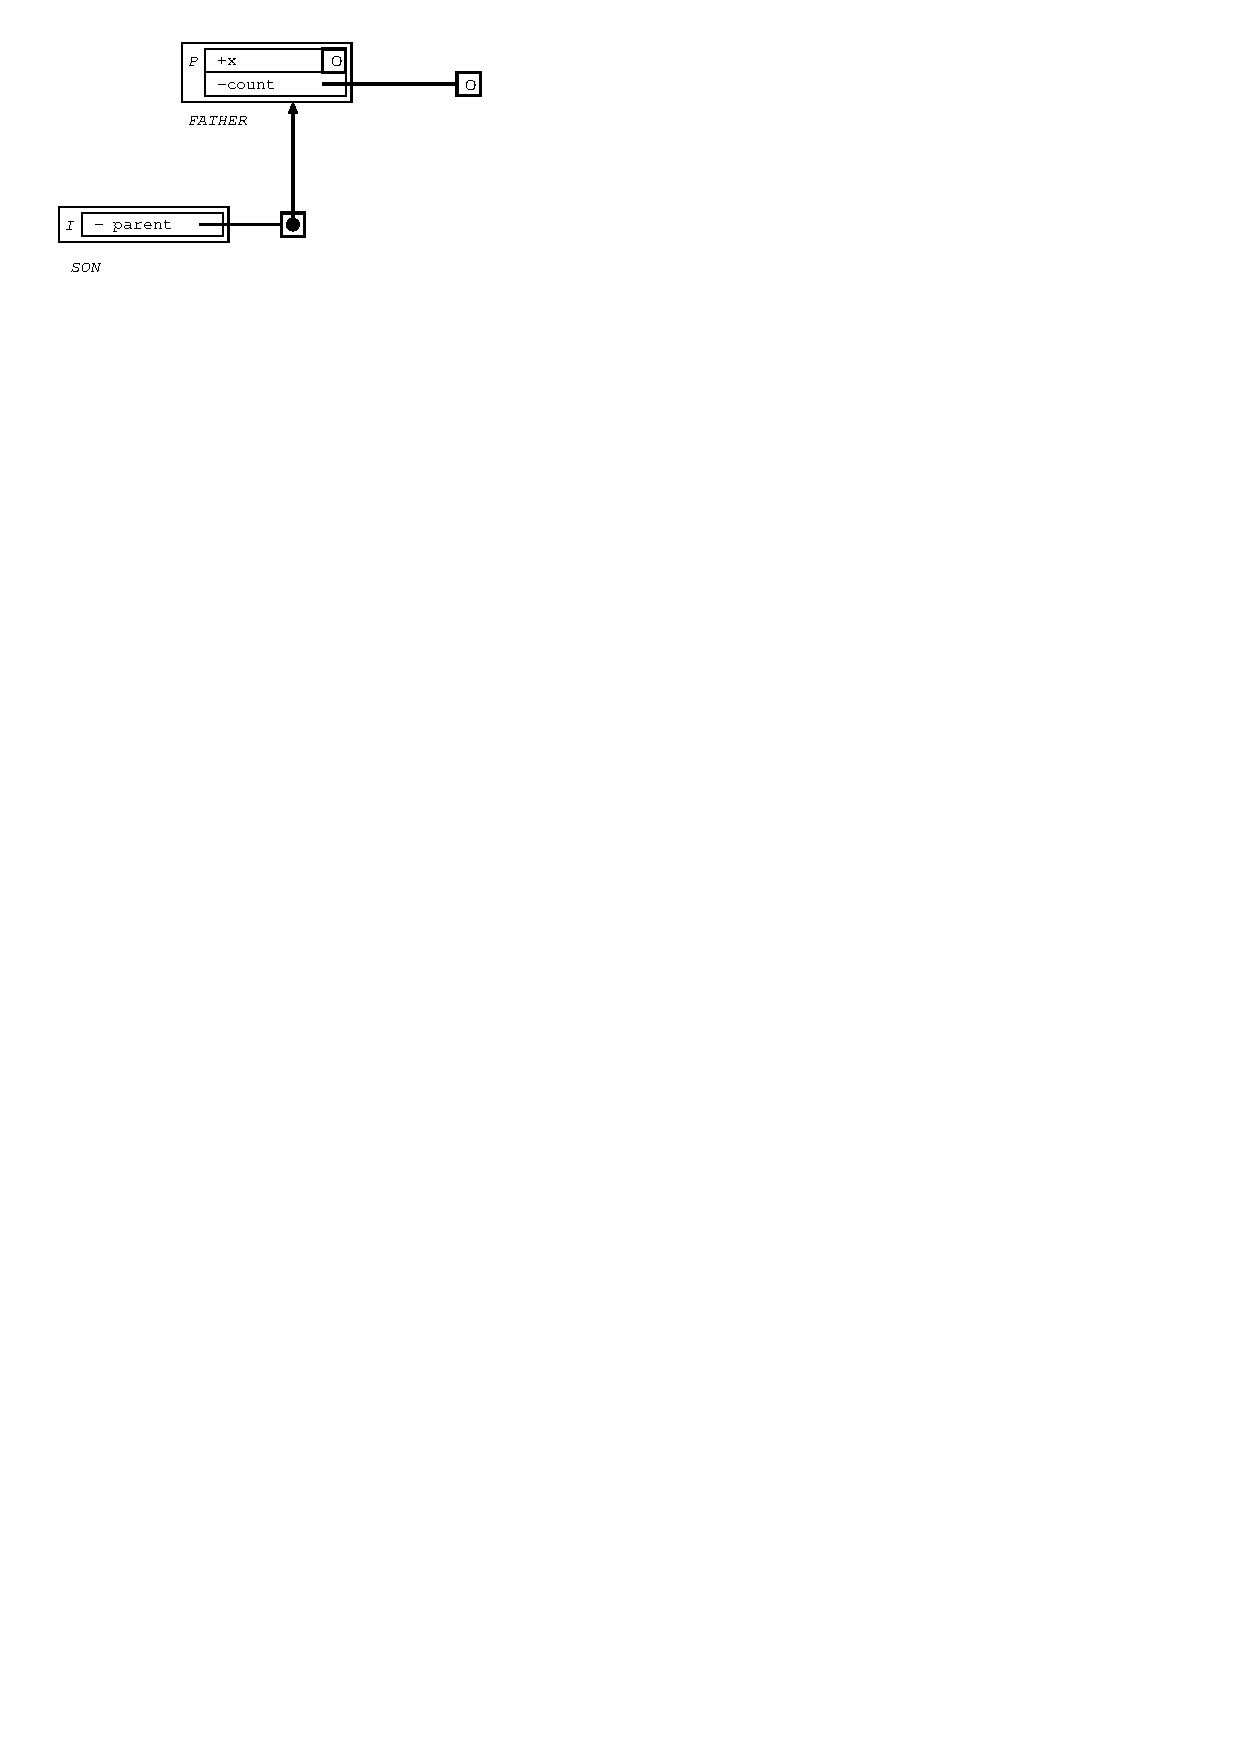
\includegraphics[scale=1.0]{figures/inherit_minus_0}
\end{center}

\begin{alltt}
  new\_son := {\sc{}son}.{\bf{}clone};
\end{alltt}
\begin{center}
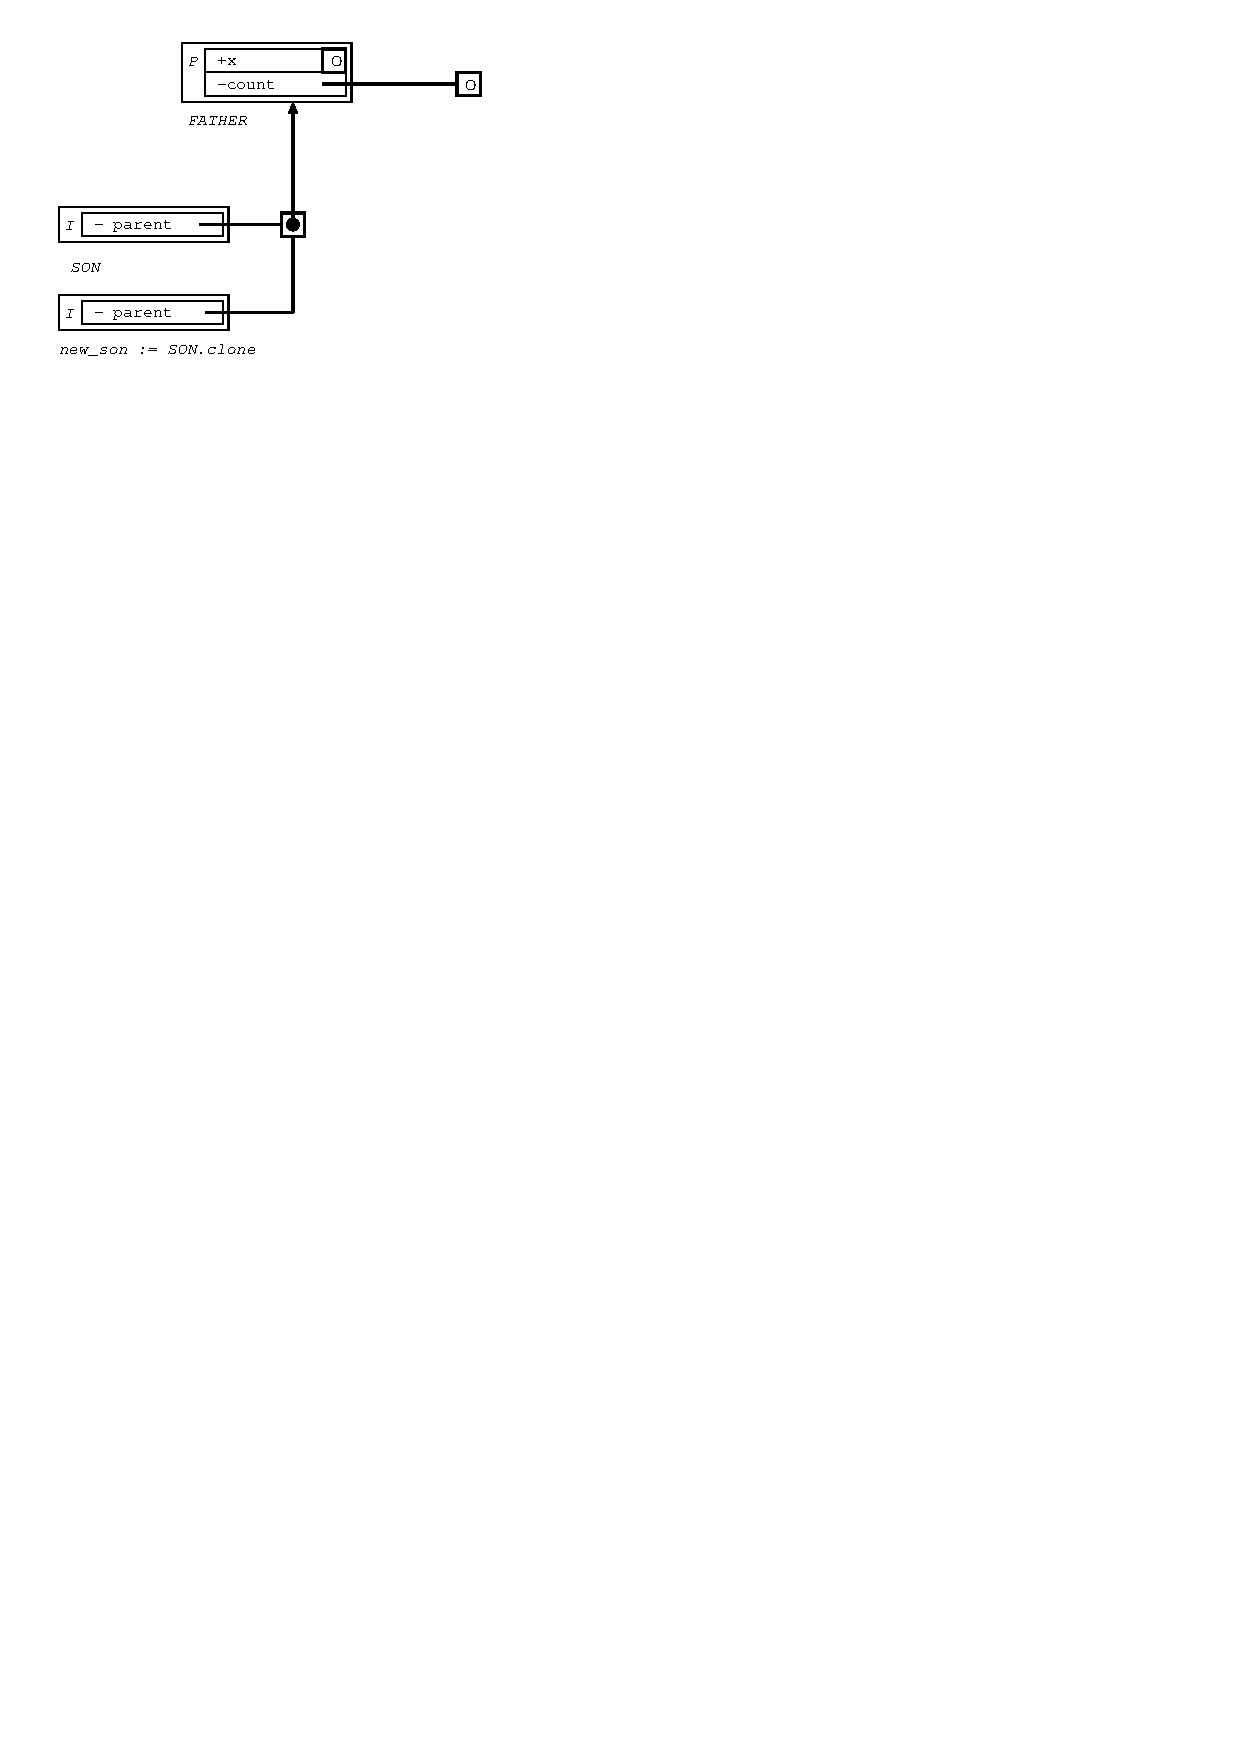
\includegraphics[scale=1.0]{figures/inherit_minus_1} 
\end{center}

\begin{alltt}
  new\_son.{\bf{}inc\_x};
  new\_son.{\bf{}inc\_count};
\end{alltt}
\begin{center}
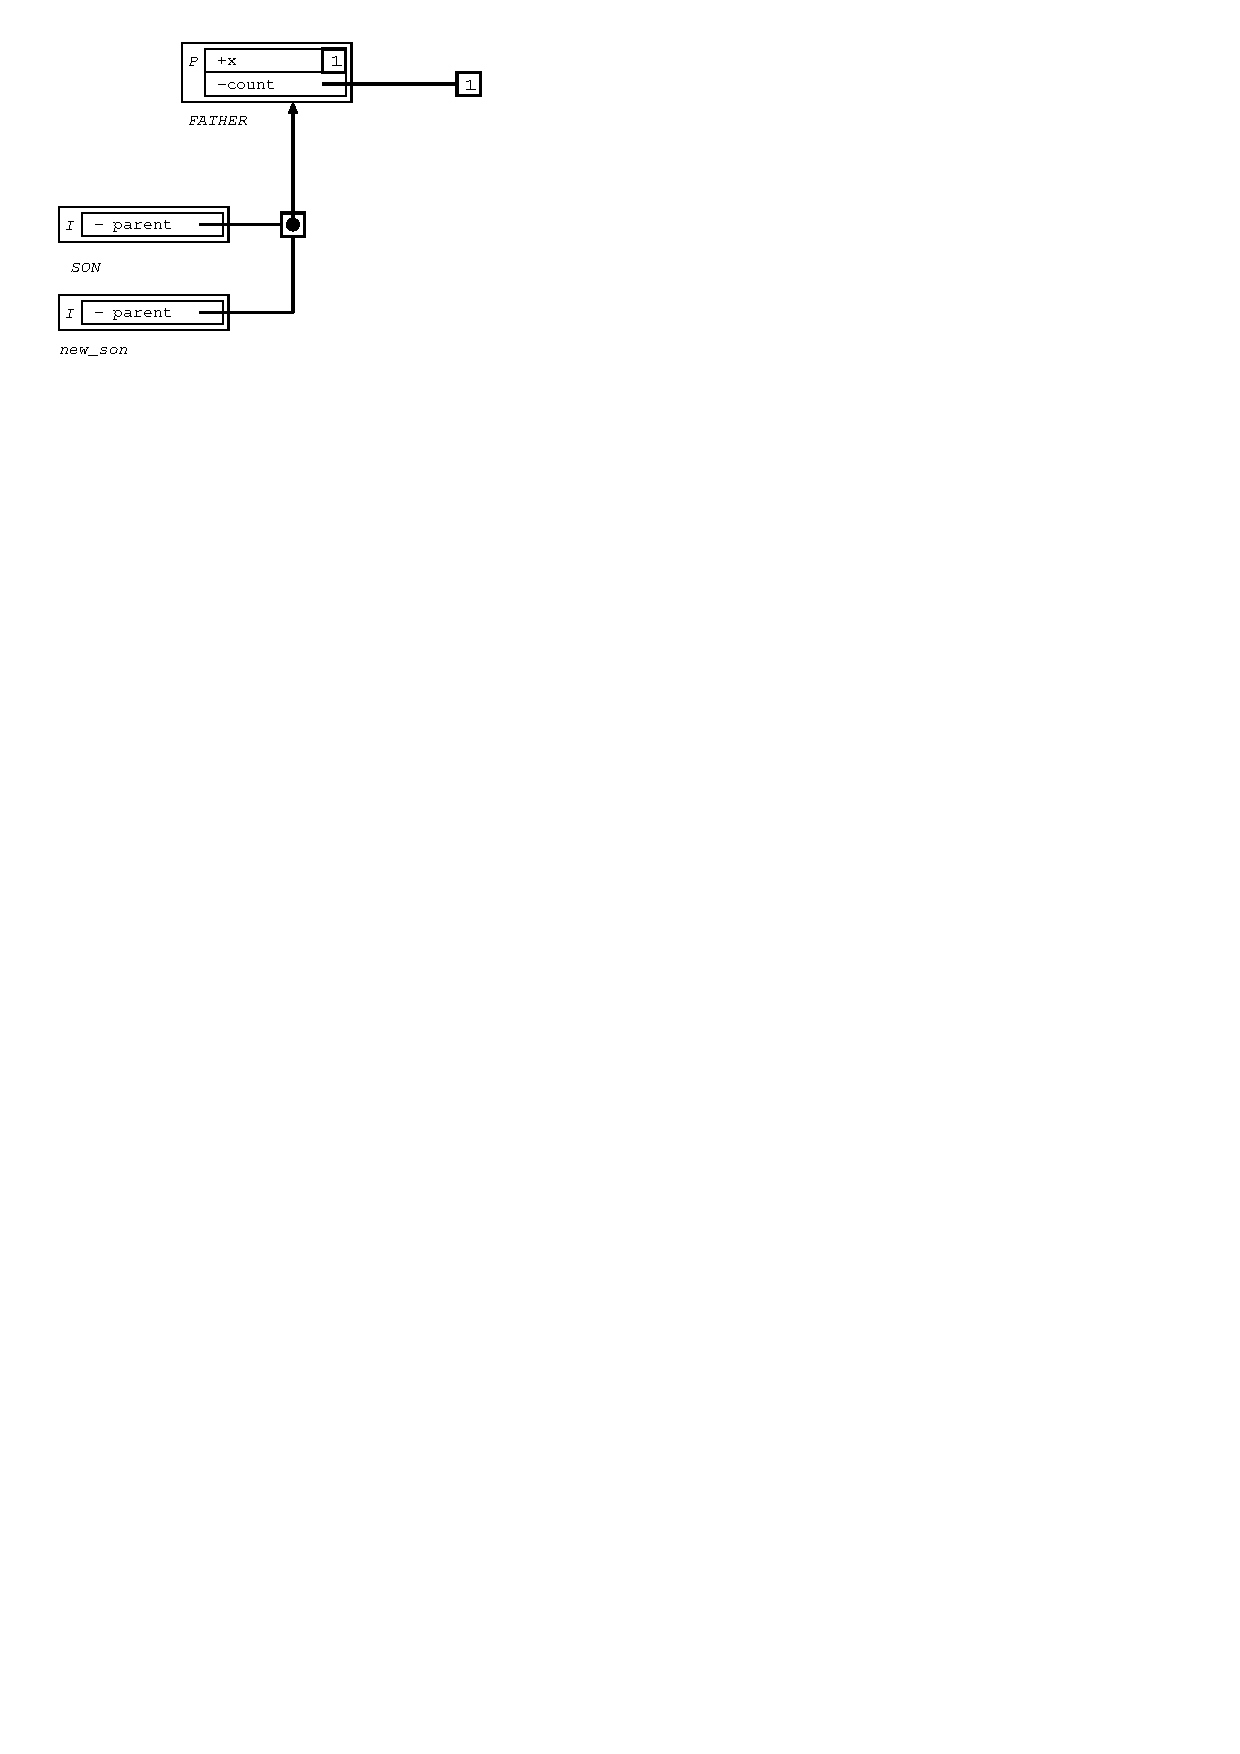
\includegraphics[scale=1.0]{figures/inherit_minus_2} 
\end{center}

\begin{alltt}
  new\_son.{\bf{}change\_parent} ({\sc{}father}.{\bf{}clone});
\end{alltt}
\begin{center}
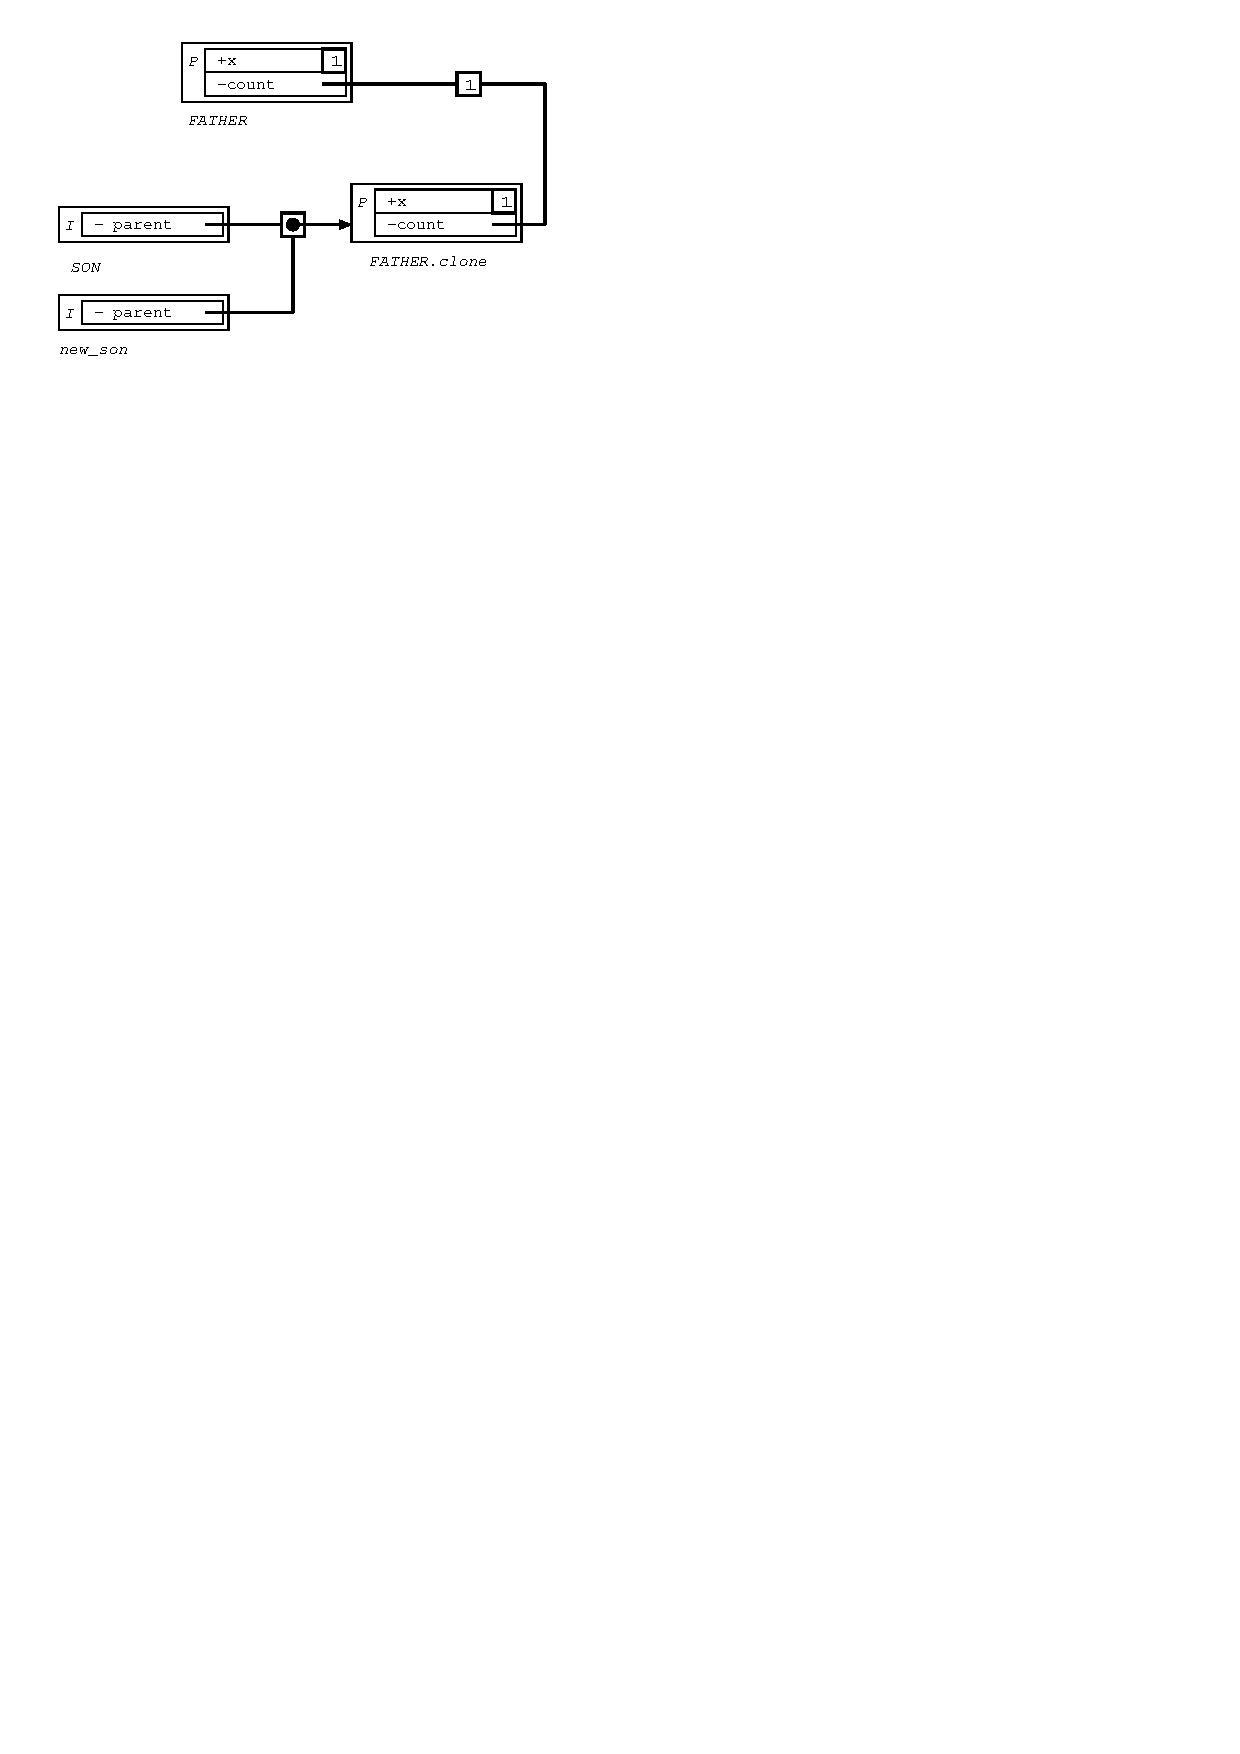
\includegraphics[scale=1.0]{figures/inherit_minus_3} 
\end{center}

\begin{alltt}
  new\_son.{\bf{}inc\_x};
  new\_son.{\bf{}inc\_count};
\end{alltt}
\begin{center}
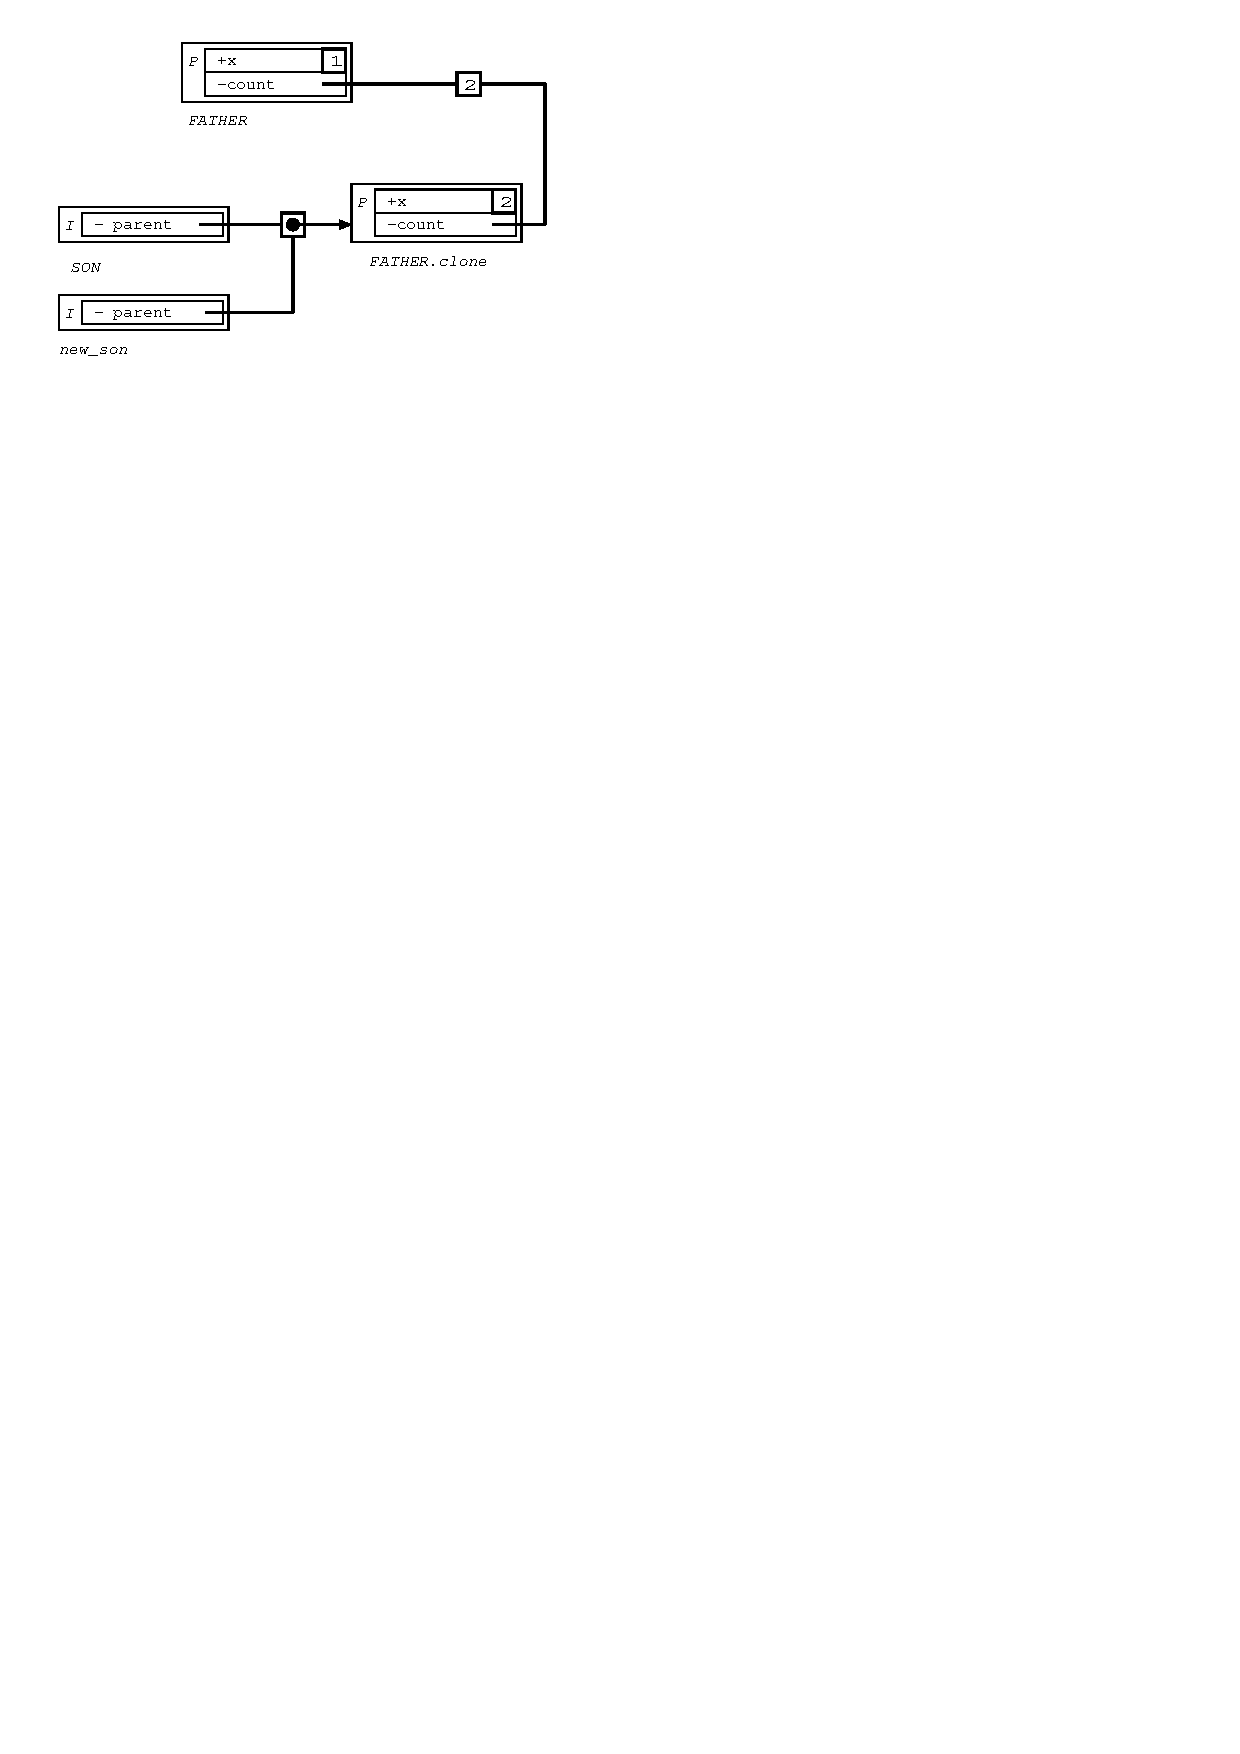
\includegraphics[scale=1.0]{figures/inherit_minus_4} 
\end{center}

{\it{}Example 2}: Let us see the same example with the parent defined with '+'
\index{Inheritance, non shared}
\begin{center}
Object {\sc{}father}
\end{center}
\begin{alltt}
{\bf{}Section Header}
  + {\bf{}name}     := {\sc{}father};          

{\bf{}Section Public}
  + {\bf{}x}    :{\sc{}integer};
  - {\bf{}inc\_x} <- ( x := x + 1; );
  - {\bf{}count}:{\sc{}integer};
  - {\bf{}inc\_count} <- ( count := count + 1; );
\end{alltt}
\begin{center}
Object {\sc{}son}
\end{center}
\begin{alltt} 
{\bf{}Section Header}
  + {\bf{}name}     := {\sc{}son};          

{\bf{}Section Inherit}
  + {\bf{}parent}:{\sc{}father} := {\sc{}father};
{\bf{}Section Public}
  - {\bf{}change\_parent} p:{\sc{}father} <- ( parent := p; );
\end{alltt}
\begin{center}
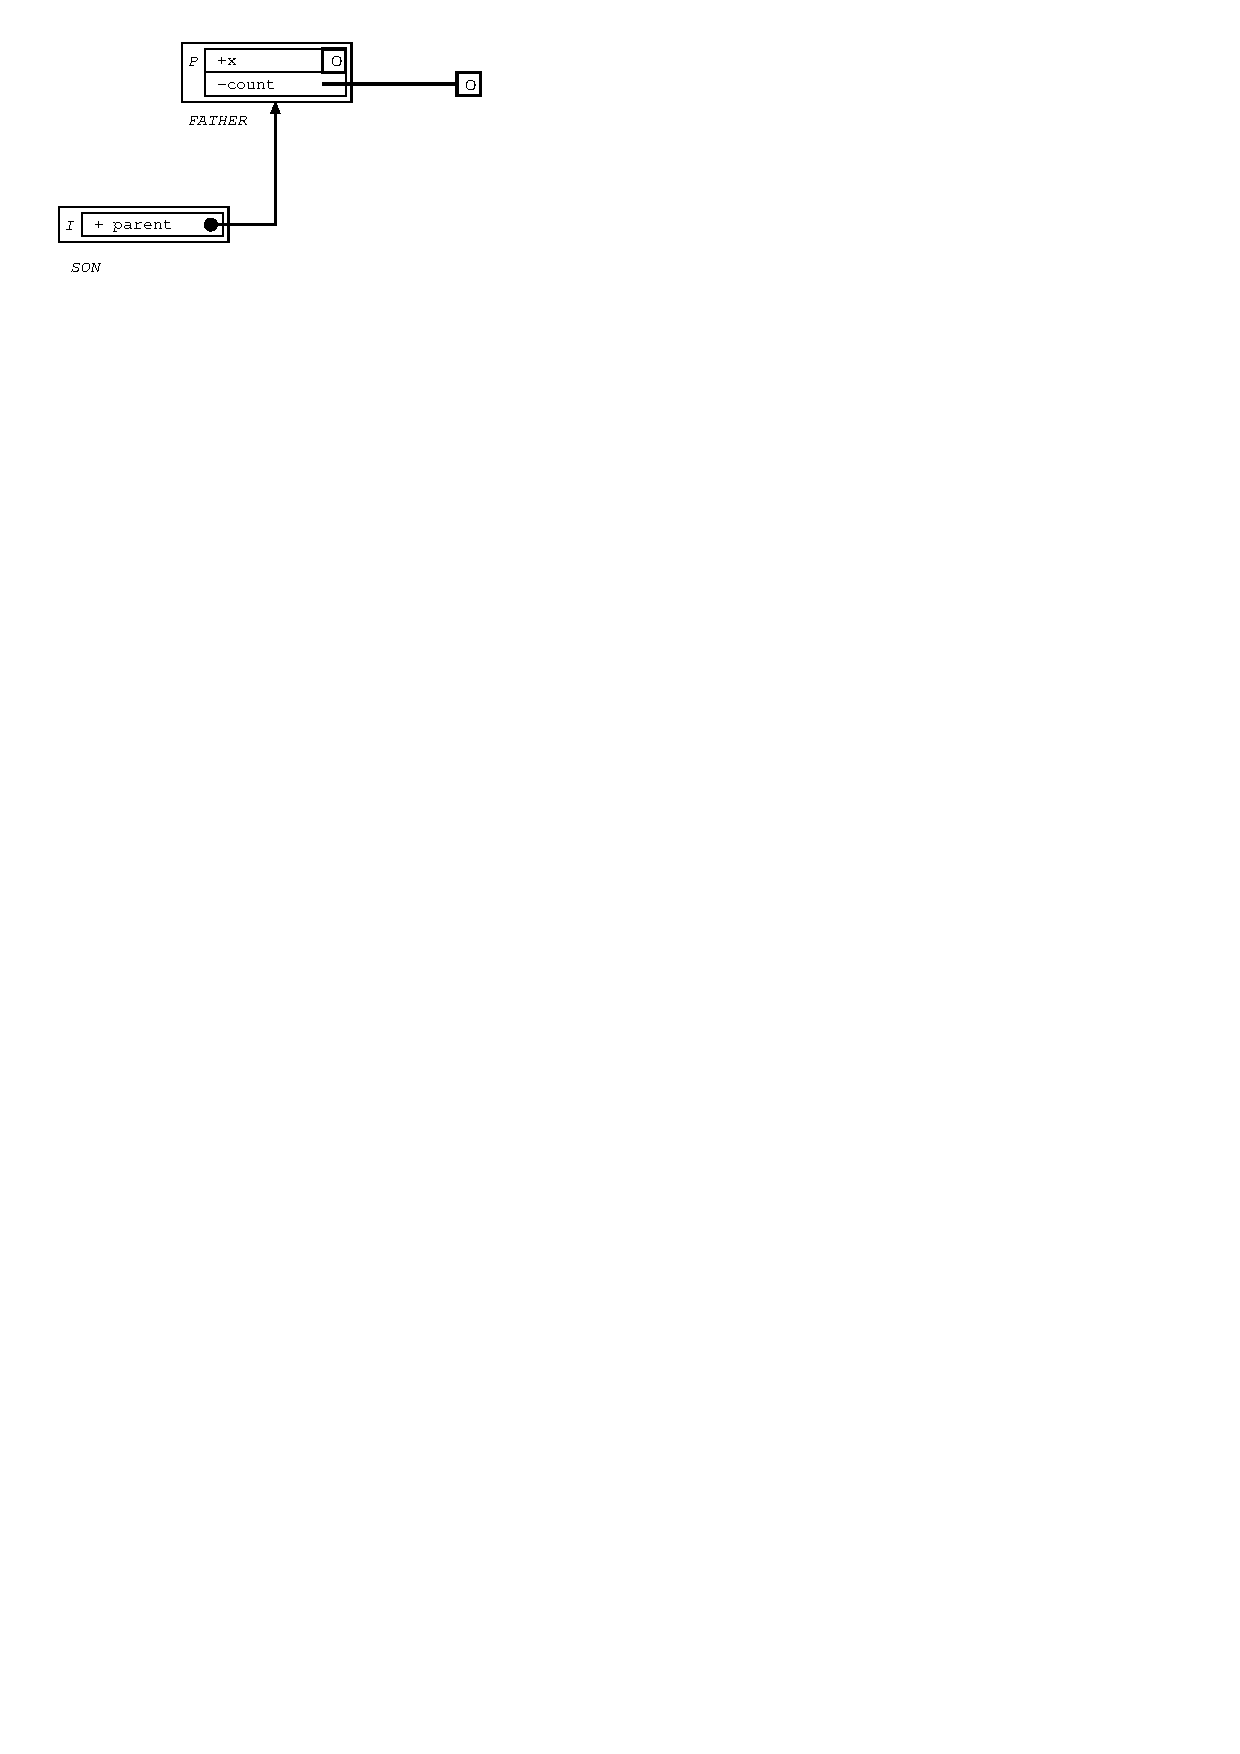
\includegraphics[scale=1.0]{figures/inherit_plus_0}
\end{center}

\begin{alltt}
  new\_son := {\sc{}son}.{\bf{}clone};
\end{alltt}
\begin{center}
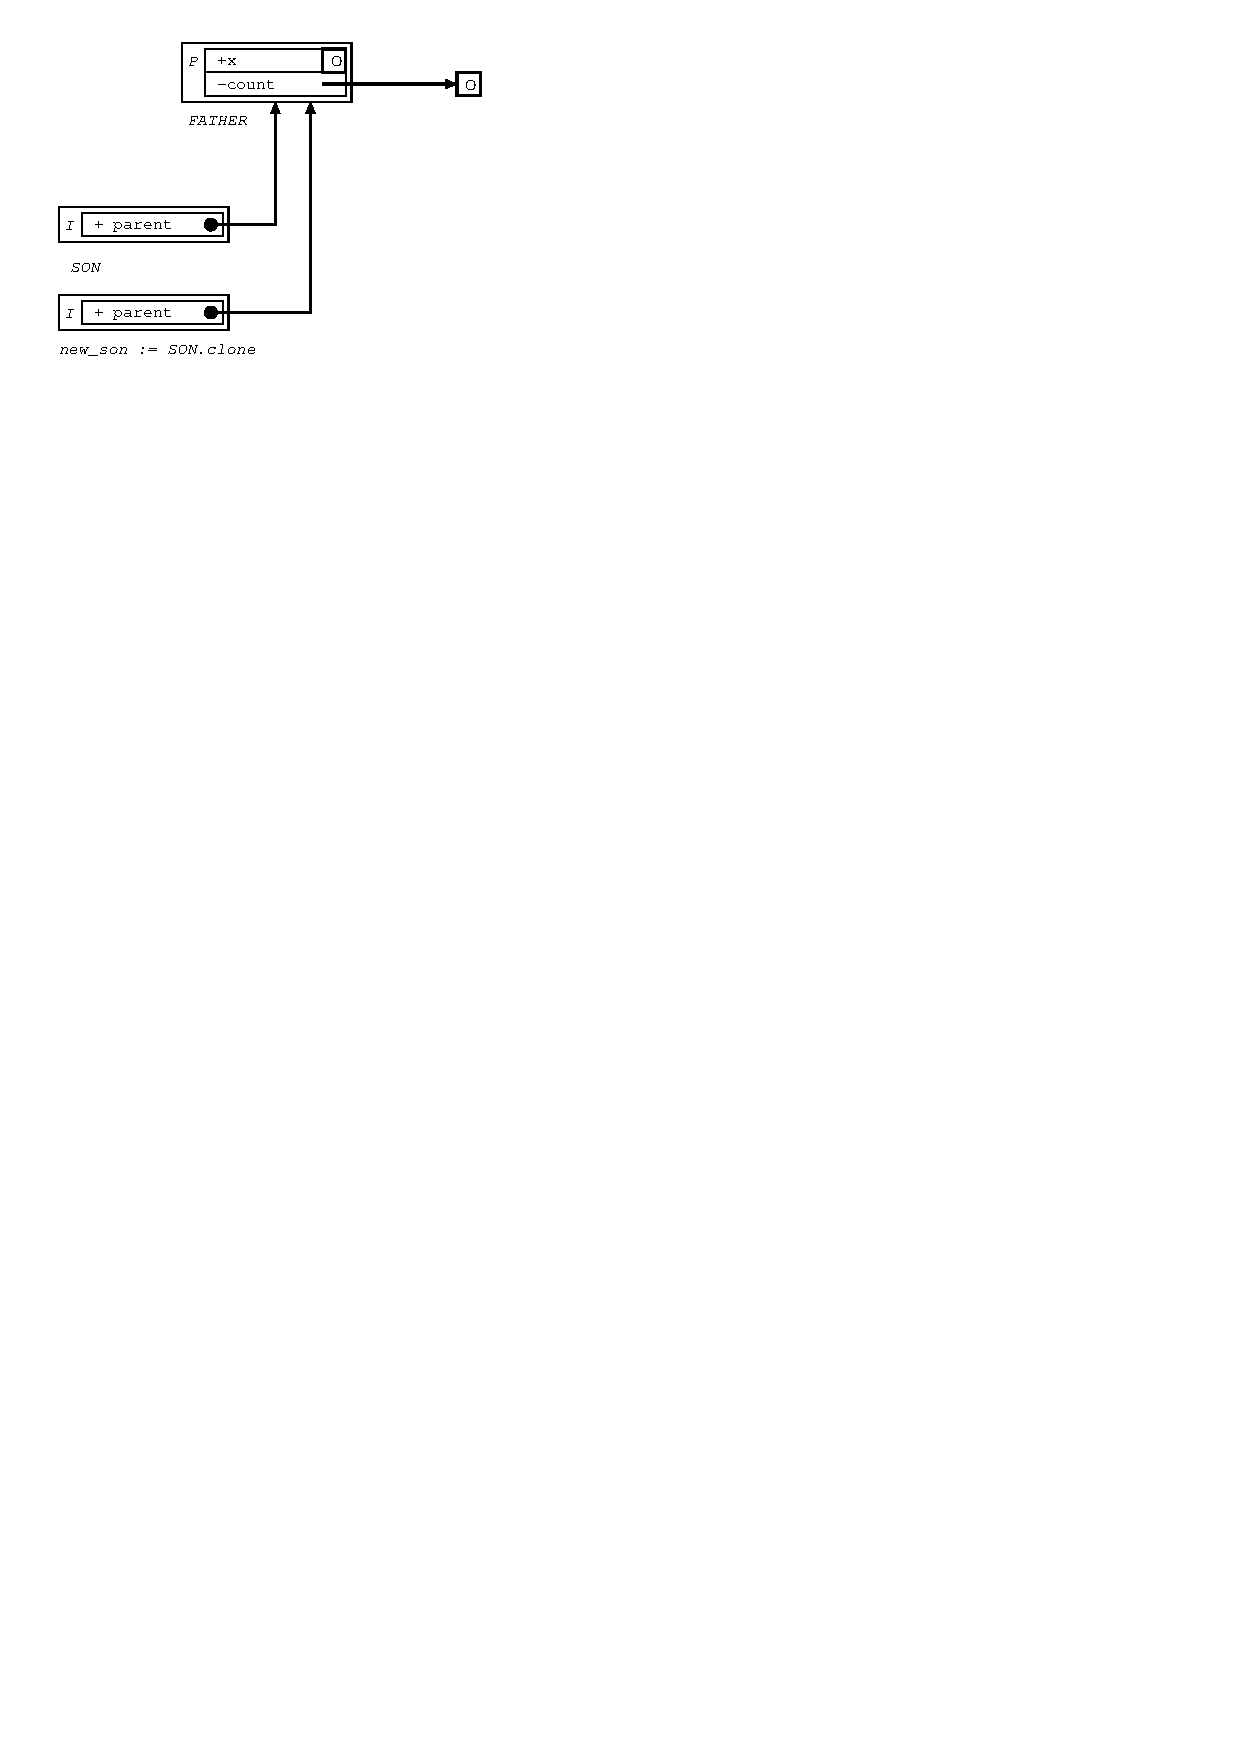
\includegraphics[scale=1.0]{figures/inherit_plus_1} 
\end{center}

\begin{alltt}
  new\_son.{\bf{}inc\_x};
  new\_son.{\bf{}inc\_count};
\end{alltt}
\begin{center}
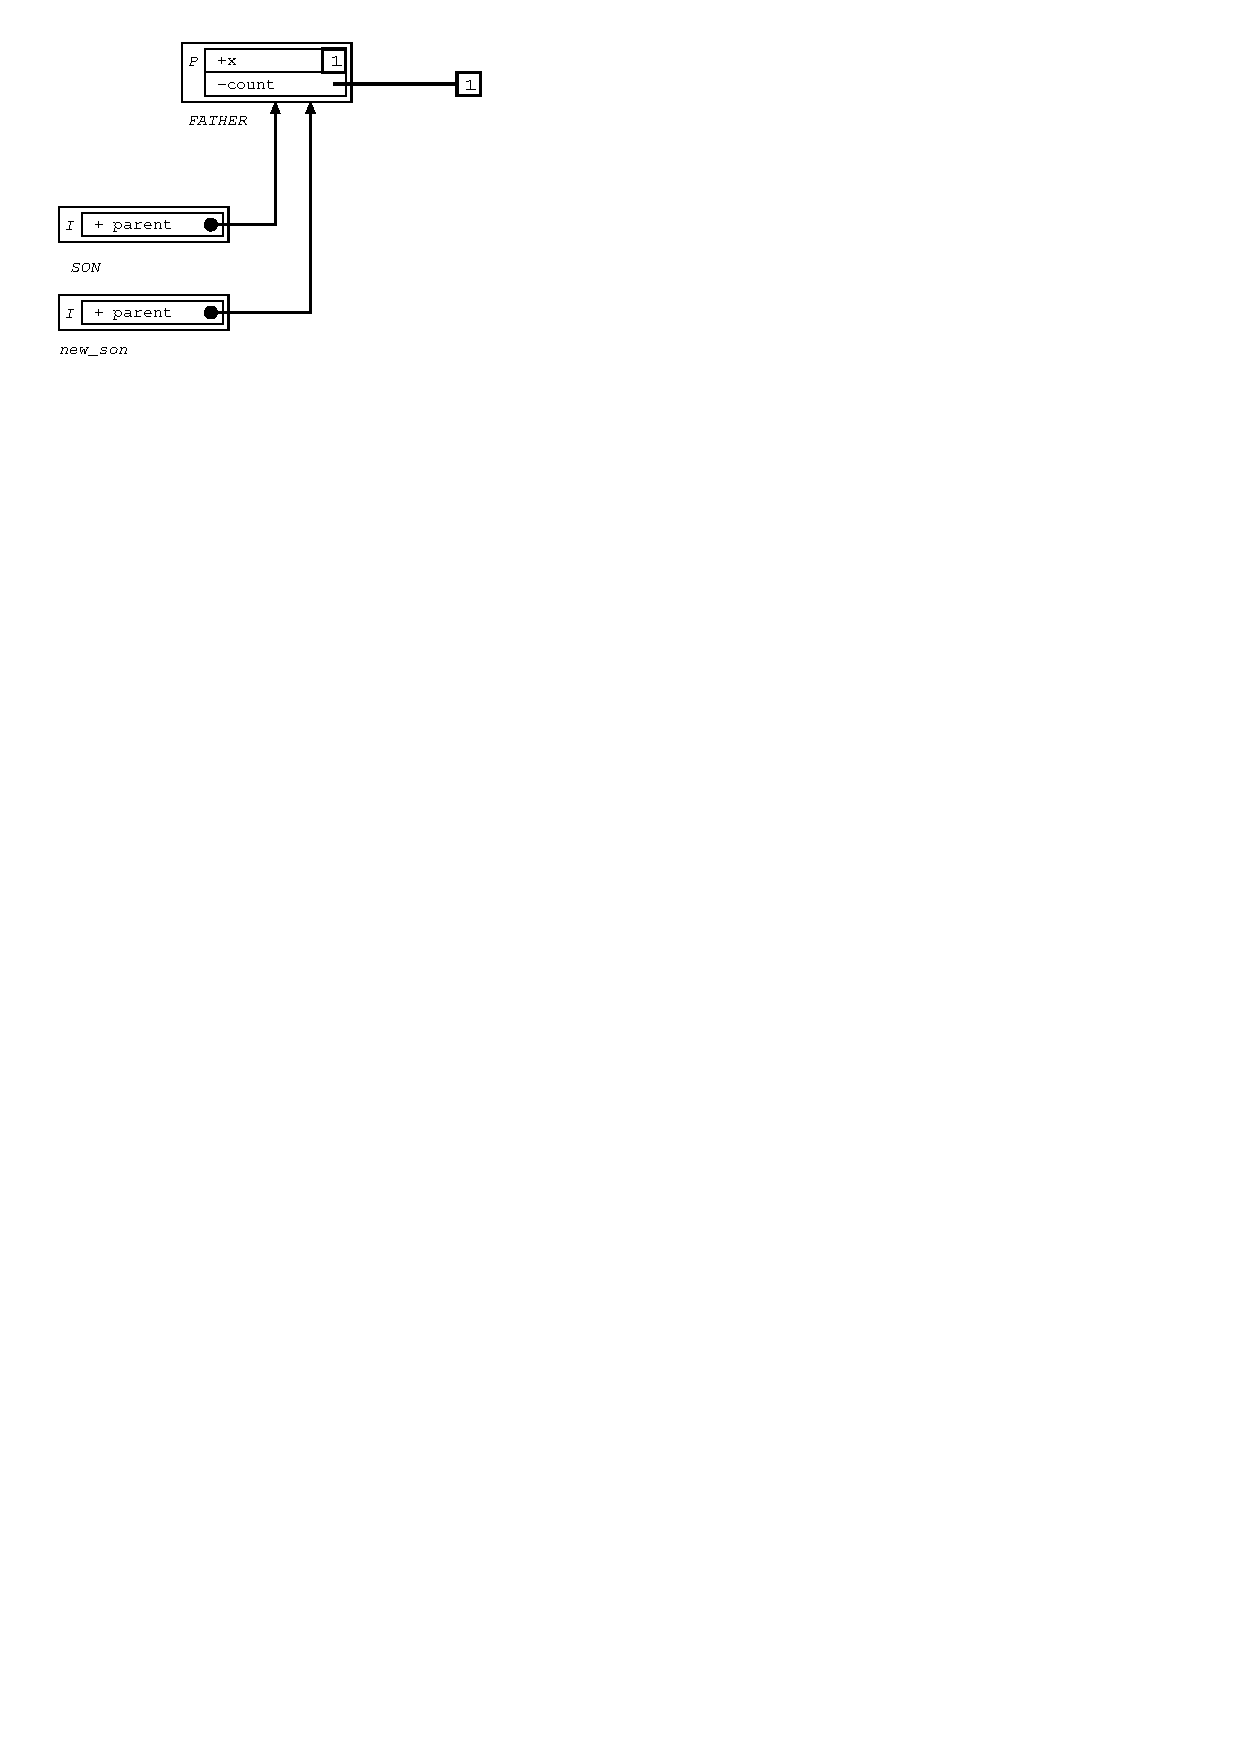
\includegraphics[scale=1.0]{figures/inherit_plus_2} 
\end{center}

\begin{alltt}
  new\_son.{\bf{}change\_parent} ({\sc{}father}.{\bf{}clone});
\end{alltt}
\begin{center}
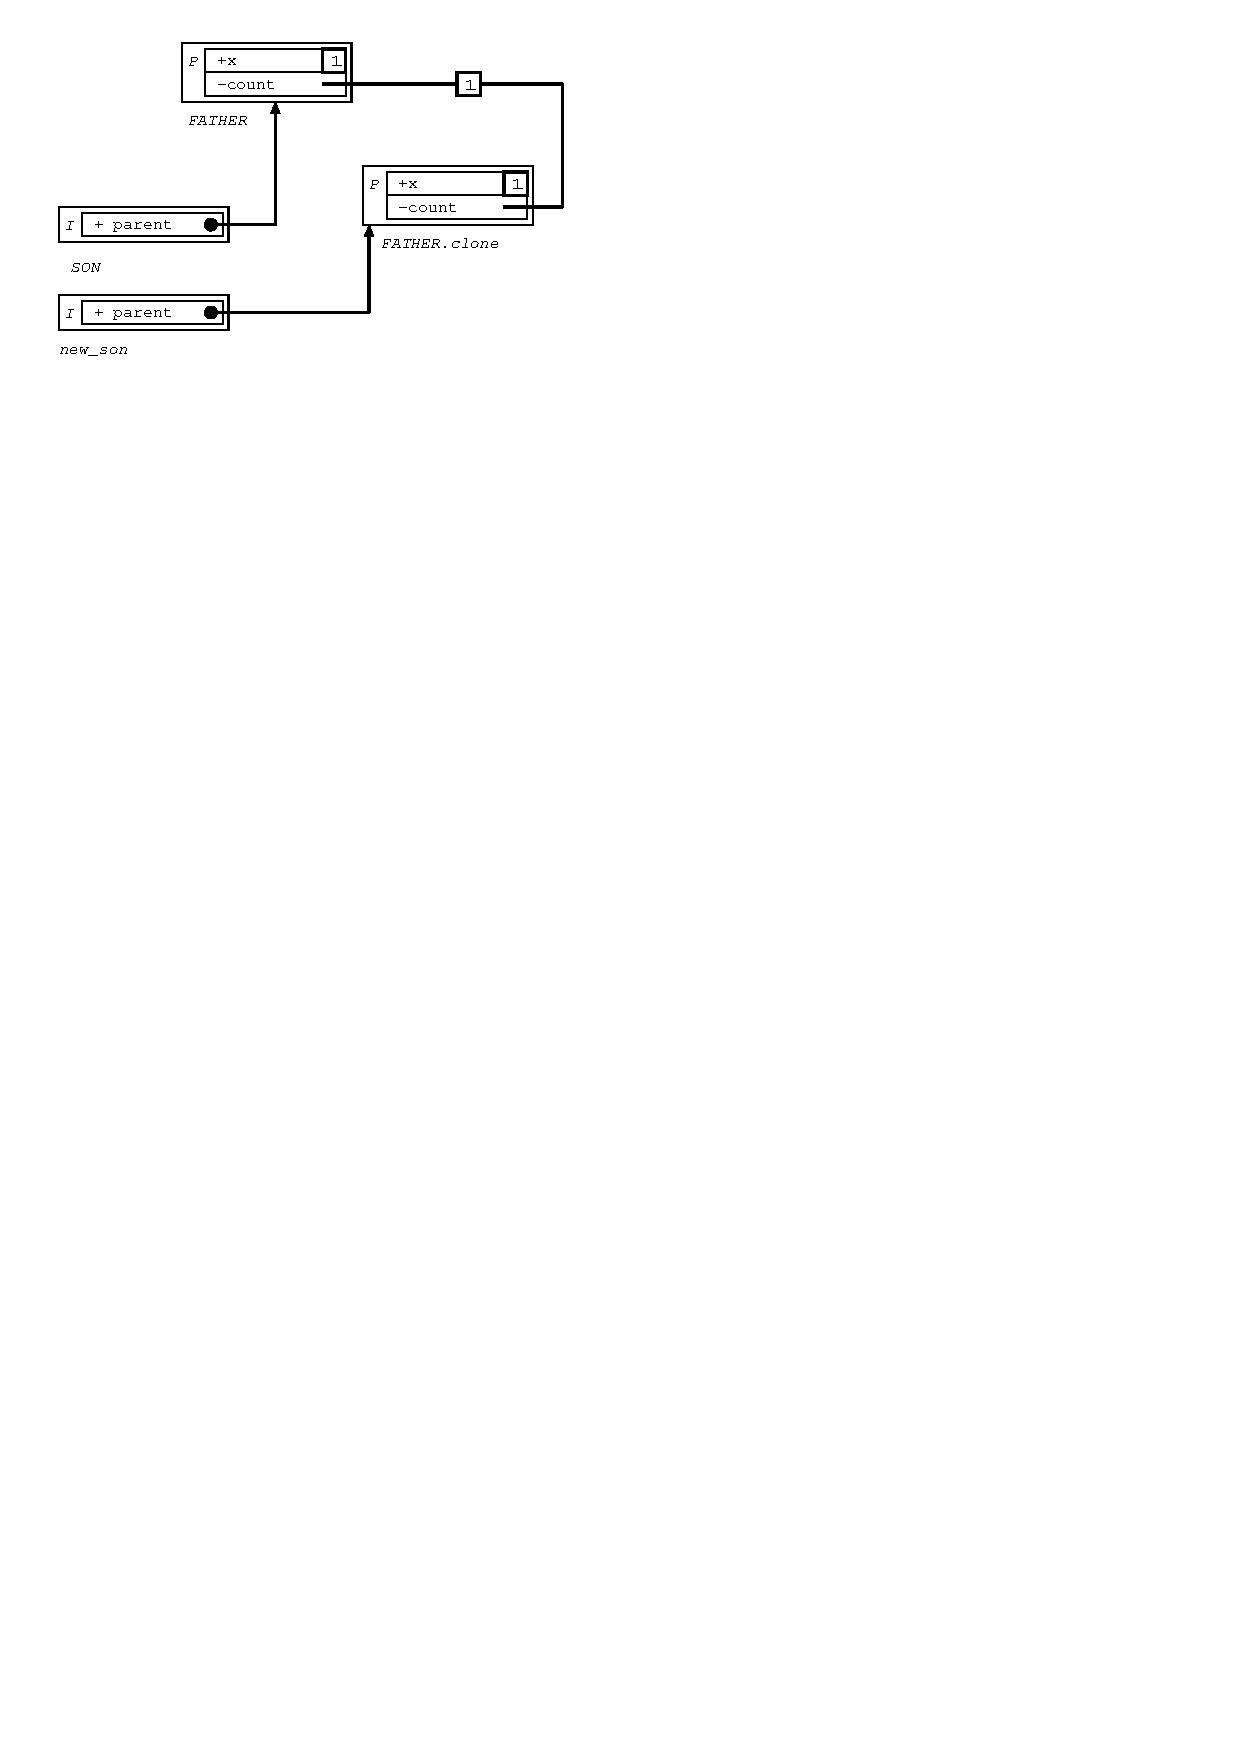
\includegraphics[scale=1.0]{figures/inherit_plus_3} 
\end{center}

\begin{alltt}
  new\_son.{\bf{}inc\_x};
  new\_son.{\bf{}inc\_count};
\end{alltt}
\begin{center}
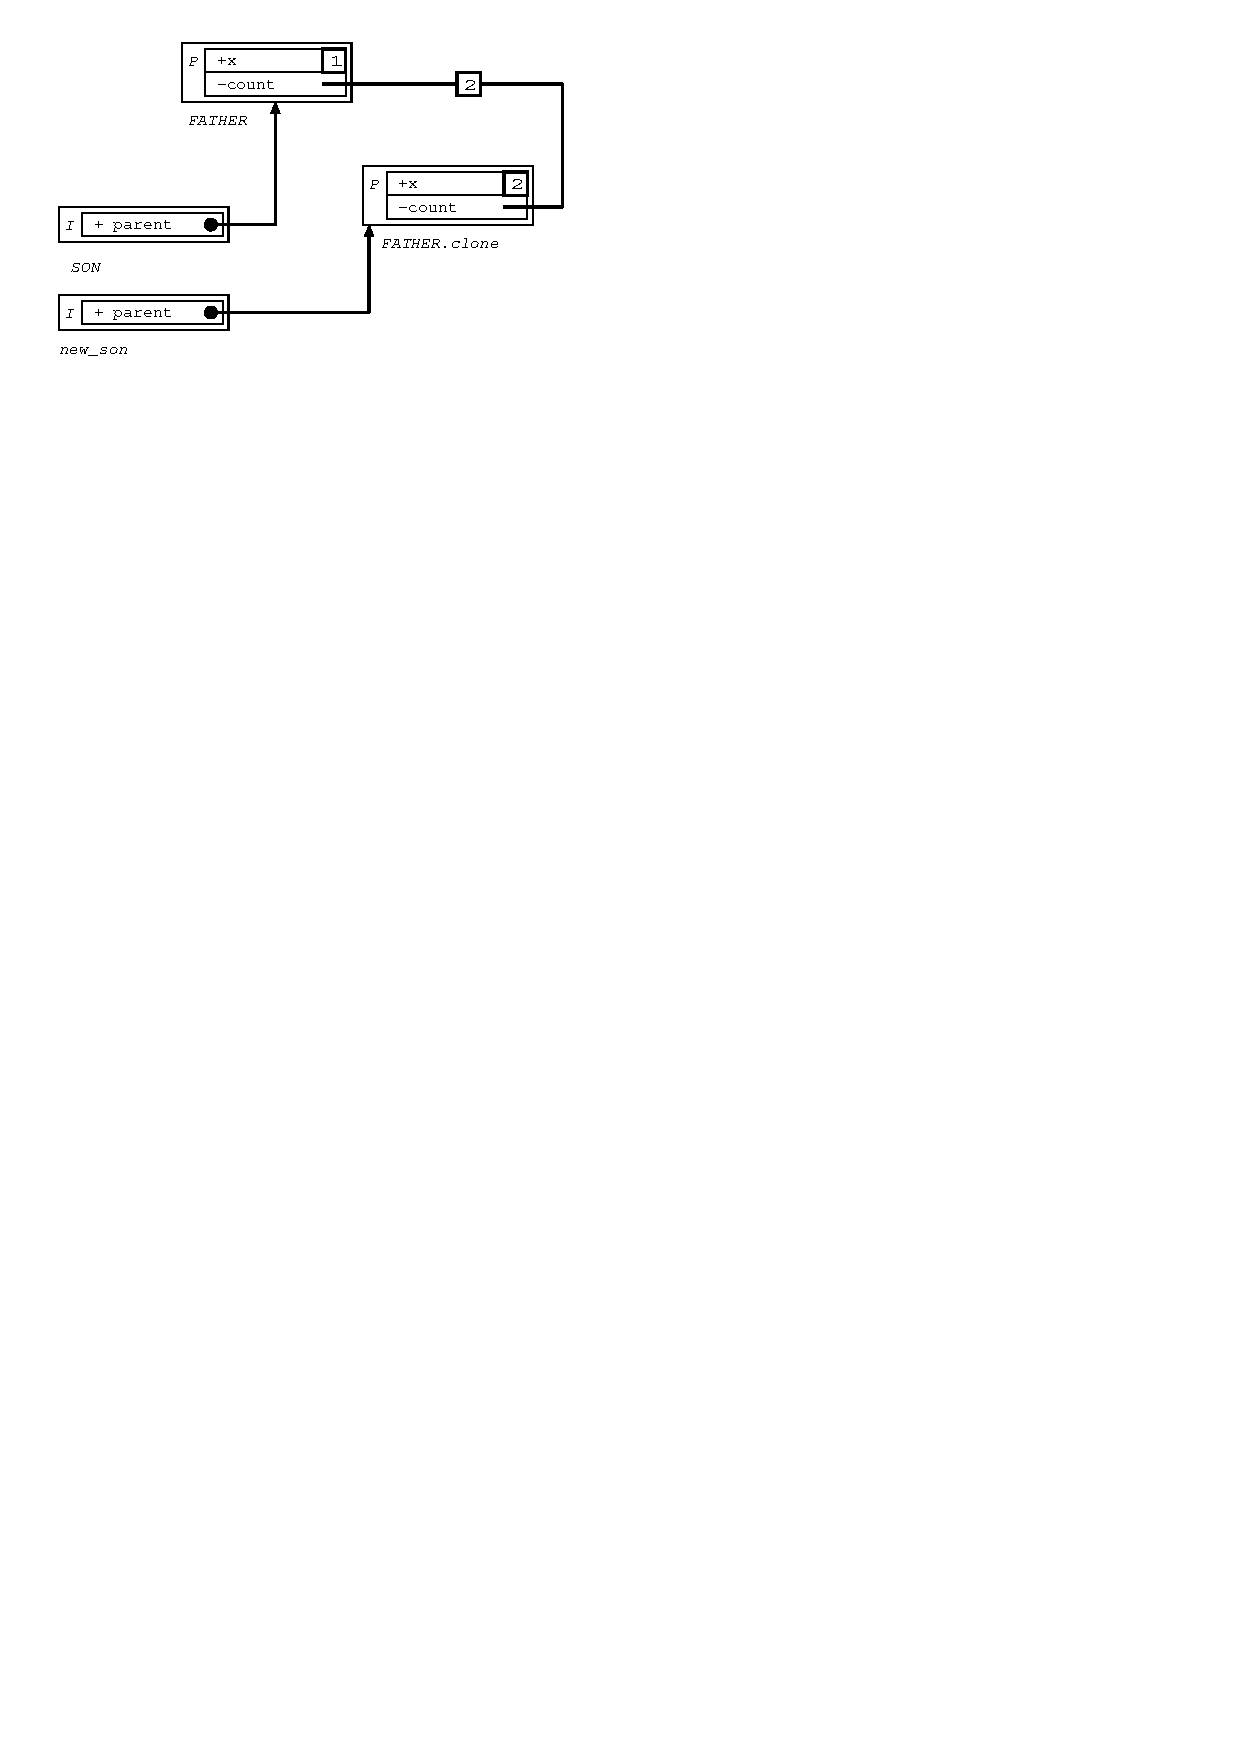
\includegraphics[scale=1.0]{figures/inherit_plus_4} 
\end{center}

%*********************************************************
\chapter{Language Reference}
\label{language_reference}
%*********************************************************

%=========================================================
\section{Lip: Lisaac project file (Lisaac Makefile)}
\label{language_reference:lip}
%=========================================================

Before entering deeper with the Lisaac language, the first step is to explain
how to compile a Lisaac program using Lip files. They are used to describe
compiler options, paths, include external libs even do inheritance between
projects.

\subsection{Lip Grammar}

The Lip grammar is a subset of the Lisaac grammar.

\begin{lstlisting}[frame=trBL]
PROGRAM      -> { 'Section' ('Inherit' | 'Public' | 'Private') { SLOT ';' } } 
SLOT         -> '+' identifier ':' TYPE [ ':=' EXPR_CONSTANT ]
              | '-' identifier [ identifier ':' TYPE ] '<-' EXPR  
TYPE         -> 'BOOLEAN' | 'STRING' | 'INTEGER' | 'LIP'
EXPR_AFFECT  -> [ identifier !!AMBIGU!! ':=' ] EXPR
EXPR         -> EXPR_CMP { ('|' | '&') EXPR_CMP }                
EXPR_CMP     -> EXPR_BINARY { ('='|'!='|'>'|'<'|'>='|'<=') EXPR_BINARY }
EXPR_BINARY  -> EXPR_UNARY { ('-'|'+') EXPR_UNARY }
EXPR_UNARY   -> ( '-' | '!' ) EXPR_UNARY
              | EXPR_BASE  
EXPR_LIST    -> { EXPR_AFFECT ';' } [ EXPR_AFFECT ]
EXPR_BASE    -> EXPR_RECEIVER { '.' EXPR_MESSAGE } 
EXPR_RECEIVER-> EXPR_PRIMARY 
              | EXPR_MESSAGE
EXPR_MESSAGE -> identifier [ EXPR_ARGUMENT ]              
              | 'if' '{' EXPR_LIST '}' [ 'else' '{' EXPR_LIST '}' ]              
EXPR_ARGUMENT-> identifier 
              | EXPR_PRIMARY
EXPR_PRIMARY -> EXPR_CONSTANT
              | '(' EXPR_LIST ')'
EXPR_CONSTANT-> integer              
              | string
              | TRUE
              | FALSE
\end{lstlisting}

\subsection{Example}

\begin{lstlisting}

Section Inherit

  + parent:STRING;

Section Private

  + is_valid:BOOLEAN;

  - src_path <-
  (
    path (lisaac + "src/*");
  );

  - front_end <-
  (
    general_front_end;
    ((input_file = "") | (input_file = "lisaac")).if {
      compiler_path;
      (is_valid).if {
        boost;
      };
    };
  );

  - back_end <-
  (
    general_back_end;
    (is_valid).if {
      execute "cp lisaac.c ../bin/.";
      execute "cp lisaac ../bin/.";
    };
  );

Section Public

  - compiler <-
  // Compile the Lisaac compiler.
  (
    compiler_path;
  );
\end{lstlisting}


\subsection{Lip usage and features}

The compiler always needs a Lip file to work. By default the compiler will look
in the default Lip file found in the Lisaac environnement variable path
\textbf{LISAAC\_DIRECTORY} or with the old way in the path.h. This will appear
if tou don't have a Lip file for your project, otherwise the compiler will at
first read the Lip file in the directory you are calling the compiler. The
compiler look in the current directory and in all parents to find a
\textit{make.lip} file. If no inheritance is set, the \textit{make.lip} file
from the compiler is inherited. You can also add inheritance by hand with this
two ways:

\begin{lstlisting}

  + parent : STRING;
  + parent := "../../../path../file";

\end{lstlisting}

The \textbf{+} is used for variables and \textbf{-} for methods.\\

In the \textit{Private Section}, variables and functions will not appear to the
compiler. You can then use this Section to describe things you want to be done
before the compiler is working and to set options you want to call in the
\textit{Public Section} with the compiler. All compiler options are thus
described in the \textit{Public Section}. \\

When you add a public function, It is possible to add a commentary down to the
function definition, then when calling the compiler this description and
arguments will appear as show this example:\\


\begin{lstlisting}
Section Public
  
  - debug level:INTEGER <-
  // Fix debug level (default: 15)
  (
    // some code
  );

================================================================

$lisaac

Usage:                                                          
  lisaac [<lip_file.lip>] [<input_file[.li]>] {<Options>}       
                                                                  
Options:          
  ...
  -debug <level:INTEGER> :
    Fix debug level (default: 15)
  ...
\end{lstlisting}


\subsection{Advanced Lip usage}

Some builtin methiods are part of the compiler:

\begin{itemize}
\item \textbf{exit}: exit from function as in C
\item \textbf{path(STRING)}: add prototype path location
\item \textbf{run(STRING)}: execute the string as a unix command
\item \textbf{get\_integer}: get command line integer
\item \textbf{get\_string}: get command line string\\
\end{itemize}

For describing a path you can use the \textbf{*} symbol as for example:
\textit{lisaac/personnal/*}.\\

\noindent{}Compiling steps:

\begin{enumerate}
\item The compiler look for a \textit{make.lip} file
\item the front\_end method is runned
\item compilation and C generation
\item the back\_end method is runned
\end{enumerate}


%=========================================================
\section{Lexical and syntax overview}
\label{language_reference:lexical_syntax}
%=========================================================
%
Most features of Lisaac come from the Self language.
Like Self, Lisaac does not have hard-coded instructions for loops
or test statements.

The following syntax of Lisaac is described using 
"Extended Backus-Naur Form" (EBNF).
Terminal symbols are enclosed between single quotes or are written using 
lowercase letters. 
Non-terminal are written using {\bf{}uppercase} letters.
\index{Semantic}
The following table describes the semantic of meta-symbols
used:

\noindent
\begin{tabularx}{\textwidth}{c l X}
\hline
{\bf{}Symbol}    & {\bf{}Function} & {\bf{}Description} \cr
\hline
\hline
{( /* \ldots */ )}     & {grouping}      & {a group of syntactic constructions} \cr
\hline
{[ /* \ldots */ ]}     & {option}        & {an optional construction} \cr
\hline
{\{ /* \ldots */ \}}   & {repetition}    & {a repetition (zero or more times)} \cr
\hline
{{\tt |}}        & {alternative}   & {separates alternative constructions} \cr
\hline
{$\rightarrow$}  & {production}    & {separates the left and right hand sides of a production} \cr
\hline
\end{tabularx}

\noindent

%---------------------------------------------------------
\subsection{Lexical overview}
\label{language_reference:lexical_syntax:lexical}
%---------------------------------------------------------
%
\index{Final elements, grammar}
The following rules draw up the list of the final syntactic 
elements of the grammar:\\
\noindent
\begin{tabularx}{\textwidth}{l X}
\hline
{\bf{}Symbol} & {\bf{}Description} \\                
\hline
\hline
{\it{}section}         & {section identifier} \\     
\hline
{\it{}identifier}      & {slot name, \ldots} \\     
\hline
{\it{}operator}        & {unary or binary operator symbol} \\
\hline
{\it{}integer}         & {constant of type {\sc{}integer}} \\
\hline
{\it{}real}            & {constant of type {\sc{}real}} \\
\hline
{\it{}cap\_identifier} & {type name: name of object or prototype} \\     
\hline
{\it{}characters}      & {constant of type {\sc{}character} } \\
\hline
{\it{}string}          & {constant of type {\sc{}string} } \\
\hline
{\it{}external}        & {external C code} \\
\hline
{\it{}affect}          & {symbol assignment slots} \\
\hline
{\it{}style}           & {clone comportement} \\
\hline
{\it{}type}            & {unary typing operation} \\
\hline
{\it{}result}          & {result identifier value} \\
\hline
\end{tabularx}

\noindent
{\tt\begin{tabular}{lrl}
{\it{}section} & $\rightarrow$ & "Header"\,|\,"Inherit"\,|\,"Private"\,|\,"Public"\\
               & |\,           & "Mapping"\,|\,"Interrupt"\,|\,"Directory"\\
               & |\,           & "External"\,|\,"Insert"\\

{\it{}identifier} & $\rightarrow$ & LOWER\_CASE\,\{\,LOWER\_CASE\,|\,DECIMAL\_DIGIT\,|\,'\_'\,\}\\

{\it{}operator}   & $\rightarrow$ & OP\_CHAR\,\{\,OP\_CHAR\,\} {\it{}except affect symbol and } '=' {\it{}or} '!='\\

{\it{}integer}    & $\rightarrow$ & OCTAL\_DIGIT\,\{\,OCTAL\_DIGIT\,|\,'\_'\,\}\,'o'\\
                  & |\,           & DECIMAL\_DIGIT\,\{\,DECIMAL\_DIGIT\,|\,'\_'\,\}\,[\,'d'\,]\\
                  & |\,           & HEXA\_DIGIT\,\{\,HEXA\_DIGIT\,|\,'\_'\,\}\,'h'\\

{\it{}real}       & $\rightarrow$ & DECIMAL\_DIGIT\,\{\,DECIMAL\_DIGIT\,|\,'\_'\,\}\,'.'\,[\,\{\,DECIMAL\_DIGIT\,\}\,]\\
{}                &               & [\,'E'\,['+'|'-']\,DECIMAL\_DIGIT\,\{\,DECIMAL\_DIGIT\,\}\,]\\

{\it{}cap\_identifier} & $\rightarrow$ & UPPER\_CASE\,\{\,UPPER\_CASE\,|\,DECIMAL\_DIGIT\,|\,'\_'\,\}\\

{\it{}characters}  & $\rightarrow$ & '''\,(\,NORMAL\_CHAR\,|\,ESCAPE\_CHAR\,)\,'''\\

{\it{}string}      & $\rightarrow$ & '"'\,\{\,NORMAL\_CHAR\,|\,ESCAPE\_CHAR\,\}\,'"'\\

{\it{}external}    & $\rightarrow$ & '`'\,\{\,NORMAL\_CHAR\,|\,ESCAPE\_CHAR\,\}\,'`'\\

{\it{}affect}      & $\rightarrow$ & ":="\,|\,"<-"\,|\,"?="\\

{\it{}style}       & $\rightarrow$ & '+'\,|\,'-'\\

{\it{}type}        & $\rightarrow$ & "Expanded"\,|\,"Separate"\,|\,"Strict"\\

{\it{}result}      & $\rightarrow$ & "Result"\,\{\,'\_' DECIMAL\_DIGIT\,\{\,DECIMAL\_DIGIT\,\}\,\}\\

OP\_CHAR      & $\rightarrow$ & {\tt '!'\,|\,'@'\,|\,'\#'\,|\,'\$'\,|\,'\%'\,|\,'$\wedge$'\,|\,'\&'\,|\,'$<$'\,|\,'|'} \\
              & |\,       & {\tt '*'\,|\,'+'\,|\,'-'\,|\,'='\,|\,'$\sim$'\,|\,'/'\,|\,'?'\,|\,'$>$'\,|\,'$\backslash$'}\\

LOWER\_CASE   & $\rightarrow$ & 'a'\,|\,'b'\,|\,\ldots\,|\,'z'\\

UPPER\_CASE   & $\rightarrow$ & 'A'\,|\,'B'\,|\,\ldots\,|\,'Z'\\

OCTAL\_DIGIT  & $\rightarrow$ & '0'\,|\,'1'\,|\,\ldots\,|\,'7'\\

DECIMAL\_DIGIT& $\rightarrow$ & '0'\,|\,'1'\,|\,\ldots\,|\,'9'\\

HEXA\_DIGIT   & $\rightarrow$ & '0'\,|\,'1'\,|\,\ldots\,|\,'9'\,|\,'a'\,|\,\ldots\,|\,'f'\,|\,'A'\,|\,\ldots\,|\,'F'\\

NORMAL\_CHAR  & $\rightarrow$ & {\it{}any character except} '$\backslash$' {\it{}and} '''\\

ESCAPE\_CHAR  & $\rightarrow$ & '$\backslash$t'\,|\,'$\backslash$b'\,|\,'$\backslash$n'\,|\,'$\backslash$f'\,|\,'$\backslash$r'\,|\,'$\backslash$v'\,|\,'$\backslash$a'\\
              & |\,           & '$\backslash$0'\,|\,'$\backslash\backslash$'\,|\,'$\backslash$''\,|\,'$\backslash$"'\,|\,'$\backslash$?'\\
              & |\,           & NUMERIC\_ESCAPE\\

NUMERIC\_ESCAPE & $\rightarrow$ & '$\backslash$'{\it{}integer}'$\backslash$'\\

\end{tabular}}
\noindent
\paragraph{Numbers} \index{Number}
~\\
\begin{tabbing}
Notation of integers: \={\it{}12, 12d}: decimal value\\
\>{\it{}1BAh, 0FFh}: hexadecimal value\\
\>{\it{}01010b, 10b}: binary value\\
\>{\it{}14o, 6o}: octal value\\
\>{\it{}10\_000, 0FC4\_0ABCh}: reading facility
\end{tabbing}
\begin{tabbing}
Notation of reals: \={\it{}12.}: simple decimal value\\
\>{\it{}12.5}: simple real value\\
\>{\it{}1.5E6}: value with exposant\\
\>{\it{}10\_000.33}: reading facility
\end{tabbing}

\paragraph{Characters} \index{Character}
~\\
\begin{tabbing}
Notations: \={\it{}'a', 'Z', '4'}: simple character\\
\>{\it{}'\textbackslash n', '\textbackslash t', '\textbackslash r'}: escape character\\
\>{\it{}'\textbackslash 10\textbackslash', '\textbackslash 0Ah\textbackslash'}: code character
\end{tabbing}
The complete list of escape sequences is: \index{Escape sequence}\\
$\backslash$a : bell \\
$\backslash$b : backspace \\
$\backslash$f : formfeed \\
$\backslash$n : newline \\
$\backslash$r : carriage return \\
$\backslash$t : horizontal tab \\
$\backslash$v : vertical tab \\
$\backslash$\ $\backslash$\ : backslash


You can define a number as a string by enclosing it between backslashes. You can specify 
the type of the number (d or nothing for decimal, h for hexadecimal, o for byte or octal,
b for binary)\\
For example: '$\backslash$123$\backslash$', '$\backslash$123d$\backslash$',
'$\backslash$4Ah$\backslash$','$\backslash$101o$\backslash$',
'$\backslash$10010110b$\backslash$'.\\

\paragraph{String} \index{String}
~\\
A {\sc{}string\_constant} is composed of multiple characters, and can't be modified. It is defined between " ".
\begin{tabbing}
Notations: \={\it{}"Hello World\textbackslash n"}: simple string
\end{tabbing}

For a better view of the source code, you can "cut" a string with the
backslash character followed by the character 'space', a tabulation or a 
Carry Return.
The string will re-start on the following backslash character.\\

For example: "This is $\backslash$ \\$\backslash$ an example for the $\backslash$\\ $\backslash$ string."
 will be transformed by the compiler in: "This is an example for the string"\\ 

%---------------------------------------------------------
\subsection{Syntax overview}
\label{language_reference:lexical_syntax:syntax}
%---------------------------------------------------------
%
\index{Syntax}
In order to clarify the presentation for human reading, the
grammar of Lisaac is ambiguous. (the Lisaac parser use
precedence and associativity rules to resolve ambiguities.)\\
\index{Grammar}
\noindent
{\tt\begin{tabular}{lrl}
PROGRAM       & $\rightarrow$ & \{\,"Section"\,(\,{\it{}section}\,|\,TYPE\_LIST\,)\,\{\,SLOT\,\}\,\}\,[\,CONTRACT\,';'\,]\\ 
SLOT          & $\rightarrow$ & {\it{}style}\,[\,'('\,LOCAL\,')'\,]\,TYPE\_SLOT\,[\,'$\colon$'\,(\,TYPE\,|\,'('\,TYPE\_LIST\,')'\,)\,]\\
              &               & [\,{\it{}affect} DEF\_SLOT\,]\,';'\\
TYPE\_SLOT    & $\rightarrow$ & {\it{}identifier}\,[\,LOC\_ARG\,\{\,{\it{}identifier} LOC\_ARG\,\}\,]\\
              & |             & '$\backslash$''\,{\,\it{}operator}\,'$\backslash$''\,[\,[\,(\,"Left"\,|\,"Right"\,)\,{\it{}integer}\,]\,LOC\_ARG\,]\\
DEF\_SLOT     & $\rightarrow$ & [\,CONTRACT\,]\,EXPR\,[\,CONTRACT\,]\\
LOC\_ARG      & $\rightarrow$ & {\it{}identifier}\,'$\colon$'\,TYPE\\
              & |             & '('\,LOCAL\,')'\\
LOCAL         & $\rightarrow$ & \{\,{\it{}identifier}\,[\,'$\colon$'\,TYPE\,]\,','\,\}\,{\it{}identifier}\,'$\colon$'\,TYPE\\
TYPE\_LIST    & $\rightarrow$ & TYPE\,\{\,','\,TYPE\,\}\\
TYPE          & $\rightarrow$ & [\,{\it{}type}\,]\,PROTOTYPE\\
PROTOTYPE     & $\rightarrow$ & {\it{}cap\_identifier}\,[\,'['\,TYPE\_LIST\,\{\,{\it{}identifier} TYPE\_LIST\,\}\,']'\,]\\
EXPR          & $\rightarrow$ & EXPR\_PREFIX\,(\,[\,{\it{} affect} EXPR\,]\,|\,\{\,{\it{}operator} EXPR\_PREFIX\,\}\,)\\
EXPR\_PREFIX  & $\rightarrow$ & \{\,{\it{}operator}\,\}\,EXPR\_MESSAGE\\
EXPR\_MESSAGE & $\rightarrow$ & EXPR\_BASE\,\{\,'.'\,SEND\_MSG\,\}\\
EXPR\_BASE    & $\rightarrow$ & "Old"\,EXPR\\
              & |             & EXPR\_PRIMARY\\
              & |             & SEND\_MSG\\
EXPR\_PRIMARY & $\rightarrow$ & "Self"\\
              & |             & {\it{}result}\\
              & |             & PROTOTYPE\\
              & |             & {\it{}real}\\
              & |             & {\it{}integer}\\
              & |             & {\it{}characters}\\
              & |             & {\it{}string}\\
              & |             & '('\,GROUP\,')'\\
              & |             & '\{'\,[\,LOC\_ARG\,';'\,]\,GROUP\,'\}'\\
              & |             & {\it{}external}\,[\,'$\colon$'\,[\,'('\,]\,TYPE\,[\,'('\,TYPE\_LIST\,')'\,]\,[\,')'\,]\,]\\
GROUP         & $\rightarrow$ & DEF\_LOCAL\,\{\,EXPR\,';'\,\}\,[\,EXPR\,\{\,','\,\{\,EXPR\,';'\,\}\,EXPR\,\}\,]\\
CONTRACT      & $\rightarrow$ & '['\,DEF\_LOCAL\,\{\,(\,EXPR\,';'\,|\,"\ldots"\,)\,\}\,']'\\
DEF\_LOCAL    & $\rightarrow$ & \{\,{\it{}style} LOCAL\,';'\,\}\\
SEND\_MSG     & $\rightarrow$ & {\it{}identifier}\,[\,ARGUMENT\,\{\,{\it{}identifier} ARGUMENT\,\}\,]\\
ARGUMENT      & $\rightarrow$ & EXPR\_PRIMARY\\
              & |             & {\it{}identifier}\\
\end{tabular}}
\noindent
%=========================================================
\section{Sections identifiers}
\label{language_reference:section_identifiers}
%=========================================================
%
\index{Section identifier}
The identifier of a section makes it possible to choose the 
interpretation of the slots which are in this section.
The interpretation of the slots relates to various aspects:
\begin{itemize}

\item[$\bullet$]{heading and versioning information
(cf. \ref{language_reference:section_identifiers:header_section})}

\item[$\bullet$]{the mode of application of the {\it{}lookup} mechanism:
inheritance slot (see \ref{language_reference:section_identifiers:inherit_section}) or normal 
message slot}

\item[$\bullet$]{the exception mode (see \ref{language_reference:section_identifiers:interrupt_section})}

\item[$\bullet$]{the data structure mapping mode (see \ref{language_reference:section_identifiers:mapping_section})}

\item[$\bullet$]{the link with C code mode (see \ref{language_reference:section_identifiers:external_section})}

\item[$\bullet$]{the classical code section (see \ref{language_reference:section_identifiers:other_section})}
\end{itemize}

%---------------------------------------------------------
\subsection{The {\tt{}Header} section }
\label{language_reference:section_identifiers:header_section}
%---------------------------------------------------------
%
\index{Section Header}
The Header section is mandatory.
It is used to enumerate the general parameters of the prototype.
In this section, only the slots containing constants (character string,
or numerical constants) are authorized.
This section must include the {\tt{}name} slot which
indicates the name of the prototype itself.

Other optional slots can be added to complement prototype.
The {\tt{}category} slot indicates the category of the prototype in regard to
its level of protection against the other prototypes.
There are 3 levels of protection and a special level: {\sc{}kernel}, {\sc{}driver}, {\sc{}application} and {\sc{}docile}.
\begin{itemize}
\item{A {\sc{}kernel} object can only use objects of {\sc{}kernel} level.}
\item{A {\sc{}driver} object can use objects of {\sc{}kernel} or {\sc{}driver} level.}
\item{An {\sc{}application} object can use objects of all levels.}
\end{itemize}
A {\sc{}docile} object can be used by any other object and take the category of this object. Objects of the library are {\sc{}docile}.


In addition, some conventions regarding the names of the slots have been
fixed for the purpose of maintenance and to ensure consistency of the
information of the Header section.

You can't modify any slot during execution: imagine for example the consequences of modifying the {\bf{}category} slot !

\noindent
\begin{tabularx}{\textwidth}{l l X}
\hline
{\bf{}Slot name} & {\bf{}Type} & {\bf{}Description}      \cr
\hline
\hline
{'name'}        & {\sc{}prototype}  & {prototype's name ({\it{}mandatory})} \cr
\hline
{'category'}   & {{\sc{}kernel}, {\sc{}driver}} & {protection level} \cr
               & {{\sc{}application},{\sc{}docile}}   & {default is {\sc{}application}} \cr
\hline
{'version'}     & {\sc{}real}    & {version number}             \cr
\hline
{'date'}        & {\sc{}string\_constant}  & {release date}               \cr
\hline
{'comment'}     & {\sc{}string\_constant}  & {Comment}                    \cr
\hline
{'author'}      & {\sc{}string\_constant}  & {author's name}              \cr
\hline
{'bibliography'}& {\sc{}string\_constant}  & {programmer's reference}     \cr
\hline
{'language'}    & {\sc{}string\_constant}  & {encoding country language}  \cr
\hline
{'bug\_report'} & {\sc{}string\_constant}  & {bugs report list}           \cr
\hline
{'type'} & {\it{} external}  & {C equivalent type (if any)}           \cr
\hline
{'default'} & {\sc{}expression}  & {Default value of the prototype (see \ref{language_reference:type_names:default})}           \cr
\hline
{'external'} & {\it{} external}  & {C code which will be included in the C compiled file}           \cr
\hline
{'lip'} & {\it{} piece of code}  & {Include Lip code}           \cr
\hline
\end{tabularx}

\begin{alltt} 
{\bf{}Section Header}
  + {\bf{}name} := {\sc{}my\_prototype};
  - {\bf{}category} := {\sc{}application};
  - {\bf{}version} := {\sc{}1};
  - {\bf{}date} := {\sc{}"2004/06/05"};
  - {\bf{}comment} := "An example";
  - {\bf{}author} := "Jerome Boutet";
  - {\bf{}bibliography} := "http://www.isaacos.com";
  - {\bf{}language} := "English";
  - {\bf{}bug\_report} := "None :-)";
  - {\bf{}type} := `unsigned long`;
  - {\bf{}default} := {\sc{}100};
  - {\bf{}external} := {\sc{}`\#include <stdio.h>`};
  - {\bf{}lip} := ( add\_lib "-lX11" );
\end{alltt}

\paragraph{Objects and clone}
\index{Clone}
~\\
There are 3 kinds of objects, defined with the slot {\bf{}name}.
\begin{itemize}
\item{} Slots defined with the the {\bf{} +} symbol,
\begin{alltt}
  + {\bf{} name} := {\sc{}my\_name};
\end{alltt}
are clonable. 
You can use the {\sc{}my\_name} "master" object and every clone of it. 
Be carefull, in this case the object must inherit an object containing 
the {\bf{}clone} method (in most of the cases object {\sc{}object}).

\item{}Slots defined with the the {\bf{} -} symbol, 
\begin{alltt}
  - {\bf{} name} := {\sc{}my\_name};
\end{alltt}
are reserved for parallel execution of prototypes. They give an ``agent'' prototype (\ref{???}).
This kind of prototype can be the entry point of an application or a prototype running concurrently (see \ref{COP}).

\item{}
Slots defined with the the {\bf{} +} symbol and the {\bf{}Expanded} keyword, like 
\begin{alltt}
  + {\bf{} name} := {\bf{}Expanded} {\sc{}my\_name};
\end{alltt}
are expanded ones. You don't have to clone to use the object: every object of this type is alive. 
In most cases expanded objects are simple objects, such as {\sc{}integer}, {\sc{}character}, 
{\sc{}boolean},\ldots Usually you have to define the slot {\bf{} default} and a {\bf{}type} associated.

\end{itemize}

%--------------------------------------------------------
\subsection{The {\tt{}Inherit} section}
\label{language_reference:section_identifiers:inherit_section}
%--------------------------------------------------------
%
\index{Section Inherit}
\index{Inheritance}
This section describes the inheritance slots of the object.
Like in Self, a prototype can have several parents slots (multiple 
inheritance is allowed). The only limitation is that parents and sons must have the same {\bf{}category}.
The slots of this section being mostly used by the {\it{}lookup}
mechanism, only slots without arguments are authorized.

Most of the time, a slot of the Inherit section refers to  
another prototype, by simply indicating its name.
It is also possible to define a parent slot using an instruction
list.

\warning{} It is not possible to define a parent slot using an 
instruction block, because that does not have significance.

The assignment of a parent slot may occur at any time during execution
to dynamically change the ancestors of the prototype.
A parent slot with no value at a given time ({\sc{}null}) is prohibited
by the {\it{}lookup} algorithm (see section \ref{language_reference:section_identifiers:inherit_section:lookup}
page \pageref{language_reference:section_identifiers:inherit_section:lookup}). 

The number of inheritance slots is fixed in the source code.
Adding a new inheritance slot during the execution is not allowed 
in Lisaac.

Slots in the Inherit section are not visible from outside 
of the object itself.
Accessing a parent slot simply returns the corresponding parent 
object (if any).

The order in which the slots are declared is very important for
the {\it{}lookup} algorithm while seeking a message.
The inheritance slots are examined with respect to the order in which
the source text is written, in a depth-first way,
without taking into account possible conflicts (see lookup algorithm \ref{language_reference:section_identifiers:inherit_section:lookup}). 
If a slot called on an object is not found in this object, the {\it{}lookup} algorithm searches in the parents to find the correct slot and returns the first found.

\begin{alltt}
{\bf{}Section Header}
  + {\bf{}name}     := {\sc{}father1};          

{\bf{}Section Public}
  + {\bf{}slot1} <- /* \ldots */
  + {\bf{}slot2} <- /* \ldots */\\

{\bf{}Section Header}
  + {\bf{}name}     := {\sc{}father2};          

{\bf{}Section Public}
  + {\bf{}slot2} <- /* \ldots */
  + {\bf{}slot3} <- /* \ldots */\\

\begin{center}
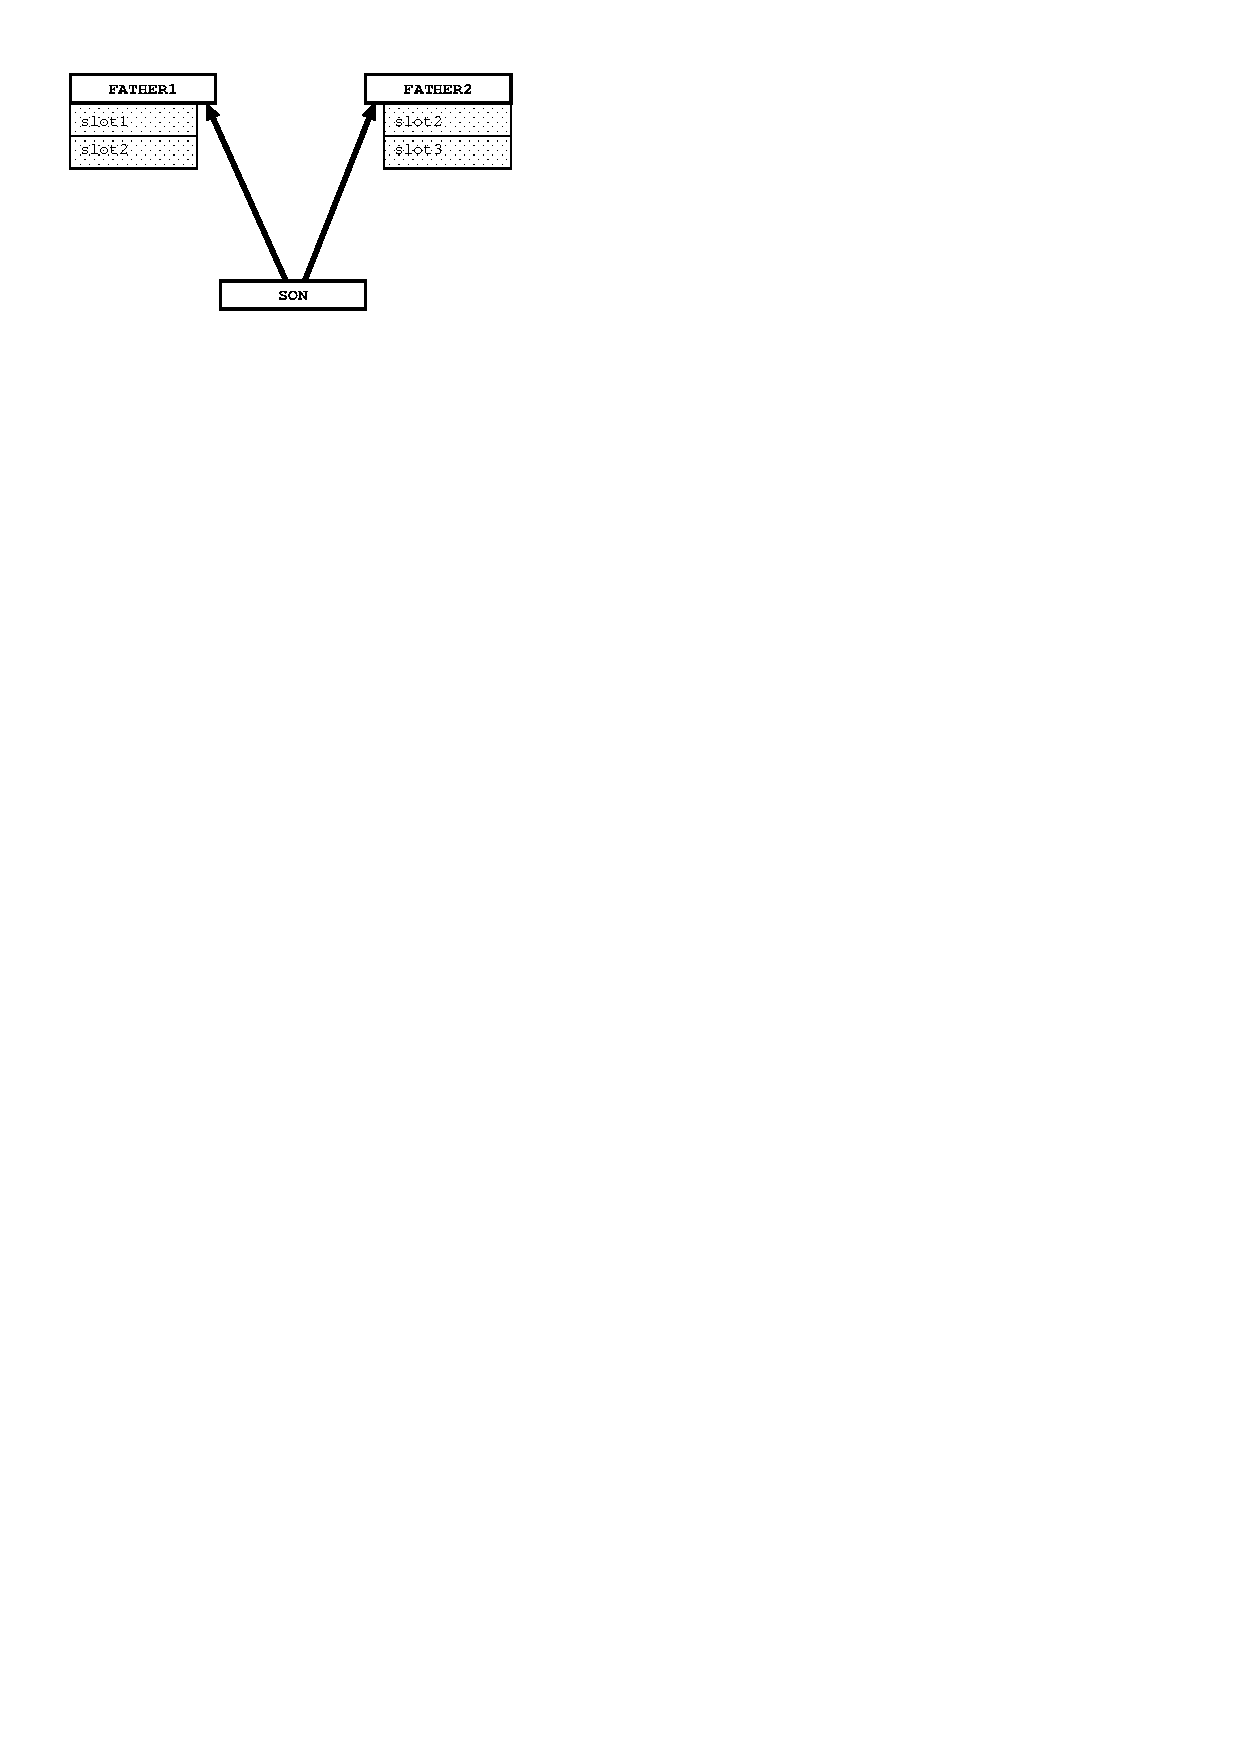
\includegraphics[scale=1.0]{figures/inherit_figure}
\end{center}

{\bf{}Section Header}
  + {\bf{}name}     := {\sc{}son};          

{\bf{}Section Inherit}
  - {\bf{}parent1}:{\sc{}father1} := {\sc{}father1};
  - {\bf{}parent2}:{\sc{}father2} := {\sc{}father2};\\

{\bf{}Section Header}
  + {\bf{}name}     := {\sc{}test};          

{\bf{}Section Public}
  - {\bf{}main} :=
  ( + object_son:{\sc{}son};
    object_son := {\sc{}son}.clone;
    object_son.{\bf{}slot1};    // From {\sc{}father1}
    object_son.{\bf{}slot2};    // From {\sc{}father1}
    object_son.{\bf{}slot3};    // From {\sc{}father2}
  );

\end{alltt}
\index{Slot, redefinition}
You can also redefine slots in the sons. Slot must follow the same typing profile as its parent (for parameters and result, see also {\ref{language_reference:type_names:invariant} page \pageref{language_reference:type_names:invariant}}) but you can change the kind of slot ({\bf{}+}, {\bf{}-} and {\bf{}Expanded}).

\begin{alltt}
{\bf{}Section Header}
  + {\bf{}name}     := {\sc{}father1};          

{\bf{}Section Public}
  + {\bf{}slot1} v:{\sc{}integer} :{\sc{}integer} <- /* \ldots */
  + {\bf{}slot2} <- /* \ldots */\\

{\bf{}Section Header}
  + {\bf{}name}     := {\sc{}father2};          

{\bf{}Section Public}
  + {\bf{}slot2} <- /* \ldots */
  + {\bf{}slot3} t:{\sc{}integer} <- /* \ldots */\\

{\bf{}Section Header}
  + {\bf{}name}     := {\sc{}son};          

{\bf{}Section Inherit}
  - {\bf{}parent1}:{\sc{}father1} := {\sc{}father1};
  - {\bf{}parent2}:{\sc{}father2} := {\sc{}father2};
{\bf{}Section Public}
  - {\bf{}slot1} v:{\sc{}integer} :{\sc{}integer} <- /* \ldots */  // {\bf{}slot1} is now shared

  + {\bf{}slot3} t:{\sc{}integer} <- /* \ldots */\\

{\bf{}Section Header}
  + {\bf{}name}     := {\sc{}test};          

{\bf{}Section Public}
  - {\bf{}main} :=
  ( + object_son:{\sc{}son};
    object_son := {\sc{}son}.clone;
    object_son.{\bf{}slot1} 4.print;    // From {\sc{}son}  (redefinition)
    object_son.{\bf{}slot2};            // From {\sc{}father1}
    object_son.{\bf{}slot3} 5;          // From {\sc{}son}  (redefinition)
  );
\end{alltt}

The name of the inheritance slot doesn't matter. We often named it "parent" but it's for more visibility than anything, it's not a reserved keyword.
But it's mandatory to be precise about the type of the parent, as for any data slot.\\

As every slot in Lisaac, inheritance slots have 3 different behaviours.\\
%.........................................................
\subsubsection{Shared inheritance}
\label{language_reference:section_identifiers:inherit_section:shared_inheritance}
%.........................................................
%
\index{Inheritance, shared}
A parent can be defined with the the {\bf{} -} symbol:
\begin{alltt}
{\bf{}Section Inherit}
  - {\bf{} parent}:{\sc{}father} := {\sc{}father};
\end{alltt}
In this case every clone of the object share the same parent object. If a son object change its parent, every clone of this son have their parent changed.
\begin{center}
Object {\sc{}father}
\end{center}
\begin{alltt} 
{\bf{}Section Header}
  + {\bf{}name}     := {\sc{}father};          

{\bf{}Section Public}
  + {\bf{}x}    :{\sc{}integer};
  - {\bf{}inc\_x} <- ( x := x + 1; );
  - {\bf{}count}:{\sc{}integer};
  - {\bf{}inc\_count} <- ( count := count + 1; );
\end{alltt}
\begin{center}
Object {\sc{}son}
\end{center}
\begin{alltt} 
{\bf{}Section Header}
  + {\bf{}name}     := {\sc{}son};          

{\bf{}Section Inherit}
  - {\bf{}parent}:{\sc{}father} := {\sc{}father};
{\bf{}Section Public}
  - {\bf{}change\_parent} p:{\sc{}father} <- ( parent := p; );
\end{alltt}
\begin{center}
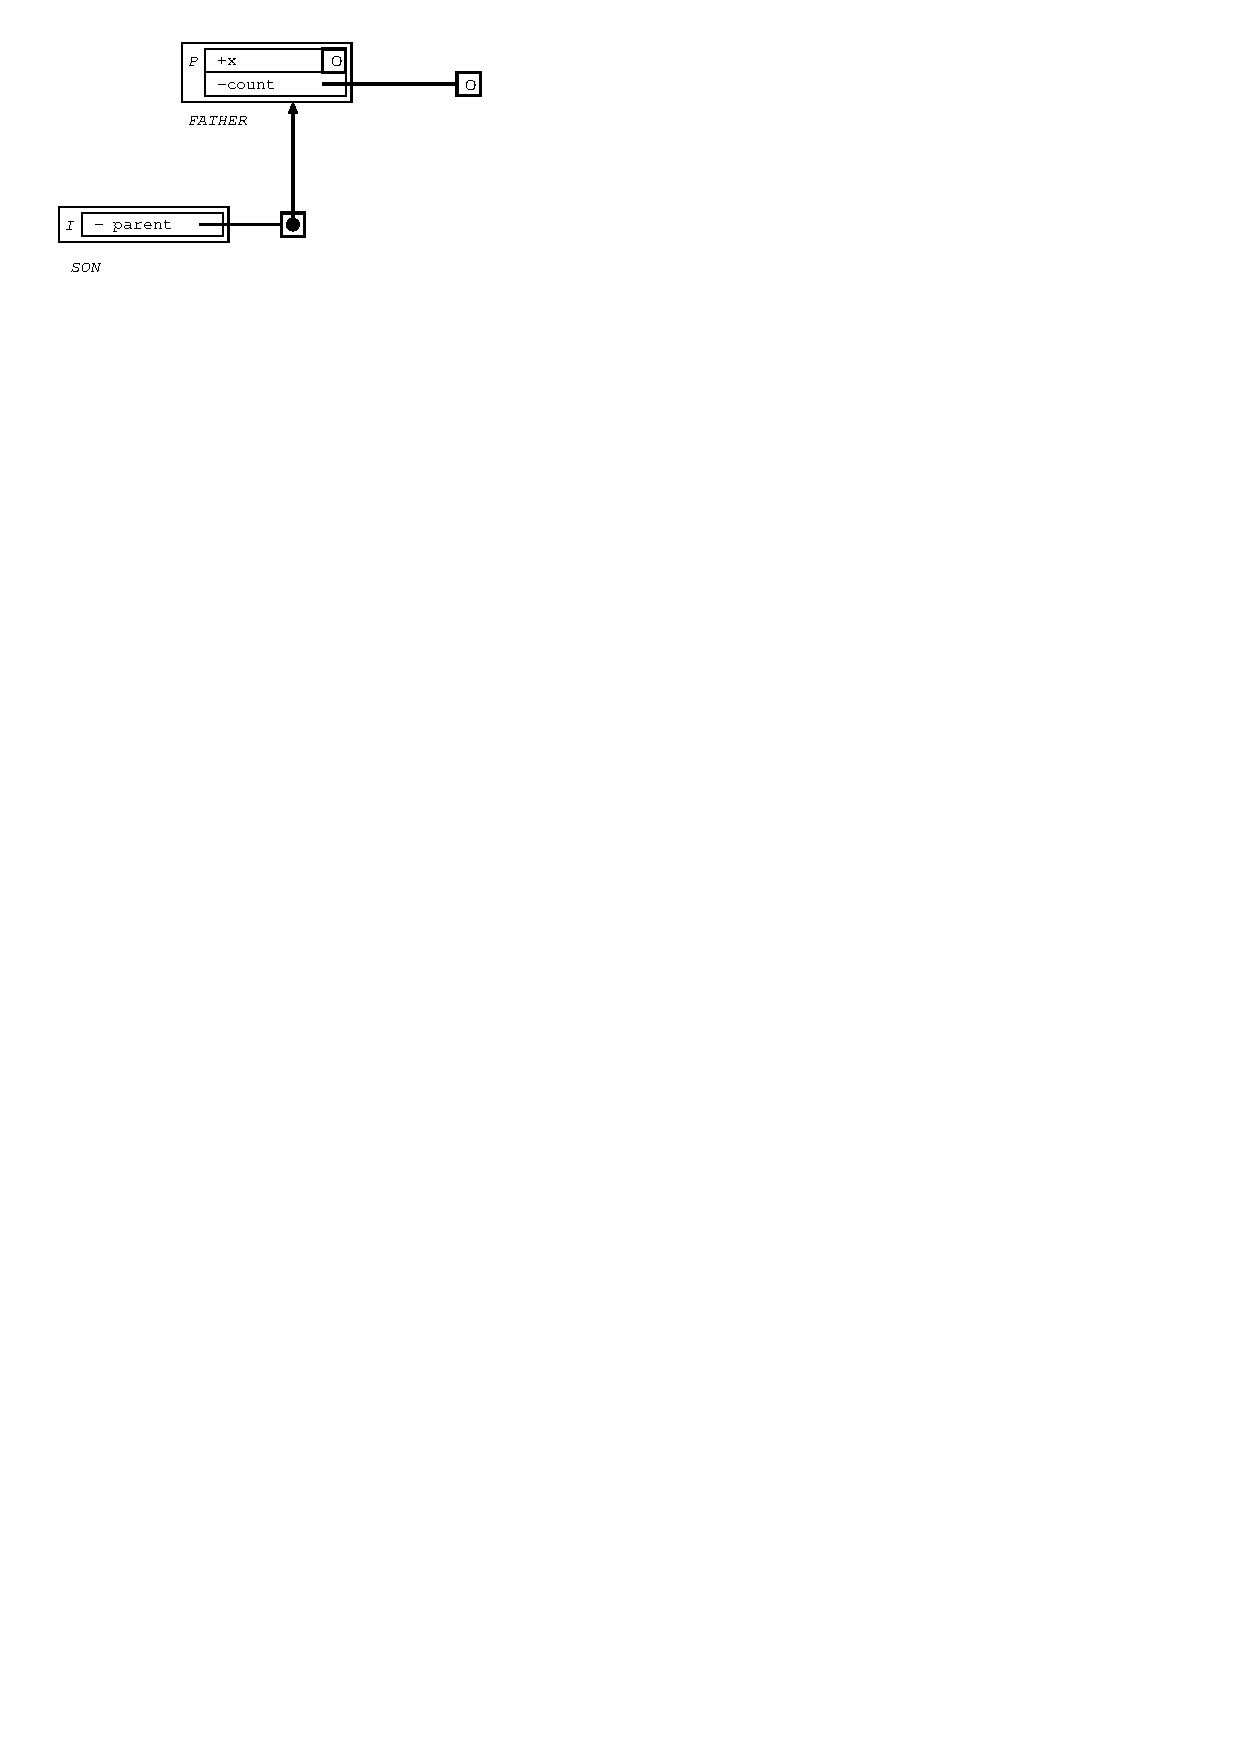
\includegraphics[scale=1.0]{figures/inherit_minus_0}
\end{center}

\begin{alltt}
  new\_son := {\sc{}son}.{\bf{}clone};
\end{alltt}
\begin{center}
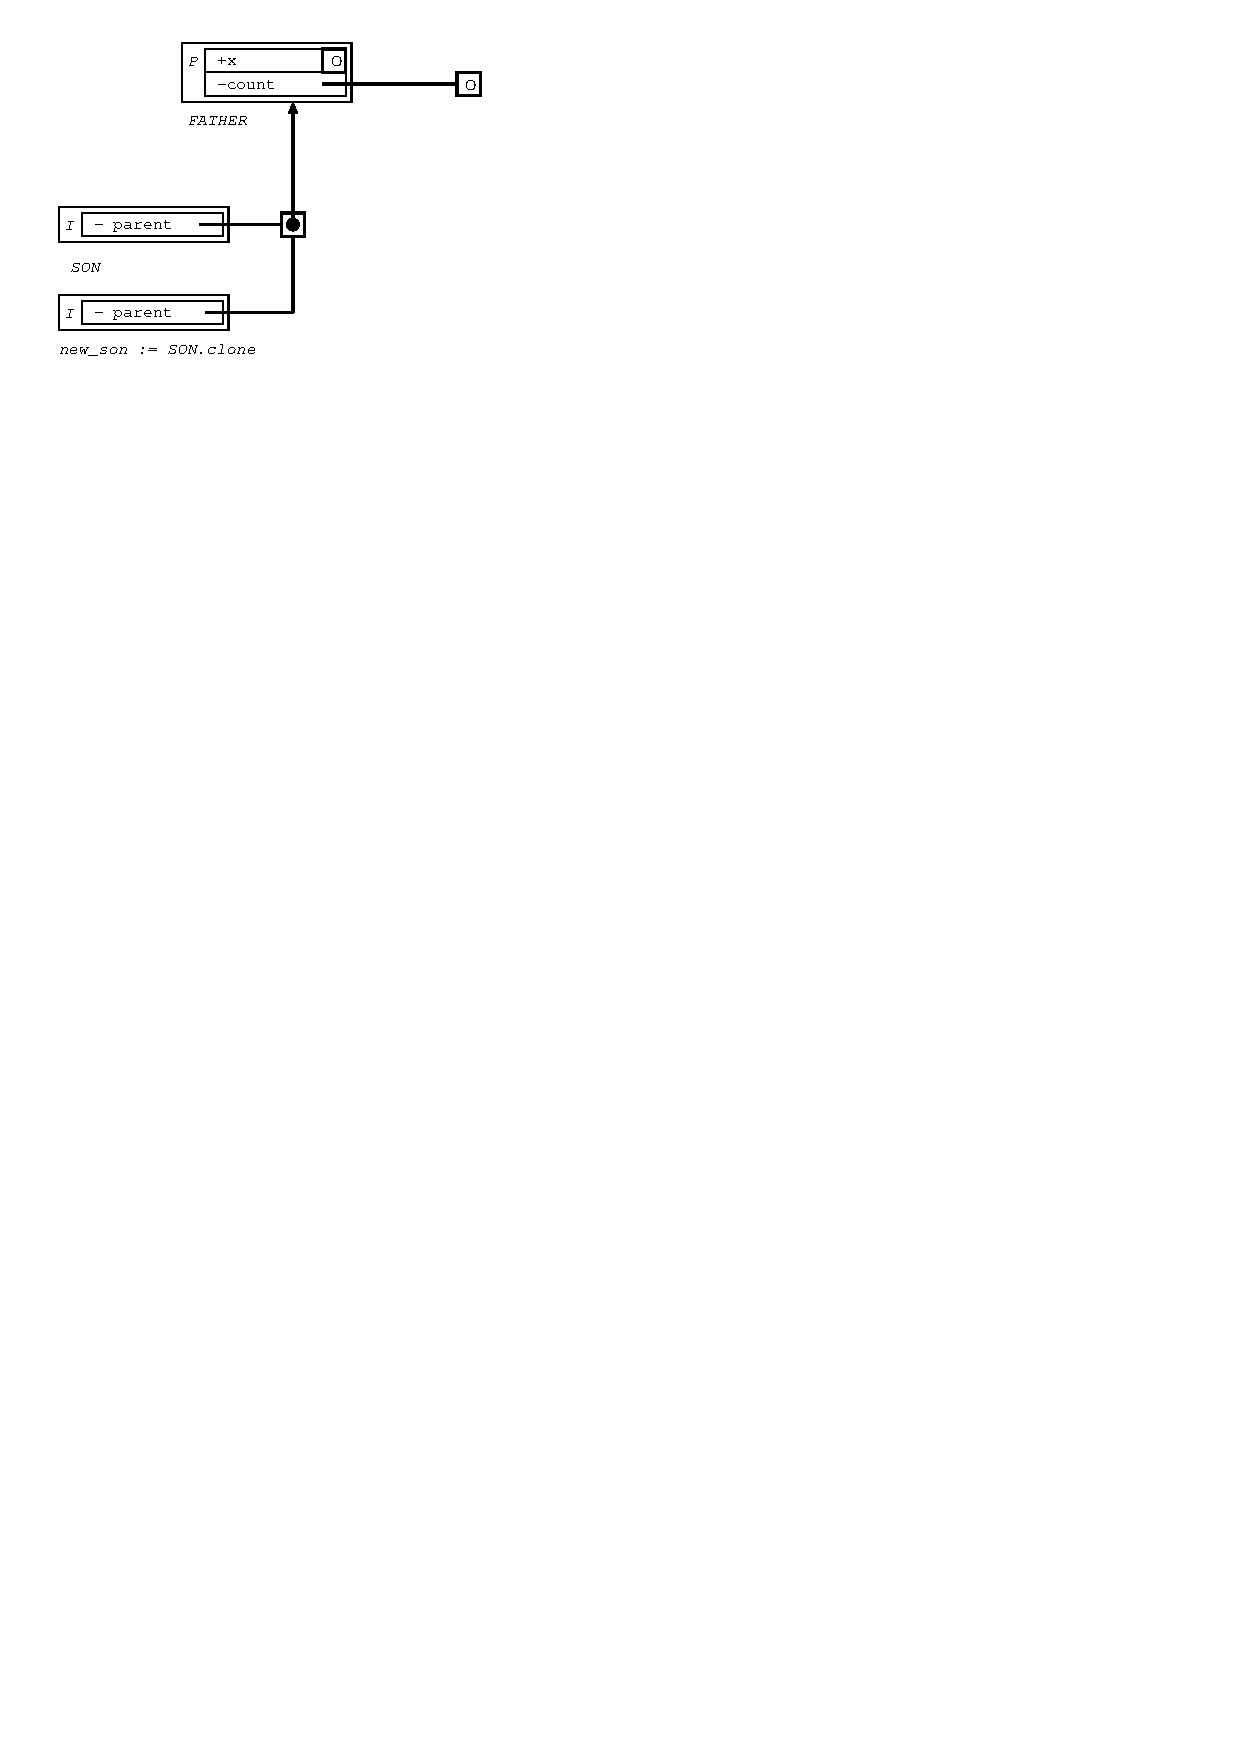
\includegraphics[scale=1.0]{figures/inherit_minus_1} 
\end{center}

\begin{alltt}
  new\_son.{\bf{}inc\_x};
  new\_son.{\bf{}inc\_count};
\end{alltt}
\begin{center}
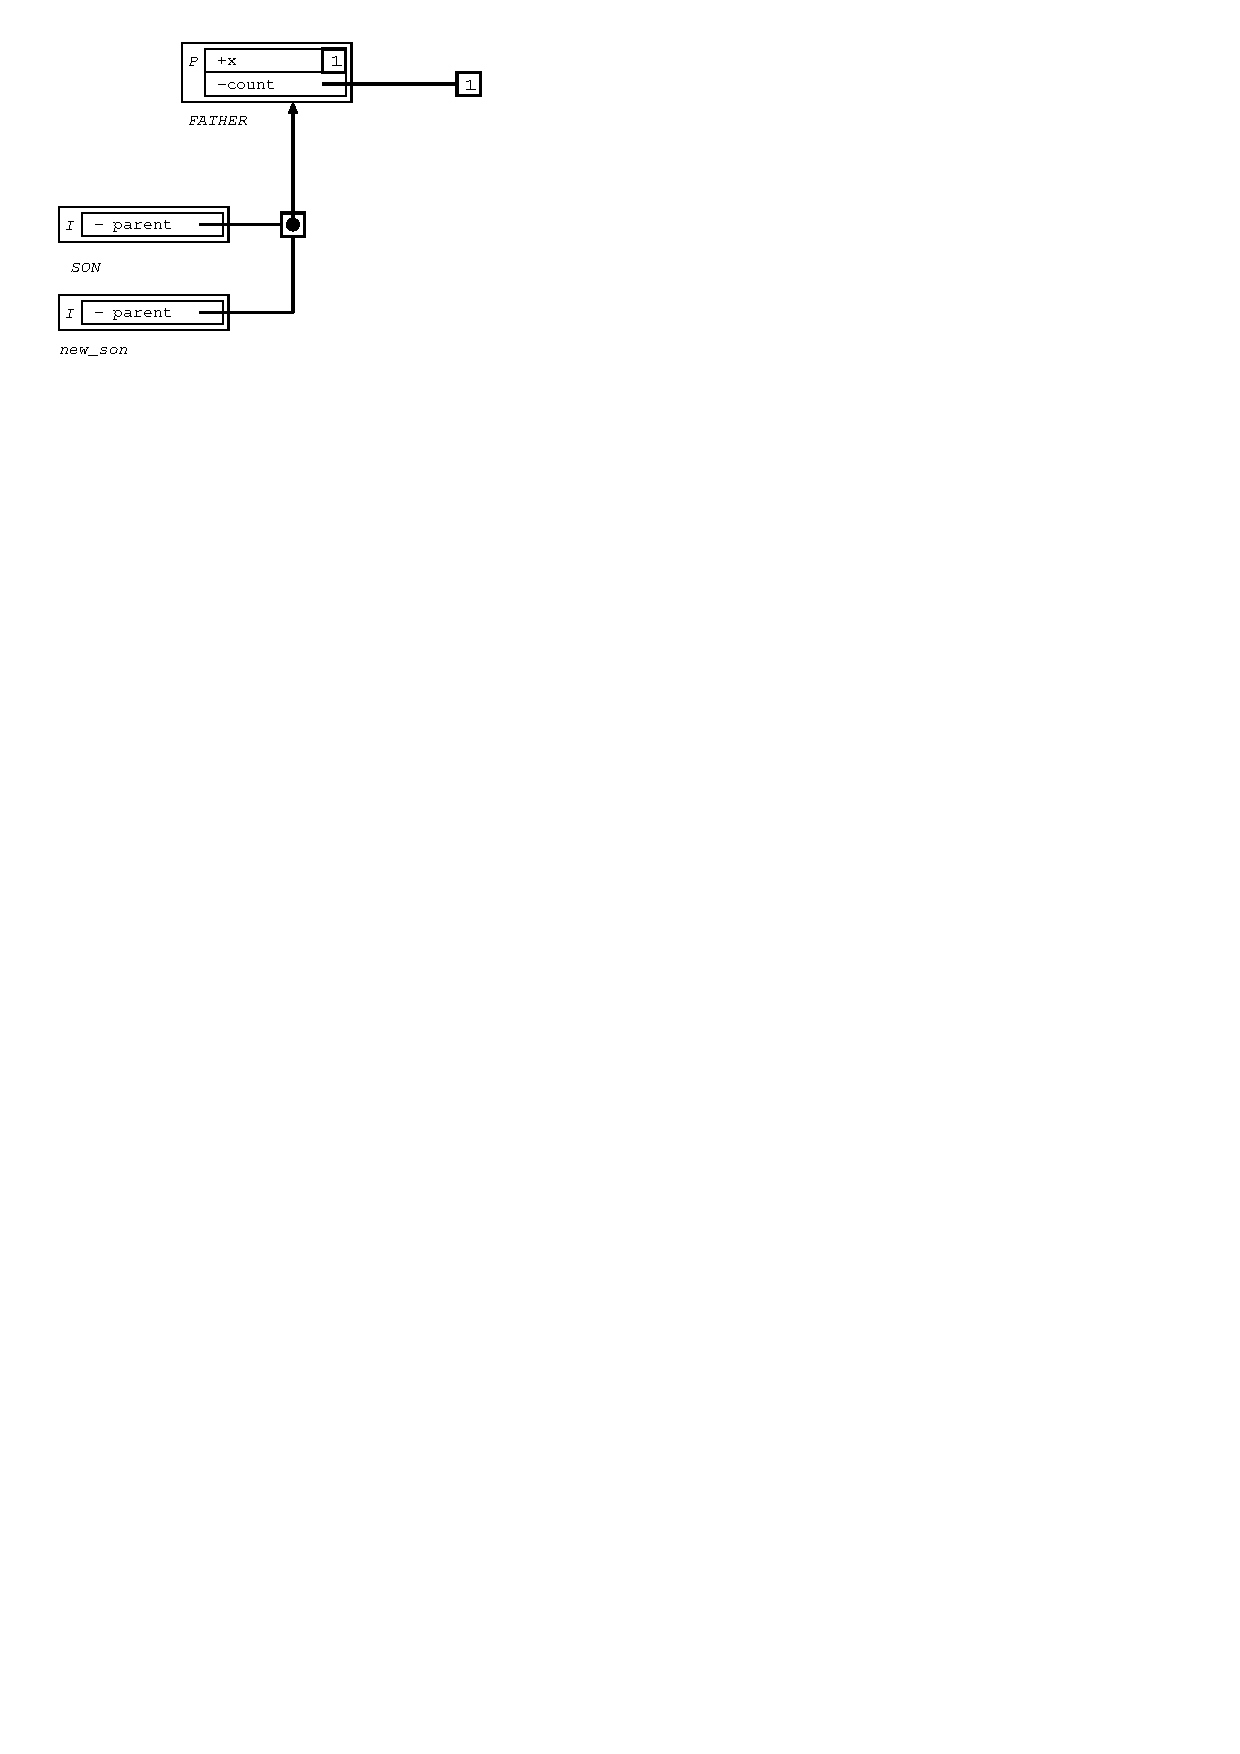
\includegraphics[scale=1.0]{figures/inherit_minus_2} 
\end{center}

\begin{alltt}
  new\_son.{\bf{}change\_parent} ({\sc{}father}.{\bf{}clone});
\end{alltt}
\begin{center}
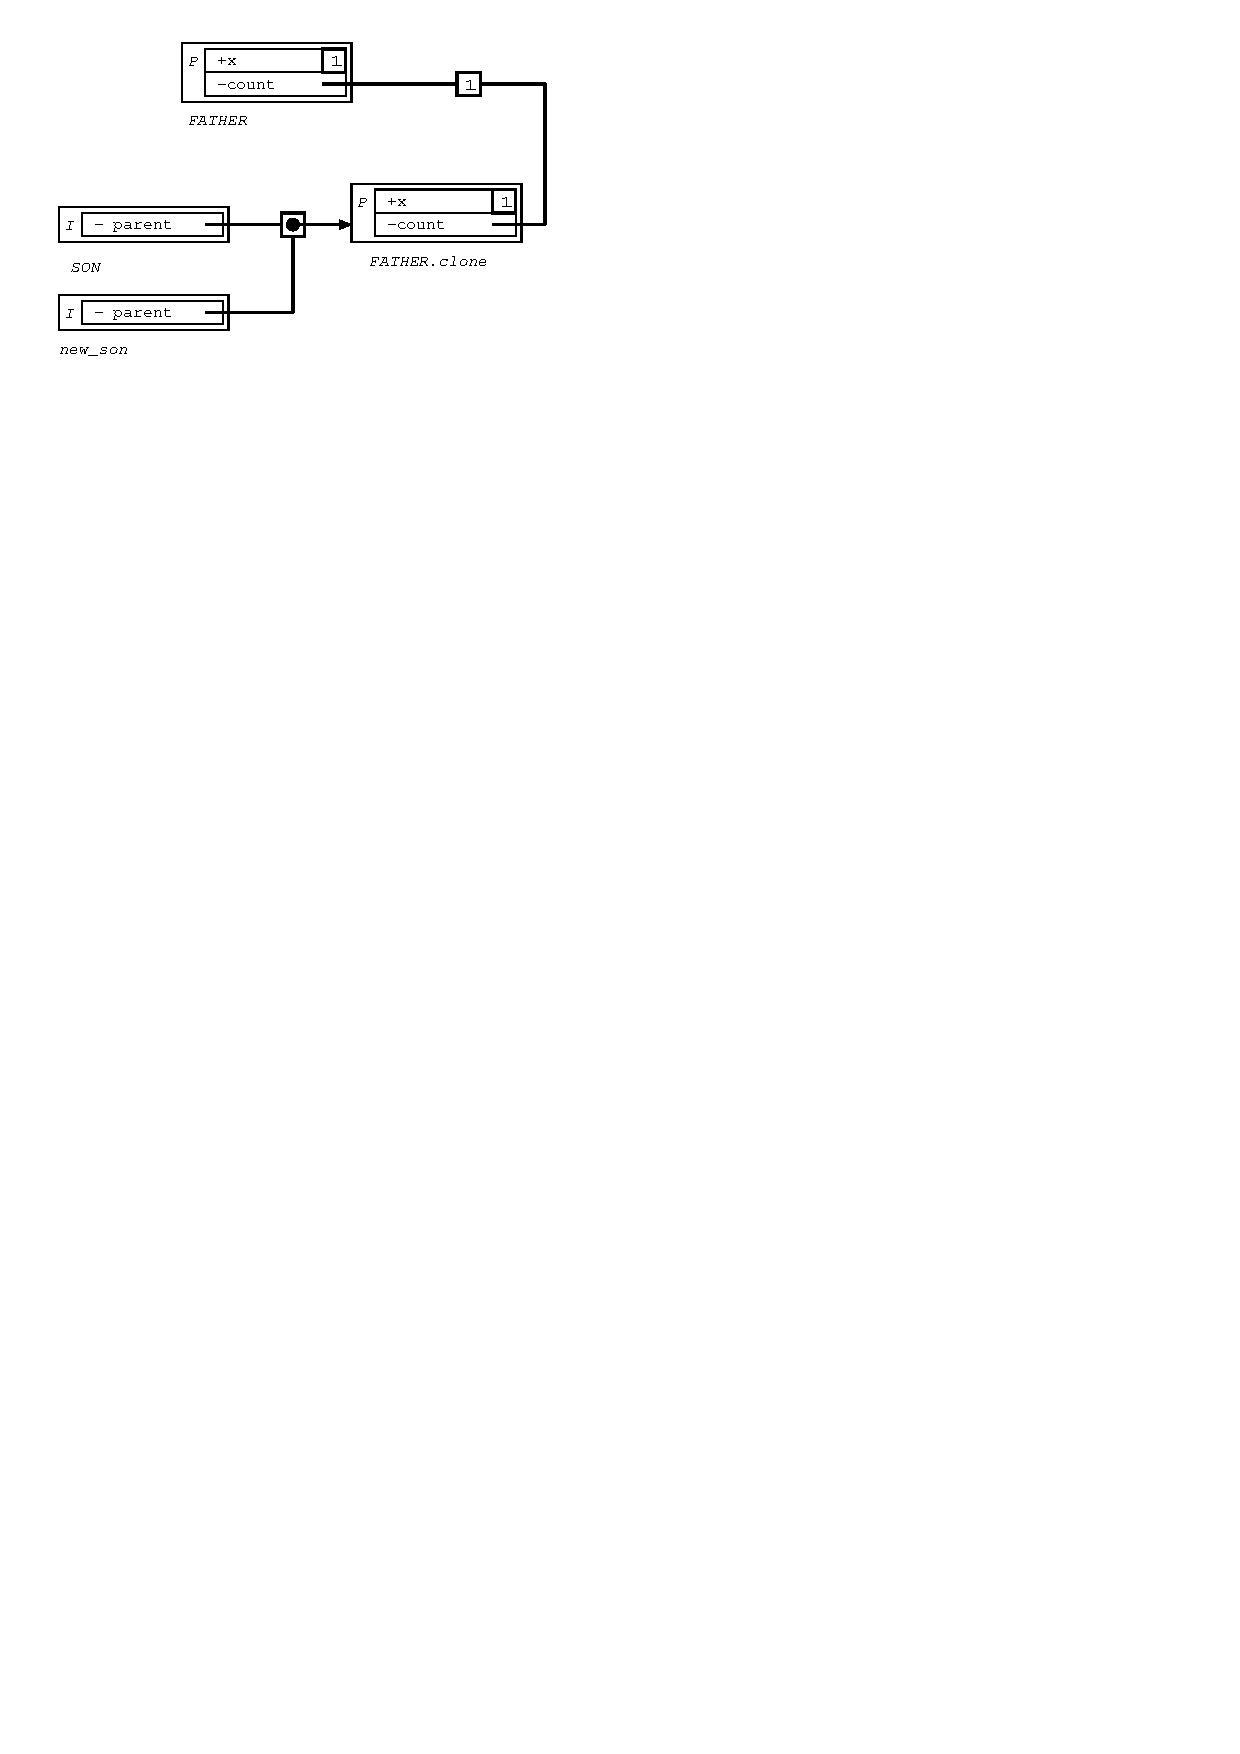
\includegraphics[scale=1.0]{figures/inherit_minus_3} 
\end{center}

\begin{alltt}
  new\_son.{\bf{}inc\_x};
  new\_son.{\bf{}inc\_count};
\end{alltt}
\begin{center}
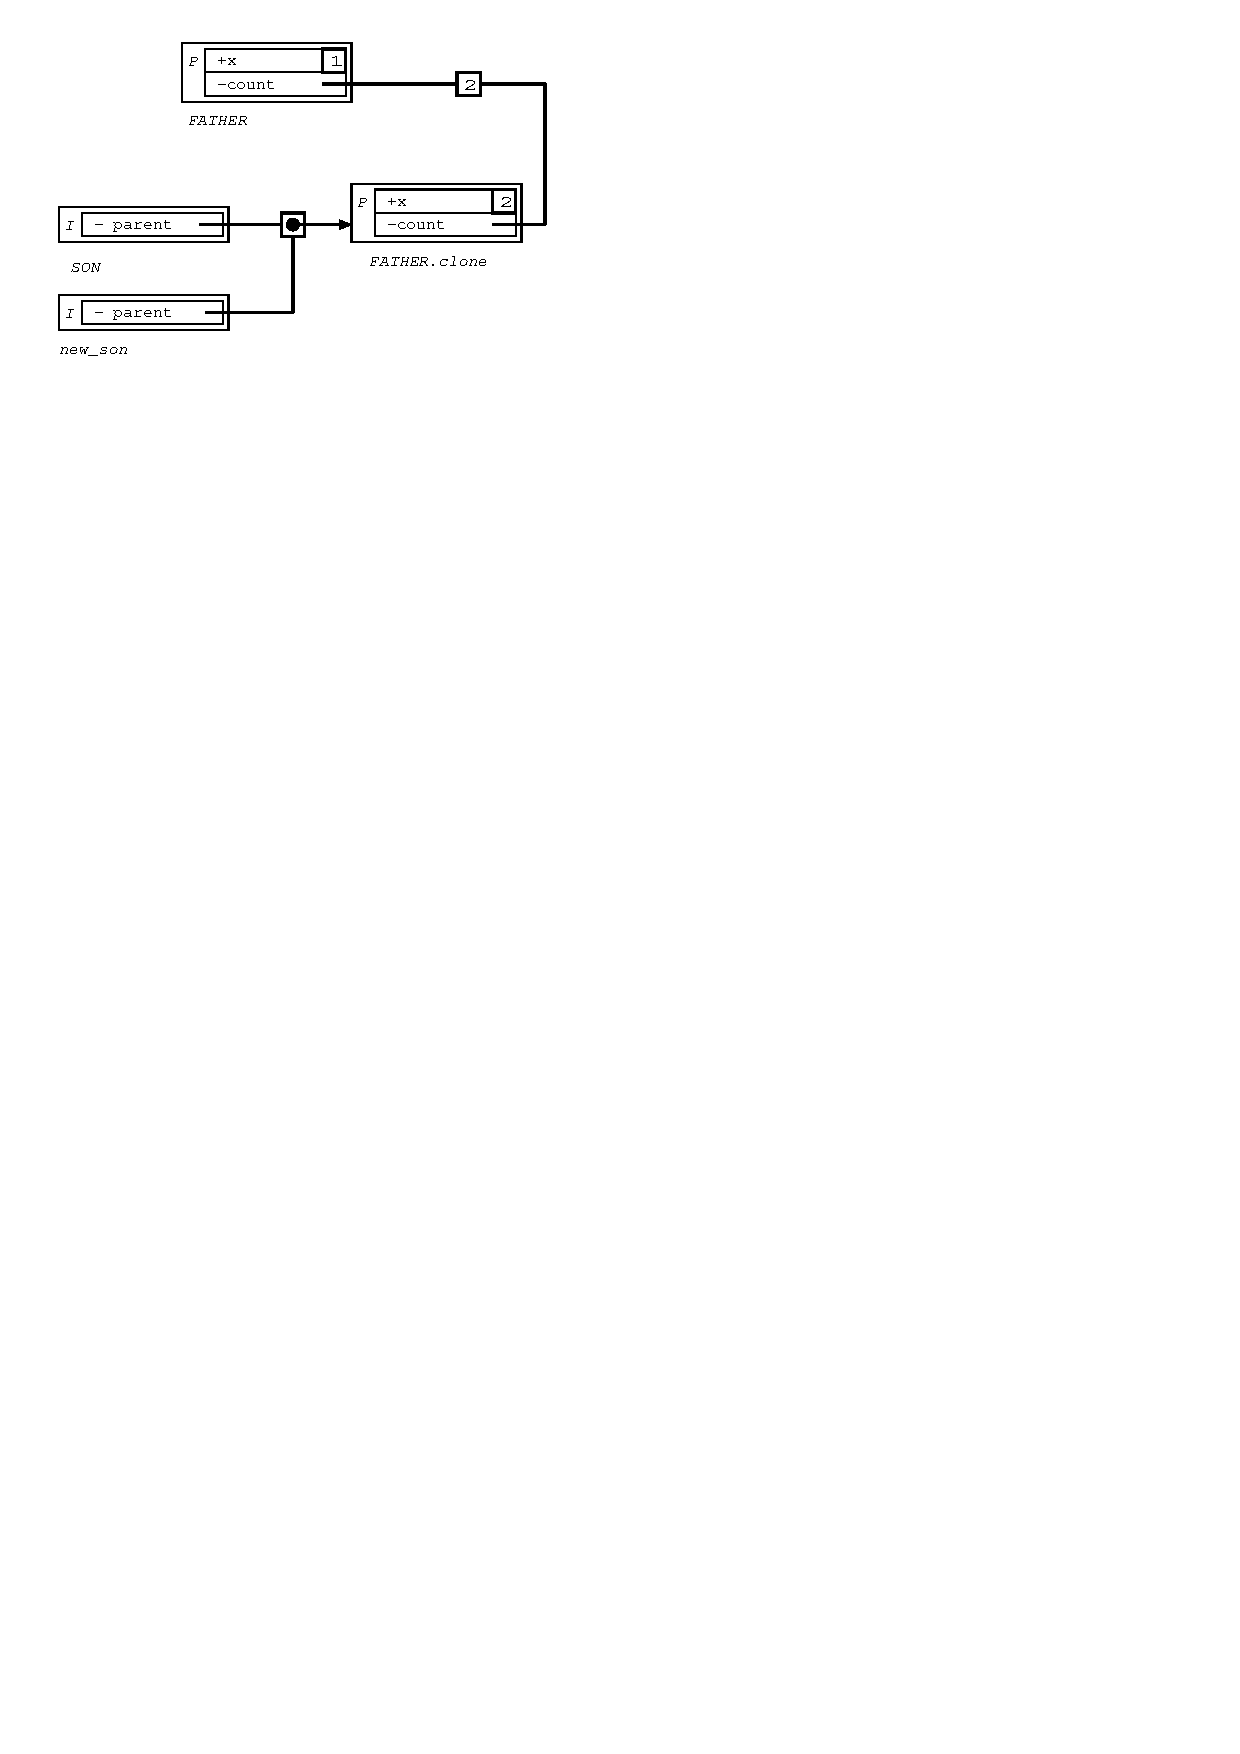
\includegraphics[scale=1.0]{figures/inherit_minus_4} 
\end{center}
%.........................................................
\subsubsection{Non shared inheritance}
\label{language_reference:section_identifiers:inherit_section:non_shared_inheritance}
%.........................................................
%
\index{Inheritance, non shared}
A parent can be defined with the the {\bf{} +} symbol:
\begin{alltt}
{\bf{}Section Inherit}
  + {\bf{} parent}:{\sc{}father} := {\sc{}father};
\end{alltt}
In this case every clone of the object share the same parent object at its creation. If a son object change its parent, other clones of this son haven't got their parents changed.
\begin{center}
Object {\sc{}father}
\end{center}
\begin{alltt} 
{\bf{}Section Header}
  + {\bf{}name}     := {\sc{}father};          

{\bf{}Section Public}
  + {\bf{}x}    :{\sc{}integer};
  - {\bf{}inc\_x} <- ( x := x + 1; );
  - {\bf{}count}:{\sc{}integer};
  - {\bf{}inc\_count} <- ( count := count + 1; );
\end{alltt}
\begin{center}
Object {\sc{}son}
\end{center}
\begin{alltt} 
{\bf{}Section Header}
  + {\bf{}name}     := {\sc{}son};          

{\bf{}Section Inherit}
  + {\bf{}parent}:{\sc{}father} := {\sc{}father};
{\bf{}Section Public}
  - {\bf{}change\_parent} p:{\sc{}father} <- ( parent := p; );
\end{alltt}
\begin{center}
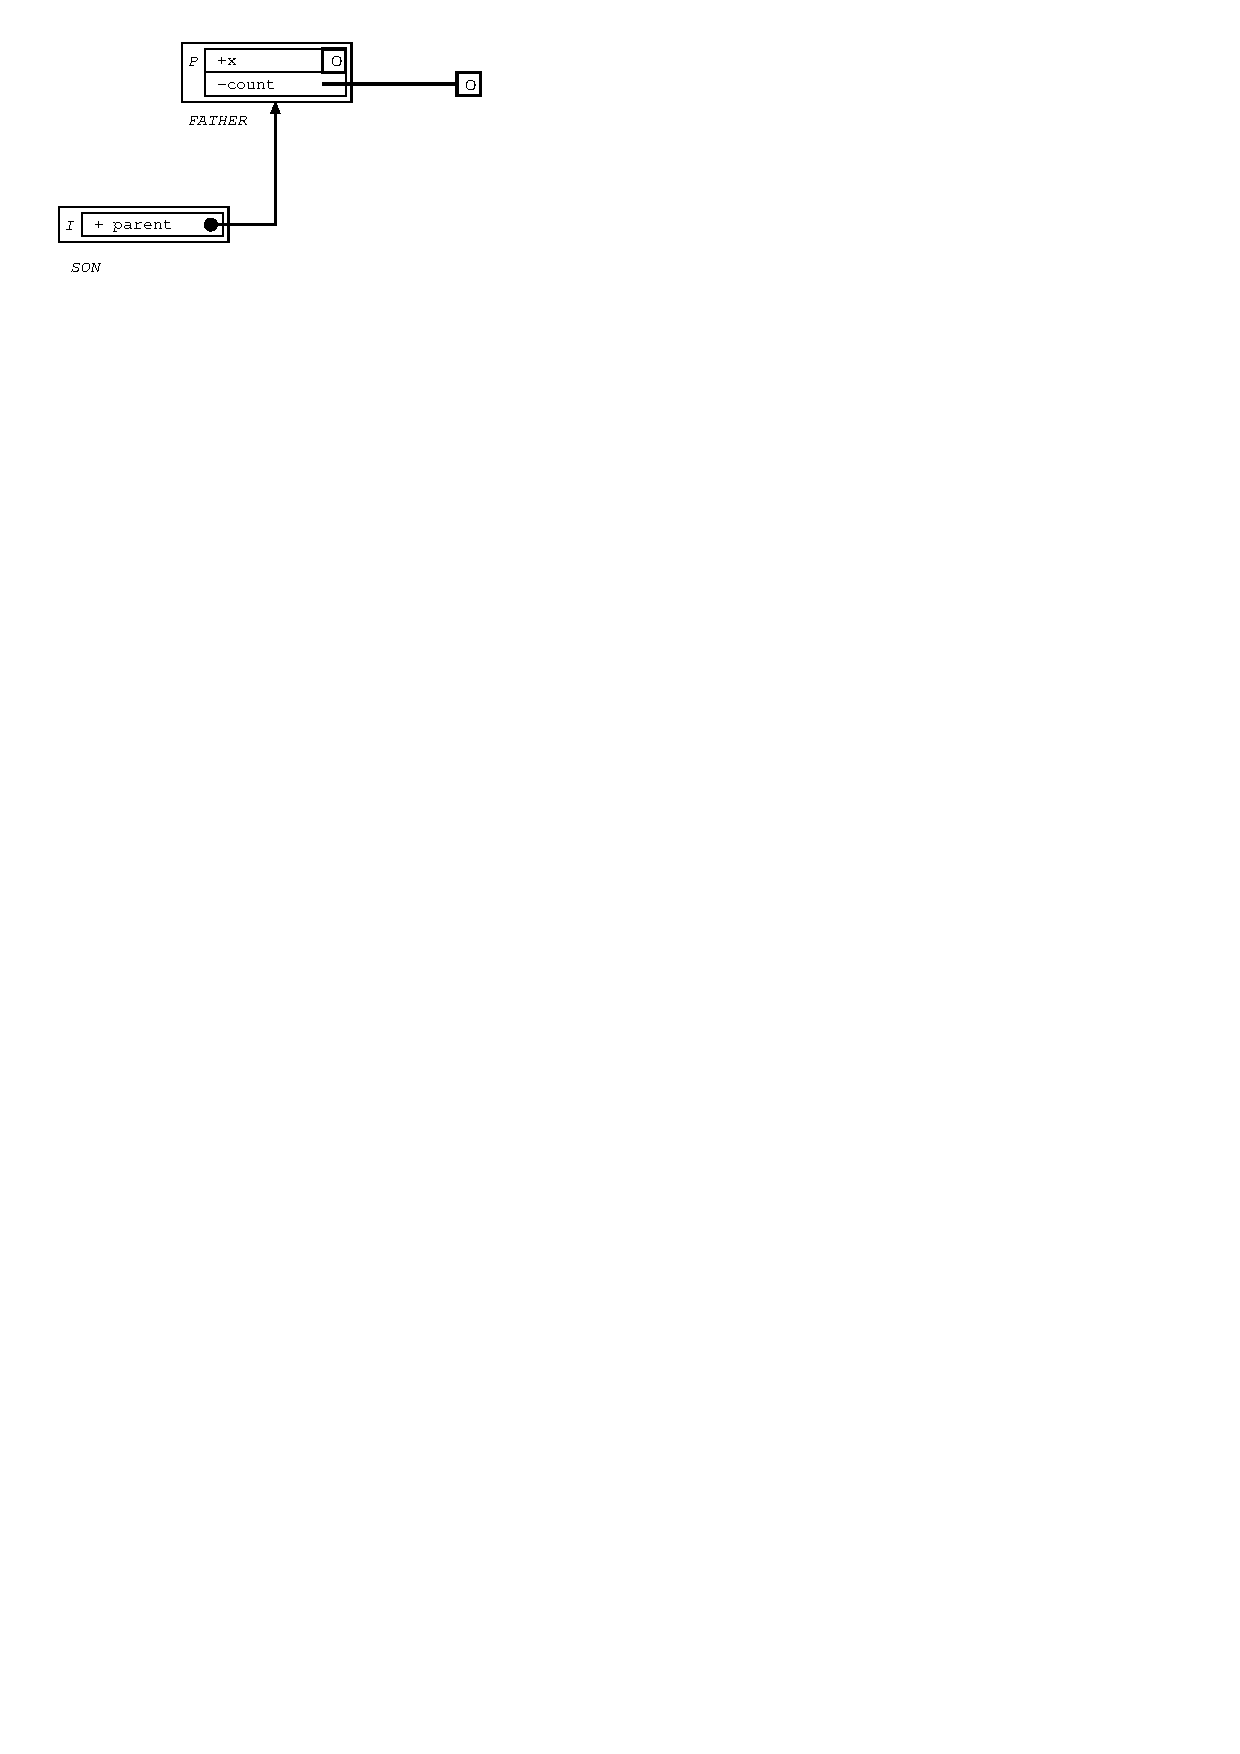
\includegraphics[scale=1.0]{figures/inherit_plus_0}
\end{center}

\begin{alltt}
  new\_son := {\sc{}son}.{\bf{}clone};
\end{alltt}
\begin{center}
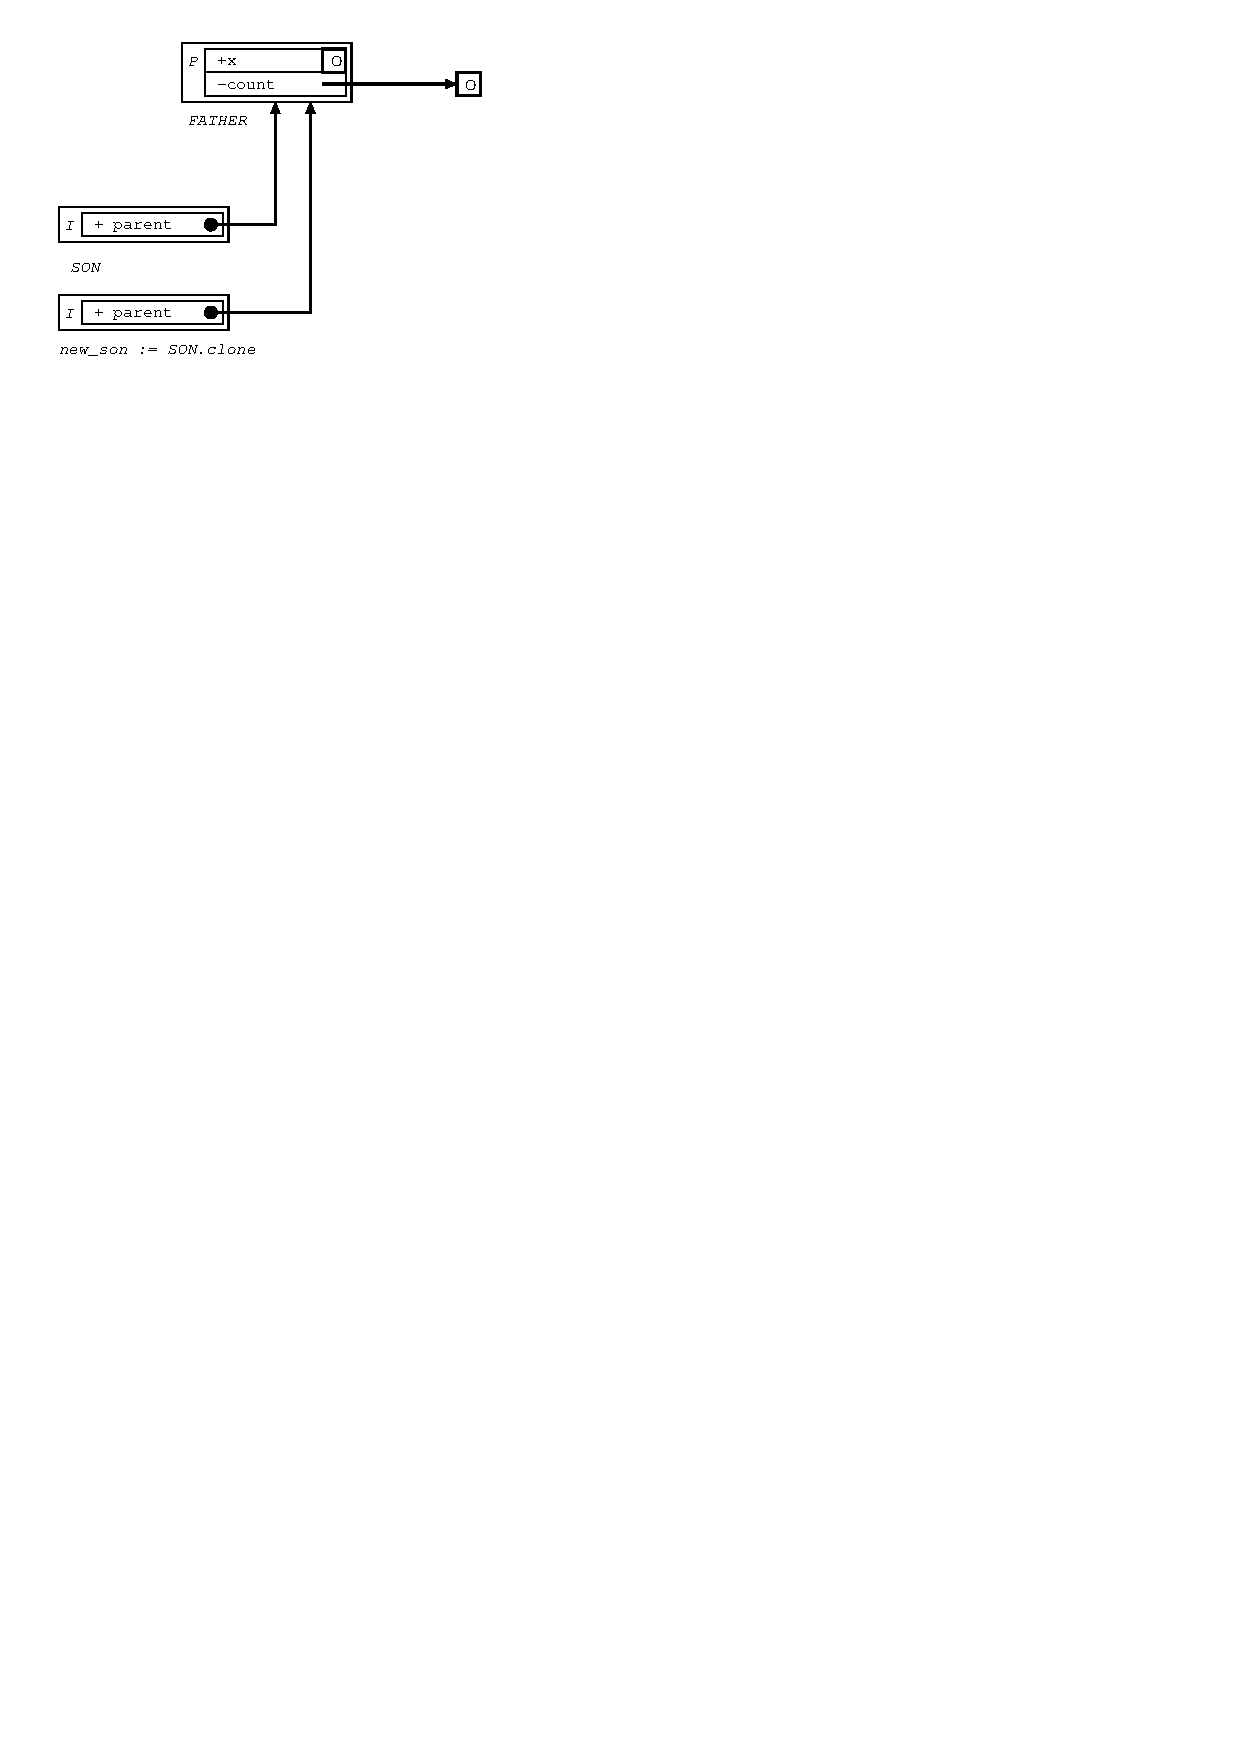
\includegraphics[scale=1.0]{figures/inherit_plus_1} 
\end{center}

\begin{alltt}
  new\_son.{\bf{}inc\_x};
  new\_son.{\bf{}inc\_count};
\end{alltt}
\begin{center}
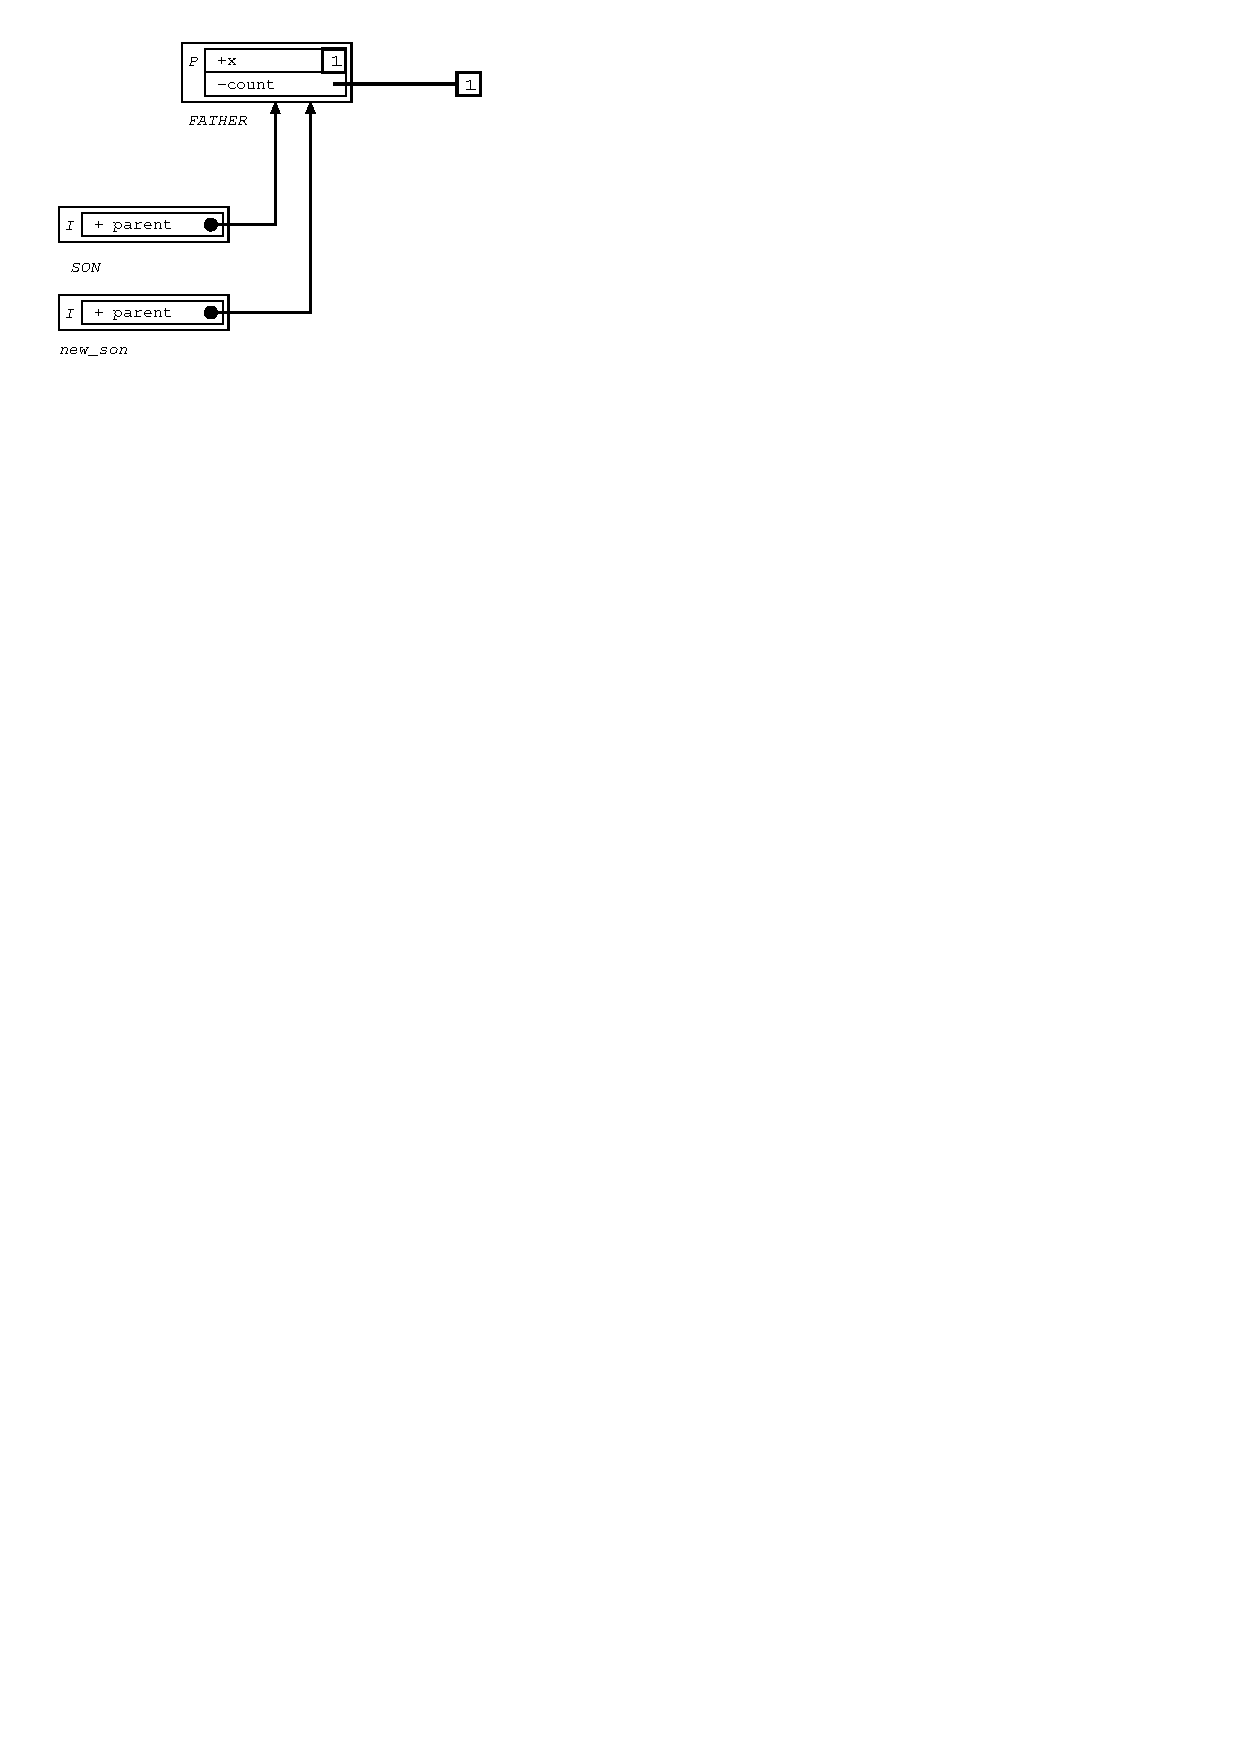
\includegraphics[scale=1.0]{figures/inherit_plus_2} 
\end{center}

\begin{alltt}
  new\_son.{\bf{}change\_parent} ({\sc{}father}.{\bf{}clone});
\end{alltt}
\begin{center}
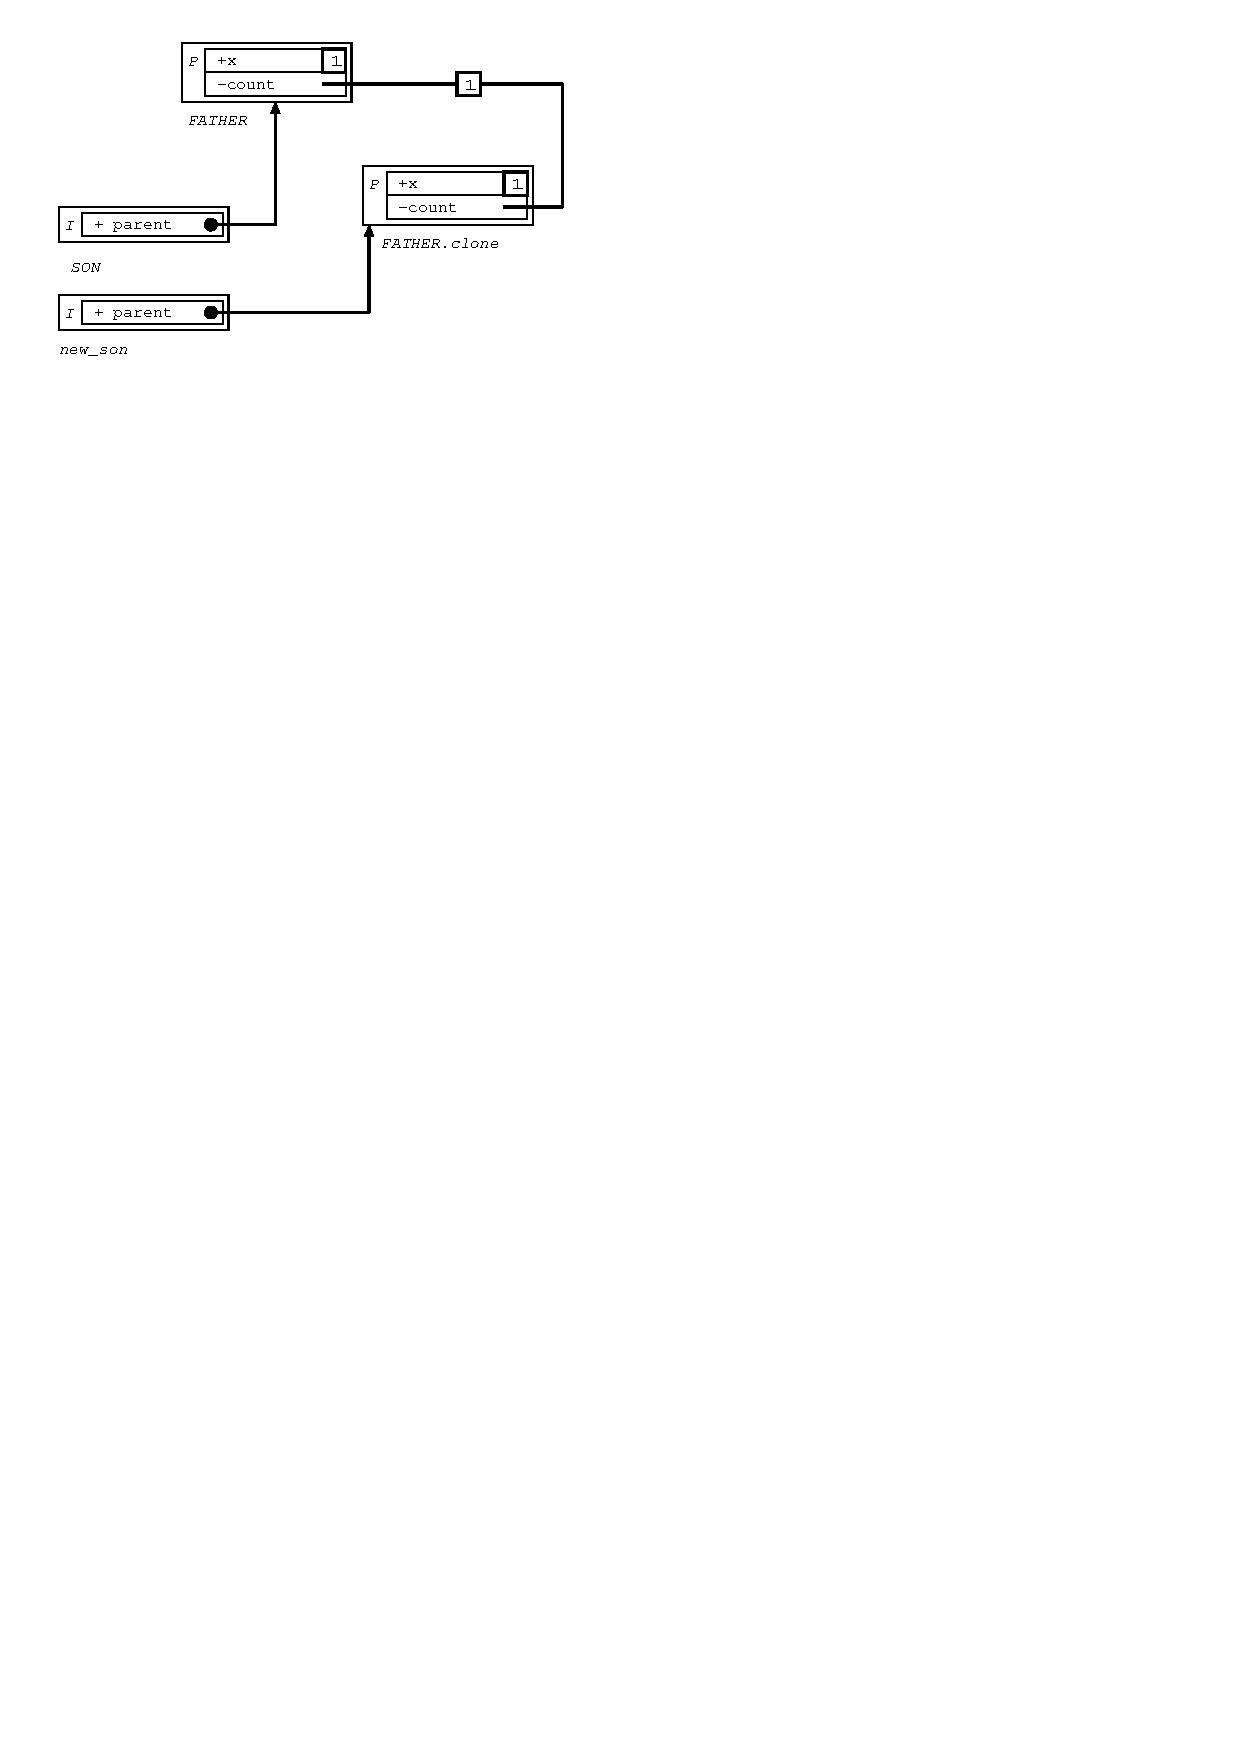
\includegraphics[scale=1.0]{figures/inherit_plus_3} 
\end{center}

\begin{alltt}
  new\_son.{\bf{}inc\_x};
  new\_son.{\bf{}inc\_count};
\end{alltt}
\begin{center}
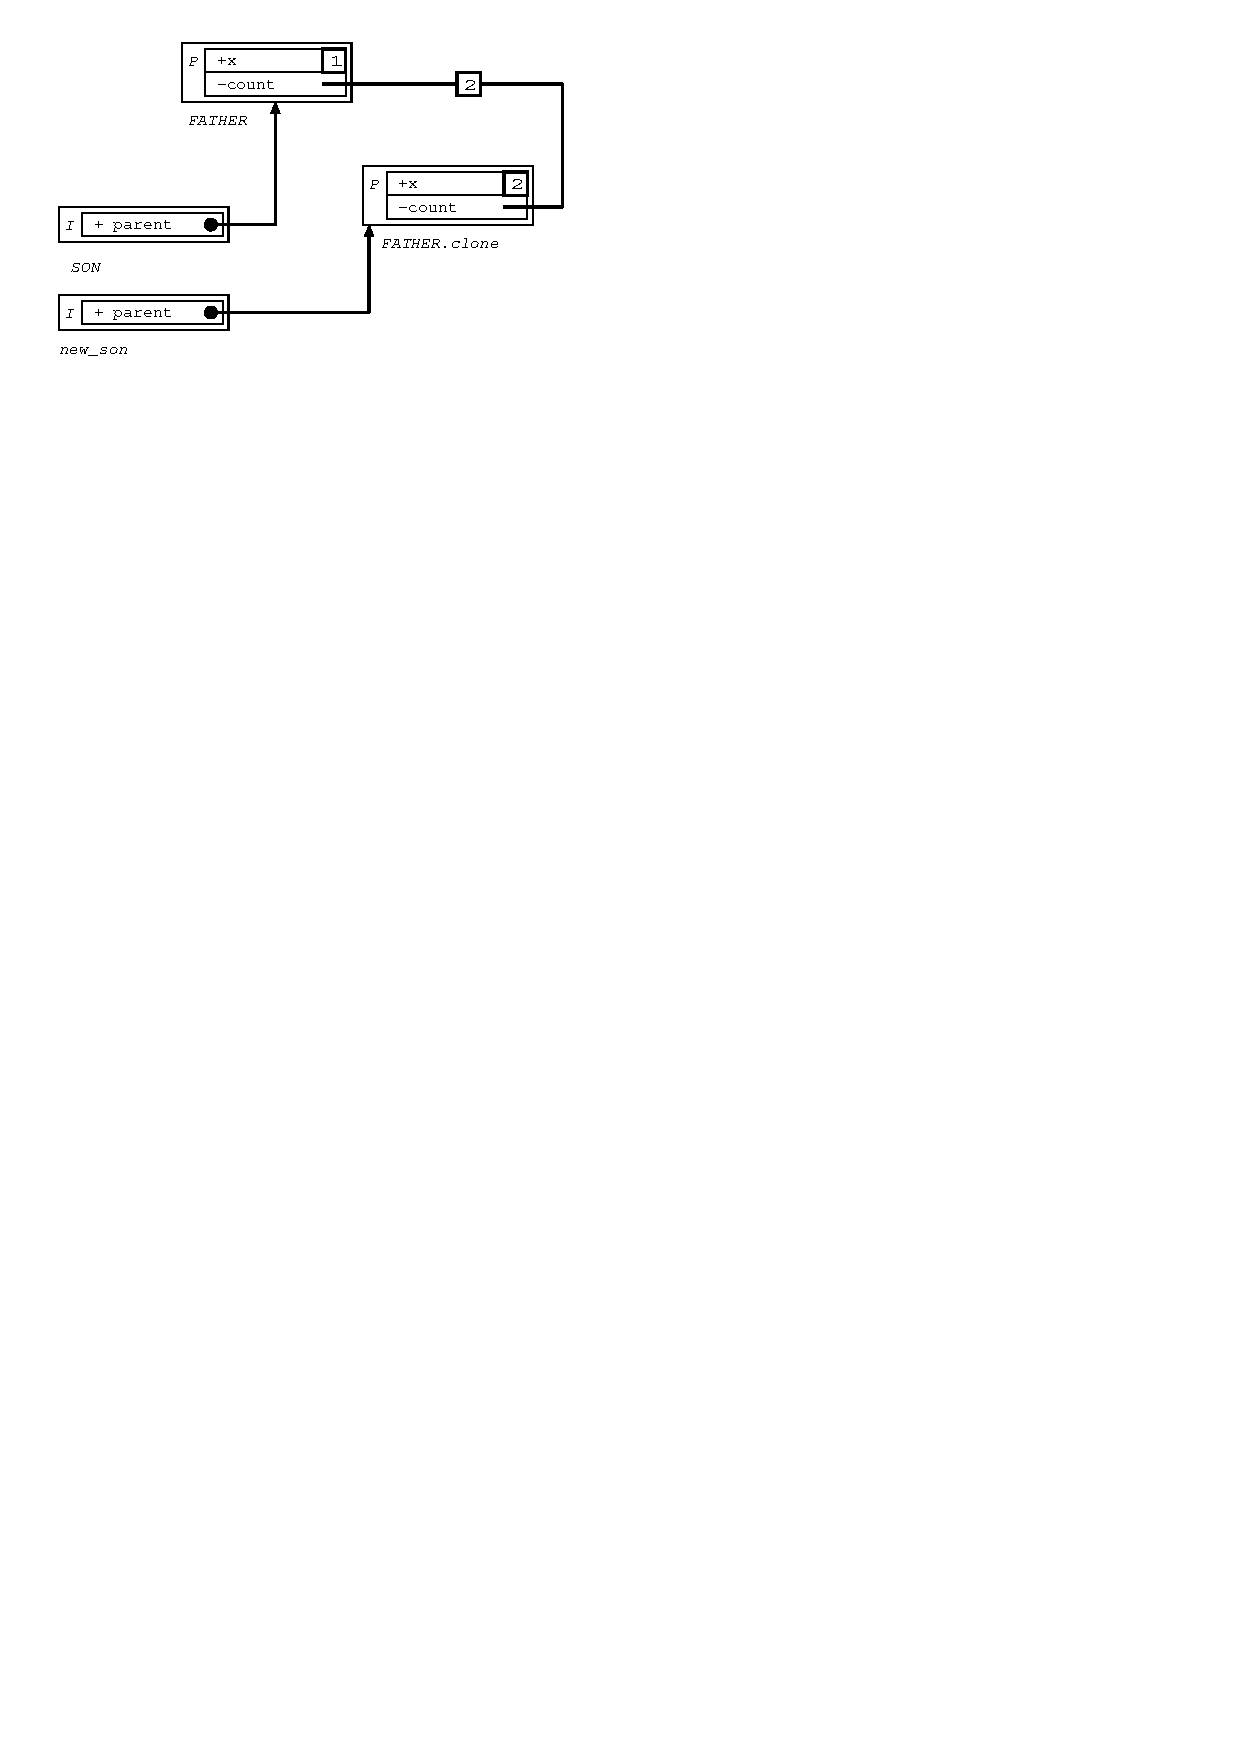
\includegraphics[scale=1.0]{figures/inherit_plus_4} 
\end{center}
%.........................................................
\subsubsection{Expanded inheritance}
\label{language_reference:section_identifiers:inherit_section:expanded_inheritance}
%.........................................................
%
\index{Inheritance, expanded}
A parent can be defined with the the {\bf{} +} symbol and the {\bf{}Expanded} keyword:
\begin{alltt}
{\bf{}Section Inherit}
  + {\bf{} parent}:{\bf{}Expanded} {\sc{}father};
\end{alltt}
\warning{} In this case, you don't have to affect the value of the parent.

You have an "auto-clone" for parents: each time you clone a son, you have the clone of its parents.
\begin{center}
Object {\sc{}father}
\end{center}
\begin{alltt} 
{\bf{}Section Header}
  + {\bf{}name}     := {\sc{}father};          

{\bf{}Section Public}
  + {\bf{}x}    :{\sc{}integer};
  - {\bf{}inc\_x} <- ( x := x + 1; );
  - {\bf{}count}:{\sc{}integer};
  - {\bf{}inc\_count} <- ( count := count + 1; );
\end{alltt}
\begin{center}
Object {\sc{}son}
\end{center}
\begin{alltt} 
{\bf{}Section Header}
  + {\bf{}name}     := {\sc{}son};          

{\bf{}Section Inherit}
  + {\bf{}parent}:{\bf{}Expanded} {\sc{}father};
{\bf{}Section Public}
  - {\bf{}change\_parent} p:{\sc{}father} <- ( parent := p; );
\end{alltt}
\begin{center}
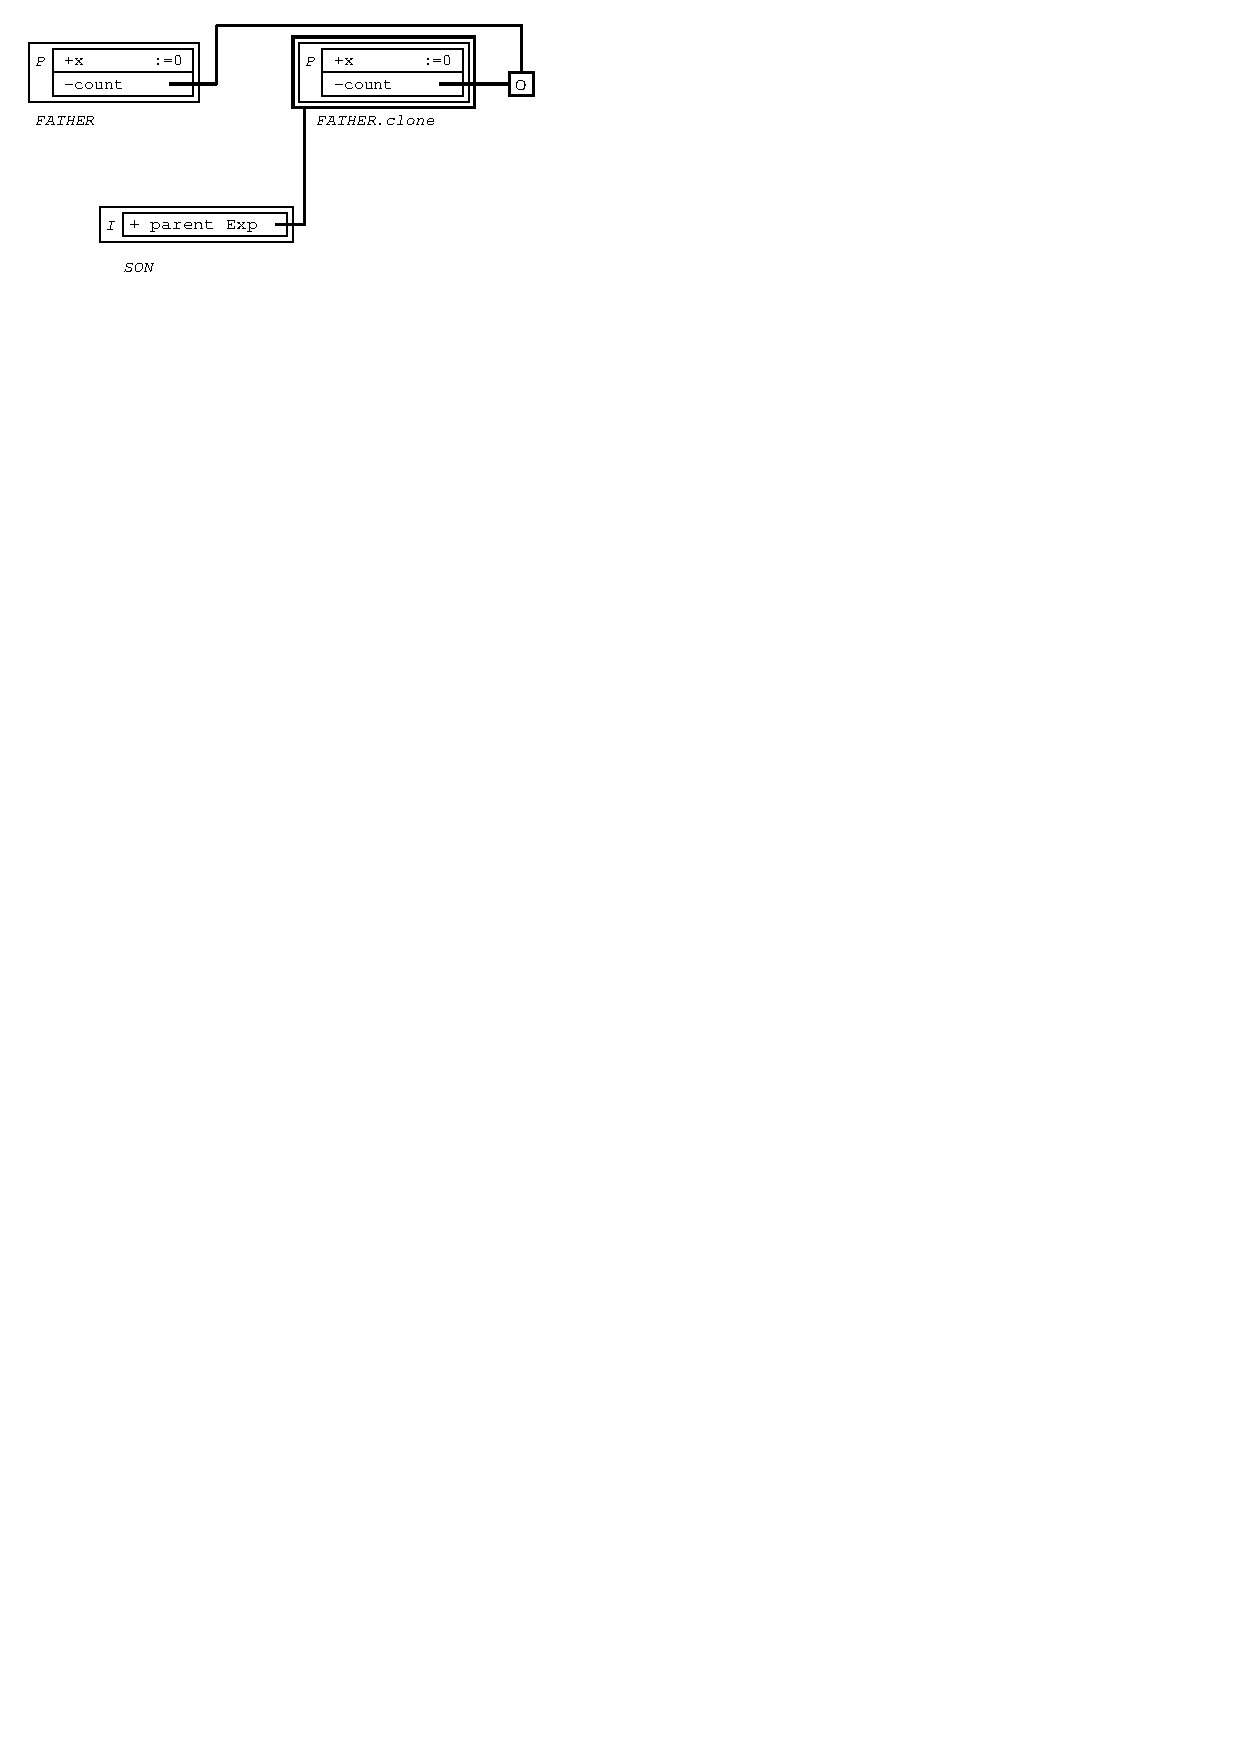
\includegraphics[scale=1.0]{figures/inherit_expanded_0}
\end{center}

\begin{alltt}
  new\_son := {\sc{}son}.{\bf{}clone};
\end{alltt}
\begin{center}
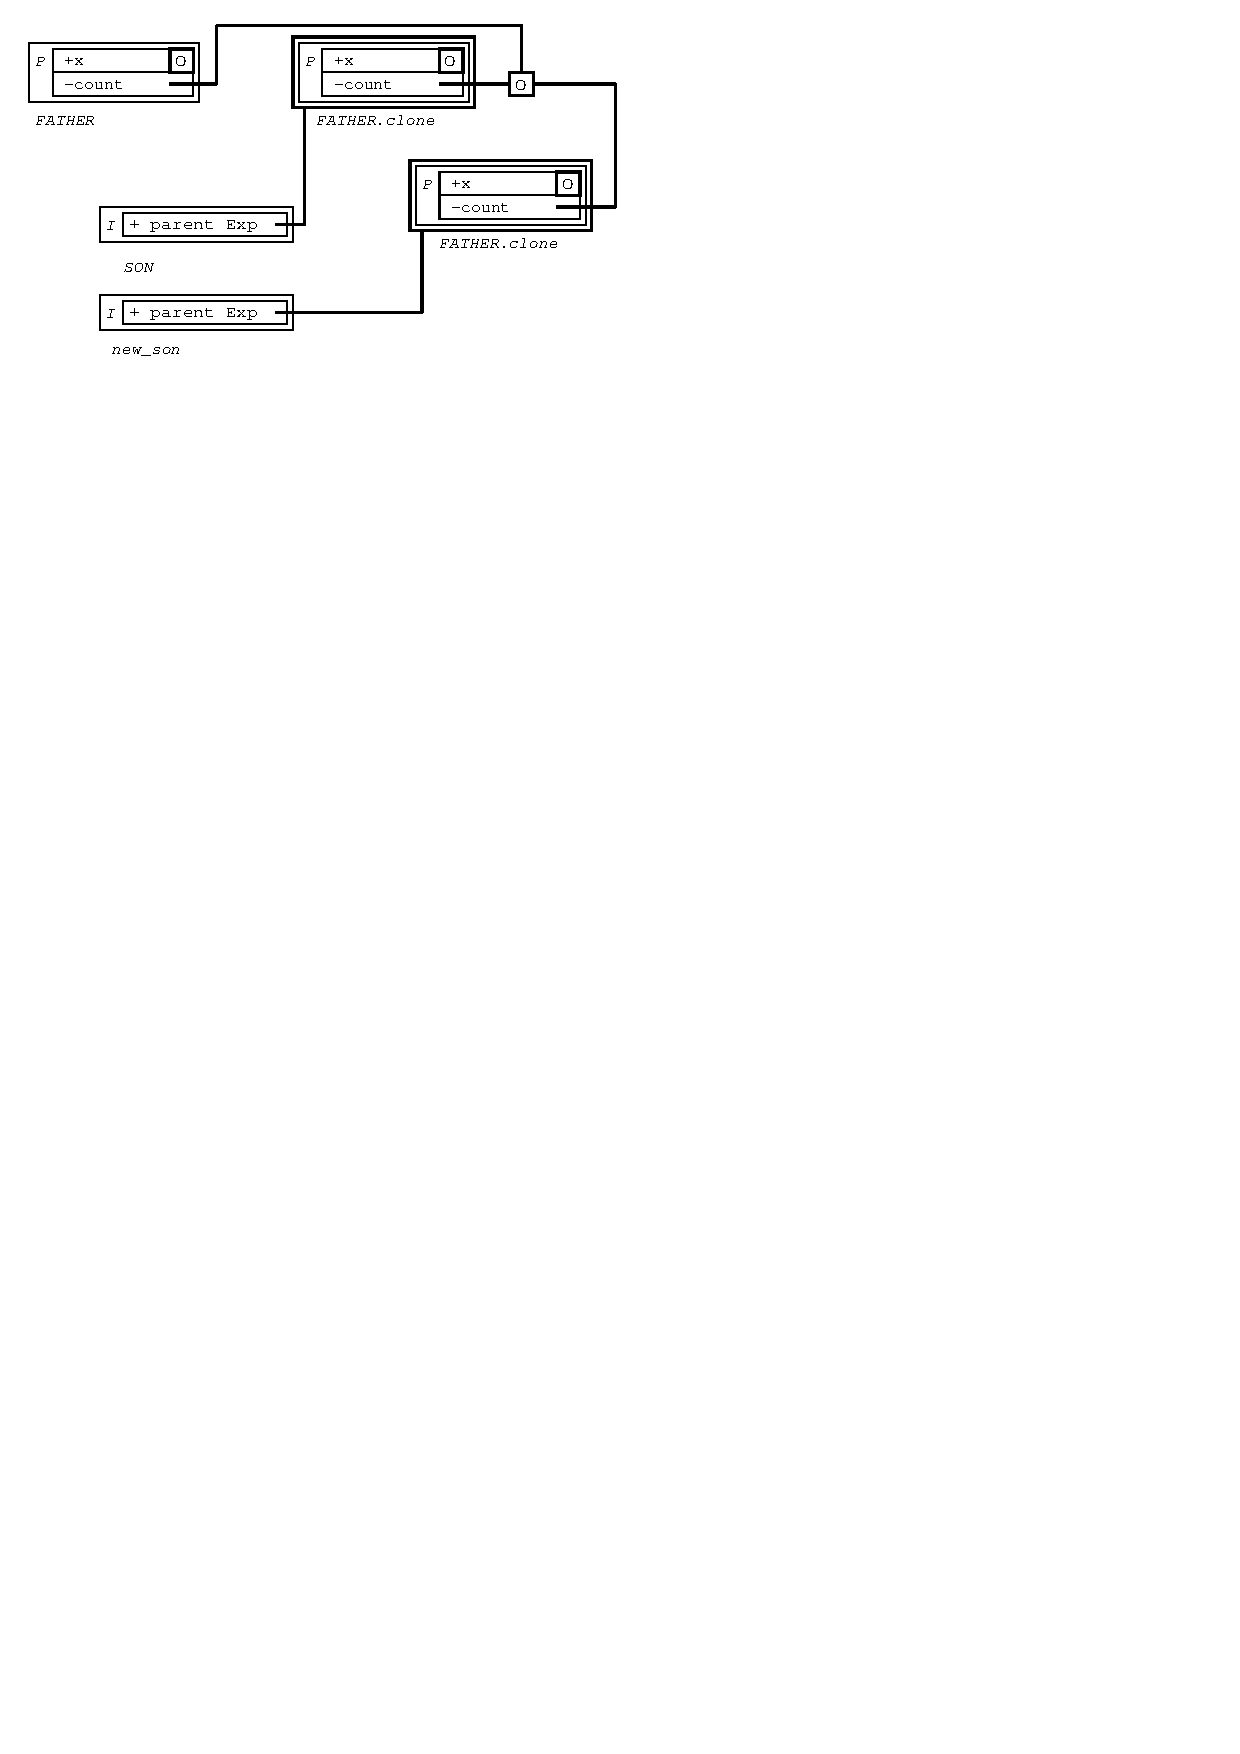
\includegraphics[scale=1.0]{figures/inherit_expanded_1} 
\end{center}

\begin{alltt}
  new\_son.{\bf{}inc\_x};
  new\_son.{\bf{}inc\_count};
\end{alltt}
\begin{center}
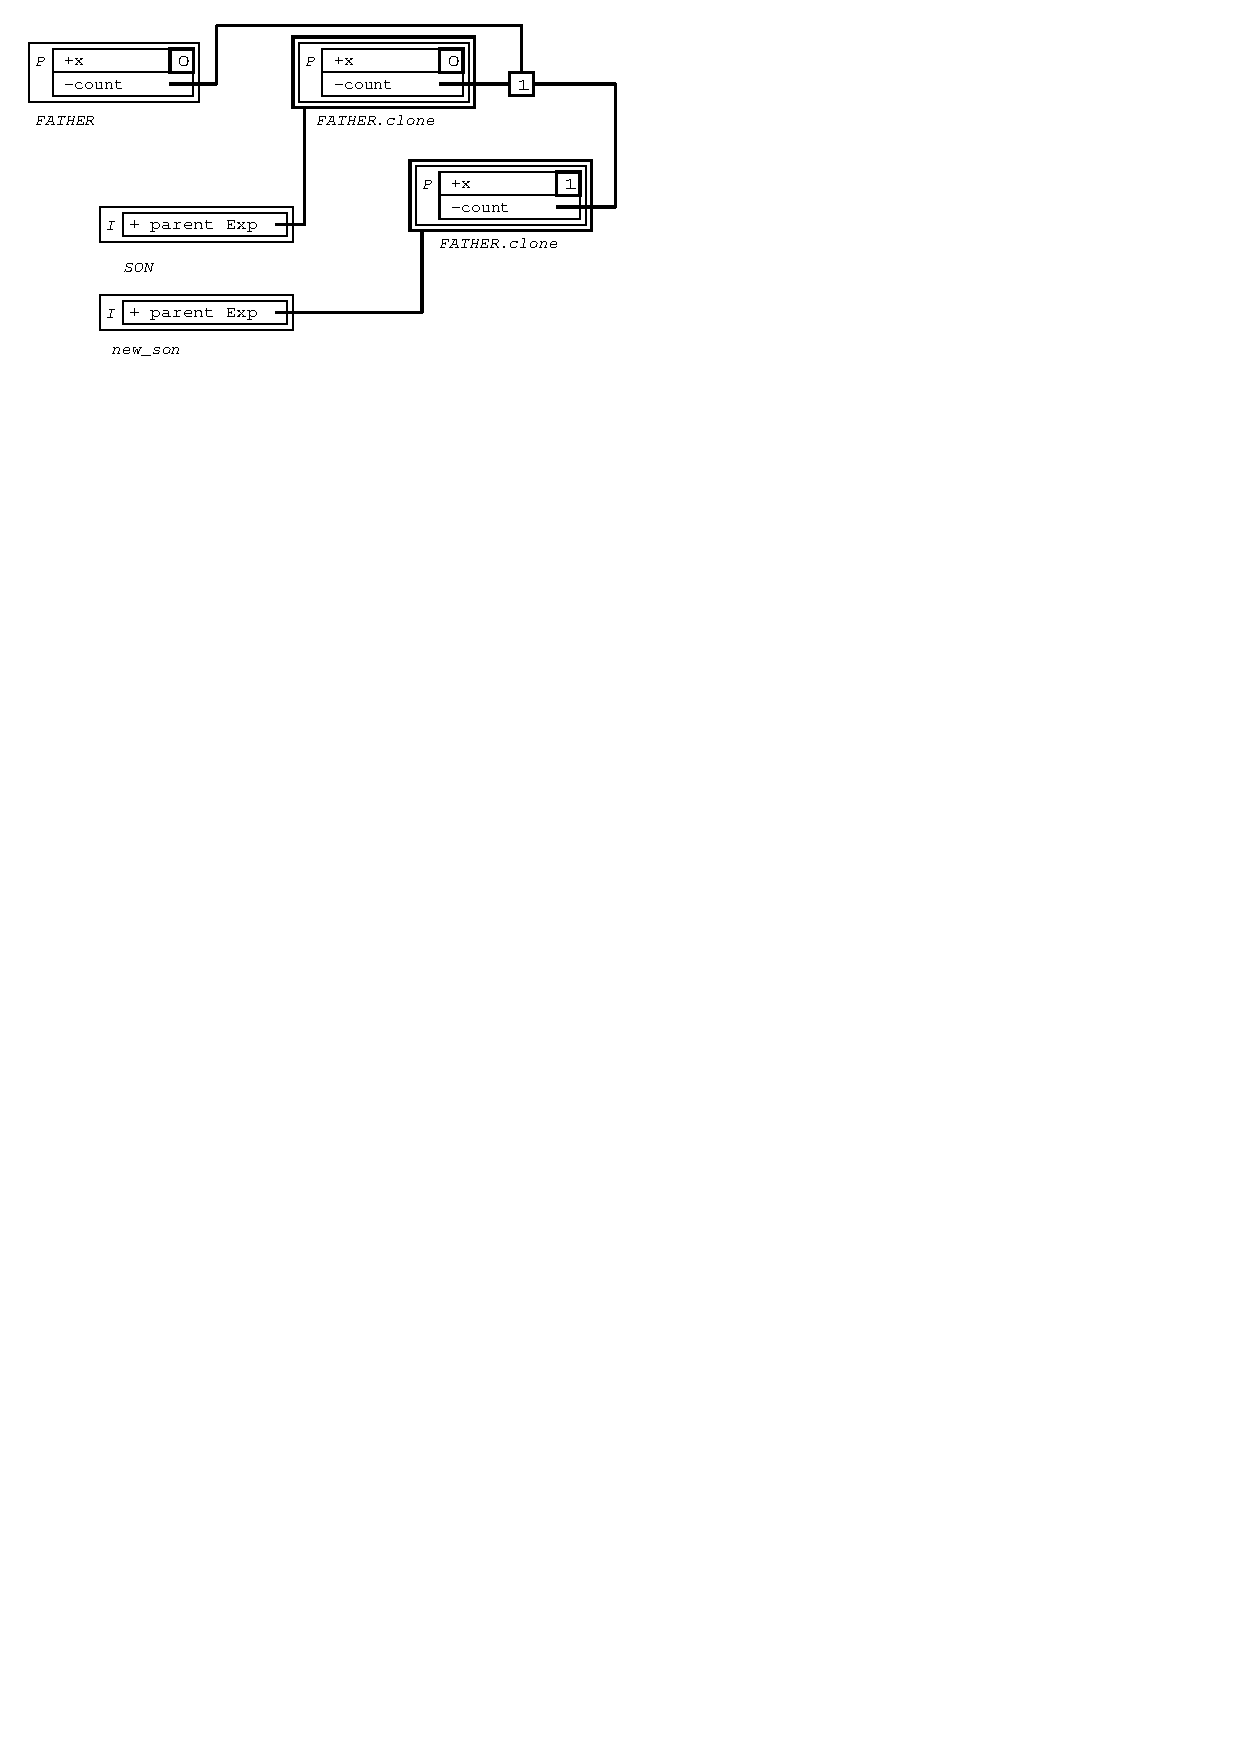
\includegraphics[scale=1.0]{figures/inherit_expanded_2} 
\end{center}

\begin{alltt}
  new\_son.{\bf{}change\_parent} ({\sc{}father}.{\bf{}clone});
\end{alltt}
\begin{center}
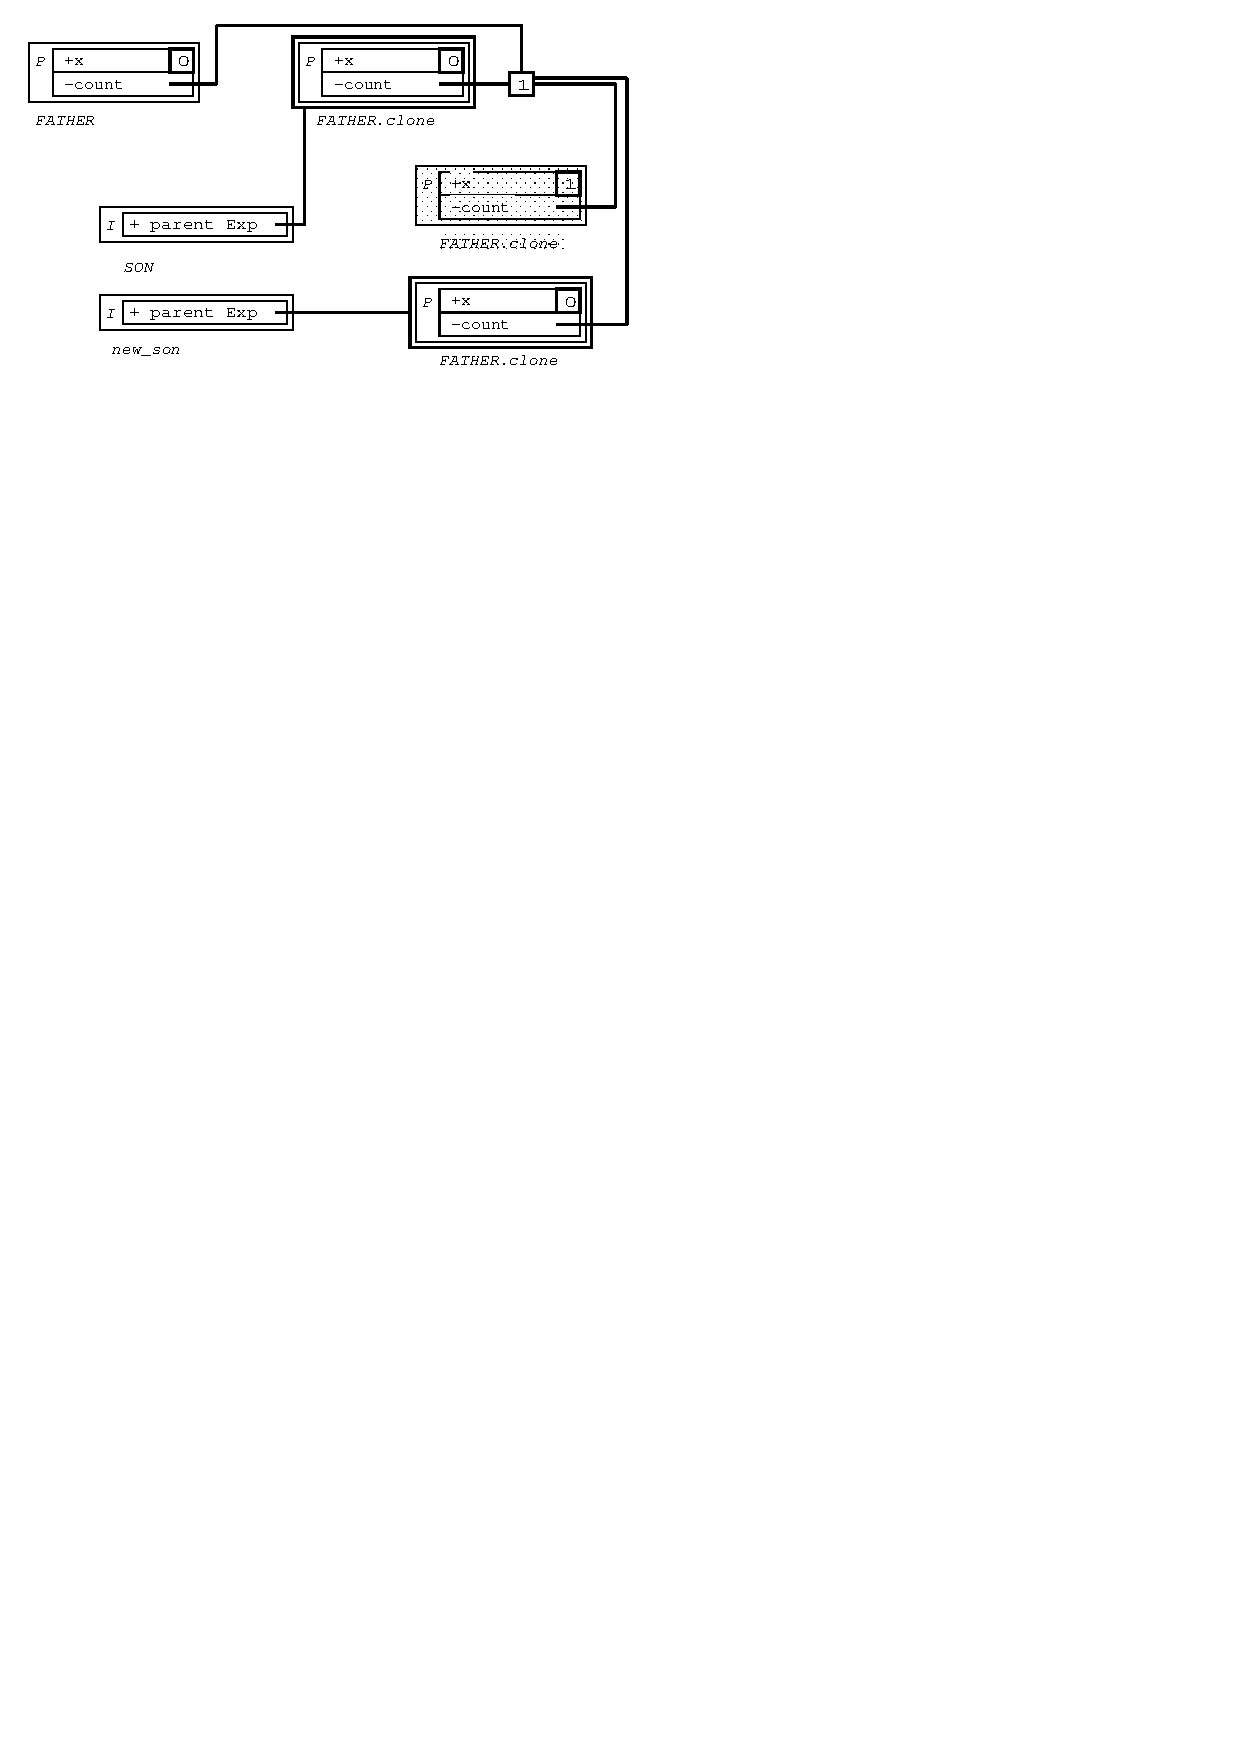
\includegraphics[scale=1.0]{figures/inherit_expanded_3} 
\end{center}

\begin{alltt}
  new\_son.{\bf{}inc\_x};
  new\_son.{\bf{}inc\_count};
\end{alltt}
\begin{center}
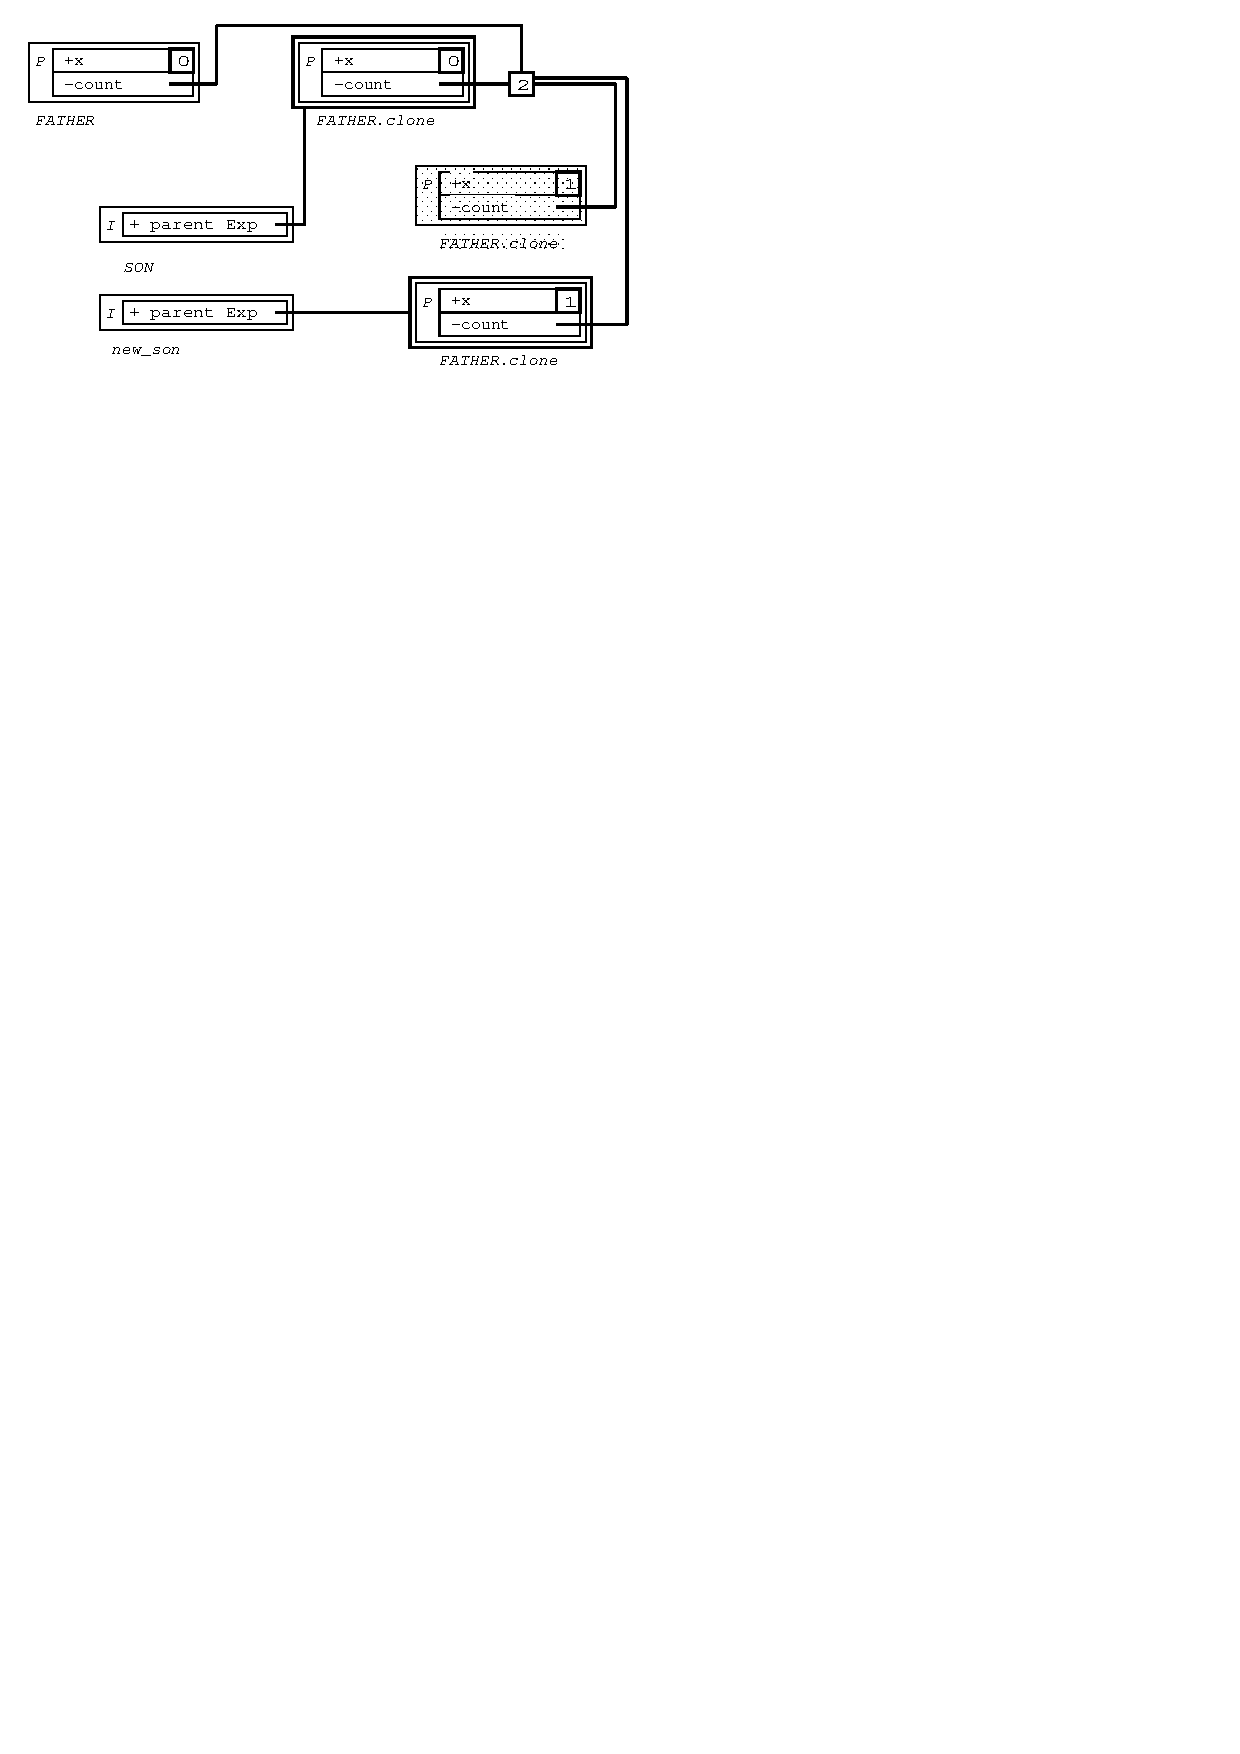
\includegraphics[scale=1.0]{figures/inherit_expanded_4} 
\end{center}

Note: This kind of inheritance is similar to inheritance in object oriented languages based on class.\\
~\\
A parent can also be defined with the the {\bf{} -} symbol and the {\bf{}Expanded} keyword. The parents are now shared.
\begin{alltt}
{\bf{}Section Inherit}
  - {\bf{} parent}:{\bf{}Expanded} {\sc{}father};
\end{alltt}
The value of the parent is already initialised.
\begin{center}
Object {\sc{}father}
\end{center}
\begin{alltt} 
{\bf{}Section Header}
  + {\bf{}name}     := {\sc{}father};          

{\bf{}Section Public}
  + {\bf{}x}    :{\sc{}integer};
  - {\bf{}inc\_x} <- ( x := x + 1; );
  - {\bf{}count}:{\sc{}integer};
  - {\bf{}inc\_count} <- ( count := count + 1; );
\end{alltt}
\begin{center}
Object {\sc{}son}
\end{center}
\begin{alltt} 
{\bf{}Section Header}
  + {\bf{}name}     := {\sc{}son};          

{\bf{}Section Inherit}
  - {\bf{}parent}:{\bf{}Expanded} {\sc{}father};
{\bf{}Section Public}
  - {\bf{}change\_parent} p:{\sc{}father} <- ( parent := p; );
\end{alltt}
\begin{center}
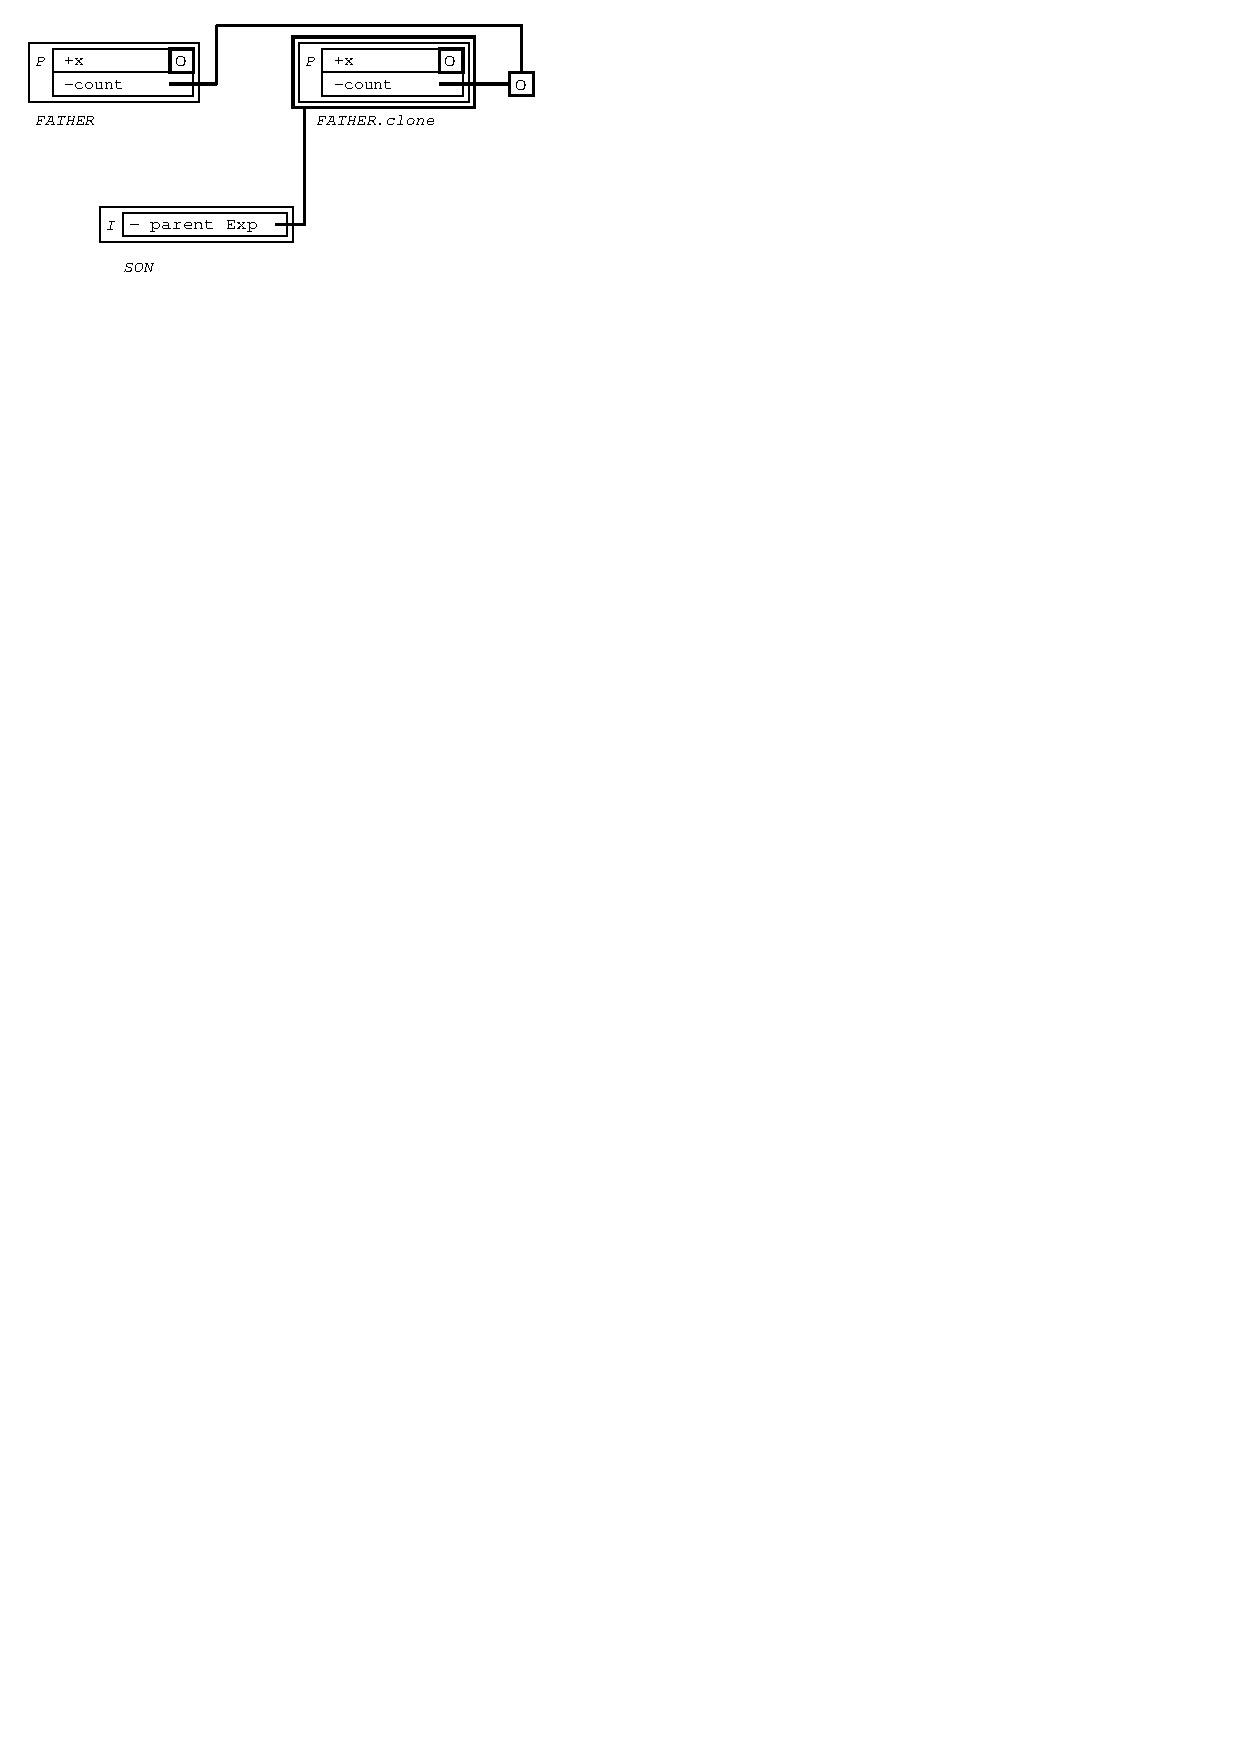
\includegraphics[scale=1.0]{figures/inherit_expanded_minus_0}
\end{center}

\begin{alltt}
  new\_son := {\sc{}son}.{\bf{}clone};
\end{alltt}
\begin{center}
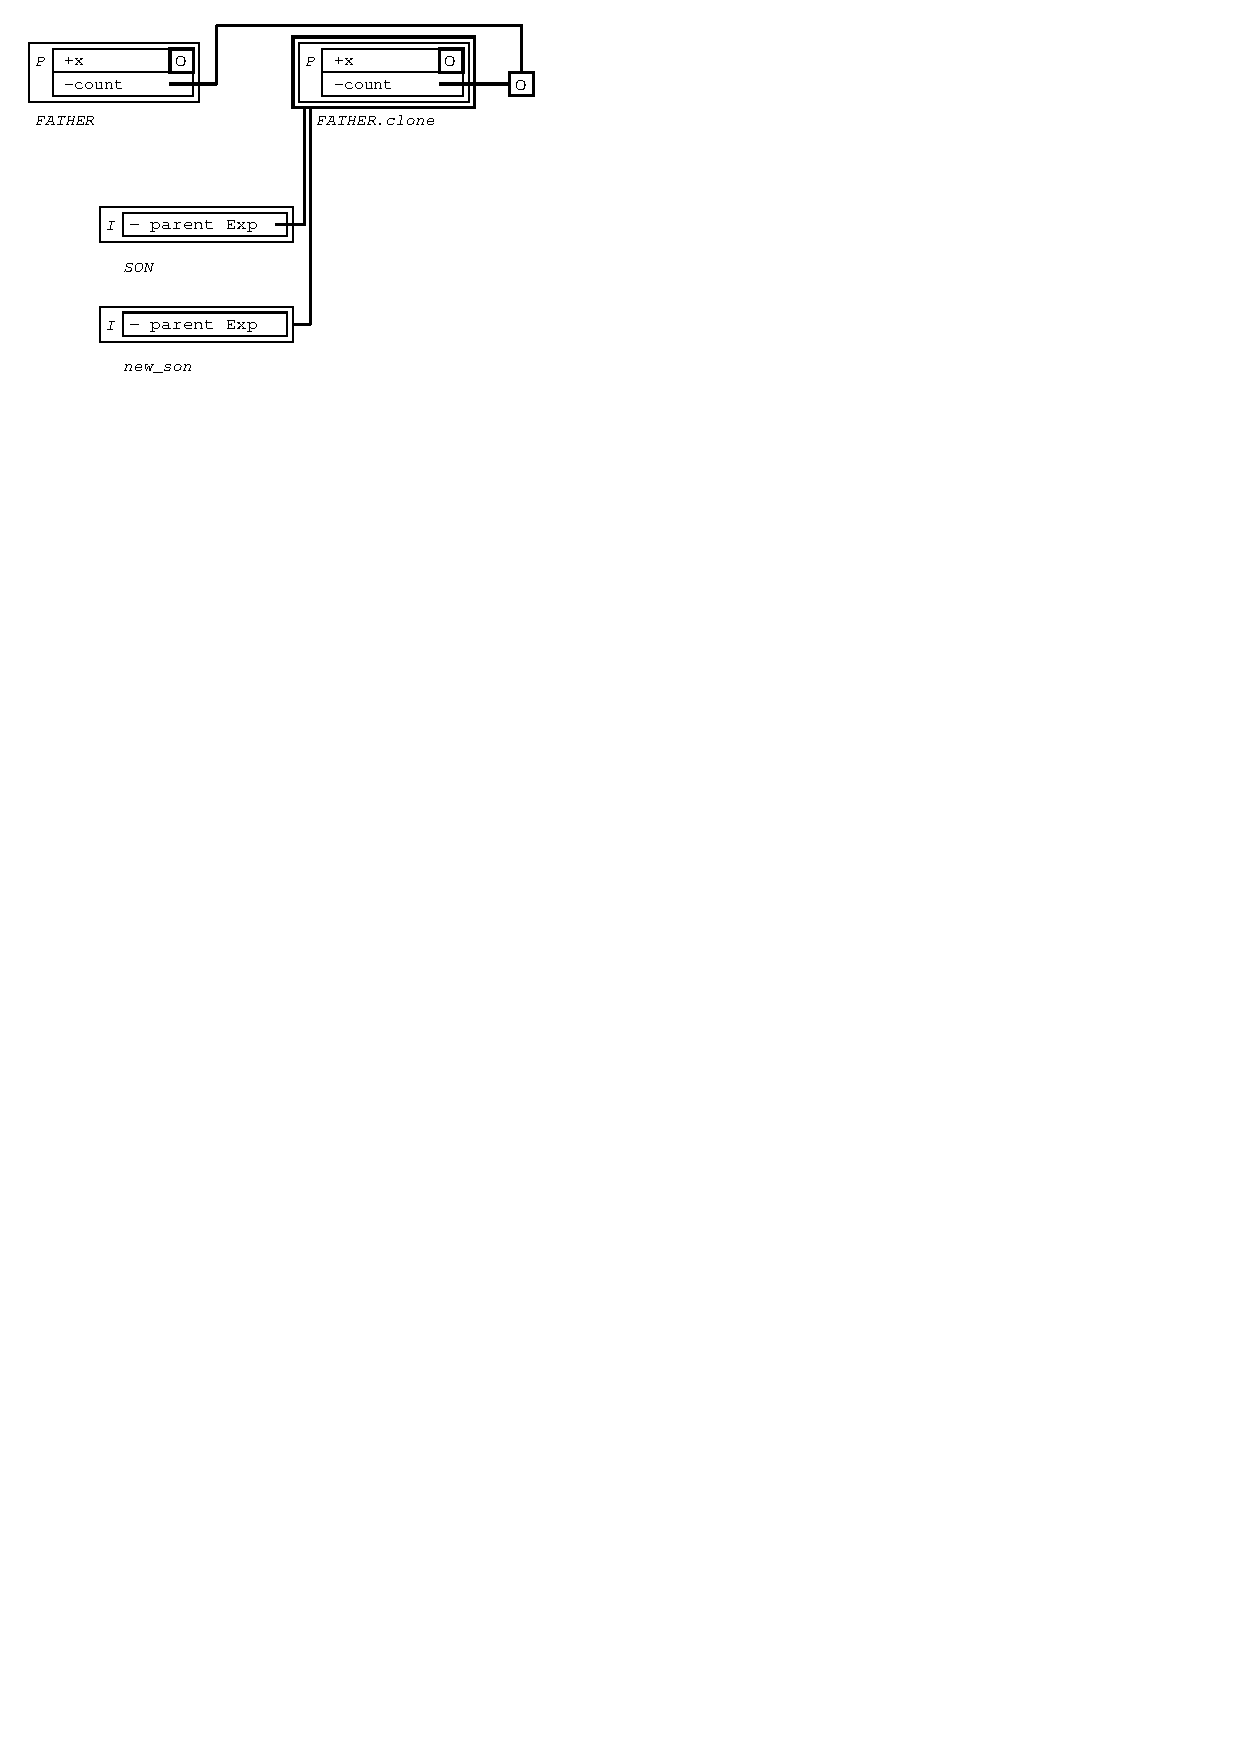
\includegraphics[scale=1.0]{figures/inherit_expanded_minus_1} 
\end{center}

\begin{alltt}
  new\_son.{\bf{}inc\_x};
  new\_son.{\bf{}inc\_count};
\end{alltt}
\begin{center}
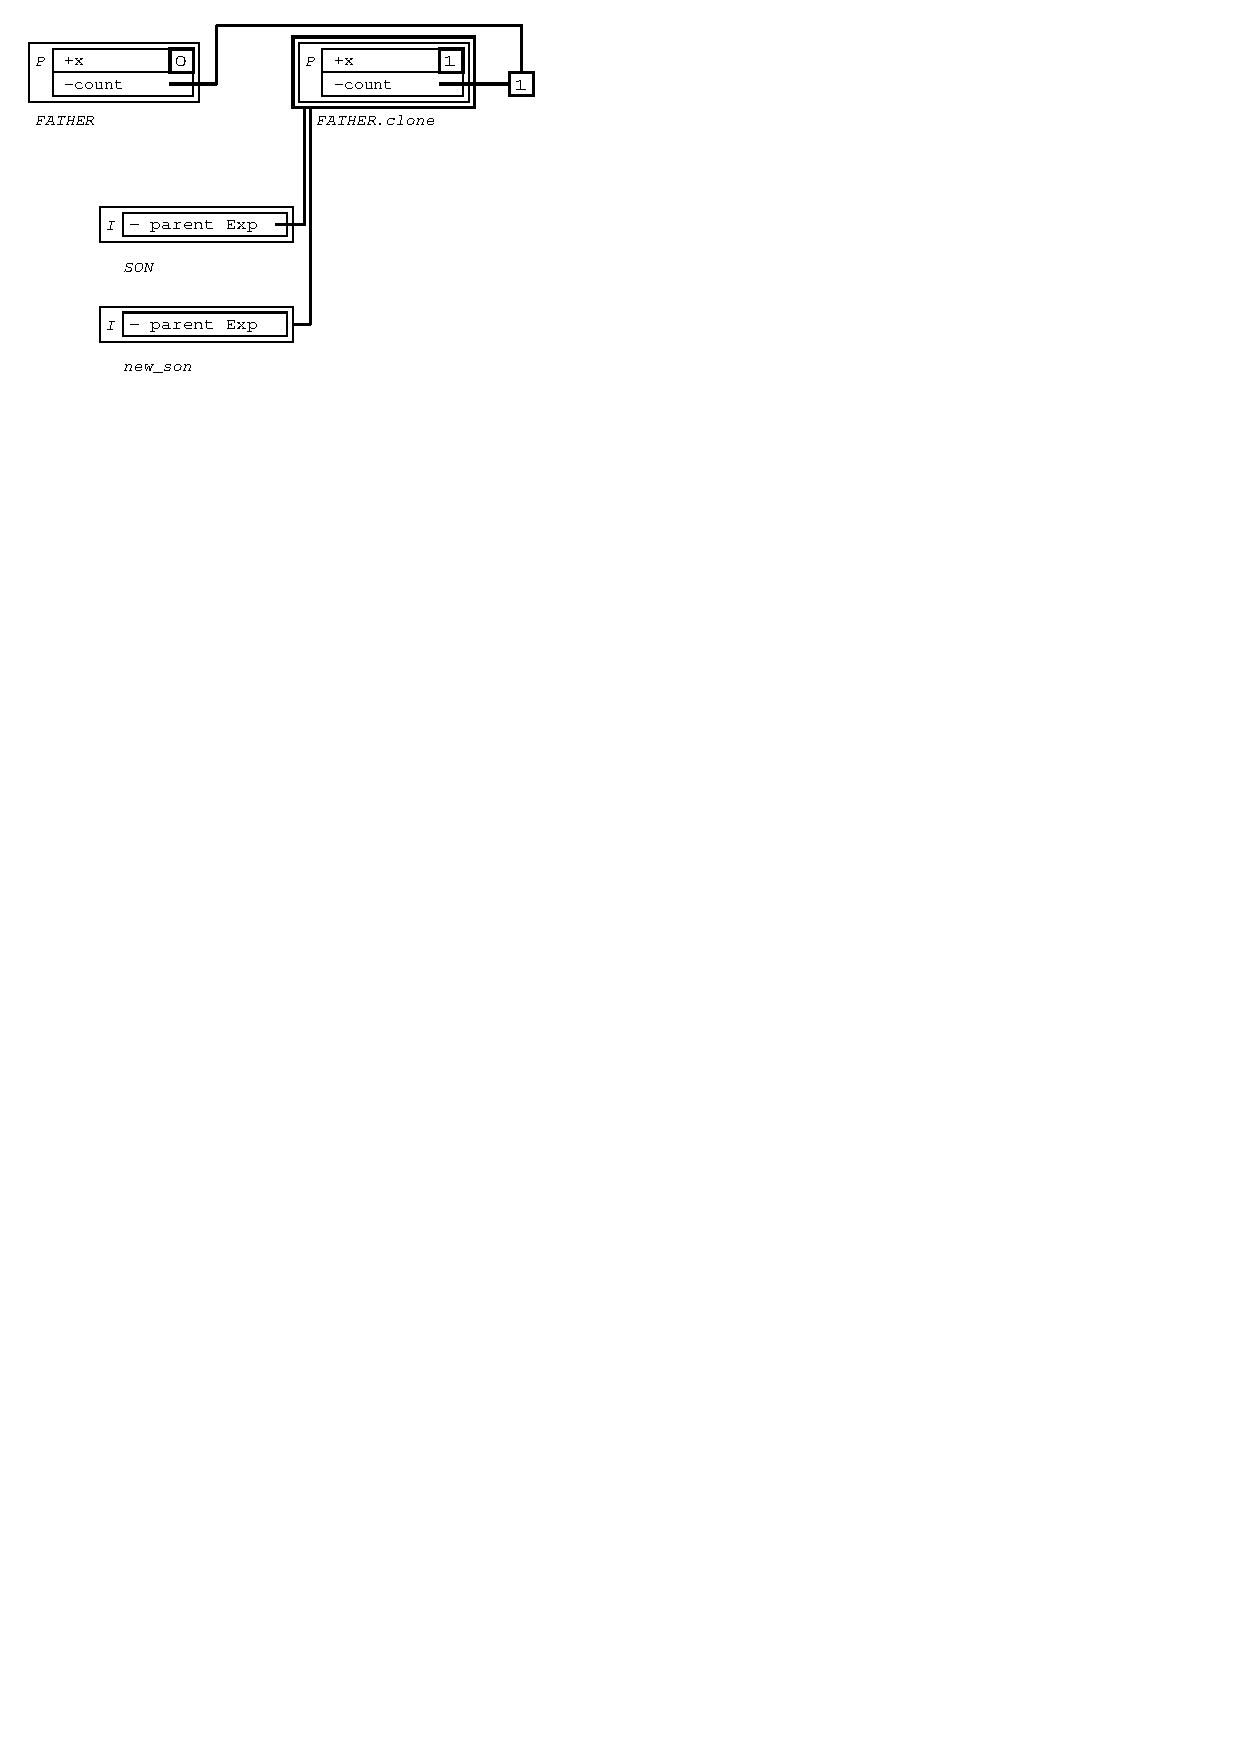
\includegraphics[scale=1.0]{figures/inherit_expanded_minus_2} 
\end{center}

\begin{alltt}
  new\_son.{\bf{}change\_parent} ({\sc{}father}.{\bf{}clone});
\end{alltt}
\begin{center}
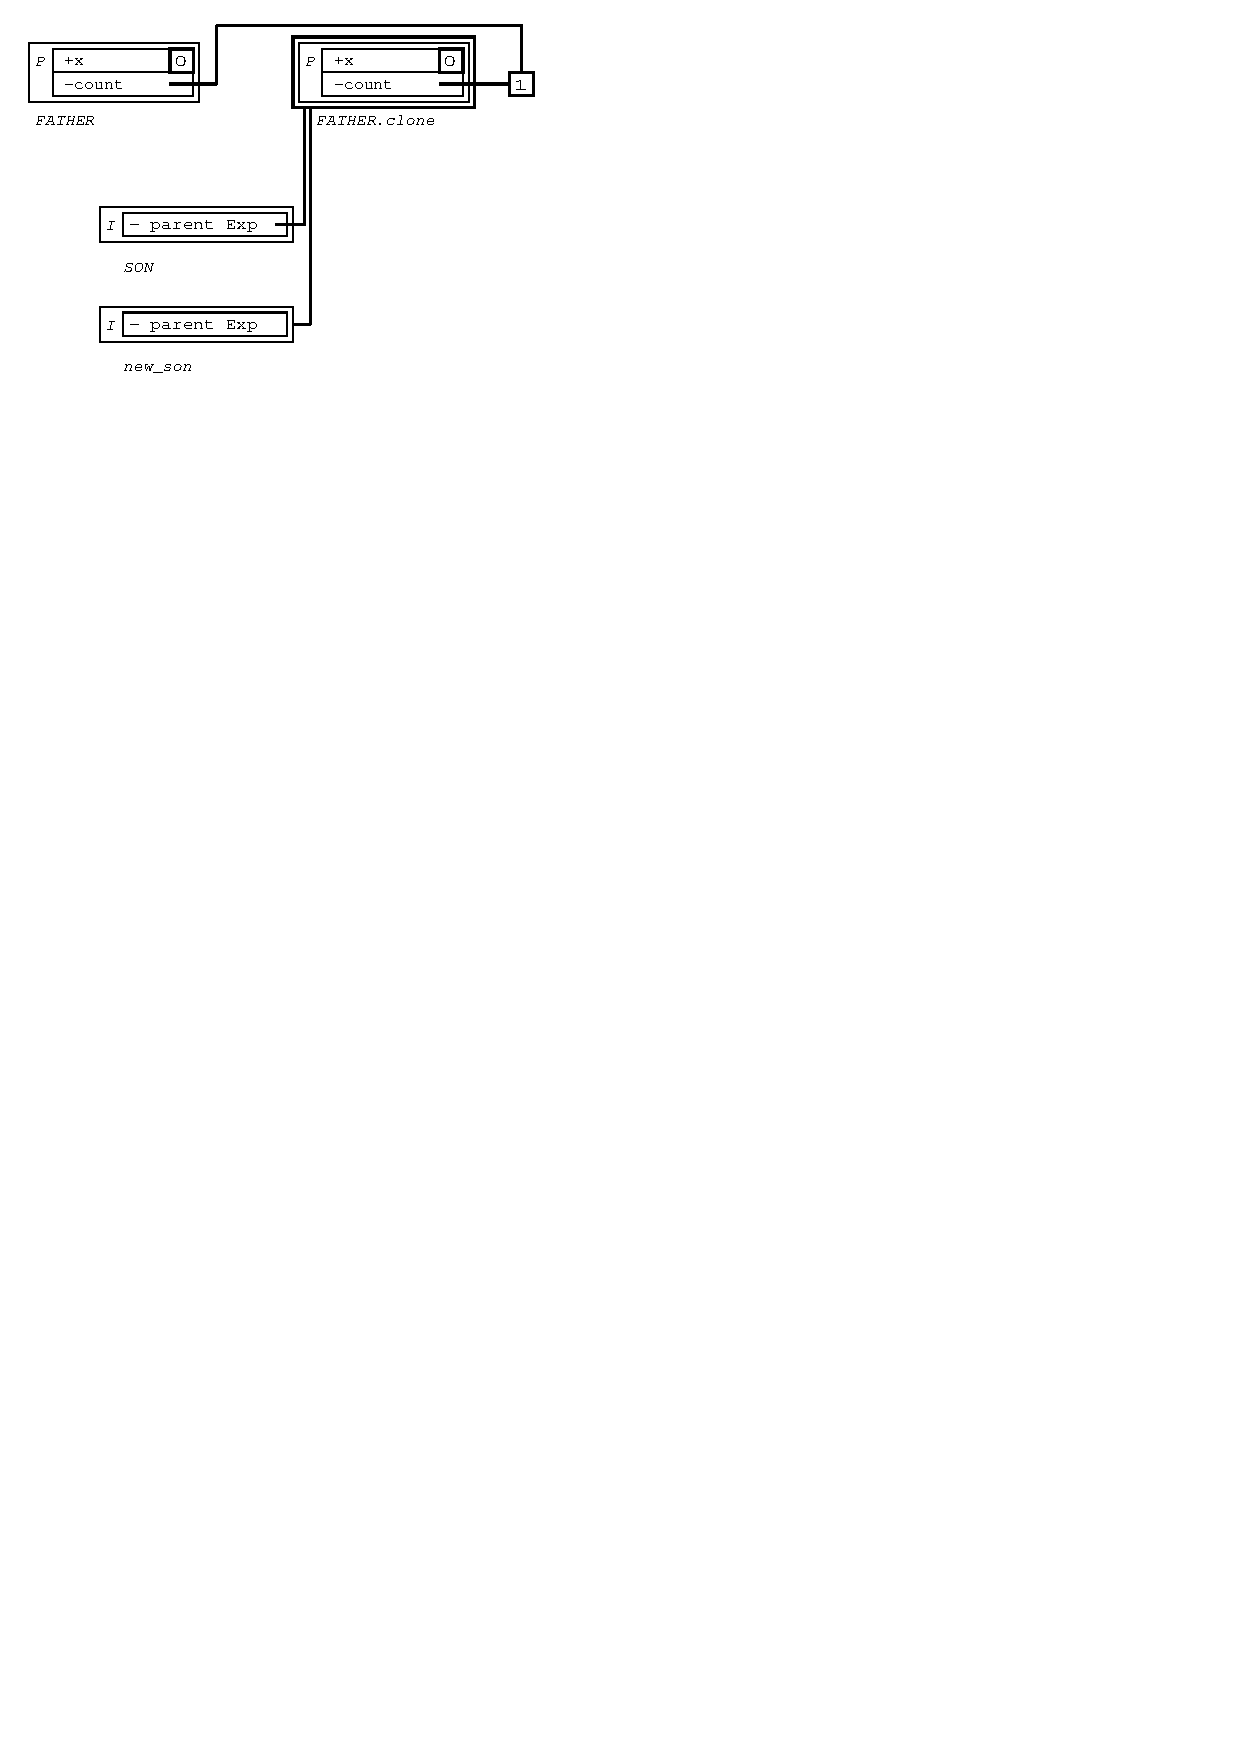
\includegraphics[scale=1.0]{figures/inherit_expanded_minus_3} 
\end{center}

\begin{alltt}
  new\_son.{\bf{}inc\_x};
  new\_son.{\bf{}inc\_count};
\end{alltt}
\begin{center}
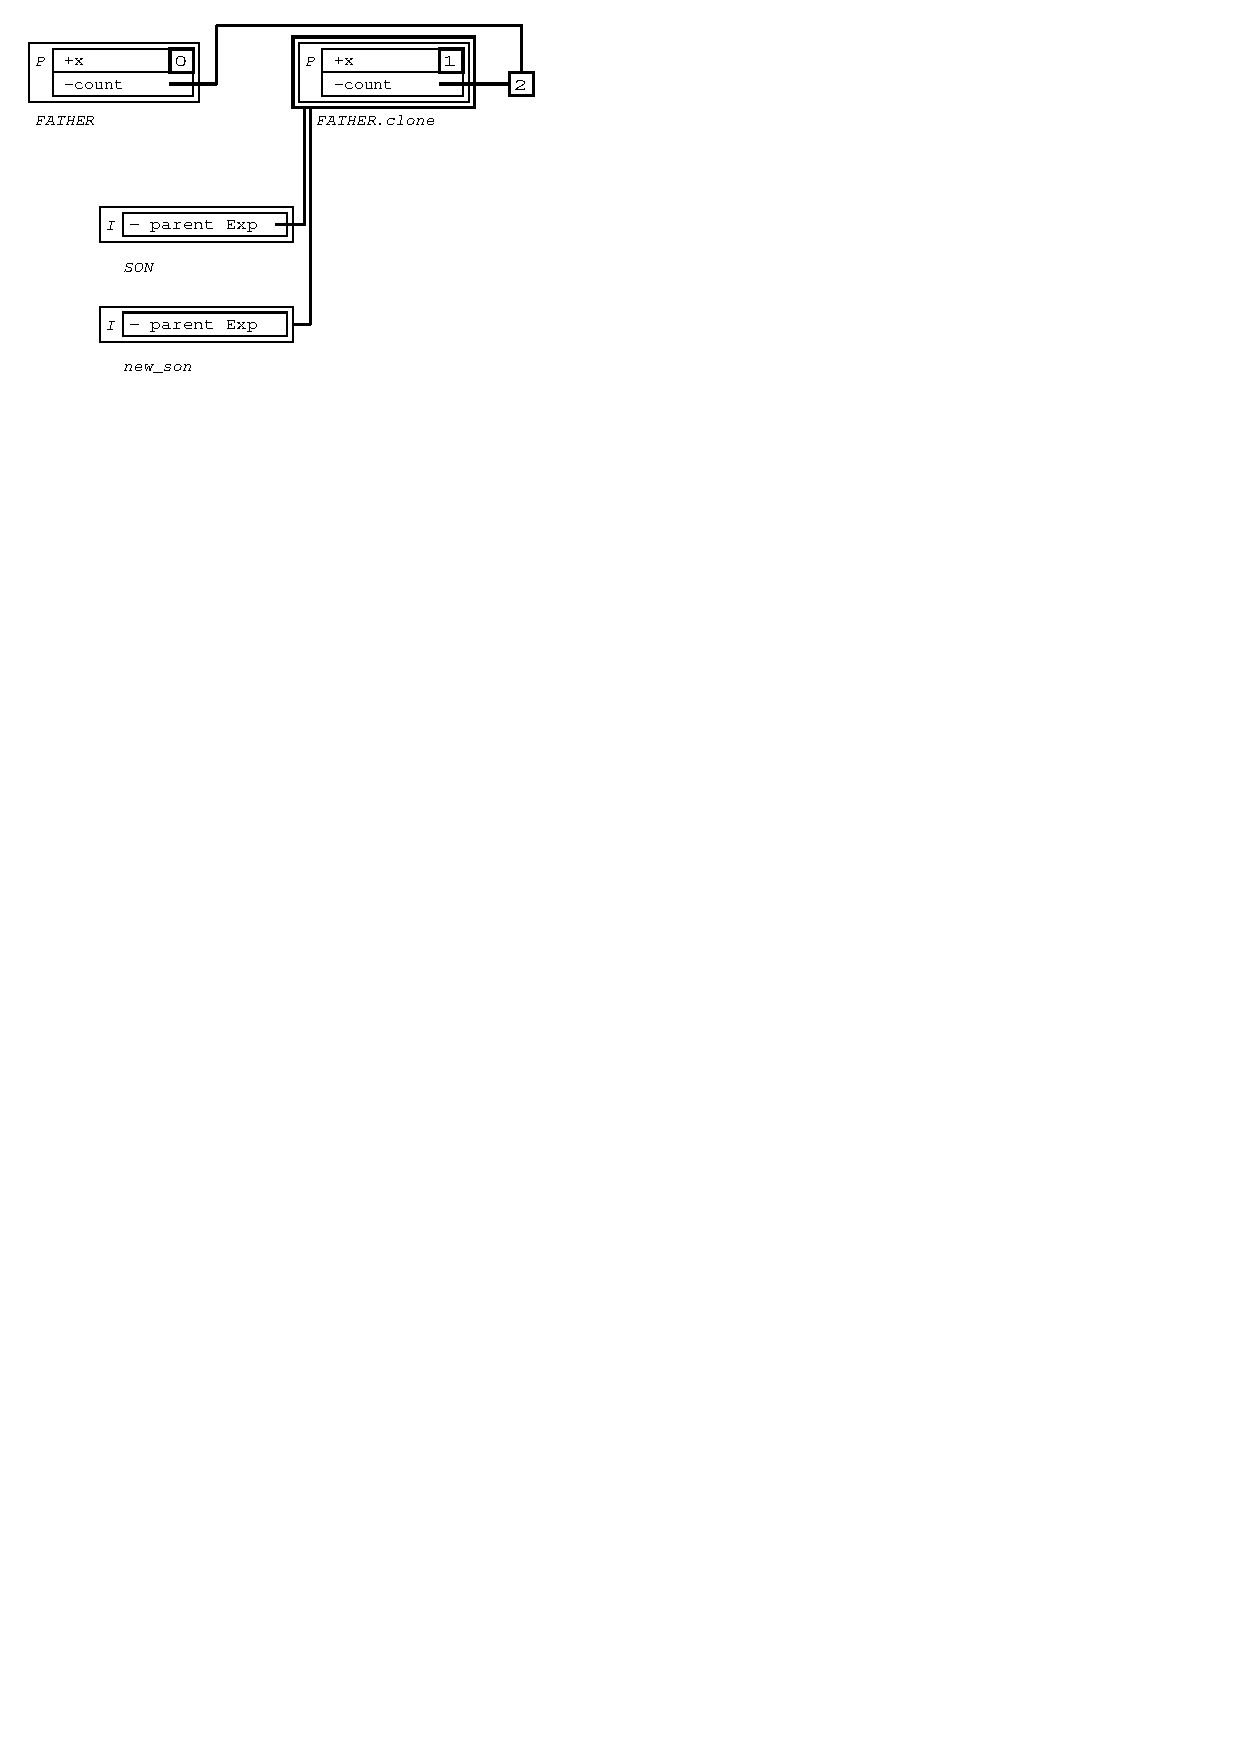
\includegraphics[scale=1.0]{figures/inherit_expanded_minus_4} 
\end{center}
%.........................................................
\subsubsection{Immediate/delayed evaluation}
\label{language_reference:section_identifiers:inherit_section:parent_evaluation}
%.........................................................
%
\index{Inheritance, evaluation of parents}
\warning{} The evaluation of the heritage slots depends on their
order of declaration

\begin{itemize}
\item[$\bullet$]{Evaluation after the loading of the
prototype:
\begin{alltt} 
{\bf{}Section Inherit}
  + {\bf{}parent}:{\sc{}expr} := {\sc{}expr};
\end{alltt}}

\item[$\bullet$]{Evaluation every time the lookup algorithm reaches 
this slot (this should be avoided, because it is obviously very expensive):
\begin{alltt} 
{\bf{}Section Inherit}
  - {\bf{}parent}:{\sc{}object} <- {\bf{}search\_parent};
\end{alltt}
Here, {\it{}search\_parent} is a method to evaluate the parent.\\

{\it{}Other example}:
\begin{alltt} 
{\bf{}Section Inherit}
  - {\bf{}parent}:{\sc{}object} <-
  ( + result:{\sc{}object};
    ({\bf{}flag\_depend}).{\bf{}if} \{
      result := {\sc{}value};
    \} {\bf{}else} \{
      result := {\sc{}affect};
    \};
    result
  );
\end{alltt}
\warning{} the {\bf{}flag\_depend} slot must be present in the lower of the inheritance tree.
}\end{itemize}
%.........................................................
\subsubsection{Static type and visibility of the slots}
\label{language_reference:section_identifiers:inherit_section:visibility_slots}
%.........................................................
%
\index{Slot, visibility}
~\\
The static type of a slot parent must correspond to the 
first common ancestor of the parents possible dynamics.
\\
About the visibility of the slots, the static tree of 
heritage shows the slots accessible.
\begin{alltt} 
{\bf{}Section Header}
  + {\bf{}name} := {\sc{}a};

{\bf{}Section Public}
  + {\bf{}bar} <- /* \ldots */
  + {\bf{}foo} <- /* \ldots */\\

{\bf{}Section Header}
  + {\bf{}name} := {\sc{}b};

{\bf{}Section Inherit}
  + {\bf{}parent}:{\sc{}a} := {\sc{}a};
{\bf{}Section Public}
  + {\bf{}bar} <- /* \ldots */
  + {\bf{}toto} <- /* \ldots */\\

{\bf{}Section Header}
  + {\bf{}name} := {\sc{}c};

{\bf{}Section Inherit}
  + {\bf{}parent}:{\sc{}a} := {\sc{}a};
{\bf{}Section Public}
  + {\bf{}titi} <- /* \ldots */
  + {\bf{}foo} <- /* \ldots */\\

{\bf{}Section Header}
  + {\bf{}name} := {\sc{}d};

{\bf{}Section Inherit}
  + {\bf{}parent}:{\sc{}a} <-
  (
  ...            // code that can be dynamically {\sc{}b} or {\sc{}c}
  );
{\bf{}Section Public}
  + {\bf{}new} <- /* \ldots */
  + {\bf{}toto} <- /* \ldots */
\end{alltt}
%===========================================================
\begin{center}
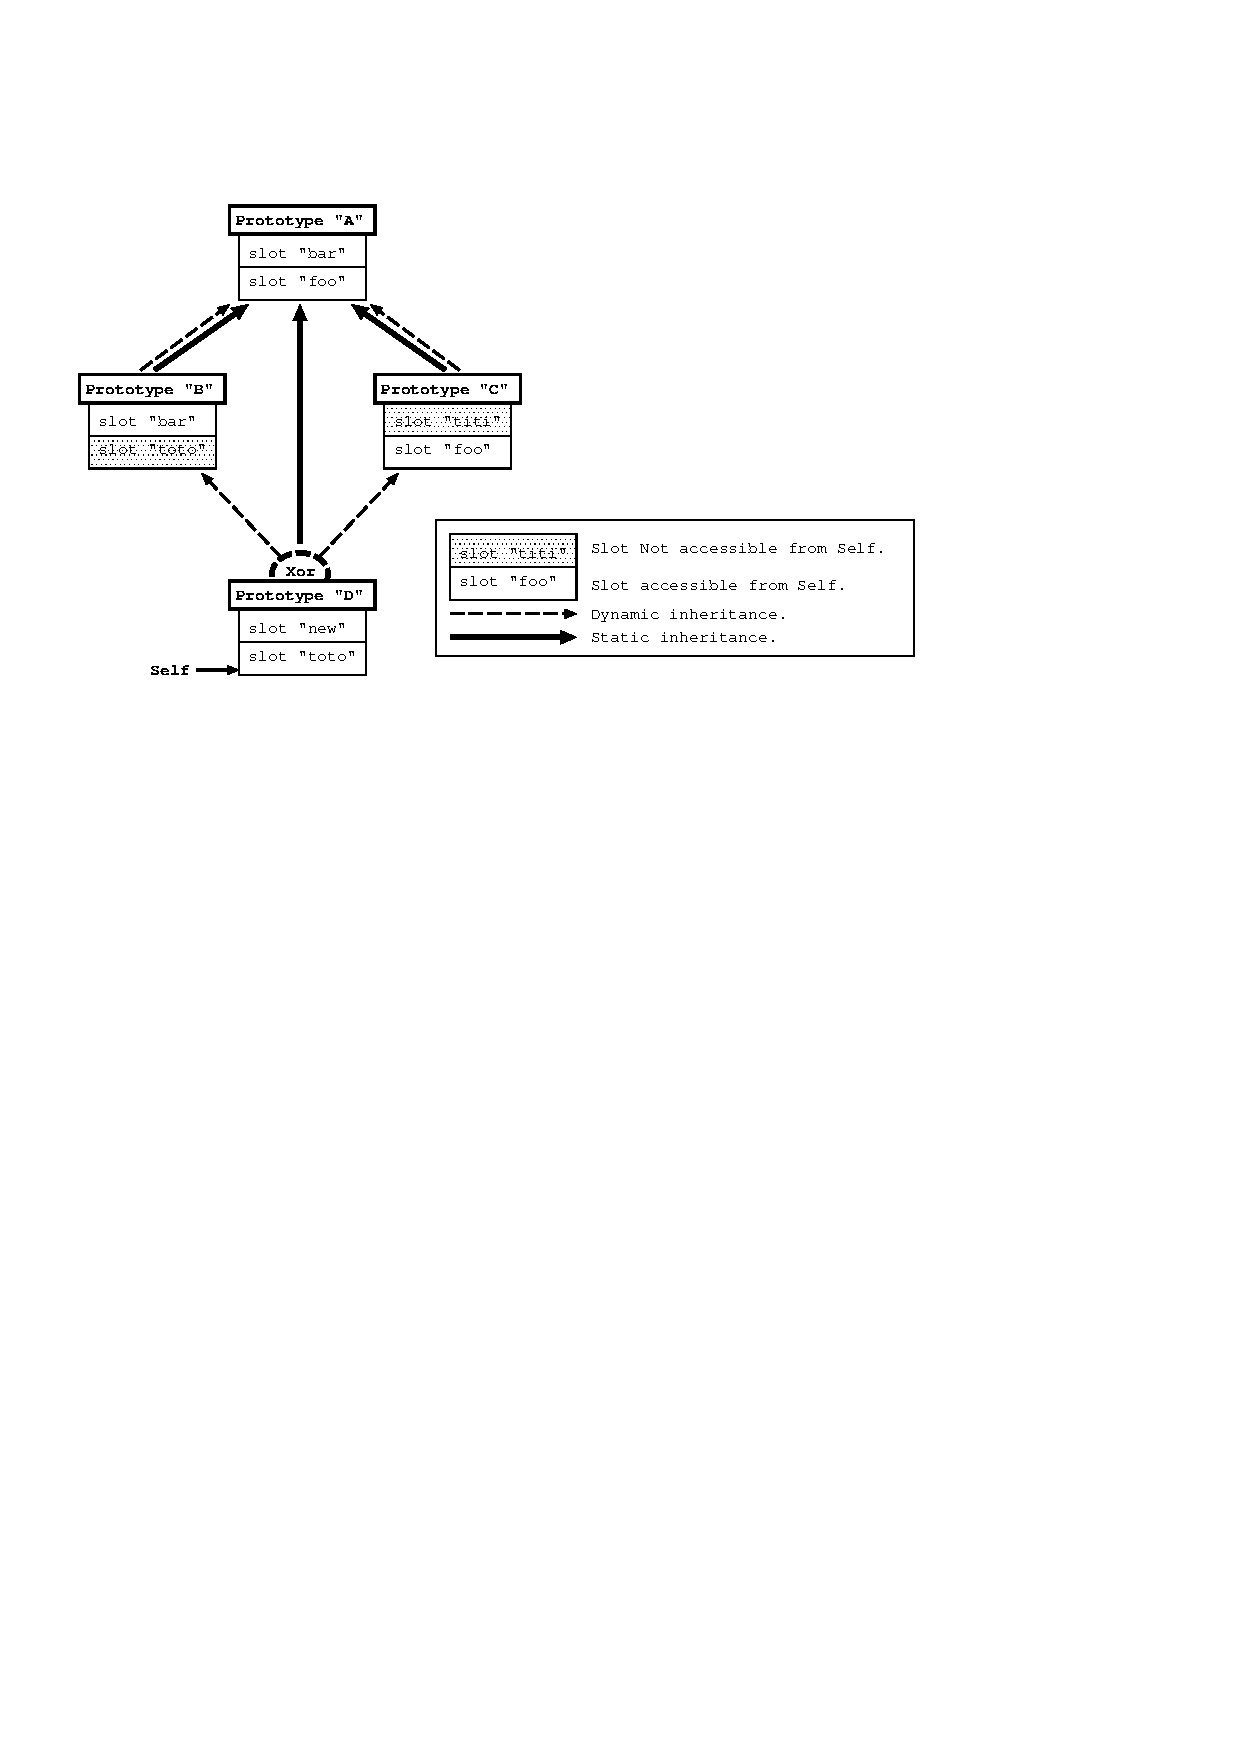
\includegraphics[scale=1.0]{figures/type_parent}
\end{center}
%===========================================================
\begin{alltt}
{\bf{}Section Header}
  + {\bf{}name} := {\sc{}test};

{\bf{}Section Public}
  - {\bf{}main} :=
  ( + object_d:{\sc{}d};
    object_d := {\sc{}d}.clone;
    object_d.{\bf{}bar};   // Ok, from {\sc{}a} or from {\sc{}b} (dynamic inheritance)
    object_d.{\bf{}foo};   // Ok, from {\sc{}a} or from {\sc{}c} (dynamic inheritance)
    object_d.{\bf{}new};   // Ok, from {\sc{}d}
    object_d.{\bf{}toto};  // Ok, from {\sc{}d} (redefinition in {\sc{}d})
    object_d.{\bf{}titi};  // Error: slot not accessible     
  );
\end{alltt}

%---------------------------------------------------------
\subsubsection{The lookup algorithm}
\label{language_reference:section_identifiers:inherit_section:lookup}
%---------------------------------------------------------
%
\index{Lookup algorithm}

The lookup algorithm is the name of the algorithm used to resolve
message send (or dynamic dispatch).
It determines which precise method is called.

Let $M$ be the complete name of the called method, with commas or
keywords, if any (see slot names in
section \ref{language_reference:slot_descriptors} page
\pageref{language_reference:slot_descriptors}).
Let $R$ be the receiver of the message send; in case the receiver is
implicit, $R$ is {\tt self}.
Let $T$ be the dynamic type of $R$.

The lookup algorithm works as follows: 
\begin{enumerate}
\item{Look for method $M$ in the current prototype $T$, searching
      code slots.\\
      Since there is no overloading in Lisaac, there should be at
      most one slot matching $M$.\\
      If one was found, the lookup algorithm stops, the target method
      has been found and the message send can proceed.\\
      If none was found, continue with step 2.
}
\item{Recursively look for method $M$ in all the parents of the current
      prototype $T$, until one is found or all parents have been
      examined.\\
      If the matching method has been found, the lookup algorithm
      stops, the target method has been found and the message send can
      proceed.\\  
      If none was found, which indicates an error from the developper,
      an error message is emitted.
}
\end{enumerate}

Note that at step 1,  since there is no overloading in Lisaac, there
should be at most one slot matching $M$.
The order of declaration of code slots in $T$ is thus irrelevant.

Conversely, the order of declaration of parent slots is highly 
relevant. 
Indeed, during step 2, parent slots are searched recursively, that is in
depth-first manner.  
They are also examined in the order of declaration in the source code
(top to bottom).
As a consequence, in case of multiple inheritance, if $n$ parent slots
($ 2 \le n$) refer to prototypes that contain the searched method $M$,
it is the $M$ contained in the first of those $n$ parent slots that
shall be called.
Thus multiple inheritance conflicts in Lisaac are solved in a
(depth-first) ``first arrived, first served'' manner.

\begin{alltt}
  {\bf{}- lookup} msg:{\sc{}string} {\bf{}set\_visited} v:{\sc{}set}[{\sc{}object}] :{\sc{}block} <-
    ( + result:{\sc{}block};
      + i:{\sc{}integer};
     
      (! v.{\bf{}has} self).{\bf{}if} \{   
        {\it{}// cycle detection.}
        v.{\bf{}add} self;

        {\it{}// Search in current object.} 
        i := list.lower;
        \{(i <= list.upper) && \{result = {\sc{}null}\}\}.{\bf{}while\_do} \{
          (list.{\bf{}item} i.name == msg).{\bf{}if} \{   
            {\it{}// message found.}
            Result := list.{\bf{}item} i.value;
          \};
          i := i + 1;
        \};

        (result = {\sc{}null}).{\bf{}if} \{
          {\it{}// Search in parent object.}
          i := parent\_list.lower;
          \{(i <= parent\_list.upper) && \{result = {\sc{}null}\}\}.{\bf{}while\_do} \{
            result := parent\_list.{\bf{}item} i.{\bf{}lookup} msg {\bf{}set\_visited} v;
            i := i + 1;
          \};
        \};

      \};
      result 
    );

\end{alltt}

%---------------------------------------------------------
\subsubsection{Resending messages: The equivalent of {\it{}super} in Smalltalk or {\it{}resend} in Self.}
\label{language_reference:section_identifiers:inherit_section:resending}
%---------------------------------------------------------
%
\index{Message, resend}
A message call applied to some parent slot is the natural mechanism 
to achieve he equivalent of {\it{}super} in
Smalltalk or {\it{}resend} in Self. 
This means that the message is sent to the parent with the current object
context.
You can bypass the lookup algorithm by precising the parent on which you call the slot.
\begin{alltt} 
{\bf{}Section Header}
  + {\bf{}name} := {\sc{}father1};

{\bf{}Section Public}
  - {\bf{}method} <- /* \ldots */

{\bf{}Section Header}
  + {\bf{}name} := {\sc{}father2};

{\bf{}Section Public}
  - {\bf{}method} <- /* \ldots */

{\bf{}Section Header}
  + {\bf{}name} := {\sc{}son}
{\bf{}Section Inherit}
  + {\bf{}parent1} := {\sc{}father1};
  + {\bf{}parent2} := {\sc{}father2};
\end{alltt}
\begin{center}
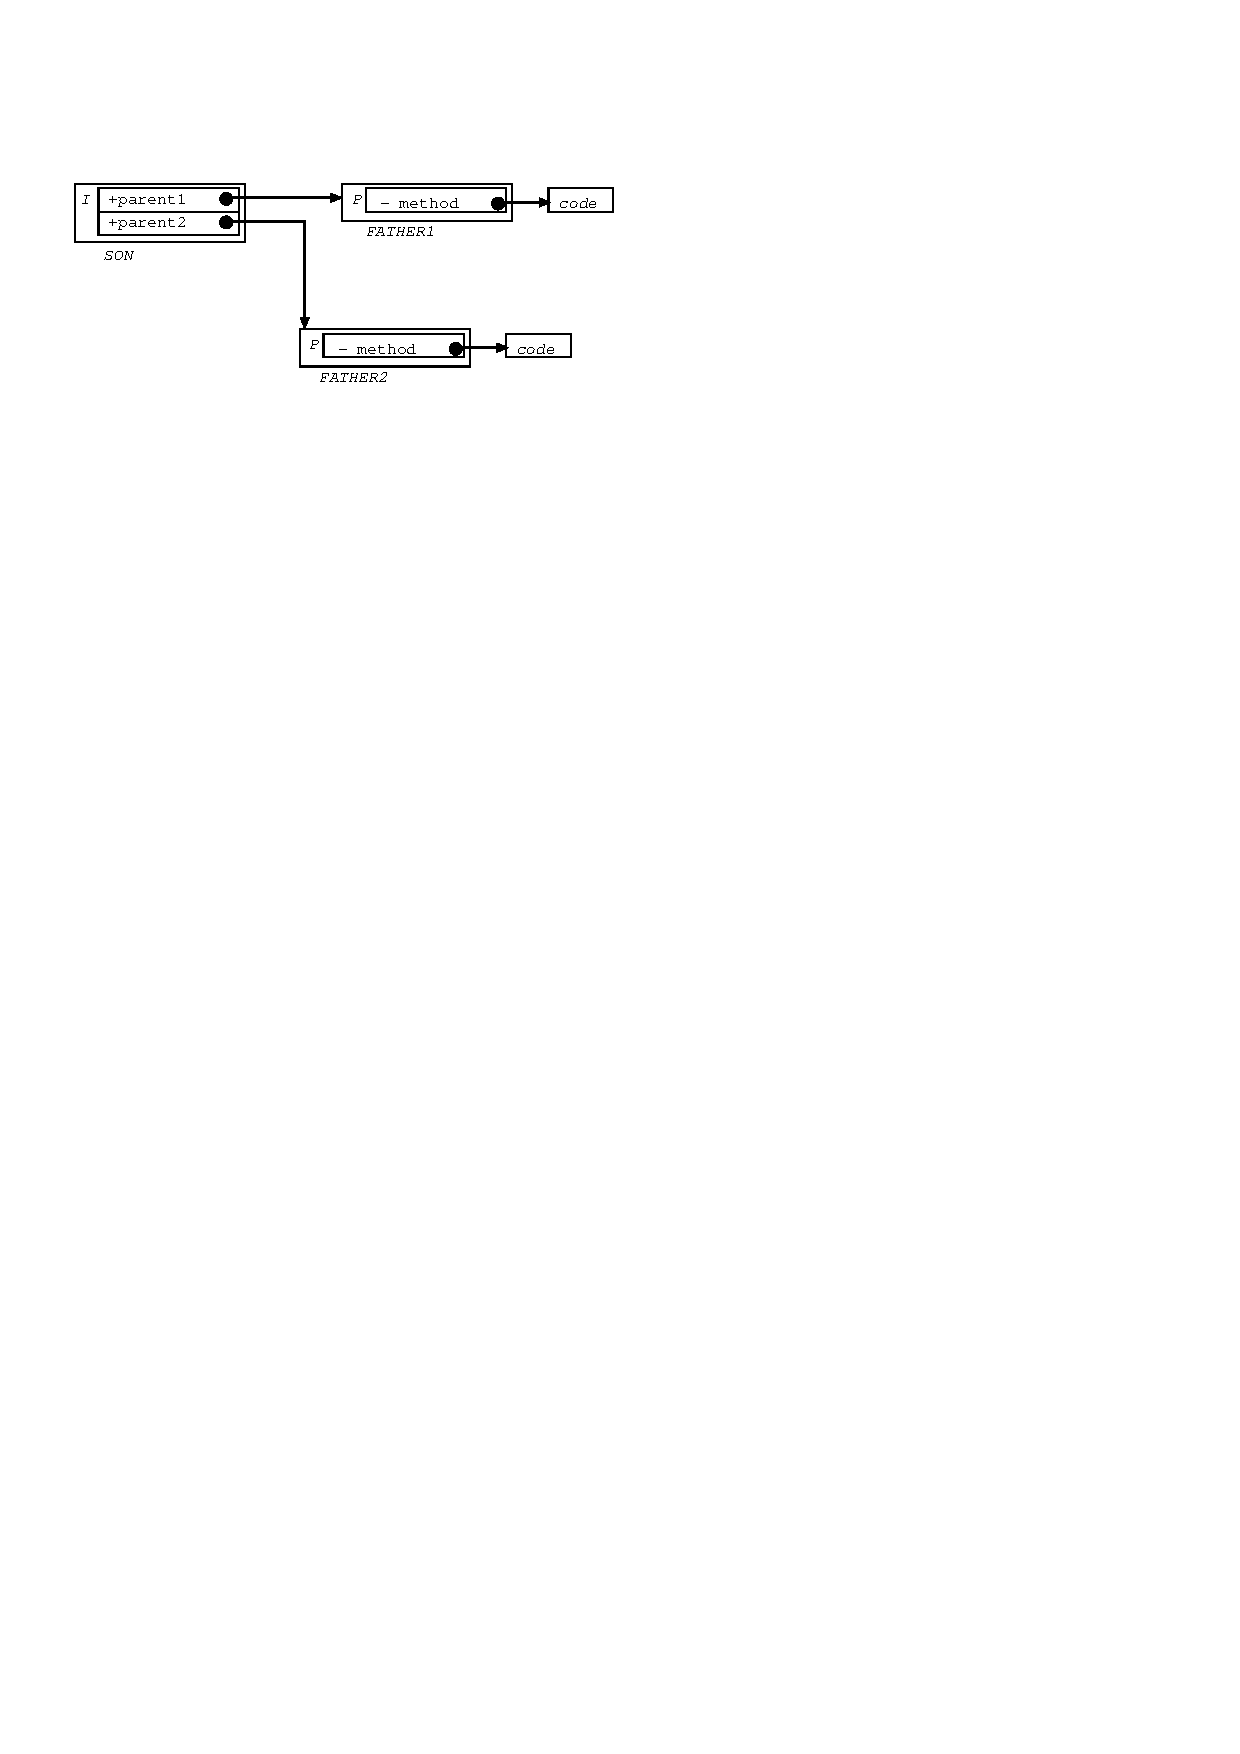
\includegraphics[scale=1.0]{figures/resend}
\end{center}
{\tt{}{\bf{}method};}
\begin{center}
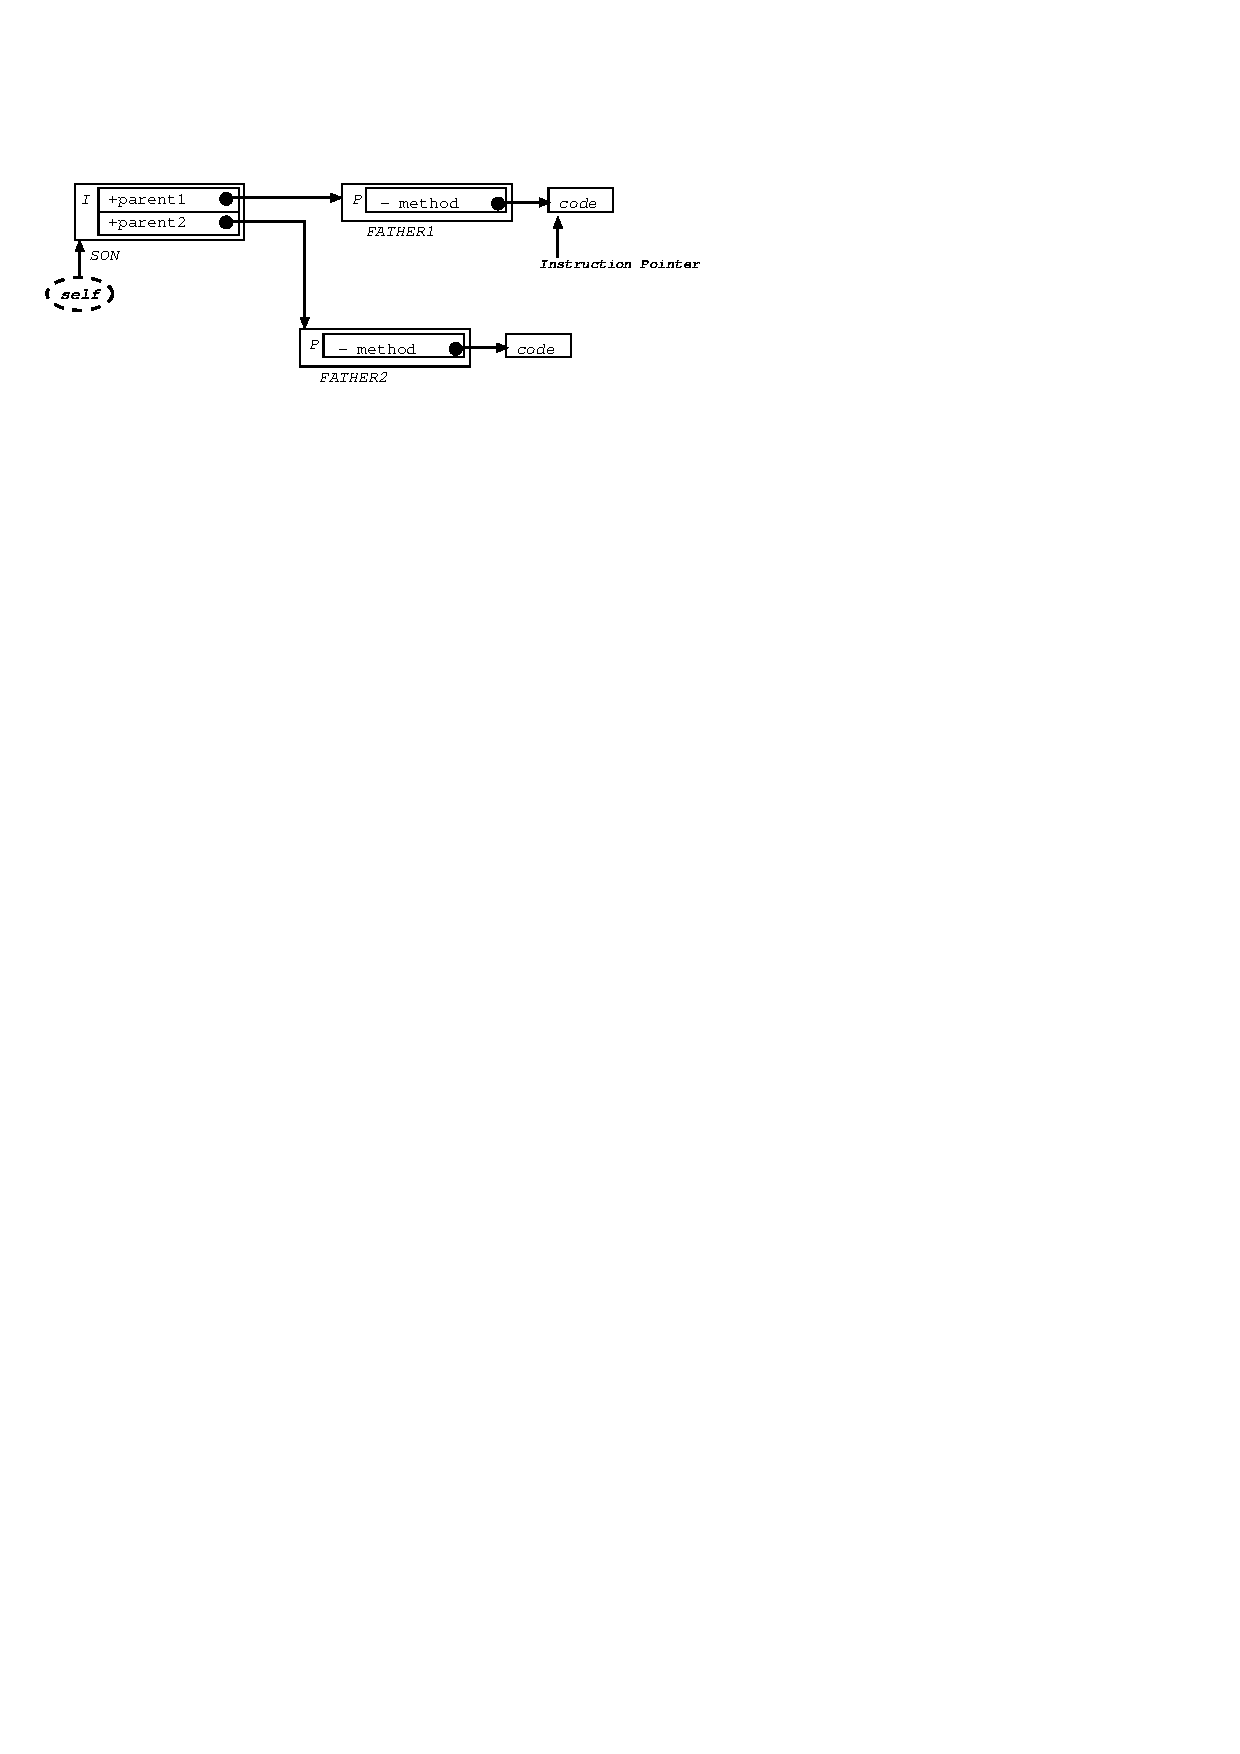
\includegraphics[scale=1.0]{figures/resend1}
\end{center}
{\tt{}{\bf{}parent2.method};}
\begin{center}
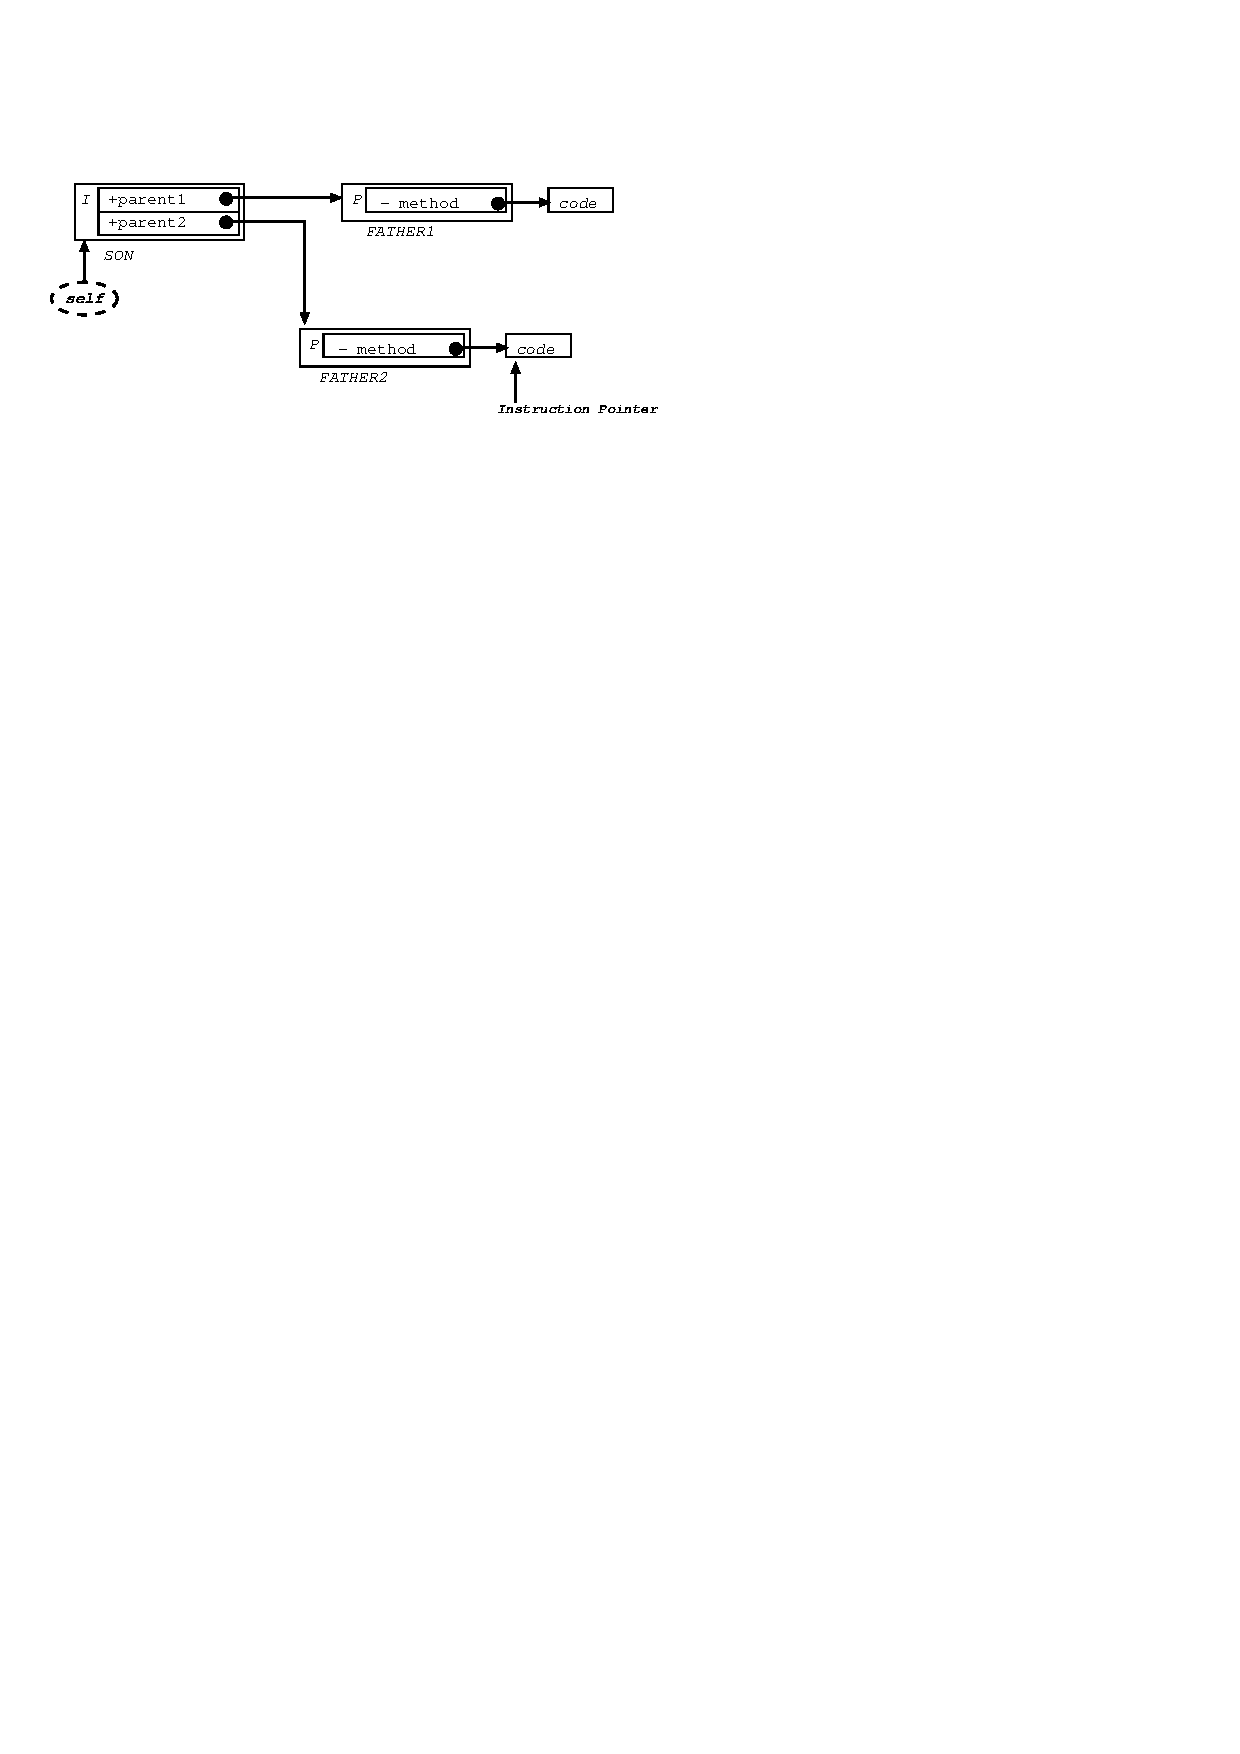
\includegraphics[scale=1.0]{figures/resend2}
\end{center}

%--------------------------------------------------------
\subsection{The {\tt{}Insert} section }
\label{language_reference:section_identifiers:insert_section}
%--------------------------------------------------------

Slots defined in an Insert section are almost equivalent to Inheritence slots.
The difference resides in the fact that the return type is not a parent of your
prototype. In other words, your prototype isn't a sub-type of a slot's return type
residing in section Insert.

Note 1: Expanded prototypes can only use section Insert, not the Inherit section.

Note 2: The slots order is important regarding the search (lookup algorythm) of a message. 
You can put as many Inherit or Insert sections at the beginning of your prototype.

%--------------------------------------------------------
\subsection{The {\tt{}Mapping} section }
\label{language_reference:section_identifiers:mapping_section}
%--------------------------------------------------------
\index{Section Mapping}
\index{Mapping}
The Mapping section purpose is to format data slots description according to some fixed hardware data structure. \\
In such a section, the compiler follows exactly the order and the description of slots as they are written to map exactly the
corresponding hardware data structure.\\
Thus, one is able to write data slots description according to the hardware to handle.\\
You can only define slots with the {\bf{} +} symbol, and only datas (not code).\\
Otherwise, these attributes are used exactly as the others not in the mapping section (reading or writting).
\begin{alltt}
{\bf{}Section Mapping}
  + {\bf{}x1}:{\sc{}uinteger\_32};   // 4 bytes, unsigned
  + {\bf{}x2}:{\sc{}uinteger\_8};    // 1 byte,  unsigned
  + {\bf{}x3}:{\sc{}integer\_8};     // 1 byte,  signed
  + {\bf{}x4}:{\sc{}uinteger\_16};   // 2 bytes, unsigned
  + {\bf{}x5}:{\sc{}integer\_32};    // 4 bytes, signed
  + {\bf{}x6}:{\sc{}integer\_16};    // 2 bytes, signed 
  + {\bf{}x7}:{\sc{}uinteger\_16};   // 2 bytes, unsigned
\end{alltt}
These prototype match exactly a 16 byte physical structure.
\begin{center}
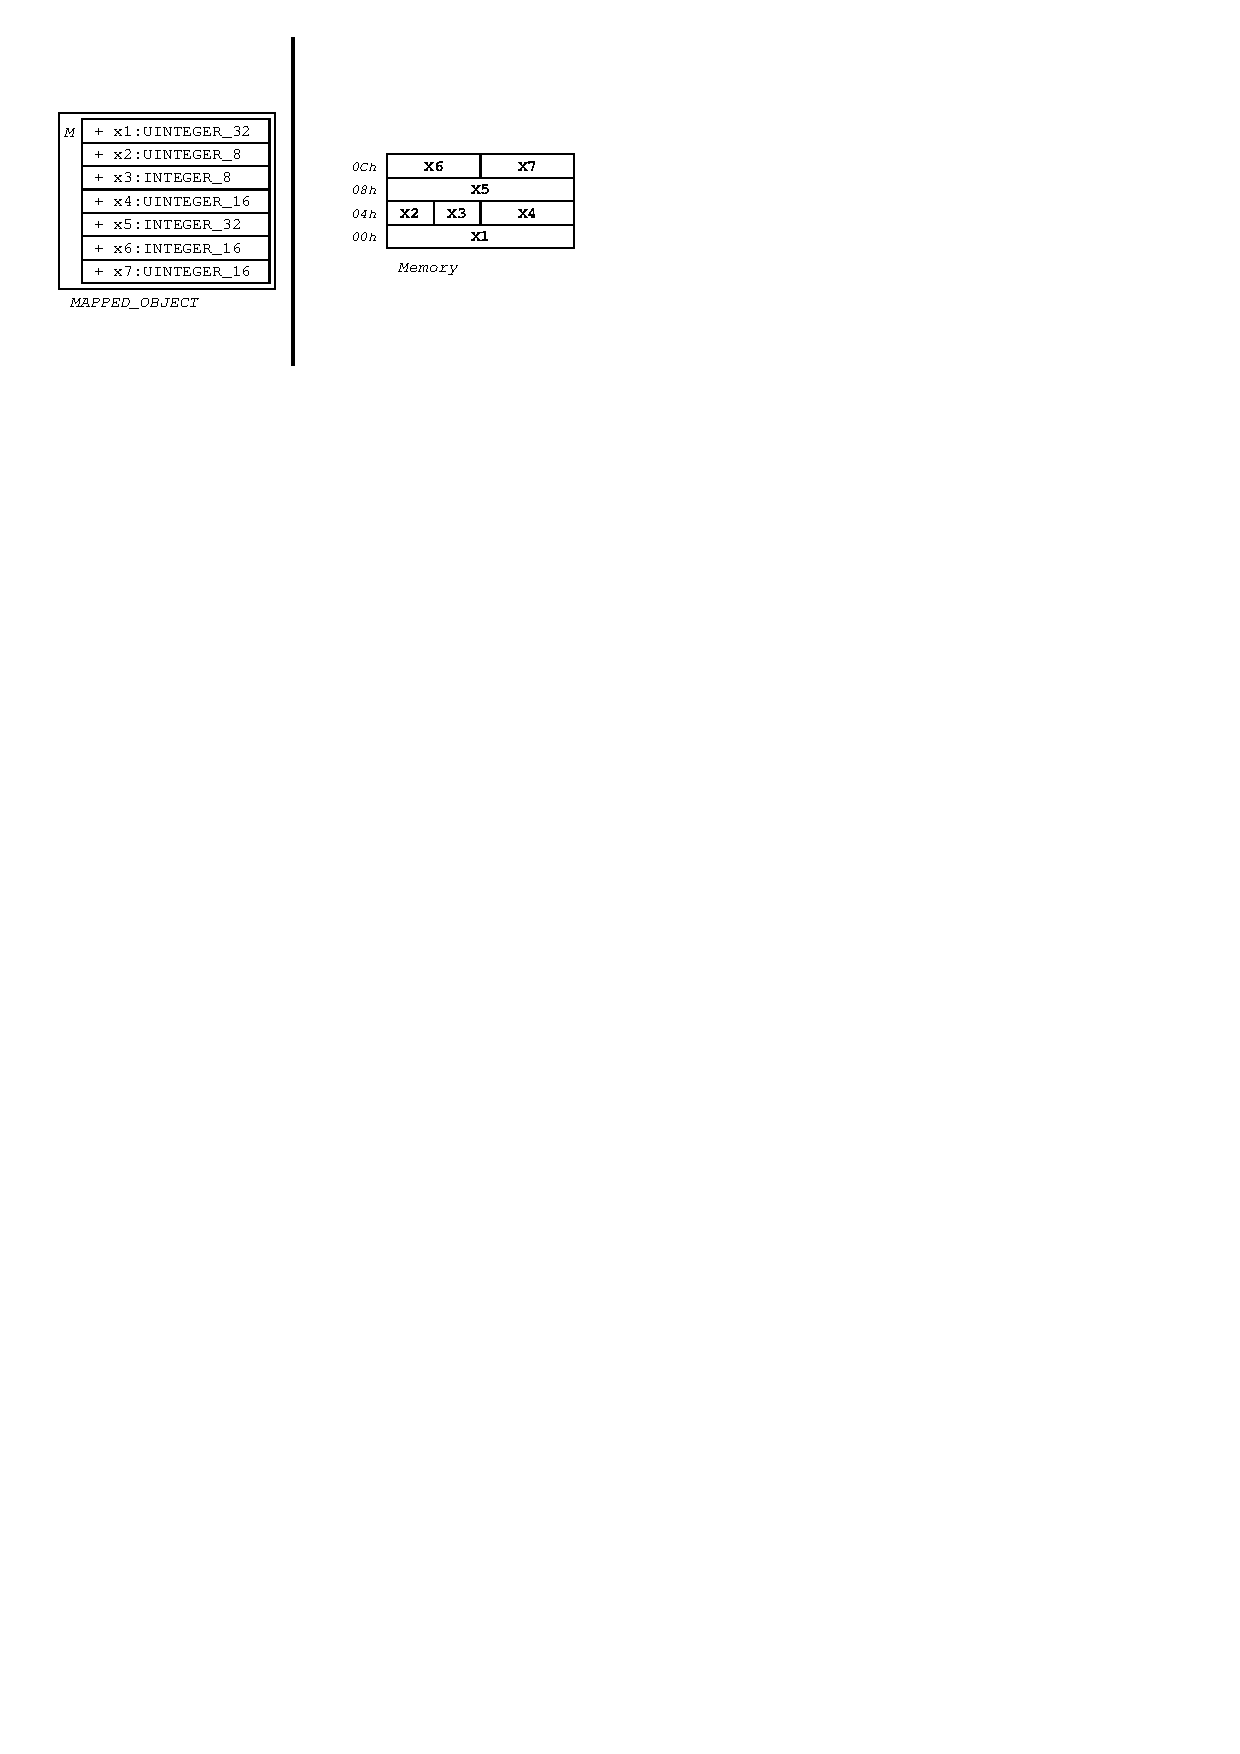
\includegraphics[scale=1.0]{figures/mapping}
\end{center}

\warning{} Slots inside some Mapping section are considered private for any other objects.
Slots can only be defined with the {\bf{}+} property. No slot outside this section can be defined with the {\bf{}+} property.\\
\begin{alltt}
{\bf{}Section Mapping}
  + {\bf{}x1}:{\sc{}ushortint};   
  - {\bf{}x2}:{\sc{}uinteger};          // Compiler will stop in error
{\bf{}Section Public}
  + {\bf{}count}:{\sc{}integer} := 3;   // Compiler will stop in error
  - {\bf{}slot}:{\sc{}integer} <- /* \ldots */ // Ok
\end{alltt}

The mapping can also be used to represent files.
%---------------------------------------------------------
\subsection{The {\tt{}Interrupt} section }
\label{language_reference:section_identifiers:interrupt_section}
%---------------------------------------------------------
\index{Section Interrupt}
\index{Interruption}
The goal of the Interrupt section is to handle hardware interruptions.\\
In this section you can define methods (code slots) that will be
executed only while there is an interrupt associated.\\  
Each slot is associated with one of the processor's interruptions \cite{bookpc00}.\\
These slots differ from others in their generated code. For example,
their entry and exit codes are related to the interrupt processing.\\ 
Their invocations are asynchronous and borrow the quantum of the
current process.\\ 
Generally, these slots are little time consumers and they don't
require specific process' context for their executions.\\ 
It is thus necessary to be careful while programming such slots to
ensure the consistency of the interrupted process.\\ 

Define your method (without return value, because you don't explicitly call it) as any other classical method.\\
Then associate the adress of your method with the effective interrupt jump adress (it depends on your architecture). This can be done using a system mapped object.\\
When your interrupt physically happens, there is the call of your associated method, which returns a pointer on the code.\\
The compiler will not optimize local variables of your interrupt method because of its particularity: the call depends on the context and cannot be anticipated during compilation.
\begin{alltt}
{\bf{}Section Interrupt}
  - {\bf{}interrupt\_01} <- /* \ldots */;
\end{alltt} 
\begin{center}
\includegraphics[scale=1.0]{figures/interrupt}
\end{center}
You must define as C external (\ref{language_reference:externals} page \pageref{language_reference:externals}) the following macros: {\sc{}\_\_begin\_interrupt\_\_} and {\sc{}\_\_end\_interrupt\_\_}.
These macros will be executed every time an interrupt function is activated.
The code of these macros depends on the architecture.
Example for X86 follows.
\begin{alltt}
{\bf{}Section Header}
  + {\bf{}name} := {\sc{}interrupt\_manager};
  - {\bf{}category} := {\sc{}kernel};
  - {\bf{}external} := `  
#define __BEGIN_INTERRUPT__ volatile unsigned long eax;
  volatile unsigned long ebx;
  volatile unsigned long ecx;
  volatile unsigned long edx;
  volatile unsigned long esi;
  volatile unsigned long edi;
                             
  asm volatile (
  "/* BEGIN INTERRUPT */
  movl %%eax,%0
  movl %%ebx,%1
  movl %%ecx,%2
  movl %%edx,%3
  movl %%esi,%4
  movl %%edi,%5
  /* BEGIN CODE */"
  : "=m"(eax),"=m"(ebx),"=m"(ecx),"=m"(edx),"=m"(esi),"=m"(edi)
  : /* no input */
  : "eax","edx","ecx","ebx","ebp","esi","edi", "memory");

#define __END_INTERRUPT__ asm volatile (
 "/* END CODE */ 
  movl %0,%%eax
  movl %1,%%ebx
  movl %2,%%ecx
  movl %3,%%edx
  movl %4,%%esi
  movl %5,%%edi
  movl %%ebp,%%esp
  popl %%ebp      
  iret            
 /* END INTERRUPT */"
 : /* no output */ 
 : "m"(eax),"m"(ebx),"m"(ecx),"m"(edx),"m"(esi),"m"(edi)
 : "eax","edx","ecx","ebx","ebp","esi","edi", "memory");

`;
\end{alltt}

%---------------------------------------------------------
\subsection{The External section }
\label{language_reference:section_identifiers:external_section}
%---------------------------------------------------------
\index{Section External}
\index{External}
When a slot is define in Lisaac, its real name (the name of the slot after compilation) is different in the produced C code because of the compiler (optimization, specialization, \ldots).

You can define a special section, {\bf{}Section External}, which specified that the function here define must keep their name after compilation.This capability is very useful when you want to link the produced C code with existing code.

This section is more detailed in section {\ref{language_reference:externals} page \pageref{language_reference:externals}}.

%---------------------------------------------------------
\subsection{Other sections}
\label{language_reference:section_identifiers:other_section}
%---------------------------------------------------------
\index{Section, other}
%
Other sections shared the same objective: they all are section of code and datas.
The difference between these sections are only the visibility of their slot (method and datas).
There is 4 kind of sections of this type:
the {\bf{}Private} section, the {\bf{}Public} section, the {\bf{}Directory} and the {\it{}prototype list} section.
\paragraph{{\bf{}Section Private}} \index{Section Private} \index{Private, section}
~\\
It's the most restrictive section. The slots defined in it are only accessibles inside the current object (the {\it{}self} object) but not for its descendants.

{\bf{}Section Interrupt}, {\bf{}Section Mapping} and {\bf{}Section Inherit} are considered {\bf{}Private}.

\paragraph{{\bf{}Section SELF}} \index{Section SELF} \index{SELF, section}
~\\
The slots defined in it are only accessible inside the current object but also for its descendants. Note that its the keyword {\sc{}self} is written in capital, which is a different as other keywords.

\paragraph{{\bf{}Section} {\it{}prototype list}} \index{Section {\it{}prototype list}}
~\\
This section is defined with the keyword {\bf{}Section} followed by a list of prototypes (in capital, separated by {\bf,}) which are allowed to call the slots (example: {\bf{}Section} {\sc{}integer,boolean,string}). The {\it{}self} object has also the right to call it.

\paragraph{{\bf{}Section Directory}} \index{Section Directory}
~\\
This type of section gives access to all prototypes contained in the same directory as your prototype.
Prototypes contained in a sub-directory also have access to these slots. It permits easy access securisation
while organizing your prototypes into directories and sub-directories.

\paragraph{{\bf{}Section Public}} \index{Section Public} \index{Public}
~\\
It's the most permitive section. The slots defined in it are accessibles from all the objects.\\

You can define as many sections as you want.

\begin{alltt} 
{\bf{}Section Header}
  + {\bf{}name} := {\sc{}first};

{\bf{}Section Private}
  + {\bf{}slot\_private} <- /* \ldots */
{\bf{}Section SELF}
  + {\bf{}slot\_self} <- /* \ldots */
{\bf{}Section} {\sc{}first}
  + {\bf{}slot\_list1} <- /* \ldots */
{\bf{}Section} {\sc{}first,second}
  + {\bf{}slot\_list2} <- /* \ldots */
{\bf{}Section Public}
  + {\bf{}slot\_public}  <- /* \ldots */
\end{alltt}

\noindent
\begin{tabularx}{\textwidth}{X c c c c c}
\hline
{\bf{}Object} & {\bf{}slot\_private} & {\bf{}slot\_self} & {\bf{}slot\_list1} & {\bf{}slot\_list2} & {\bf{}slot\_public}\\
\hline
\hline
{{\it{}self} object only, Not its descendants} & {\sc{}OK} & {\sc{}OK} & {\sc{}OK} & {\sc{}OK} & {\sc{}OK} \\
\hline
{{\it{}self} object and its descendants} & {\sc{}X}  & {\sc{}OK} & {\sc{}OK} & {\sc{}OK} & {\sc{}OK} \\
\hline
{Type {\sc{}first} ('master' object {\sc{}first} all its clones and descendants)} & {\sc{}X}  & {\sc{}X}  & {\sc{}OK} & {\sc{}OK} & {\sc{}OK}\\
\hline
{Type {\sc{}second} ('master' object {\sc{}second} all its clones and descendants)} & {\sc{}X}  & {\sc{}X}  & {\sc{}OK} & {\sc{}OK} & {\sc{}OK}\\
\hline
Any type except {\sc{}first} and {\sc{}second}    & {\sc{}X} & {\sc{}X}& {\sc{}X} & {\sc{}X} & {\sc{}OK} \\
\hline
\end{tabularx}


\noindent 
Examine this example in details:
\begin{alltt} 
{\bf{}Section Header}
  + {\bf{}name} := {\sc{}first};

{\bf{}Section Private}
  + {\bf{}slot\_private} <- /* \ldots */
{\bf{}Section SELF}
  + {\bf{}slot\_self} <- /* \ldots */
{\bf{}Section} {\sc{}first}
  + {\bf{}slot\_list1} <- /* \ldots */
{\bf{}Section} {\sc{}first,second}
  + {\bf{}slot\_list2} <- /* \ldots */
{\bf{}Section Public}
  + {\bf{}slot\_public}  <- /* \ldots */

  + {\bf{}slot\_test} <-
  (
    {\bf{}slot\_private};     // Allowed
    {\bf{}slot\_self};        // Allowed
    {\bf{}slot\_list1};       // Allowed
    {\bf{}slot\_list2};       // Allowed
    {\bf{}slot\_public};      // Allowed        
  );

  + {\bf{}slot\_test2} <-
  ( + object\_first:{\sc{}first};
    object\_first := {\sc{}first}.{\bf{}clone};
    object\_first.{\bf{}slot\_private};     // Forbidden
    object\_first.{\bf{}slot\_self};        // Forbidden
    object\_first.{\bf{}slot\_list1};       // Allowed
    object\_first.{\bf{}slot\_list2};       // Allowed
    object\_first.{\bf{}public};            // Allowed        
  );\\

{\bf{}Section Header}
  + {\bf{}name} := {\sc{}second};

{\bf{}Section Public}
  + {\bf{}slot\_test} <-
  ( + object\_first:{\sc{}first};
    object\_first := {\sc{}first}.{\bf{}clone};
    object\_first.{\bf{}slot\_private};     // Forbidden
    object\_first.{\bf{}slot\_self};        // Forbidden
    object\_first.{\bf{}slot\_list1};       // Forbidden
    object\_first.{\bf{}slot\_list2};       // Allowed
    object\_first.{\bf{}public};         // Allowed        
  );\\

{\bf{}Section Header}
  + {\bf{}name} := {\sc{}other};

{\bf{}Section Public}
  + {\bf{}slot\_test} <-
  ( + object\_first:{\sc{}first};
    object\_first := {\sc{}first}.{\bf{}clone};
    object\_first.{\bf{}slot\_private};     // Forbidden
    object\_first.{\bf{}slot\_self};        // Forbidden
    object\_first.{\bf{}slot\_list1};       // Forbidden
    object\_first.{\bf{}slot\_list2};       // Forbidden
    object\_first.{\bf{}public};         // Allowed        
  );
\end{alltt}

\warning{} The call of a slot in {\bf{}Section Private} or {\bf{}Section SELF} is restricted to the implicit call. You can't use the {\bf{}Self} object.
\begin{alltt}
{\bf{}Section Header}
  + {\bf{}name} := {\sc{}first};

{\bf{}Section Private}
  + {\bf{}slot\_private} <- /* \ldots */
{\bf{}Section SELF}
  + {\bf{}slot\_self} <- /* \ldots */
{\bf{}Section Public}
  + {\bf{}slot\_test} <-
  (
    {\bf{}slot\_private};              // Allowed
    {\bf{}slot\_self};                 // Allowed
    {\bf{}Self}.{\bf{}slot\_private};   // Forbidden
    {\bf{}Self}.{\bf{}slot\_self};      // Forbidden
  );
\end{alltt} 

\paragraph{Accessibility and inheritance} \index{Inheritance, accessibility}
~\\
Inheritance share the same accessibility between parents and sons.
For example, if a slot is defined in a {\bf{}Public} section in a parent, it is also {\bf{}Public} for its descendants.
Note that a {\bf{}Private} slot is not visible from the descendants.
If you define a visibility for a prototype, it is also available for its descendants.
Look at the accessibility as if the considered slot was effectively in the current object and not in its parents.
\begin{alltt} 
{\bf{}Section Header}
  + {\bf{}name} := {\sc{}father};

{\bf{}Section Private}
  + {\bf{}slot\_private} <- /* \ldots */
{\bf{}Section SELF}
  + {\bf{}slot\_self} <- /* \ldots */
{\bf{}Section} {\sc{}father}
  + {\bf{}slot\_list1} <- /* \ldots */
{\bf{}Section} {\sc{}first}
  + {\bf{}slot\_list2} <- /* \ldots */\\

{\bf{}Section Header}
  + {\bf{}name} := {\sc{}son};

{\bf{}Section Inherit}
  + {\bf{}parent}:{\sc{}father} := {\sc{}father};
{\bf{}Section Public}
  + {\bf{}slot\_test} <-
  ( 
    {\bf{}slot\_private};                      // Forbidden
    {\bf{}slot\_self};                         // Allowed
    {\bf{}slot\_list1};                        // Allowed ({\sc{}father} and all its descendants)
    {\bf{}slot\_list2};                        // Forbidden
  );

  + {\bf{}slot\_test2} <-
  ( + object\_son:{\sc{}son};
    object\_son := {\sc{}son}.{\bf{}clone};
    object\_son.{\bf{}slot\_private};          // Forbidden
    object\_son.{\bf{}slot\_self};             // Forbidden
    object\_son.{\bf{}slot\_list1};            // Allowed
    object\_son.{\bf{}slot\_list2};            // Forbidden
  );\\

{\bf{}Section Header}
  + {\bf{}name} := {\sc{}first};

{\bf{}Section Public}
  + {\bf{}slot\_test} <-
  ( + object\_son:{\sc{}son};
    object\_son := {\sc{}son}.{\bf{}clone};
    object\_son.{\bf{}slot\_private};          // Forbidden
    object\_son.{\bf{}slot\_self};             // Forbidden
    object\_son.{\bf{}slot\_list1};            // Forbidden
    object\_son.{\bf{}slot\_list2};            // Allowed
  );
\end{alltt}

Accessibility restricted to a prototype is also valid for its descendants.
In the previous example, call on slot\_list2 is allowed in all the objects of {\sc{}first} type and for all its descendants.
\begin{alltt}
{\bf{}Section Header}
  + {\bf{}name} := {\sc{}son\_first};

{\bf{}Section Inherit}
  + {\bf{}parent}:{\sc{}first} := {\sc{}first};
{\bf{}Section Public}
  + {\bf{}slot\_test} <-
  ( + object\_son:{\sc{}son};
    object\_son := {\sc{}son}.{\bf{}clone};
    object\_son.{\bf{}slot\_private};          // Forbidden
    object\_son.{\bf{}slot\_self};             // Forbidden
    object\_son.{\bf{}slot\_list1};            // Forbidden
    object\_son.{\bf{}slot\_list2};            // Allowed
  );
\end{alltt}

You must also keep the same accesibility type when you redefine a slot in a son.

\begin{alltt} 
{\bf{}Section Header}
  + {\bf{}name} := {\sc{}father};

{\bf{}Section Private}
  + {\bf{}slot\_private} <- /* \ldots */
{\bf{}Section} {\sc{}first}
  + {\bf{}slot\_list1} <- /* \ldots */\\

{\bf{}Section Header}
  + {\bf{}name} := {\sc{}son};

{\bf{}Section Inherit}
  + {\bf{}parent}:{\sc{}father} := {\sc{}father};
{\bf{}Section Private}
  + {\bf{}slot\_private} <- /* \ldots */   // Ok, it respects the same accessibility
{\bf{}Section} Public
  + {\bf{}slot\_list1} <- // Error: accessibility is different between {\sc{}father} and {\sc{}son}
  /* \ldots */ 
\end{alltt}


%=========================================================
\section{Type names}
\label{language_reference:type_names}
%=========================================================
%
\index{Type}
Type names are noted with prototype names.
A keyword in uppercase (capital letter) identify them.
\begin{alltt} 
  + {\bf{}color}:{\sc{}integer};
\end{alltt}
%--------------------------------------------------------
\subsection{Genericity}
\label{language_reference:type_names:genericity}
%--------------------------------------------------------
\index{Genericity}
\index{Type, Genericity}

To ease the implementation of containers like arrays, linked
lists and dictionaries for example, we also added a form of genericity
(parametric types) such as the one defined in Eiffel \cite{meyer94a}.
\begin{alltt}
  + {\bf{}array}:{\sc{}array}({\sc{}character});
\end{alltt}
To define such a prototype using genericity, you'll define between '(' and ')' the abstract types used, 
separated by commas ',' or by keywords. In the definitions of slots, you can use your abstract type
\begin{alltt}
{\bf{}Section Header}
  + {\bf{}name} := {\sc{}genericity\_example}({\sc{}e},{\sc{}f});

{\bf{}Section Public}
  - {\bf{}slot}:{\sc{}f} <-
  ( + elt:{\sc{}e};
    /* \ldots */
  );
\end{alltt}
\warning{} The name of the prototype is the entire name, with '(' and ')'.
\begin{alltt}
{\bf{}Section Header}
  + {\bf{}name} := {\sc{}test};

{\bf{}Section Public}
  - {\bf{}slot} <-
  ( + gen:{\sc{}genericity\_example};     // Error: the type does not exist
    + gen2:{\sc{}genericity\_example}({\sc{}string},{\sc{}integer});  // OK
    /* \ldots */
  );
\end{alltt}
Note that when you use the genericity-prototype, you have to precise the real types you want.


%--------------------------------------------------------
\subsection{Invariant's type control}
\label{language_reference:type_names:invariant}
%--------------------------------------------------------
\index{Type, invariant}
\index{Invariant, type}
The redefinition of a slot must have the same profile as her
parent (standard type and name for the arguments and the return value).

\begin{alltt}
{\bf{}Section Header}
  + {\bf{}name} := {\sc{}father};

{\bf{}Section Public}
  + {\bf{}to\_string} arg:{\sc{}integer} :{\sc{}string} <- /* \ldots */\\

{\bf{}Section Header}
  + {\bf{}name} := {\sc{}son};

 {\bf{}Section Inherit}
  - {\bf{}parent}: {\sc{}father}:= {\sc{}father};
{\bf{}Section Public}
  + {\bf{}to\_string} arg:{\sc{}integer} :{\sc{}string} <- /* \ldots */ // Ok, follow the same profile\\

{\bf{}Section Header}
  + {\bf{}name} := {\sc{}son};

{\bf{}Section Inherit}
  - {\bf{}parent}:{\sc{}father} := {\sc{}father};
{\bf{}Section Public}
  + {\bf{}to\_string} arg:{\sc{}real} :{\sc{}array(character)} <- // Error: not the same profile
  /* \ldots */ 
\end{alltt}

%--------------------------------------------------------
\subsection{Particular type: {\sc{}self} type}
\label{language_reference:type_names:self}
%--------------------------------------------------------
%
\index{SELF, prototype}
\index{Type, SELF}
The type {\sc{}self} represents a prototype which is exactly 
the same type as the current prototype.

\begin{alltt}
{\bf{}Section Header}
  + {\bf{}name} := {\sc{}example};

{\bf{}Section Public}
  + {\bf{}slot}:{\sc{}self} <- ( /* \ldots */ );
\end{alltt}

Here the {\sc{}self} type is exactly {\sc{}example}.

Another example using inheritance:
\begin{alltt}
{\bf{}Section Header}
  + {\bf{}name} := {\sc{}father};

{\bf{}Section Public}
  - {\bf{}create}:{\sc{}self} <- 
  ( + result:{\sc{}self};
    result := {\sc{}self}.clone;
    result
  );\\

{\bf{}Section Header}
  + {\bf{}name} := {\sc{}son};

{\bf{}Section Inherit}
  - {\bf{}parent}:{\sc{}father} := {\sc{}father};\\

{\bf{}Section Header}
  + {\bf{}name} := {\sc{}test};

{\bf{}Section Public}
  - {\bf{}main}:=
  ( + object\_father:{\sc{}father};
    + object\_son:{\sc{}son};
    object\_father := {\sc{}father}.{\bf{}create};  // Type {\sc{}father}
    object\_son := {\sc{}son}.{\bf{}create};        // Type {\sc{}son}
  );
\end{alltt}
We can see with this last example that even if the slot which returns {\sc{}self} type is defined in a parent, it's the current object which define the real type of {\sc{}self}.

\warning{} {\sc{}self} type is available only if the result is calculated.
You can't write
\begin{alltt}
  - {\bf{}slot}:{\sc{}self};
\end{alltt}
Because if you have inheritance and the slot {\sc{}self} in the parent, in the children the type is different.

\begin{alltt}
{\bf{}Section Header}
  + {\bf{}name} := {\sc{}father};

{\bf{}Section Public}
  - {\bf{}a}:{\sc{}self};\\

{\bf{}Section Header}
  + {\bf{}name} := {\sc{}son1};

{\bf{}Section Inherit}
  - {\bf{}parent}:{\sc{}father} := {\sc{}father};
{\bf{}Section Public}
  - {\bf{}affect\_a} <- ( {\bf{}a} := {\sc{}self}; );  // Here {\sc{}self} is {\sc{}son1}

{\bf{}Section Header}
  + {\bf{}name} := {\sc{}son2};

{\bf{}Section Inherit}
  - {\bf{}parent}:{\sc{}father} := {\sc{}father};
{\bf{}Section Public}
  - {\bf{}affect\_a} <- ( {\bf{}a} := {\sc{}self}; );  // Here {\sc{}self} is {\sc{}son1}\\

{\bf{}Section Header}
  + {\bf{}name} := {\sc{}test};

{\bf{}Section Public}
  - {\bf{}main} :=
  ( + object_son1:{\sc{}son1};
    + object_son2:{\sc{}son2};
    object_son1 := {\sc{}son1}.{\bf{}clone};
    object_son2 := {\sc{}son2}.{\bf{}clone};
    object_son1.{\bf{}affect\_a};  // Ok
    object_son2.{\bf{}affect\_a};  // Error of typing, {\bf{}a} is type {\sc{}son1}
                                   // and can't be then {\sc{}son2}
  );
\end{alltt}

%--------------------------------------------------------
\subsection{Particular type: {\sc{}fixed\_array(e)} type}
\label{language_reference:type_names:fixed_array}
%--------------------------------------------------------
%
\index{Type FIXED\_ARRAY[E]}
\index{List, FIXED\_ARRAY[E]}
The {\sc{}fixed\_array(e)} type is the object representation of a values' vector.

\begin{alltt}
  + my\_vector:{\sc{}fixed\_array(integer)};

  my\_vector := (0, 1);       // It's one vector with 2 values.
  my\_vector := (0, 1, 2, 3); // It's one vector with 4 values.
\end{alltt}

The prototype {\sc{}fixed\_array(e)} becomes a non-mutable collection (static)

%========================================================
\section{Prefix of types}
\label{language_reference:prefix_types}
%========================================================
\index{Type, Prefix}

%---------------------------------------------------------
\subsection{{\tt{}Expanded} type}
\label{language_reference:type_names:expanded_type}
%---------------------------------------------------------
\index{Type, Expanded}
\index{Expanded type}
If the slots use the keyword {\bf{}Expanded}, its value is cloned and embedded (in memory) in the prototype.
The keyword can be used either with {\bf{}+} or {\bf{}-} (see \ref{language_reference:slots:expanded_slots}).
If the slot {\tt{}name} of a prototype is followed by {\tt{}Expanded}, slots of this type are automatically
{\tt{}Expanded}.

For example\,:\\
\begin{alltt}
{\bf{}Section Header}
  + {\bf{}name} := {\bf{}Expanded} {\sc{}foo};

{\bf{}Section Public}
  - {\bf{}slot\_foo}:{\sc{}foo}; // <=> Expanded {\sc{}foo}
\end{alltt}

%---------------------------------------------------------
\subsection{{\tt{}Strict} type}
\label{language_reference:type_names:strict_type}
%---------------------------------------------------------
\index{Type, Strict}
\index{Strict type}

If a slot use the keyword {\bf{}Strict}, its value is exactly this type.
You can't affect this slot with a son of the same type. It establish a strong restriction
permitting exchange and manipulation between referenced and expanded objects
(see \ref{language_reference:type_names:strict_type}). {\bf{}Strict} can only be used on reference objects.
{\bf{}Strict Expanded} is therefore illegal.

If the slot {\tt{}name} of a prototype is defined with the {\tt{}Strict} word, slots of this type are 
automatically {\tt{}Strict}.

For example\,:\\
\begin{alltt}
{\bf{}Section Header}
  + {\bf{}name} := {\bf{}Strict} {\sc{}foo};

{\bf{}Section Public}
  - {\bf{}slot\_foo}:{\sc{}foo}; // <=> Strict {\sc{}foo}
\end{alltt}

%========================================================
\section{Slots}
\label{language_reference:slots}
%========================================================
\index{Slot}

%---------------------------------------------------------
\subsection{Default value of a slot according to its type.}
\label{language_reference:type_names:default}
%---------------------------------------------------------
%
\index{Default value}
A default value can also be defined in the slot {\bf{}default} in the {\bf{}Section Header}.
It can be a value or an expression evaluated at initialisation of the slot or the local slot (at start of execution of the method).

\begin{alltt} 
{\bf{}Section Header}
  + {\bf{}name} := {\sc{}example};

  - {\bf{}default}:= {\sc{}null};
\end{alltt}

If you use the prototype without initializing it, its value will be {\sc{}null}.

%--------------------------------------------------------
\subsection{Shared slots}
\label{language_reference:slots:shared_slots}
%--------------------------------------------------------
\index{Slot, shared}
If the slot is preceded by the {\bf{}-} character, its value is shared between all the clones of the prototype (global slot).
\paragraph{Overview}
 ~\\
\begin{alltt}
{\bf{}Section Header}
  + {\bf{}name} := {\sc{}foo};

{\bf{}Section Public}
  - {\bf{}slot\_foo}:{\sc{}integer} := 5;\\

{\bf{}Section Header}
  + {\bf{}name} := {\sc{}example};

{\bf{}Section Public}
  - {\bf{}slot1}:{\sc{}integer} := 3;
  - {\bf{}slot2}:{\sc{}foo} := {\sc{}foo};
\end{alltt}

\begin{center}
\includegraphics[scale=1.0]{figures/shared_slot}
\end{center}

The difference between {\bf{}slot1} and {\bf{}slot2} is that {\sc{}integer} is {\bf{}Expanded}.
We will see this in section {\ref{language_reference:slots:expanded_slots}} page \pageref{language_reference:slots:expanded_slots}.

Note that the 2 objects shared the same pointer on the {\sc{}foo} object. So if you change the pointer, it changes for all the clones.

Non expanded objects have their default value set to {\sc{}null}.

\begin{alltt}
{\bf{}Section Header}
  + {\bf{}name} := {\sc{}foo};

{\bf{}Section Public}
  - {\bf{}slot\_foo}:{\sc{}integer} := 5;\\

{\bf{}Section Header}
  + {\bf{}name} := {\sc{}example};

{\bf{}Section Public}
  - {\bf{}slot1}:{\sc{}integer};
  - {\bf{}slot2}:{\sc{}foo};
\end{alltt}

\begin{center}
\includegraphics[scale=1.0]{figures/shared_slot2}
\end{center}

\paragraph{Assignment} \index{Slot, assignment} \index{Assignment, slot}
~\\
\begin{alltt}
{\bf{}Section Header}
  + {\bf{}name} := {\sc{}foo};

{\bf{}Section Public}
  - {\bf{}slot\_foo}:{\sc{}integer} := 5;\\

{\bf{}Section Header}
  + {\bf{}name} := {\sc{}example};

{\bf{}Section Public}
  - {\bf{}slot1}:{\sc{}integer};
  - {\bf{}slot2}:{\sc{}foo};
  - {\bf{}inc\_slot1} <- ( {\bf{}slot1} := {\bf{}slot1} + 1; );
  - {\bf{}set\_slot2} f:{\sc{}foo} <- ( {\bf{}slot2} := f; );\\

{\bf{}Section Header}
  + {\bf{}name} := {\sc{}test};

{\bf{}Section Public}
  - {\bf{}main} := 
  ( + obj_example1,obj_example2:{\sc{}example};
    + obj_foo1,obj_foo2:{\sc{}foo};
    obj_example1 := {\sc{}example}.{\bf{}clone};
    obj_example2 := {\sc{}example}.{\bf{}clone};
\begin{center}
\includegraphics[scale=1.0]{figures/shared_slot3}
\end{center}
    obj_example1.{\bf{}inc\_slot1};
\begin{center}
\includegraphics[scale=1.0]{figures/shared_slot4}
\end{center}
   obj_example2.{\bf{}inc\_slot1};
\begin{center}
\includegraphics[scale=1.0]{figures/shared_slot5}
\end{center}
   obj_foo1 := {\sc{}foo}.{\bf{}clone};
   obj_example1.{\bf{}set\_slot2} obj_foo1;
\begin{center}
\includegraphics[scale=1.0]{figures/shared_slot6}
\end{center}
   obj_foo2 := {\sc{}foo}.{\bf{}clone};
   obj_example2.{\bf{}set\_slot2} obj_foo2;
\begin{center}
\includegraphics[scale=1.0]{figures/shared_slot7}
\end{center}
\end{alltt}

\warning{} You can assign an object only with an object of the same type of its descendants.

\begin{alltt}
{\bf{}Section Header}
  + {\bf{}name} := {\sc{}father};

{\bf{}Section Header}
  + {\bf{}name} := {\sc{}son};

{\bf{}Section Inherit}
  - {\bf{}parent}:{\sc{}father} := {\sc{}father};\\

{\bf{}Section Header}
  + {\bf{}name} := {\sc{}object\_other};

{\bf{}Section Header}
  + {\bf{}name} := {\sc{}test};

{\bf{}Section Private}
  - {\bf{}slot}:{\sc{}father};
{\bf{}Section Public}
  - {\bf{}main} :=
  ( + s:{\sc{}son};
    + o:{\sc{}object\_other};
    o := {\sc{}object\_other}.{\bf{}clone};
    {\bf{}slot} := o;                       // Error: not the same type
    s := {\sc{}son}.{\bf{}clone};
    {\bf{}slot} := s;                        // Ok: descendant of {\sc{}father}
  );
\end{alltt}

\warning{} For Expanded types, you must match exactly the same type (see {\ref{language_reference:slots:expanded_slots}} page \pageref{language_reference:slots:expanded_slots}). 

%--------------------------------------------------------
\subsection{Non shared slots}
\label{language_reference:slots:non_shared_slots}
%--------------------------------------------------------
\index{Slot, non shared}
If the slot is preceded by the {\bf{}+} character, its value is not shared between all the clones of the prototype.
\paragraph{Overview}
 ~\\
\begin{alltt}
{\bf{}Section Header}
  + {\bf{}name} := {\sc{}foo};

{\bf{}Section Public}
  - {\bf{}slot\_foo}:{\sc{}integer} := 5;\\

{\bf{}Section Header}
  + {\bf{}name} := {\sc{}example};

{\bf{}Section Public}
  + {\bf{}slot1}:{\sc{}integer} := 3;
  + {\bf{}slot2}:{\sc{}foo} := {\sc{}foo};
\end{alltt}

\begin{center}
\includegraphics[scale=1.0]{figures/non_shared_slot}
\end{center}

The difference between {\bf{}slot1} and {\bf{}slot2} is that {\sc{}integer} is {\bf{}Expanded}.
We will see this in section {\ref{language_reference:slots:expanded_slots}} page \pageref{language_reference:slots:expanded_slots}.

\warning{} You can think that the 2 objects shared the same object {\sc{}foo}. It's false. They have each other their own pointer on the same object, which is very different. The pointers refers to the same object {\sc{}foo} because of its initialization. Examples come to illustrate this.\\

Non expanded objects have their default value set to {\sc{}null}.

\begin{alltt}
{\bf{}Section Header}
  + {\bf{}name} := {\sc{}foo};

{\bf{}Section Public}
  - {\bf{}slot\_foo1}:{\sc{}integer} := 5;
  + {\bf{}slot\_foo2}:{\sc{}integer} := 3;\\

{\bf{}Section Header}
  + {\bf{}name} := {\sc{}example};

{\bf{}Section Public}
  + {\bf{}slot1}:{\sc{}integer};
  + {\bf{}slot2}:{\sc{}foo};
\end{alltt}

\begin{center}
\includegraphics[scale=1.0]{figures/non_shared_slot2}
\end{center}

\paragraph{Assignment} \index{Slot, assignment} \index{Assignment, slot}
~\\
\begin{alltt}
{\bf{}Section Header}
  + {\bf{}name} := {\sc{}foo};

{\bf{}Section Public}
  - {\bf{}slot\_foo1}:{\sc{}integer} := 5;
  + {\bf{}slot\_foo2}:{\sc{}integer} := 3;\\

{\bf{}Section Header}
  + {\bf{}name} := {\sc{}example};

{\bf{}Section Public}
  + {\bf{}slot1}:{\sc{}integer};
  + {\bf{}slot2}:{\sc{}foo};
  - {\bf{}inc\_slot1} <- ( {\bf{}slot1} := {\bf{}slot1} + 1; );
  - {\bf{}set\_slot2} f:{\sc{}foo} <- ({\bf{}slot2} := f; );\\

{\bf{}Section Header}
  + {\bf{}name} := {\sc{}test};

{\bf{}Section Public}
  - {\bf{}main} := 
  ( + obj_example1,obj_example2:{\sc{}example};
    + obj_foo1,obj_foo2:{\sc{}foo};
    obj_example1 := {\sc{}example}.{\bf{}clone};
    obj_example2 := {\sc{}example}.{\bf{}clone};
\begin{center}
\includegraphics[scale=1.0]{figures/non_shared_slot3}
\end{center}
    obj_example1.{\bf{}inc\_slot1};
\begin{center}
\includegraphics[scale=1.0]{figures/non_shared_slot4}
\end{center}
   obj_example2.{\bf{}inc\_slot1};
\begin{center}
\includegraphics[scale=1.0]{figures/non_shared_slot5}
\end{center}
   obj_foo1 := {\sc{}foo}.{\bf{}clone};
   obj_example1.{\bf{}set\_slot2} obj_foo1;
\begin{center}
\includegraphics[scale=1.0]{figures/non_shared_slot6}
\end{center}
   obj_foo2 := {\sc{}foo}.{\bf{}clone};
   obj_example2.{\bf{}set\_slot2} obj_foo2;
\begin{center}
\includegraphics[scale=1.0]{figures/non_shared_slot7}
\end{center}

\end{alltt}

%---------------------------------------------------------
\subsection{Expanded slots}
\label{language_reference:slots:expanded_slots}
%---------------------------------------------------------
\index{Slot, Expanded}

If the slots use the keyword {\bf{}Expanded}, its value is cloned and embedded (in memory) in the prototype.
The keyword can be used either with {\bf{}+} or {\bf{}-}.
\paragraph{Overview}
~\\
Let's first see with Sharable slots.

\begin{alltt}
{\bf{}Section Header}
  + {\bf{}name} := {\sc{}foo};

{\bf{}Section Public}
  - {\bf{}slot\_foo1}:{\sc{}integer} := 5;
  + {\bf{}slot\_foo2}:{\sc{}integer} := 4;\\

{\bf{}Section Header}
  + {\bf{}name} := {\sc{}example};

{\bf{}Section Public}
  - {\bf{}slot1}:{\bf{}Expanded} {\sc{}integer} := 3;
  - {\bf{}slot2}:{\bf{}Expanded} {\sc{}foo};
\end{alltt}

\begin{center}
\includegraphics[scale=1.0]{figures/expanded_slot}
\end{center}

If the object is already Expanded, the use of the keyword {\bf{}Expanded} for the slot don't change anything.
It's why for {\bf{}slot1} there is no difference with the non Expanded and Sharable slot (\ref{language_reference:slots:shared_slots}) ({\sc{}integer} is already Expanded).
Note that you don't have to initialise a slot with an {\bf{}Expanded} object, it is already cloned and have their default value.
This is a major difference with non Expanded slots.

It's the same thing to define an Expanded object and assign it with a slot as defining a non Expanded object and assign it with an Expanded slot.

\begin{alltt}
{\bf{}Section Header}
  + {\bf{}name} := {\bf{}Expanded} {\sc{}foo};

{\bf{}Section Public}
  - {\bf{}slot\_foo1}:{\sc{}integer} := 5;
  + {\bf{}slot\_foo2}:{\sc{}integer} := 4;\\

{\bf{}Section Header}
  + {\bf{}name} := {\sc{}example};

{\bf{}Section Public}
  - {\bf{}slot1}:{\sc{}integer} := 3;
  - {\bf{}slot2}:{\sc{}foo};
\end{alltt}

\begin{center}
\includegraphics[scale=1.0]{figures/expanded_slot}
\end{center}

~\\
~\\
Let's now see with Non Sharable slots.

\begin{alltt}
{\bf{}Section Header}
  + {\bf{}name} := {\sc{}foo};

{\bf{}Section Public}
  - {\bf{}slot\_foo1}:{\sc{}integer} := 5;
  + {\bf{}slot\_foo2}:{\sc{}integer} := 4;\\

{\bf{}Section Header}
  + {\bf{}name} := {\sc{}example};

{\bf{}Section Public}
  + {\bf{}slot1}:{\sc{}integer} := 3;
  + {\bf{}slot2}:{\bf{}Expanded} {\sc{}foo};
\end{alltt}

\begin{center}
\includegraphics[scale=1.0]{figures/expanded_slot2}
\end{center}

The object {\sc{}foo} is directly embedded in the {\sc{}example} object.

\paragraph{Assignment} \index{Slot, assignment} \index{Assignment, slot}
~\\
\warning{} You can assign Expanded objects only with objects of exactly the 
same type (not descendants, which defers from non Expanded objects), for it, use {\tt{}Strict} type. 
See also \ref{language_reference:slot_evaluation:typing_rules} 
page \pageref{language_reference:slot_evaluation:typing_rules}.

\begin{alltt}
{\bf{}Section Header}
  + {\bf{}name} := {\sc{}father};

{\bf{}Section Header}
  + {\bf{}name} := {\sc{}son};

{\bf{}Section Inherit}
  - {\bf{}parent}:{\sc{}father} := {\sc{}father};\\

{\bf{}Section Header}
  + {\bf{}name} := {\sc{}test};

{\bf{}Section Private}
  + {\bf{}slot}:{\bf{}Expanded} {\sc{}father}; // slot value is not Null by default (clone of {\sc{}father}
{\bf{}Section Public}
  - {\bf{}main} :=
  ( + f:{\sc{}father};
    + f_exp:{\bf{}Expanded} {\sc{}father};
    + s:{\sc{}son};
    + s_exp:{\bf{}Expanded} {\sc{}son};
    {\bf{}slot} := f_exp; // Ok, the 2 types are exactly the same
    f := {\sc{}father}.{\bf{}clone}; // f value is {\sc{}null} by default
    {\bf{}slot} := f;     // f is copied into {\bf{}slot}
    {\bf{}slot} := s_exp; // Error: not of the same type (even it inherits from {\sc{}father})
    s := {\sc{}son}.{\bf{}clone}; 
    {\bf{}slot} := s;     // Error: s is not of the same type
    {\bf{}slot} := {\sc{}father}.{\bf{}clone}; // {\sc{}father}.{\bf{}clone} is copied into {\bf{}slot}
  );
\end{alltt}
To explain all this restrictions, remember that an Expanded object is embedded in another. So you can replace it only by an object of the same size (in terms of memory).

Let see an example of assignment. It's very important to notice that if you have a slot with an Expanded parameter, this parameter is passed by copy.

\begin{alltt}
{\bf{}Section Header}
  + {\bf{}name} := {\sc{}foo};

{\bf{}Section Public}
  - {\bf{}slot\_foo1}:{\sc{}integer} := 5;
  - {\bf{}inc\_foo1} <- ( {\bf{}slot\_foo1} := {\bf{}slot\_foo1} + 1; );
  + {\bf{}slot\_foo2}:{\sc{}integer} := 4;\\
  - {\bf{}inc\_foo2} <- ( {\bf{}slot\_foo2} := {\bf{}slot\_foo2} + 1; );

{\bf{}Section Header}
  + {\bf{}name} := {\sc{}example};

{\bf{}Section Public}
  + {\bf{}slot1}:{\bf{}Expanded} {\sc{}foo};
  - {\bf{}slot2}:{\bf{}Expanded} {\sc{}foo};
  - {\bf{}set\_slot1} f:{\bf{}Expanded} {\sc{}foo} <- ( {\bf{}slot1} := f; );   // argument must be Expanded
  - {\bf{}set\_slot2} f:{\bf{}Expanded} {\sc{}foo} <- ( {\bf{}slot2} := f; );\\

{\bf{}Section Header}
  + {\bf{}name} := {\sc{}test};

{\bf{}Section Public}
  - {\bf{}main} := 
  ( + obj_example1,obj_example2:{\sc{}example};
    + obj_foo1,obj_foo2:{\bf{}Expanded} {\sc{}foo};
    obj_example1 := {\sc{}example}.{\bf{}clone};
    obj_example2 := {\sc{}example}.{\bf{}clone};
\begin{center}
\includegraphics[scale=1.0]{figures/expanded_slot3}
\end{center}
    obj_foo1.{\bf{}inc\_foo1};
    obj_foo1.{\bf{}inc\_foo2};
    obj_example1.{\bf{}set\_slot1} obj_foo1; // obj\_foo1 cloned when passed through {\sc{}set\_slot1}
\begin{center}
\includegraphics[scale=1.0]{figures/expanded_slot4}
\end{center}
   obj_foo1.{\bf{}inc\_foo1};
   obj_foo1.{\bf{}inc\_foo2};
   obj_example2.{\bf{}set\_slot1} obj_foo1;
\begin{center}
\includegraphics[scale=1.0]{figures/expanded_slot5}
\end{center}
   obj_foo2.{\bf{}inc\_foo1};
   obj_foo2.{\bf{}inc\_foo2};
   obj_example2.{\bf{}set\_slot2} obj_foo2;
\begin{center}
\includegraphics[scale=1.0]{figures/expanded_slot6}
\end{center}
   obj_foo1.{\bf{}inc\_foo1};
   obj_foo1.{\bf{}inc\_foo2};
   obj_example1.{\bf{}set\_slot2} obj_foo1;
\begin{center}
\includegraphics[scale=1.0]{figures/expanded_slot7}
\end{center}
   obj_example1.{\bf{}slot2}.{\bf{}inc\_foo2};
   obj_example2.{\bf{}slot1}.{\bf{}inc\_foo2};
\begin{center}
\includegraphics[scale=1.0]{figures/expanded_slot8}
\end{center}
\end{alltt}

%=========================================================
\section{Slot descriptors}
\label{language_reference:slot_descriptors}
%=========================================================
%
\index{Slot}
An object may hold any number of slots which must be in the section codes (see {\ref{language_reference:section_identifiers:other_section}} page \pageref{language_reference:section_identifiers:other_section}).
Slots can contain data (values and references) or methods (code).

%---------------------------------------------------------
\subsection{Keyword slots}
\label{language_reference:slot_descriptors:keyword_slots}
%---------------------------------------------------------
%
\index{Keyword}
\index{Slot, keyword}
Code slot may have arguments, which are separated by lowercase keywords.
Numbers and the underscore are authorized for name of the slot and keywords (but the sequence '\_\,\_' is prohibited).

Here are the various way to identify a slot in Lisaac:

\begin{enumerate}

\item{Argumentless slot definition without return value:
  \begin{alltt} 
  - {\bf{}init} <- /* \ldots */
  \end{alltt}
}

\item{Argumentless slot definition with return value:
  \begin{alltt} 
  - {\bf{}get\_color}:{\sc{}integer} <- /* \ldots */
  \end{alltt}
  This slot returns an integer value.
}

\item{Definition of a slot with argument and no return value:
  \begin{alltt} 
  - {\bf{}make} count:{\sc{}integer} <- /* \ldots */
  \end{alltt}
  This slot takes an integer argument.
}

\item{Definition of slot with argument and return value :
 \begin{alltt} 
  - {\bf{}qsort} tab:{\sc{}array}[{\sc{}character}] :{\sc{}boolean} <- /* \ldots */
 \end{alltt}
}

\item{Definition of slot with argument list and keywords without return value:
 \begin{alltt}
  - {\bf{}qsort} tab:{\sc{}array}[{\sc{}character}] {\bf{}from} low:{\sc{}integer} {\bf{}to} high:{\sc{}integer} <- 
  /* \ldots */
 \end{alltt}
  This slot has three arguments and no return value. 
  Note how the keywords help understand what the slot does.
}

\item{Definition of slot with argument, keywords and return value :
 \begin{alltt} 
  - {\bf{}sort} t:{\sc{}array}[{\sc{}character}] {\bf{}from} low:{\sc{}integer} {\bf{}to} high:{\sc{}integer} :{\sc{}boolean} <- 
  /* \ldots */
 \end{alltt}
}
\end{enumerate}

\warning{} It's important to notice that after keywords you have only one argument.
But an argument can be a vector argument, or {\sc{}list}, as defined in {\ref{language_reference:lists}} page {\ref{language_reference:lists}}.
\begin{alltt}
  - {\bf{}put\_pixel} (x,y:{\sc{}integer}) <- /* \ldots */
  - {\bf{}draw\_line} (x,y:{\sc{}integer}) {\bf{}to} (x1,y1:{\sc{}integer}) {\bf{}color} (r,g,b:{\sc{}integer}) <- 
  /* \ldots */
\end{alltt}

\warning{} Arguments are read only ! you can't modify an argument in a method, even if it is a list.

A message (or method) is identified by taking into account the message name as well as its keywords (if any).
The names and positions of the keywords thus are very important.

\begin{alltt}
  - {\bf{}slot} arg1:{\sc{}integer} {\bf{}from} arg2:{\sc{}integer} <- /* \ldots */
  - {\bf{}slot} arg1:{\sc{}integer} {\bf{}from} arg2:{\sc{}integer} {\bf{}to} arg3:{\sc{}integer} <- /* \ldots */
\end{alltt}

The 2 slots defined in the previous example are considered different.

\warning{} Overloading is not allowed. Therefore, two messages can't differ by the type of their arguments or the type of return. You can't also have 2 slots which differ only with the existence of a return value.

\begin{alltt}
  - {\bf{}slot} arg1:{\sc{}integer} {\bf{}from} arg2:{\sc{}integer} <- /* \ldots */
  - {\bf{}slot} arg1:{\sc{}boolean} {\bf{}from} arg2:{\sc{}integer} <- /* \ldots */  // Forbidden !
  - {\bf{}slot} arg1:{\sc{}integer} {\bf{}from} arg2:{\sc{}integer} :{\sc{}integer} <- /* \ldots */  // Forbidden !
\end{alltt}


%---------------------------------------------------------
\subsection{Binary messages}
\label{language_reference:slot_descriptors:binary_messages}
%---------------------------------------------------------
%
\index{Message, binary}
\index{Binary message}
In Lisaac, everything is object and even the simplest operation is done using messages.
For example, the binary operation ' 2 + 3 ' is a call of the message ' + ' on the object ' 2 ' using ' 3 ' as argument.

You can define binary operators in Lisaac as defined in the following.
It is also possible to chose the associativity 
and the priority of operators, like for example in the ELAN language
\cite{ELAN}.  

To declare the associativity of an operator, the keywords {\it{}left}
or {\it{}right} may be used.

Priorities are specified by a positive integer value.
Priorities start at  1 (lowest priority) and have no
upper limit\footnote{Except the maximum allowed for 32 bits integers, of course.}

The default associativity is {\it{}left}, and the default 
priority is 1.

Here is for example the code for the {\tt **} (power) binary operator, that
is  left-associative and has prioriy 150.
\begin{alltt}
    - {\bf{}'**' right} 150 exp:{\sc{}integer} :{\sc{}integer} <-
      ( + result:{\sc{}integer};

        (exp == 0).{\bf{}if} \{
          result := 1;
        \} {\bf{}else} \{
          ((exp & 1) == 0).{\bf{}if} \{
            result := (({\bf{}Self} * {\bf{}Self}) ** (exp / 2));
          \} {\bf{}else} \{
            result := ({\bf{}Self} * ({\bf{}Self} ** (exp-1)));
          \};
        \};
        result
      );
\end{alltt}

You can use it with:
\begin{alltt}
    a := 2 ** 3;
\end{alltt}

Here is the possible code for an {\tt{}|} binary operator that would be
left-associative and have priority 40 in {\sc{}integer}:
\begin{alltt}
    - | {\bf{}left} 40 other:{\sc{}integer} :{\sc{}integer} <- !((!{\bf{}Self}) & (!other));
\end{alltt}

You can use it with:
\begin{alltt}
    a := b | c;
\end{alltt}

\begin{alltt}
    - {\bf{}'+' left} 80 other:{\sc{}self} :{\sc{}self} <- ({\bf{}Self} - -other);
    - {\bf{}'*' left} 90 other:{\sc{}self} :{\sc{}self} <- /* \ldots */
\end{alltt}
In the expression
\begin{alltt}
    a := 2 + 3 * 4;
\end{alltt}
the first operation done is {\bf{}3 * 4} then the addition.
\begin{center}
\includegraphics[scale=0.7]{figures/binary}
\end{center}
Note that you will find a list of the binary operator more used in the glossary 
(see \ref{lisaac_world:glossary} page \pageref{lisaac_world:glossary}).

\warning{} Operators ' = ' and ' != ' are reserved for reference comparisons. They have a right associativity and and a priority of 50.
%---------------------------------------------------------
\subsection{Unary messages}
\label{language_reference:slot_descriptors:unary_messages}
%---------------------------------------------------------
%
\index{Message, unary}
The only unary operators allowed are prefixed ones (put at the left
of the the receiver).

A canonical example is the unary minus, whose code in {\sc{}integer}
is: 
\begin{alltt}
   - {\bf{}'-'}:{\sc{}integer} <- zero - {\bf{}Self};
\end{alltt}
You can use it with:
\begin{alltt}
   {\bf{}a} := {\bf{}-} 3;
\end{alltt}

Another common unary prefix operator in Lisaac is the question-mark '{\tt ?}'.
It is used to allow a rudimentary 
contract-programming mechanism, very much like the {\tt{}assert}
mechanism of C or Java, but in a much less powerful way than the 
{\tt{}require}/{\tt{}ensure} Eiffel mechanism. See also \ref{language_reference:contract:requires_and_ensures} page \pageref{language_reference:contract:requires_and_ensures}.
Here is the code for the {\tt ?} unary prefix operator define in {\sc{}block} object:
\begin{alltt}
  - '?' <- 
   (
    (({\bf{}\_debug\_level} > O) && \{! {\bf{}value} \}).{\bf{}if} \{ 
      {\bf{}check\_crash}; 
    \};
   );
\end{alltt}
Note that {\tt \_debug\_level} is a predefined flag set by
the compiler according to the  parameters chosen by the developper at
compile time.
You can use it with:
\begin{alltt}
    {\bf{}?} \{a = 3\}; // You will see later that between \{\} you define a {\sc{}block} object.
\end{alltt}


Here is an illustration of the use of {\tt ?} to implement a kind of
routine pre- and post-conditions:

\begin{alltt} 
    - {\bf{}gcd} other:{\sc{}integer} :{\sc{}integer} <-
      // Great Common Divisor of `self' and `other'
      ( + result:{\sc{}integer};
        ? \{{\bf{}Self} >=0\};  // a precondition
        ? \{other>=0\};  // a second one
        (other == 0).{\bf{}if} \{
          result := {\bf{}Self};
        \} {\bf{}else} \{
          result := other.{\bf{}gcd} ({\bf{}Self} % other);
        \};
        ? \{result == other.{\bf{}gcd} {\bf{}Self}\}; // a postcondition
        result
      );
\end{alltt}

\label{code:recursive_fact_return}
\begin{alltt}
    - {\bf{}factorial}:{\sc{}integer} <- 
      ( + result:{\sc{}integer};
        ? \{{\bf{}Self}>=0\};
       
        // factorial
        ({\bf{}Self} == 0).{\bf{}if} \{
           result := 1;
        \} {\bf{}else} \{
           result := ({\bf{}Self} {\bf{*}} ({\bf{}Self} {\bf{-}} 1).{\bf{factorial}});
        \};
        result
      );
\end{alltt}

Note that once the object code has been tested and debugged, the
developper can switch off these 
assertions in the final delivery version by using a simple
compile-time option.

%---------------------------------------------------------
\subsection{Variable-argument list}
\label{language_reference:slot_descriptors:variable_argument}
%---------------------------------------------------------
%
\index{Variable-argument list}
\index{Argument, variable-list}
You can define an argument representing a variable sized vector of parameters of a given type.
In this case, we use the particular type {\sc{}fixed\_array(e)} 
\ref{language_reference:type_names:fixed_array}.

\begin{alltt} 
    - {\bf{}add} list:{\sc{}fixed\_array(integer)} <-
      // Append several integer in my collection.
      ( 
        (list.{\bf{}lower}).{\bf{}to} (list.{\bf{}upper}) {\bf{}do} \{ j:{\sc{}integer};
          {\bf{}add\_last} (list.{\bf{}item} j);
      );
\end{alltt}

Calls are then directly done by simple lists\,:

\begin{alltt} 
    my\_object.{\bf{}add} (0,1);
    my\_object.{\bf{}add} (0,1,2,3);
    my\_object.{\bf{}add} (0);
\end{alltt}

%=========================================================
\section{Message send, late binding}
\label{language_reference:late_binding}
%=========================================================
%
\index{Message, send}
\index{Late binding}
The syntax of message calls in Lisaac strongly looks like message calls in
Self.

\noindent
\begin{tabularx}{\textwidth}{X X X X}
\hline
{\bf{}Message kind} & {\bf{}\# of Arguments} & {\bf{}Precedence} & {\bf{}Associativity} \\
\hline
\hline
{keyword}     & {$>=$0}          & {highest}          & {left-to-right}      \\
\hline
{unary}       & {0}              & {medium}           & {right}              \\
\hline
{binary}      & {1}              & {lowest}           & {left or right*}     \\
\hline
\end{tabularx}

* Default associativity for binary messages is {\it{}left}, but it can be changed, because
associativity is defined at the time of the slot's declaration (see
section \ref{language_reference:slot_descriptors:binary_messages} page
\pageref{language_reference:slot_descriptors:binary_messages}). 

\warning{} The priority defined by a integer for the binary expressions apply only
between the binary operators.

Arguments may be separated by commas or may use keywords as well
(the method name is splitted into words to separate arguments), as
seen in section \ref{language_reference:slot_descriptors:keyword_slots} page \pageref{language_reference:slot_descriptors:keyword_slots}.


%=========================================================
\section{Assignment}
\label{language_reference:slot_evaluation}
%=========================================================
%
\index{Assignment}
The declaration of a slot defines its evaluation mode: immediate or
delayed.
The slots with immediate evaluation will be evaluated in the order of
their declarations (order of the lookup, see \ref{language_reference:section_identifiers:inherit_section:lookup}).
They are evalueted at the load time of the object in memory.
The starting point of a program will thus naturally be defined by a slot of this type.

\begin{description}
\item[$\bullet$ Definition with ':=' : immediate evaluation]\index{:=} \index{Evaluation, immediate}{The 
      slot is evaluated immediately, that
      is automatically, when the prototype is loaded :
 \begin{alltt} 
      {\bf{}- max\_character}:{\sc{}integer} := (2 ** 8) - 1;
 \end{alltt}

     The main slot containing the program is declared this way and is
     thus evaluated as the initial root prototype is loaded :

 \begin{alltt} 
      {\bf{}- main} :=
        ( {\sc{}io}.{\bf{}put\_string} {\it{}"Hello world !"}; );
 \end{alltt}
}

\item[$\bullet$ Definition with '?=' : immediate evaluation]\index{?=} \index{Evaluation, immediate}{The 
      slot is evaluated immediately, that is automatically, when the prototype is loaded :
 \begin{alltt} 
      {\bf{}- to\_value\_if\_possible}:{\sc{}value} ?= {\bf{}Self};
 \end{alltt}
     If the result is bad type then the result is {\sc{}null}.
     See more in the section {\ref{language_reference:slot_evaluation:assignment_same_type}} page \pageref{language_reference:slot_evaluation:assignment_same_type}.
}

\item[$\bullet$ Definition with '{\tt <-}' : delayed evaluation]\index{{\tt<-}} \index{Evaluation, delayed}
     {Slots declared this way are evaluated only when explicitly
      requested by a message send:
 \begin{alltt} 
      {\bf{}- display} <-
        ( {\sc{}io}.{\bf{}put\_string} {\it{}"Hello world !"}; );
 \end{alltt}
     A normal slot method is declared this way.
     In  order to trigger the evaluation of {\bf{}display}, it has to
     be called, like in the following program:

 \begin{alltt}
      {\bf{}- main} := 
        ( {\bf{}display}; );  // explicit call
 \end{alltt}
}

\end{description}

%---------------------------------------------------------
\subsection{Typing rules}
\label{language_reference:slot_evaluation:typing_rules}
%---------------------------------------------------------
\index{Typing rules}
Assignment follows strict rules in order to respect typing.
Examine all the possible cases of the assignment A := B.

\noindent
\begin{tabularx}{\textwidth}{l X X l X}
\hline
{\bf{}A~~~~B}     & {\bf{}type} & {\bf{}Self} & {\bf{}Expanded type} & {\bf{}Strict type} \\
\hline
\hline
 {\bf{}type}      & B.sub A     & B.sub A     & B.sub A         & B.sub A       \\
\hline
 {\bf{}Self}      & {\it{}fail} & A = B       & A = B           & A = B        \\
\hline
 {\bf{}Expanded type}  & {\it{}fail} & A = B       & A = B           & A = B      \\
\hline
 {\bf{}Strict type}    & {\it{}fail} & A = B       & A = B           & A = B   \\
\hline
\end{tabularx}

\noindent
Notes: 'B.sub A' means that B has the same type as A or of its descendants (B is sub type of A).
~~~~~~~'A = B' means that A and B have the same type reference.

%---------------------------------------------------------
\subsection{Implicit-receiver messages}
\label{language_reference:late_binding:implicit_receiver}
%---------------------------------------------------------
%
\index{Message, implicit-receiver}
Keyword messages are frequently written without an explicit 
receiver. 
Such messages use the current living object (named {\bf{}Self}) as the implied receiver. 
When you call a slot inside an object, it implicitly call the slot of the {\it{}self} object.
The keyword {\bf{}Self} can be used to explicitly call the {\it{}self} object.

\begin{alltt} 
{\bf{}Section Header}
  + {\bf{}name}     := {\sc{}example};          

{\bf{}Section Public}
  + {\bf{}slot\_data}:{\sc{}integer} := 3;

  - {\bf{}main} <-
  ( 
     {\bf{}Self}.{\bf{}slot\_data}.{\bf{}print};    // produce exactly the same code as {\bf{}slot\_data}.{\bf{}print};
  );
\end{alltt}

\warning{} Note that the {\it{}self} is different between all the objects, even if they have the same type.

\warning{} Unary and binary messages do not accept the 
implicit receiver, they require an explicit one.

%---------------------------------------------------------
\subsection{A particular assignment: ?=}
\label{language_reference:slot_evaluation:assignment_same_type}
%---------------------------------------------------------
\index{?=}
We see that we can assign an object slot with an object of the same type or of its descendants.
\begin{center}
\includegraphics[scale=1.0]{figures/assignment_same_type1}
\end{center}
\begin{alltt}
   + {\bf{}f}:{\sc{}fruit};
   + {\bf{}a}:{\sc{}apple};
   {\bf{}a} := {\sc{}apple};
   {\bf{}f} := {\bf{}a};
\end{alltt}

But you can't assign an object with one of its parents.
\begin{alltt}
   + {\bf{}f}:{\sc{}fruit};
   + {\bf{}a}:{\sc{}apple};
   {\bf{}f} := {\sc{}fruit};
   {\bf{}a} := {\bf{}f};    // Error: static type {\sc{}fruit} is invalid with static type {\sc{}apple}
\end{alltt}

You can use the assignment defined with {\tt ?=} to assign an object with an other object of the same dynamic type. During compilation, the static type can be different but it don't stop with error.
\begin{alltt}
   + {\bf{}f}:{\sc{}fruit};
   + {\bf{}a}:{\sc{}apple};
   (test).{\bf{}if} \{ {\bf{}f} := {\sc{}apple};  \}
   {\bf{}else}      \{ {\bf{}f} := {\sc{}orange}; \};
   {\bf{}a} ?= {\bf{}f};
\end{alltt}
During the compilation, the dynamic type of {\bf{}f} is not known at the time of assignment but there is no typing error because static type of {\bf{}f} is {\sc{}fruit}, of which inherits {\sc{}apple}, static type of {\bf{}a}.

The results depends on the dynamic type of {\bf{}f}.
If the dynamic type of {\bf{}f} is exactly the same as {\bf{}a}, the assignment is done as a standard assignment.
If the dynamic types are different, the receiver {\bf{}a} is assigned with {\sc{}null}.

%% BSBS
The second use of '?=' concerns the affectation of {\tt{}Strict} type slots  
with a non {\tt{}Strict} type value.
\begin{alltt}
  ( + foo:{\sc{}apple};
    + bar:{\tt{}Strict} {\sc{}apple};

    (test).{\bf{}if} \{
      foo := {\sc{}apple}.{\bf{}clone};
    \} {\bf{}else} \{
      foo := {\sc{}apple\_green}.{\bf{}clone};
    \}; 

   bar ?= foo; // `bar = foo', if `foo' is extactly APPLE.
\end{alltt}

%---------------------------------------------------------
\subsection{Binary message send}
\label{language_reference:late_binding:binary_msg_send}
%---------------------------------------------------------
%
\index{Message, binary}
Here is a series of examples to illustrate the above precedence
rules:

\noindent
\begin{tabularx}{\textwidth}{X X}
\hline
{\bf{}Source code}                       & {\bf{}is interpreted as} \\
\hline
\hline
{\tt{} 2 + "25".{\bf{}to\_integer} + 5 } & {\tt{} ( ( 2 + ( "25".{\bf{}to\_integer} ) ) + 5 ) } \\
\hline
{\tt{} {\bf{}object.set\_value} 2+2 }    & {\tt{} ( ( {\bf{}object.set\_value} 2 ) + 2 ) } \\
\hline
{\tt{} 2+2 .{\bf{}to\_string} }          & {\tt{} ( 2 + ( 2.{\bf{}to\_string} ) ) } \\
\hline
\end{tabularx}

%---------------------------------------------------------
\subsection{Unary message send}
\label{language_reference:late_binding:unary_msg_send}
%---------------------------------------------------------
%
\index{Message, unary}
\noindent
\begin{tabularx}{\textwidth}{X X}
\hline
{\bf{}Source code}                   & {\bf{}is interpreted as} \\
\hline
\hline
{\tt{} {\bf{}object.set\_value} -2 } & {\tt{} ( ( {\bf{}object.set\_value} ) - ( 2 ) ) } \\
\hline
{\tt{} -2.{\bf{}to\_string}}         & {\tt{} ( - ( 2.{\bf{}to\_string} ) )} \\
\hline
{\tt{} - + - 2 }                     & {\tt{} ( - ( + ( - 2 ) ) ) } \\
\hline
\end{tabularx}

{\it{}Other example}:
\begin{alltt} 
      ? \{array != {\sc{}null}\};
\end{alltt}

%=========================================================
\section{Statement lists}
\label{language_reference:lists}
%=========================================================
%
\index{List}
A statement list, or simply ``list'', is a sequence of one or several
statements, contained  between parentheses '{\tt (}' ... '{\tt )}'. 
Statements are both considered as instructions (doing something) and
expressions (having a value), at the same time.
Consecutive statements are separated by a semicolon '{\tt ;}'.
If you want a return value, the result must be the last expression, without ending by '{\tt ;}'.
You can return multiple values, as a vector of values (values separated with a comma '{\tt ,}', respecting the order).
\begin{tabbing}
{\bf{}Without return value} \= ~~~~{\bf{}With one return value} \= ~~~~{\bf{}With N return value}\\
( {\it{}local};             \> ~~~~( {\it{}local};              \> ~~~~( {\it{}local};\\
~~{\it{}expr1};             \> ~~~~~~{\it{}expr1};              \> ~~~~~~{\it{}expr1};\\
~~{\it{}expr2};             \> ~~~~~~{\it{}expr2};              \> ~~~~~~{\it{}expr2};\\
~~{\it{}expr3};             \> ~~~~~~{\it{}expr3};              \> ~~~~~~{\it{}result},\\
~~{\it{}expr4};             \> ~~~~~~{\it{}result}              \> ~~~~~~{\it{}result2}\\
)                           \> ~~~~)                            \> ~~~~)
\end{tabbing}

A list is immediately evaluated when reached by the execution flow.
Thus, a routine which argument is the (single-statement) list '{\tt (3
+ 2)}' receives as argument the result of the evaluation, 5, not the
list itself\footnote{This is the contrary for statement blocks, see 
section \ref{language_reference:blocks} page \pageref{language_reference:blocks}.}. 
\begin{alltt}
    - {\bf{}make} count:{\sc{}integer} <- /* \ldots */
    /* \ldots */
    {\bf{}make} (3 + 2);
    {\bf{}make} 5;
    /* \ldots */
\end{alltt}
You can also have code and return value for arguments:
\begin{alltt}
    {\bf{}make} ("Here is the call with a list !".print; 3 + 2);
    /* \ldots */
\end{alltt}

Consequently, there is absolutely no difference between a
one-statement list in Lisaac and an expression as classically defined
in most programming languages. 

%---------------------------------------------------------
\subsection{Return values of lists}
\label{language_reference:lists:return_value}
%---------------------------------------------------------
\index{List, return value}
The type and return value of a list are determined by the last
expression (statement) of the list, after the last semicolon '{\tt ;}'
and right before the closing parenthesis '{\tt )}'.

For example, the following list returns an {\sc{}integer} value:
\begin{alltt}
  (
    a := foo;
    5.{\bf{}factorial}    // {\sc{}integer} value returned
  )
\end{alltt}

Note that there is no semicolon after the call to {\bf{}factorial}.

This list also quite intuitively returns an {\sc{}integer}:
\begin{alltt}
  (2 * (5 + 3))    // two nested lists, both returning {\sc{}integer}
\end{alltt}

This list can returns more complex objects, such as {\sc{}boolean}:
\begin{alltt}
  ( a | (b & c))   // two nested lists, both returning {\sc{}boolean}
\end{alltt}

or whichever object:
\begin{alltt}
  (
    "Here we create a clone of {\sc{}example} object".print;
    {\sc{}example}.{\bf{}clone}
  )
\end{alltt}

As said before, you can return multiple values by separating results with commas {\tt ','}.
\begin {alltt}
  ( 3, 5 )         // two {\sc{}integer} value returns
\end{alltt}

Return values don't need to have the same type.
\begin{alltt}
  (
    (a | ( b & c )),
    8
  )                // two return values, a {\sc{}boolean} and an {\sc{}integer}
\end{alltt}

Lists could have code and multiple return values:
\begin{alltt}
  (
    "Multiple return values".print;
    {\sc{}example}.{\bf{}clone},
    (a | (b & c)),
    6
  )
\end{alltt}

\warning{} You can put code between results, but you can't mix result and not results as explained in the following example:
\begin{alltt}
  (
    "Hello".{\bf{}print};
    3,
    "Ok".{\bf{}print};   // Error: there is a result before, you must end with a result
  );

  (
    "Hello".{\bf{}print};
    3,
    "Ok".{\bf{}print};
    0                    // Ok
  );
\end{alltt}

A list may also have no return value at all:
\begin{alltt}
  (
    a := foo;
    5.{\bf{}factorial};  // void return
  )
\end{alltt}
In this example, there was a semicolon after the call to {\bf{}factorial}.
Intuitively, since there is nothing between the last semicolon et the
closing parenthesis (or an ``empty statement'' only), nothing is
returned from the list after it has been evaluated.

%---------------------------------------------------------
\subsection{Use of lists}
\label{language_reference:lists:use}
%---------------------------------------------------------
%.........................................................
\subsubsection{Expressions}
\label{language_reference:lists:use:expressions}
%.........................................................
\index{Expression}
It's the classical use of a {\sc{}list} which one can find in other languages.
\begin{alltt}
  ( 2 + 4 ) * 7   // list with a single return value
\end{alltt}

%.........................................................
\subsubsection{Methods}
\label{language_reference:lists:use:methods}
%.........................................................
\index{Method}
From the beginning of this manual, we define methods using lists.
\begin{alltt}
  - {\bf{}slot} <-
  (
     "Hello !".{\bf{}print};      // List with no return value
  );                          
\end{alltt}

%.........................................................
\subsubsection{Functions with one result}
\label{language_reference:lists:use:functions}
%.........................................................
\index{Function}
We see that the result must be the last expression before the end of the list, without using the semicolon.
The definition of the return type is done after {\tt :}.
\begin{alltt}
  - {\bf{}zero}:{\sc{}integer} <-
  (
     "Call zero function !".{\bf{}print};
     0
  );                          
\end{alltt}

%.........................................................
\subsubsection{Functions with multiple results}
\label{language_reference:lists:use:functions_multiple}
%.........................................................
\index{Function}
The results are separated by a comma, at the end of the list.
The definition of the return types is done after {\tt :}, separated by commas.
\begin{alltt}
  - {\bf{}coord}:({\sc{}integer,integer}) <-
  (
     "Call coord function !".{\bf{}print};
     {\bf{}x},
     {\bf{}y}
  );                          
\end{alltt}
You can also return different types.
\begin{alltt}
  - {\bf{}slot}:({\sc{}integer,boolean}) <-
  (
     "Call slot function !".{\bf{}print};
     {\bf{}count},
     ({\bf{}count} > 0)
  );                          
\end{alltt}

%.........................................................
\subsubsection{Arguments}
\label{language_reference:lists:use:arguments}
%.........................................................
\index{Argument, list}
\index{List, argument}
Slots accept only one argument as defined in {\ref{language_reference:slot_descriptors}}. But an argument can be a vector.
\begin{alltt}
  - {\bf{}put\_pixel} (coord\_x,coord\_y:{\sc{}integer}) <-
  (
     x := coord\_x;
     y := coord\_y;
  ); \\                         

  - {\bf{}put\_pixel} (coord\_x,coord\_y:{\sc{}integer}) {\bf{}color} (r,g,b:{\sc{}integer}) <-
  (
     x := coord\_x;
     y := coord\_y;
     red := r;
     green := g;
     blue := b;
  );                          
\end{alltt}

Arguments in a list don't have to be of the same type, as we can imagine after having seen the previous examples. It's simply more readable to put keywords to separate arguments of different types.
\begin{alltt}
  - {\bf{}slot} (value:{\sc{}integer},condition:{\sc{}boolean},text:{\sc{}string}) <- /* \ldots */
\end{alltt}

%.........................................................
\subsubsection{Call of slots}
\label{language_reference:lists:use:call}
%.........................................................
\index{Slot, call}
\index{Call of slot}
If a slot is defined with a list-argument, you must use a list to call this slot.
\begin{alltt}
  - {\bf{}put\_pixel} (coord\_x,coord\_y:{\sc{}integer}) <-
  (
     x := coord\_x;
     y := coord\_y;
  );\\
\end{alltt}
You call this slot with:
\begin{alltt}
{\bf{}put\_pixel} (x,y);
\end{alltt}
You can also call it using a function returning a list:
\begin{alltt}
  - {\bf{}coord}:({\sc{}integer,integer}) <-
  (
     {\bf{}x},
     {\bf{}y}
  );                          
\end{alltt}
The call of the slot can be:
\begin{alltt}
{\bf{}put\_pixel} {\bf{}coord};
\end{alltt}
\warning{} You can't transform a call with keywords in a call with list.
\begin{alltt}
  - {\bf{}slot} value:{\sc{}integer} {\bf{}from} low:{\sc{}integer} {\bf{}to} high <- /* \ldots */
\end{alltt}
 Call {\bf{}slot} ( 3 , 4 , 5 ); is forbidden, it represents a slot defined with
\begin{alltt}
  - {\bf{}slot} (value,low,high:{\sc{}integer}) <- /* \ldots */
\end{alltt}

%.........................................................
\subsubsection{Assignment}
\label{language_reference:lists:use:assignment}
%.........................................................
\index{Assignment, list}
\index{List, assignment}
You can assign a list only with a list.
\begin{alltt}
  ( a , b ) := ( 3 , 7 );
  ( x , y ) := {\bf{}coord};
\end{alltt}

You can also redefine a function (a list assigned with delayed evaluation '<-')

\begin{alltt}
  - {\bf{}msg\_error} msg:{\sc{}string} <-
    (
      {\it{}"Error : "}.{\bf{}print};
      msg.{\bf{}print};
    );

  - {\bf{}debug\_mode} <-
    (
      {\bf{}msg\_error} msg <-    // you don't have to precise the type of the argument
       ( 
        {\it{}"Error : "}.{\bf{}print};
        msg.{\bf{}print};
        {\bf{}display\_stack};
       ); 
    );
\end{alltt}
\warning{} The redefinition of a function must respect the same profile for arguments.

%.........................................................
\subsubsection{Special case: receiver of message is a list}
\label{language_reference:lists:use:special_case}
%.........................................................
You can define a list as a receiver for a message.
\begin{alltt}
  - (b:{\sc{}boolean}) {\bf{}slot} a:{\sc{}integer} {\bf{}to} c:{\sc{}integer} <- /* \ldots */
\end{alltt}
The call is done on the double result list:
\begin{alltt}
  ({\bf{}Self},{\sc{}true}).{\bf{}slot} 1 {\bf{}to} 2;
\end{alltt}
The receiver of the message is the first element of the vector.

%---------------------------------------------------------
\subsection{Local variables in statement lists}
\label{language_reference:lists:locals}
%---------------------------------------------------------
\index{Local variable}
\index{Variable, local}
\index{List, local variable}
A list has its own environment and scoping.
It is possible to declare variables that are local to the list and
thus accessible from any statement inside the list but not from
outside.

\begin{alltt}
  ( + j,k:{\sc{}integer}; 
    + array:{\sc{}array}({\sc{}string});
    /* \ldots */
  )
\end{alltt}

Locals in lists have to be declared at the beginning or the list,
before the first statement.
Therefore, the following declaration is incorrect in Lisaac:
\begin{alltt}
  ( + j,k:{\sc{}integer};         // declaration, OK
    {\bf{}some\_method\_call};      // statement, OK
    + array:{\sc{}array}({\sc{}string}); // INVALID declaration !!
    /* \ldots */
  )
\end{alltt}

Local variables declared with '-' preserve their values with 
each call (variable persistent), as for the keyword 'static' for locals in C.

\begin{alltt}
  ( + j,k:{\sc{}integer};         // declaration, OK
    - counter\_call:{\sc{}integer};
    /* \ldots */
    counter\_call := counter\_call + 1;
  )
\end{alltt}

%=========================================================
\section{Statement blocks}
\label{language_reference:blocks}
%=========================================================
%
\index{Block}

Statement blocks, or simply ``blocks'', have a number of similarities
with lists (see section \ref{language_reference:lists} page \pageref{language_reference:lists}).

A block is a sequence of one or several semicolon-separated statements
(instructions), contained  between braces '{\tt{}\{}' ... '{\tt{}\}}'.
A block is an instance of prototype {\sc{}block}.

Blocks are Lisaac{} closures like a list.
Their evaluation is carried out in their definition environment. 
Contrary to lists, blocks are evaluated only when explicitly sent a
{\bf{}value} message. 
When a block receives an acceptable {\bf{}value} message, its
statements are executed in the context of the current activation of
the method in which the block is declared.
This allows the statements in the block to access variables that are
local to the  block's enclosing method and any enclosing blocks in
that method.  
This set of variables comprises the lexical scope of the block.
It also means that within the block, {\bf{}Self} refers to the receiver 
of the message that activated the method, not to the block object
itself. 

A block can take an arbitrary number of arguments and can have its own 
local variables, as well as having access to the local variables of its 
enclosing method. 

On of the common use of blocks in Lisaac is to implement library-defined  
control structures (see section \ref{language_reference:blocks:use:loops} page
\pageref{language_reference:blocks:use:loops}). 

Here, an example of a current use of a block.

\begin{alltt}
  (list = {\sc{}null}).{\bf{}if} \{
    {\it{}"List is empty !"}.{\bf{}print};
  \};
\end{alltt}
The block ('{\bf{}if}' first's argument) is evaluated only if conditional is true.\\

As for lists, you can have no return value or one or multiple return.
\begin{tabbing}
{\bf{}Without return value} \= ~~~~ {\bf{}With one return value} \= ~~~~ {\bf{}With N return value}\\
\{ {\it{}local};            \> ~~~~\{ {\it{}local};               \> ~~~~\{ {\it{}local};\\
~~{\it{}expr1};             \> ~~~~~~{\it{}expr1};                \> ~~~~~~{\it{}expr1};\\
~~{\it{}expr2};             \> ~~~~~~{\it{}expr2};                \> ~~~~~~{\it{}expr2};\\
~~{\it{}expr3};             \> ~~~~~~{\it{}expr3};                \> ~~~~~~{\it{}result},\\
~~{\it{}expr4};             \> ~~~~~~{\it{}result}                \> ~~~~~~{\it{}result2}\\
\}                          \> ~~~~\}                             \> ~~~~\}
\end{tabbing}

A block is equivalent with a list when you call the {\bf{}value} message on it.
\begin{alltt}
( {\it{}local};
  {\it{}expr1};
  {\it{}expr2};
  {\it{}expr3};
  {\it{}expr4};
)
\end{alltt}
is equivalent with
\begin{alltt}
\{ {\it{}local};
  {\it{}expr1};
  {\it{}expr2};
  {\it{}expr3};
  {\it{}expr4};
\}.{\bf{}value}
\end{alltt}

%---------------------------------------------------------
\subsection{Return values of blocks}
\label{language_reference:blocks:return_value}
%---------------------------------------------------------
\index{Block, return value}
The value returned by a block is determined exactly like that of a
list (see section \ref{language_reference:lists:return_value} page
\pageref{language_reference:lists:return_value}). 

The following examples thus are quite straight forward.

The following block returns an {\sc{}integer} value:
\begin{alltt}
  \{
    a := foo;
    5.{\bf{}factorial}    // integer value returned
  \}
\end{alltt}

There is no semicolon after the call to {\bf{}factorial}.

The right-hand-side of the {\bf\tt ||} operator is a
single-statement block that returns a boolean:
\begin{alltt}
  test := (j < upper) || \{result != {\sc{}null}\};
\end{alltt}

A block may also have no return value at all:
\begin{alltt}
  \{
    a := foo;
    5.{\bf{}factorial};  // void return
  \}
\end{alltt}
There was a semicolon after the call to {\bf{}factorial}.
Since there is nothing between the last semicolon et the
closing curly braket (or an ``empty statement'' only), nothing is
returned from the block after it has been evaluated.

A block is not context sensitive, if it does not use local variables or
of method parameters where it is declared.

\begin{enumerate}
\item A non context sensitive block can set any slot of type BLOCK (\{ \}) or be
returned as result of a method.
\item A context sensitive block can set a local in '+' of type BLOCK (\{ \}) or a
parameter of type BLOCK (\{ \}) when sending a message.
\end{enumerate}
So it can not set a slot of an other BLOCK (\{ \}) object, neither a BLOCK (\{ \}) local in '-'
and neiher be send as result of a method.

Example of non context sensitive block.
\begin{alltt}
  + data\_1:{\sc{}integer};
  - data\_2:{\sc{}integer};

  - {\bf{}method\_1} param\_1:{\sc{}integer} <-
  ( + local\_1:{\sc{}integer};
    - local\_2:{\sc{}integer};
    + block\_2:{\sc{}\{ integer; \}};
		
    {\bf{}block} := \{ param\_2:{\sc{}integer}; // Non context sensitive block !
      + local\_3:{\sc{}integer};
      + local\_4:{\sc{}integer};

      (data\_1 + data\_2 + local\_2 + local\_3 + local\_4 + param2).print;
    \};
    
    {\bf{}block\_2} := \{ param\_2:{\sc{}integer}; // context sensitive block !
      + local\_3:{\sc{}integer};
      + local\_4:{\sc{}integer};

      (
       data\_1 + data\_2 + local\_2 + local\_3 + local\_4 + param2+
       param\_1 + local\_3
      ).print;
    \};
  );
\end{alltt}

A block not sensitive context can be evaluated anywhere, and at any times!

A block sensitive context must be evaluated with the context of the method
always in stack (this guaranteed by rule 2).

%---------------------------------------------------------
\subsection{Declaration of blocks}
\label{language_reference:blocks:declaration}
%---------------------------------------------------------
\noindent Without argument, without result (block with a just code) :
\begin{alltt}
  b:{\sc{}\{ \}};         
\end{alltt}

\noindent Without argument and one boolean result :
\begin{alltt}
  b:{\sc{}\{ boolean \}}; 
\end{alltt}

\noindent Without argument with two results, one integer and one boolean:
\begin{alltt}
  b:{\sc{}\{ integer, boolean \}};
\end{alltt} 

\noindent One integer argument, without result:
\begin{alltt}
  b:{\sc{}\{ integer; \}};
\end{alltt} 

\noindent Two arguments (one integer and one boolean), without result:
\begin{alltt}
  b:{\sc{}\{ (integer, boolean); \}};
\end{alltt} 

\noindent Two integers arguments, with one boolean result:
\begin{alltt}
  b:{\sc{}\{ (integer, integer); boolean \}};
\end{alltt} 

\noindent Complex example:
\begin{alltt}
  b:{\sc{}\{ (integer, string); boolean, character \}};
\end{alltt} 

%---------------------------------------------------------
\subsection{Use of blocks}
\label{language_reference:blocks:use}
%---------------------------------------------------------
When using a block as an argument, it's not the result of the block that is passed (as for lists) but the block itself.
This property has an incidence on the way you declare the slots.
\begin{alltt}
  - {\bf{}slot} b:{\sc{}\{ \}} <- /* \ldots */
\end{alltt}
The call must be with a slot object:
\begin{alltt}
  {\bf{}slot} \{/* \ldots */\};
\end{alltt}
\warning{} You must ensure that what is defined in the block is independent from the context.

Let's see an example.
\begin{alltt}
  - {\bf{}my\_block}:{\sc{}\{ integer \}};

  - {\bf{}slot} <-
  ( + a:{\sc{}integer};
    {\bf{}my\_block} := \{ a \};  // Forbidden !
  );
\end{alltt}
When the evaluation of the return block (with the message {\bf{}value}), the local variable 'a' don't exist ! the result can't be evaluated.

An example of correct use:
\begin{alltt}
  - {\bf{}slot} <-
  ( + a:{\sc{}\{ \}};
    a := \{ "World!".{\bf{}print}; \};
    "Hello ".{\bf{}print};
    a.{\bf{}value};
  );
\end{alltt}
Blocks are used in library to define conditionnals, loops and iterations. You will find more in the section Library (see {\ref{library}}).
%.........................................................
\subsubsection{Expressions}
\label{language_reference:blocks:use:expressions}
%.........................................................
\index{Expression}
\begin{alltt}
   (a != NULL) {\bf{}&&} \{ b = 3\}
\end{alltt}

In the definition of the binary slot {\bf{}\&\&} you find the evaluation of the block.
In the {\sc{}false} prototype:
\begin{alltt}
   - {\bf{}'&&' left} 20  other:{\sc{}\{ boolean \}}  :{\sc{}boolean} <- {\sc{}false};
\end{alltt}
In the {\sc{}true} prototype:
\begin{alltt}
   - {\bf{}'&&' left} 20  other:{\sc{}\{ boolean \}}  :{\sc{}boolean} <- other.{\bf{}value};
\end{alltt}

%.........................................................
\subsubsection{Conditionals}
\label{language_reference:blocks:use:conditionals}
%.........................................................
\index{Conditional}
\begin{alltt}
   (a>b).{\bf{}if} \{"Yes!".{\bf{}print;}\} else \{"No!".{\bf{}print};\};
\end{alltt}
In the definition of the slot {\bf{}if ... else} you find the evaluation of the block.
In the {\sc{}false} prototype:
\begin{alltt}
  - {\bf{}if} true_block:{\sc{}\{ \}} {\bf{}else} false_block:{\sc{}\{ \}} <-
  (
    false_block.{\bf{}value};
  );
\end{alltt}
In the {\sc{}true} prototype:
\begin{alltt}
  - {\bf{}if} true_block:{\sc{}\{ \}} {\bf{}else} false_block:{\sc{}\{ \}} <-
  (
    true_block.{\bf{}value};
  );
\end{alltt}

%.........................................................
\subsubsection{Loops}
\label{language_reference:blocks:use:loops}
%.........................................................
\index{Loop}
\paragraph{Do While} \index{do while}
~\\
\begin{alltt}
   \{ j := j + 1; j.{\bf{}print};\}.{\bf{}do\_while} \{j<10\};
\end{alltt}
The slot {\bf{}do\_while} is defined directly in the {\sc{}block} object:
\begin{alltt}
  - {\bf{}do\_while} test:{\sc{}\{ boolean \}} <-
  (    
    {\bf{}value};             // call of {\bf{}value} on {\sc{}block} {\bf{}Self}
    test.{\bf{}value}.{\bf{}if} \{
      {\bf{}do\_while} test;   // Defined recursively
    \};
  );
\end{alltt}

\paragraph{Iterator}
~\\
\begin{alltt}
  1.{\bf{}to} 10 {\bf{}do} \{"Hello!".{\bf{}print};\};
\end{alltt}
The slot {\bf{}to ... do} is defined in the {\sc{}numeric} object:
\begin{alltt}
  - {\bf{}to} limit_up:{\sc{}self} {\bf{}do} blc:{\sc{}\{ \}} <-
  (
    ({\bf{}Self}<=limit_up).{\bf{}if} \{
      blc.{\bf{}value} {\bf{}Self};
      ({\bf{}Self} + 1).{\bf{}to} limit_up {\bf{}do} blc;
    \};
  );
\end{alltt}
%---------------------------------------------------------
\subsection{Argument and local variables in statement blocks}
\label{language_reference:blocks:locals}
%---------------------------------------------------------
\index{Variable, local}
\index{Local variable}
Locals in blocks are declared like locals in lists (see section
\ref{language_reference:lists:locals} page \pageref{language_reference:lists:locals}):
\begin{alltt}
\begin{tabbing}
  \=my\_block := \= \{ \= + j,k:{\sc{}integer};   {\it{}// Locals list.} \\
  \>             \>    \> + array:{\sc{}array}({\sc{}string}); \\
  \>             \>    \> /* \ldots */ \\
  \>             \>\}; \\
  \>/* \ldots */\\
  \>my\_block.{\bf{}value};\\
\end{tabbing}
\end{alltt}

You can also call a slot with an argument. It's defined as local variables, but without sign before.
\begin{alltt}
\begin{tabbing}
  \=my\_block := \= \{ \= arg:{\sc{}integer};     // {\it{} Argument} \\
  \>             \>    \> + i,j:{\sc{}integer};   // {\it{} Locals list.} \\
  \>             \>    \> /* \ldots */ \\
  \>             \> \} \\
  \>/* \ldots */ \\
  \>my\_block.{\bf{}value} 3; \\
\end{tabbing}
\end{alltt}

An argument can also be a vector of arguments.
\begin{alltt}
\begin{tabbing}
  \=my\_block := \= \{ \= (arg1:{\sc{}integer}, arg2:{\sc{}string}); // {\it{} Argument list.} \\
  \>             \>    \> + j,k:{\sc{}integer}; \\
  \>             \>    \> /* \ldots */ \\
  \>             \> \}; \\
  \>/* \ldots */\\
  \>my\_block.{\bf{}value} (3,{\it{}"Ok !"}); \\
\end{tabbing}
\end{alltt}

The same restrictions as for locals in lists also apply: local have to be
declared before any statement and after possible the arguments.


%=========================================================
\section{Export / Import automatic conversion object}
\label{language_reference:auto_cast}
%=========================================================
%
\index{Auto cast}
%% BSBS
\subsection{Auto-Export object}
\index{Export object}

Sometimes you want to transform an object in another object, especially for the numbers.
This can be done with the "Auto-export" facility.
In the Header section, in the slot {\bf{}name}, you can define the prototypes in which the object can be "auto-casted" with the '-$>$' symbol.
\begin{alltt}
{\bf{}Section Header}
  + {\bf{}name} := {\sc{}proto1 -> proto2,proto3};

{\bf{}Section Public}
  - {\bf{}to\_proto2}:{\bf{}proto2} <- ( ... )
  - {\bf{}to\_proto3}:{\bf{}proto3} <- ( ... )
\end{alltt}
    
\warning{} In the public section, you must define functions called {\bf{}to\_}{\it{}name\_of\_type} (here {\bf{}to\_proto2} and {\bf{}to\_proto3}) which are automatically called when there is an autocast. These function must return the corresponding type.
\begin{alltt}
{\bf{}Section Header}
  + {\bf{}name} := {\sc{}test};

{\bf{}Section Public}
  - {\bf{}main} := 
  ( + a:{\sc{}proto1};
    + b:{\sc{}proto2};
    /* \ldots */
     b := a;                 // similar to: b := a.{\bf{}to\_proto2};
    /* \ldots */
  );
\end{alltt}

\subsection{Auto-Import object}
\index{Export object}

In the Header section, in the slot {\bf{}name}, you can define the prototypes in which the object can be "auto-imported" with the '$<$-' symbol.
\begin{alltt}
{\bf{}Section Header}
  + {\bf{}name} := {\sc{}proto1 <- proto2,proto3};

{\bf{}Section Public}
  - {\bf{}from\_proto2} elt:{\sc{}proto2} :{\sc{}proto1} <- ( /* ... */ );
  - {\bf{}from\_proto3} elt:{\sc{}proto3} :{\sc{self}}   <- ( /* ... */ );
\end{alltt}
    
\warning{} In the public section, you must define functions called {\bf{}from\_}{\it{}name\_of\_type} (here {\bf{}from\_proto2} and {\bf{}from\_proto3}) which are automatically called when there is an auto-import. These function must return the corresponding {\sc{}self} type.
\begin{alltt}
{\bf{}Section Header}
  + {\bf{}name} := {\sc{}test};

{\bf{}Section Public}
  - {\bf{}main} := 
  ( + a:{\sc{}proto1};
    + b:{\sc{}proto2};
    /* \ldots */
     a := b;                 // similar to: a := {\sc{}proto1}.{\bf{}from\_proto2} b;
    /* \ldots */
  );
\end{alltt}

\warning{} Auto-export (or Auto-Import) is not transitive: if A can be auto-casted into B, and B into C, 
A can't be auto-casted in C. You must explicitly precise the auto-cast of A into C if you need this.

\warning{} Auto-Export or Auto-Import is not inherited.

%% BSBS
\subsection{Complex import / Export with vector object}
You can also define vectors for an importation or exportation.
\begin{alltt}
{\bf{}Section Header}
  + {\bf{}name} := {\sc{}proto <- (integer, string\_constant)};

{\bf{}Section Private}

  + count:{\sc{}integer};

  + name:{\sc{}string\_constant};

{\bf{}Section Public}

  - {\bf{}from\_integer\_string\_constant} (n:{\sc{}integer}, s:{\sc{}string\_constant}) :{\sc{}proto} <- 
  ( 
    {\bf{}create (n,s)}
  );

  - {\bf{}create} (n:{\sc{}integer}, s:{\sc{}string\_constant}) :{\sc{}proto} <- 
  ( + result:{\sc{}proto};

    result := {\bf{}clone};
    result.{\bf{}make} (n,s);
    result
  );

  - {\bf{}make} (n:{\sc{}integer}, s:{\sc{}string}) <- 
  ( 
    count := n;
    name  := s; 
  );
\end{alltt}

This can be used to simplify objects initilization\,:
\begin{alltt}
{\bf{}Section Header}
  + {\bf{}name} := {\sc{}test};

{\bf{}Section Public}
  - {\bf{}main} := 
  ( + a:{\sc{}proto};
    
    /* \ldots */
     a := (1, "Benoit");  // similar to: a := {\sc{}proto}.{\bf{}create} (1, "Benoit");
    /* \ldots */
  );
\end{alltt}

%========================================================
\section{Tools for programming by contract}
\label{language_reference:contract}
%========================================================
%
\index{Contract, programming by}
Compiler furnishes 3 native functions :
\begin{alltt}
  - {\bf{}debug\_level}:{\sc{}integer}         // Flag indicating the level of debug mode
  - {\bf{}top\_runtime\_stack}:{\sc{}pointer}  // Give the top stack pointer.
  - {\bf{}print\_runtime\_stack\_on} ptr:{\sc{}pointer} // Print the stack from {\tt{}`ptr'}
\end{alltt}

{\it{}Example}: output with {\bf{}print\_runtime\_stack}
\begin{alltt}
============== BOTTOM ==============
Line #20 Column #9 in HELLO (./hello.li).
  - main <-
         ^
Line #39 Column #18 in HELLO (./hello.li).
    tab.put 3 to 5;
                  ^
Line #217 Column #22 in FAST_ARRAY (/lib/collection/fast_array.li).
    ? \{valid_index i\};        
                     ^
================ TOP ===============
User assertion violated.
\end{alltt}

One example of use of these functions is assertions. \index{Assertion} \index{?}
Assertions are code conditions which are verified during execution when the object is compiled with the debug option.
There are 2 types of assertions: first is a unary message of {\sc{}block}.
\begin{alltt}
  - '?' <- 
  {\it{}// User assertion without message.}
  ( + ptr:{\sc{}pointer};
    
    ptr := {\bf{}top\_runtime\_stack};
    (({\bf{}debug\_level} >=10) && \{! {\bf{}value}\}).{\bf{}if} \{      
      {\bf{}crash\_on} ptr {\bf{}with\_message} "User assertion violated.";   
    \};
  );
\end{alltt}
The block condition must return one {\sc{}boolean} value.
In {\sc{}object} prototype the {\bf{}crash\_on with\_message} code is defined:
\begin{alltt}
  - {\bf{}crash\_on} ptr:{\sc{}pointer} {\bf{}with\_message} msg:{\sc{}abstract\_string} <-
  (
    {\bf{}print\_runtime\_stack\_on} ptr;
    msg.{\bf{}print};
    '\textbackslash n'.{\bf{}print};
    {\bf{}die\_with\_code} {\bf{}exit\_failure\_code};    
  );
  
  - {\bf{}exit\_failure\_code}:{\sc{}integer} := 1;

  - {\bf{}die\_with\_code} code:{\sc{}integer} <- {\sc{}system}.{\bf{}exit} code;
\end{alltt}
The {\bf{}exit} slot of {\sc{}system} depends on the architecture on which you run the program.

For example, for {\sc{}unix}, the slot {\bf{}exit} is defined as following:
\begin{alltt}
  - {\bf{}exit} code:{\sc{}integer} <- `exit(@code)`;   // External, see {\ref{language_reference:externals:c_glue}}
\end{alltt}

The assertions can be put wherever you want in the code.
\begin{alltt}
  {\it{}/* \ldots code \ldots */}
  {\bf{}?} \{
      "We verified your code".{\bf{}print};
      j > 0
   \};
  {\it{}/* \ldots code \ldots */}
\end{alltt}

The second type of assertion is a binary message of {\sc{}numeric}:
This type of assertion depends on the level of debug set while compiling.
\begin{alltt}
  - '?' b:{\sc{}block} <- 
    (
     (({\bf{}debug\_level} > {\bf{}Self}) && \{! b.{\bf{}value} \}).{\bf{}if} \{ 
       {\bf{}check\_crash}; 
     \};
    );
\end{alltt}
This kind of assertion can be put anywhere in the code:
\begin{alltt}
  {\it{}/* \ldots code \ldots */}
  5 {\bf{}?} \{
      "Debug test level 5".{\bf{}print};
      j > 0
   \};
  3 {\bf{}?} \{
      "Debug test level 3".{\bf{}print};
      j < 10
   \};
  1 {\bf{}?} \{
      "Debug test level 1".{\bf{}print};
      i > 0
   \};
  {\it{}/* \ldots code \ldots */}
\end{alltt}
If you compile using the level 4 for debug, only the 2 last assertions will be verified. Using this kind of assertions let you assign priorities into verifications.

The stack is written from bottom to top, it indicates the way the program follow during execution.
You can then easily find where the condition is false.

%% BSBS
%---------------------------------------------------------
\subsection{degrees of assertions}
\label{language_reference:contract:requires_and_ensures}
%---------------------------------------------------------

\begin{tabularx}{\textwidth}{l l X}
\hline
{\bf{}debug\_level} & {\bf{}Usage} & {\bf{}Example} \\
\hline
\hline
{$\geq n$}    & {\it{}No define           } & {\tt{}2 ? \{{\bf{}valid\_index} i\}} \\
\hline
{$\geq 5$}  & {Require code             } & { -? \{{\bf{}valid\_index} i\}} \\
{$\geq 5$}  & {Require code with message} & { \{{\bf{}valid\_index} i\} -? ``No valid index.'' } \\
\hline
{$\geq 10$} & {User code                } & { ? \{{\bf{}valid\_index} i\}} \\
{$\geq 10$} & {User code with message   } & { \{{\bf{}valid\_index} i\} ? ``No valid index.'' } \\
\hline
{$\geq 15$} & {Ensure code              } & { +? \{{\bf{}valid\_index} i\}} \\
{$\geq 15$} & {Ensure code with message } & { \{{\bf{}valid\_index} i\} +? ``No valid index.'' } \\
\hline
\end{tabularx}

{\bf{}Note}\,: The definitions of those slots are located in the {\sc{}block} prototype.

%---------------------------------------------------------
\subsection{Requires and Ensures}
\label{language_reference:contract:requires_and_ensures}
%---------------------------------------------------------
\index{Require}
\index{Ensure}
To secure programming, you can put requires, ensure and invariant into the code: conditions which have to be verified each time you call a message.
Before the call, the conditions are called {\bf{}Require}, and after the call {\bf{}Ensure}.
\begin{center}
\includegraphics[scale=1.3]{figures/require_ensure}
\end{center}
Require and Ensure are defined between {\bf{}[} and {\bf{}]}.
Require is written between the slot header and the code.
\begin{alltt}
  - {\bf{}slot} <-
  [
     // Require
  ]
  (
     // Code
  )
  [
     // Ensure
  ];
\end{alltt}

In Require or Ensure section you can write your code as any other method.
You can define local variables, but their visibility is limited in the Require {\bf{}or} in the Ensure (a local variable defined in the Require is not visible in the code or in the Ensure). Local variables defined in the code are also only limited to the code section.
\begin{alltt}
  - {\bf{}slot} <-
  [
     + a:{\sc{}integer};
     a := 3;
     ? \{{\bf{}count} > a\};
  ]
  (  + b:{\sc{}integer};
     b := a;              // Error: 'a' is not defined in the Code section
     b := b * 3;
   )
  [
     ? \{{\bf{}count} > a\};       // Error: 'a' is not defined in the Ensure section
     ? \{{\bf{}count} < b\};       // Error: 'b' is not defined in the Ensure section 
  ];
\end{alltt}
In the Require and Ensure section, you can define as many assertions as you want.\\

%---------------------------------------------------------
\subsection{Invariant}
\label{language_reference:contract:invariant}
%---------------------------------------------------------
\index{Invariant, condition}
You can define at the end of code invariant conditions, which must be verified each time you call a message on an object.
The invariant is defined between {\bf{}[} and {\bf{}]}.
\begin{alltt}
{\bf{}Section Header}
   + {\bf{}name} := /* \ldots */
   /* \ldots */
{\bf{}Section Public}
   /* \ldots */
 [
    ? \{{\bf{}lower} <= {\bf{}upper} + 1\};
 ];
\end{alltt}

The invariant is verified each time you call a message with the explicit receiver, before and after the call.
\begin{center}
\includegraphics[scale=1.3]{figures/invariant1}
\end{center}
If the call is done inside the living object, the invariant is not verified.
\begin{center}
\includegraphics[scale=1.3]{figures/invariant2}
\end{center}
\warning{} If inside the living object, you explicitly call the {\bf{}Self} object, the invariant will be verified.
\begin{center}
\includegraphics[scale=1.3]{figures/invariant3}
\end{center}

%---------------------------------------------------------
\subsection{Result and Old}
\label{language_reference:contract:result_and_old}
%---------------------------------------------------------
\index{Result, keyword}
\index{Old, keyword}
You can use the keywords {\bf{}Old} and {\bf{}Result\_}{\it{}x} to add more verifications.
The keyword {\bf{}Old} can be used in Ensures and Invariant. It is written before a function to indicate the value of this slot {\it{}before} the call of the current slot.
\begin{alltt}
  - {\bf{}slot} <-
   (
      {\bf{}count} := {\bf{}count} + 1;
   )
  [
     ? \{{\bf{}count} = {\bf{}Old count} + 1\};
  ];
\end{alltt}
\warning{} You can only use {\bf{}Old} with slots containing no arguments.

The keyword {\bf{}Result\_}{\it{}x} represents the result of the function and can only be used in Ensures. If there is only one result, use simply the keyword {\bf{}Result}.
\begin{alltt}
  - {\bf{}slot}:{\sc{}integer} <-
   ( + a:{\sc{}integer};
      a := {\bf{}count};
      (a > 0).if \{
        a := a + 1;
      \} else \{
        a := 1;
      \};
      a
   )
  [
     ? \{ {\bf{}Result} >= 1 \};     
  ];\\

  - {\bf{}slot2}:{\sc{}integer},{\sc{}integer} <-
   ( 
     {\bf{}count} + 1,
     {\bf{}count} - 1
   )
  [
     ? \{ {\bf{}Result\_1} >= 1 \};     
     ? \{ {\bf{}Result\_2} > 0 \};
  ];
\end{alltt}

%---------------------------------------------------------
\subsection{Inheritance}
\label{language_reference:contract:inheritance}
%---------------------------------------------------------
\index{Inheritance, programming by contract}
Objects inherit invariants from their parents, following the lookup algorithm.
\begin{center}
\includegraphics[scale=1.0]{figures/inherit_invariant1}
\end{center}
If an invariant is defined in an object, it replaces those of its static parent.\\
\begin{center}
\includegraphics[scale=1.0]{figures/inherit_invariant2}
\end{center}
An object can also inherit invariant from its parent and add its own invariant. This is done by using dots ({\bf{}...}).
The invariant of the parent is inserted where the dots are written.
\begin{alltt}
   [
      ...
      ? \{{\bf{}count} > 0\};
   ];
\end{alltt}
 \begin{center}
\includegraphics[scale=1.0]{figures/inherit_invariant3}
\end{center} 

The same pattern is used with Require and Ensures.
If an object has a slot with no Require or/and Ensure, this slot inherits the Require / Ensure of the corresponding parent's slot (if any).
The Require / Ensure defined in a slot replace those of the object's parent.
Dots are the way to append a new Require / Ensure without overwritting the conditions inherited from the parent.

%========================================================
\section{COP: Concurrent Object Prototypes}
%========================================================
%
\label{COP}

%---------------------------------------------------------
\subsection{Description}
%---------------------------------------------------------

\subsubsection{The COP Model}

Version 0.3 of this specification introduces a concurrency model (COP)
that let you run multiple execution paths in parallel, evolving in
separate environments.  This model is well suited for multi-processor
or multi-core machines as well as multi-node clusters, thanks to the
independence of the different execution environments.  This model is
implemented in a language-natural way, so no specific library or
prototype needs to be used.  

Concurrency in Lisaac is achieved using the scope sign of the `name'
slot. 
The meaning of the sign is kept: on one hand, you have `+', which
stands for a slot private to an object's instance and for COP means that
the object is specific to an execution environment without being
accessible from the others when applied to the `name' slot.  On the
other hand, you have the `-' scope which means that this slot is
shared among every instance of the prototype; in the COP model, this
scope is used for an object defining its own execution environment and
which may be accessed from others. 

We can see that only a `-' object can define an execution environment.
In fact, there are as many environments as there are `-' objects.
Inside each environment, `+' objects which are referenced in the `-'
object slots (included inherited objects) are also present.  Thus an
environment contains : 
\begin{itemize}
  \item the `-' object that defines it, which we call the
  \emph{interface object}; 
  \item the `+' objects referenced through the slots of the interface
  object, including inherited ones (see the following sections for
  more details about inheritance); 
  \item the objects created (cloned) after the environment creation;
  \item obviously, every object expanded in the aforementioned objects.
\end{itemize}

\subsubsection{The Method Call Queue}

To each `-' object is attached a \emph{method call queue}.  When a
call is made to a `-' object, the call is actually stored in its call
queue.  The method is then executed when every previous call have been
processed: there is no concurrency inside an environment.  Once there
is no pending call any more, the objects is put in a \emph{sleep}
state until in receives another call. 

Following the implementations, the method call queue can be a shared
memory segment using mutual exclusion, a network socket, a native
facility\dots 

In the case where a `-' object calls one of its methods, the call is
directly executed; it doesn't go through the queue.  This happens when
the the call is done on $self$ implicitely.  When the receiver is
explicit (\verb!Self.method;!), the call is done via the queue. 

\subsubsection{Waiting for the Return Value}

The calling object can chose to either wait for the result of the
method call (its return value) or continue the execution in a parallel
fashion.  When the method returns no value, it is always executed
concurrently without waiting for its termination.  If it returns a
value, then the calling object waits for its termination only if it
makes use the this value; otherwise it behaves as if there was no such
value, as in the previous case. 

\subsubsection{Advantages of the COP Model}

The clear advantage of this model is the total lack of synchronization
needs, even inside the environments.  This comes from the fact that
there can be at most one execution in an environment at a time. 

Since `+' objects aren't shareable among execution environments and
`-' ones define their own, the only thing that might be manipulated by
several simultaneous executions is the method call queue.  But as it
is compiler's business to manage it, there is nothing to do from a
programmer point of view.  Moreover, creating a new environment is as
simple as creating or cloning a `-' object. 

\subsection{Communication Between Environments}

%\begin{figure}
\begin{center}
\includegraphics{figures/cop-comm.ps}
\end{center}
%  \caption{Communication Between Environments}
%  \label{cop-comm}
%\end{figure}

\subsubsection{Non-Mutable Objects}

For the purpose of inter-environment communication, we need a new kind
of object that can pass beyond the bounds of an environment, beside
`-' and expanded objects.  These objects are referred to as
\emph{non-mutable objects}.  Such an object has slots that are all
non-mutable: they hold a value that cannot be changed or a reference
to a non-mutable object that cannon be changed either;  so this is a
recursive property. 

Any object can be turned into a non-mutable object, using the
`\verb!to_non_mutable!' method.  This method is recursive: it will be
called onto every object contained in each slot.  Once a non-mutable
object has been created this way, it cannot be turned back into a
mutable state. 

However it is still possible to create a clone of a non-mutable object
using its `\verb!clone!' method.  But beware, the clone itself will be
mutable, but not the objects referenced through its slots.  So you
have to manually call `\verb!clone!' on the slots that require it.
You also have the possibility to use the `\verb!deep_clone!' method
that will recursively clone the object and all the ones contained in
its slots. 

\subsubsection{Object Sending}

Only `-' objects may be accessed from other execution environments by
calling their methods.  This corresponds to the message-passing style
of object-oriented programming.  Given this property, the parameters
that can be passed as method arguments are ones that can cross
environment bounds.  Namely they are one of the following: 
\begin{itemize}
  \item a `-' object;
  \item an Expanded object;
  \item an object containing no data;
  \item a non-mutable object or a `+' object \emph{that has been made
  non-mutable}. 
\end{itemize}

While the first three can be determined at compile time, the last one
is checked at runtime.  In case of violation, the program will either
fail to compile or crash. 

\subsection{Typing Rules}

\subsubsection{Inheritance Rules}

If a `-' object inherits from a `+' object, a clone of this object
implies the creation of a new execution environment with the
duplication of the `+' parent.  This is actually the case for every
slot of the object: the `\verb!deep_clone!' method is thus called
instead of the `\verb!clone!' one. 

A `-' parent object, being accessible from everywhere, doesn't get
duplicated this way; it is useless since its purpose is to be shared
among other environments.  A `-' parent can then be inherited by any
other object, being `-' or `+'.  A `-' parent cannot be expanded. 

It is worth noting that an object can inherit from several `-'
objects; multiple different environments can then be present in a
single inheritance tree, as in the following example: 

\begin{alltt}
Section Header
  - {\bf{}name} := {\sc{}video};

Section Public
  - {\bf{}line} (x1, y1: {\sc{}integer}) {\bf{}to} (x2, y2: {\sc{}integer}) <- (...);


Section Header
  - {\bf{}name} := {\sc{}window};

Section Inherit
  + {\bf{}parent\_video}:{\sc{}video} := {\sc{}video};

Section Public
  - {\bf{}line} (x1,y1:{\sc{}integer}) {\bf{}to} (x2,y2:{\sc{}integer}) <-
  ( + new_x1, new_y1, new_x2, new_y2: {\sc{}integer};
    {\it{}// Clip and translate coordinates into new\_*, then send back to} {\sc{}video}
    {\bf{}parent\_video}.{\bf{}line} (new_x1, new_y1) {\bf{}to} (new_x2, new_y2);
  );
\end{alltt}

%\begin{figure}
%  \noindent\centering
\begin{center}
  \includegraphics{figures/cop-clone.ps}
\end{center}
%  \caption{`-' and `+' Objects Cloning}
%  \label{cop-clone}
%\end{figure}

In this example, the {\sc{}video} object and the {\sc{}window} objects
each run in a different environment due to the `-' scope of their
`$name$' slot.

The last case, namely a `+' object inheriting from another `+' object,
is just the ``classic'' inheritance, out of the scope of the COP
specification. 


\subsubsection{Assignment Rules}

In addition to type checking, assignments must deal with the scope of
an object when it is being assigned to a variable.  While a variable
of one type can hold an object whose type is any of the descendents of
the variable type (or the variable type itself), it can only receive
an object whose type is of the same scope.  A `-' variable can only
hold a `-' object and a `+' variable can only hold a `+' object. For
instance: 

\begin{alltt}
Section Header
  - {\bf{}name} := {\sc{}a};


Section Header
  + {\bf{}name} := {\sc{}b};

Section Inherit
  + {\bf{}parent}:{\sc{}A} := {\sc{}A};


Section Header
  - {\bf{}name} := {\sc{}c};

Section Inherit
  + {\bf{}parent}:{\sc{}b} := {\bf{}b};
\end{alltt}

\begin{center}
  \includegraphics{figures/cop-assign.ps}
\end{center}

\begin{alltt}
var:{\sc{}a};

var := {\sc{}a}; {\it{}// OK.}
var := {\sc{}b}; {\it{}// Denied: `var' is `-' (A) whereas `B' is `+'!}
var := {\sc{}c}; {\it{}// OK.}
\end{alltt}

In this example, $B$ and $C$ are in the same execution environment
while $A$ has its own. 

\subsection{Creating Execution Environments}

Execution environments, which might be mapped onto threads depending
on the operating system the program has been compiled for, are only
created when `-' objects get used.  There are however three ways to
achieve creation of a new environment: declaring a `-' prototype,
cloning a `-' prototype and using the \verb!SEPARATE! generic
prototype. 

\subsubsection{`-' Prototypes}

Since a prototype is already a living object in prototype-based
object-oriented languages, declaring a prototype with the `-' scope
applied to the `name' slot is sufficient to create a new environment. 

\subsubsection{Cloning a `-' Prototype}

A `-' prototype defines a new execution environment.  Then cloning a
prototype whose `name' slot has the `-' scope implies creating a new
environment along in the process.  This is the main method behind
massive parallelism, for instance worker threads in a web server. 

\subsubsection{The SEPARATE Generic Prototype}

Last but not least, a new environment can be created using the
\verb!SEPARATE! generic prototype.  This one lets you manually create
new environments ``by hand'' on a per-object basis.  This may be used
for example to create a shared object that can be accessed by several
environments at once, by passing it through method parameters to
objects in other environments since only constant and `-' objects can
be sent this way. 

Basically, a \verb!SEPARATE[E]! object is just an enclosed expanded E
object in a `-' container. It is defined this way: 

\begin{alltt}
Section Header
  - {\bf{}name} := {\sc{}separate(e)};

Section Inherit
  + {\bf{}parent}:{\tt{}Expanded} {\sc{}e};
\end{alltt}

\begin{center}
  \includegraphics{figures/cop-separate.ps}
\end{center}

%========================================================
\section{Externals}
\label{language_reference:externals}
%========================================================
%
\index{External}
There are two ways to include C code in Lisaac: the {\bf{}external} slot in {\bf{}Section Header} or directly in the Lisaac code. It is defined between {\bf{}`}.
%---------------------------------------------------------
\subsection{Slot external}
\label{language_reference:externals:slot_external}
%---------------------------------------------------------
%
\index{Slot, external}
C code defined in the {\bf{}external} slot is directly included in the code. You can define includes, functions, macros, \ldots
\begin{alltt}
{\bf{}Section Header}
  + {\bf{}name} := {\sc{}example};

  - {\bf{}external} := `#include <stdio.h>
                      // Hardware 'print_char'
                      int print_char(char car)
                      \{
                         fputc(car,stdout);
                      \}`;
\end{alltt}
\warning{} This C code is NOT verified by the Lisaac compiler.

%---------------------------------------------------------
\subsection{C code in Lisaac}
\label{language_reference:externals:c_glue}
%---------------------------------------------------------
%
\index{C Code}
C code can be inserted  anywhere in the code (in the definition of a slot, even in Require / Ensure or Invariant).
\begin{alltt}
  - {\bf{}slot} <-
  ( + a:{\sc{}integer};
    a := {\bf{}count};
    `fputc('Y',stdout)`;
  );
\end{alltt}
You can use a Lisaac local variable or argument preceded by '@'.\\
\begin{alltt}
  - {\bf{}slot} <-
  ( + a:{\sc{}character};
    `fputc(@a,stdout)`;
  );
\end{alltt}
\warning{} Global variables (slots) are not permitted in the external, if you have to work with it, use a local variable.
\begin{alltt}
  - {\bf{}data}:{\sc{}character} := 'Y';
  - {\bf{}slot} <-
  ( 
    `fputc(@{\bf{}data},stdout)`;          // Forbidden !
  );
\end{alltt}
\warning{} Variable used in external are read-only.
\begin{alltt}
  - {\bf{}slot} <-
  ( + a:{\sc{}integer};  
    `@a ++`;                   // Forbidden !
  );
\end{alltt}
You can assign a variable with the result of an external, but you have to indicate the return type after {\bf{}:}.
\begin{alltt}
  - {\bf{}slot} <-
  ( + a:{\sc{}integer};
    a := `@a ++`:{\sc{}integer};
  );
\end{alltt}
You can also indicate the dynamic type of the return, if any, as a list of types between parenthesis.
\begin{alltt}
  - {\bf{}slot} <-
  ( + a,b:{\sc{}integer};
    + c:{\sc{}boolean};
    a := {\bf{}count};
    b := {\bf{}size};
    c := `@a == @b`:{\sc{}boolean}({\sc{}true},{\sc{}false});
  );
\end{alltt}
\warning{} The compiler optimizes the code by deleting variables that are not used and the code of the external if the result is not used (dead code). It can be hazardous if you don't use the return value of a C function but really need the function to be executed.
\begin{alltt}
  - {\bf{}slot} <-
  ( + a:{\sc{}character};
    a := `getchar()`:{\sc{}character};
  );
\end{alltt}
If you don't use 'a', the variable and the assignment will be simply deleted !
You can force an external to be persistent by using parenthesis around the result type.
\begin{alltt}
  - {\bf{}slot} <-
  ( + a:{\sc{}character};
    a := `getchar()`:({\sc{}character});     // persistent external
  );
\end{alltt}
In this case, the result is precised as optionally used. The compiler will not optimize the code or delete the external, even if the result is not used.
%---------------------------------------------------------
\subsection{Lisaac code in C}
\label{language_reference:externals:external_section}
%---------------------------------------------------------
%
\index{C Code}
As explained in {\ref{language_reference:section_identifiers:external_section}}, the {\bf{}Section External} is reserved to define slots which keep their Lisaac name in the generated C code.
You can then link the produced C code with other programs keeping the name of the functions.

For example, a slot defined as:
\begin{alltt}
{\bf{}Section Public}
  - {\bf{}slot} v:{\sc{}integer} :{\sc{}integer} <- /* \ldots */
\end{alltt}
could be compiled and produce a C function
\begin{alltt}
{\bf{} static} int slot__H8(unsigned long v__GGC)   
// code is an internal coding of the compiler
\end{alltt}
If you define the slot in a {\bf{}Section External} you keep the name:
\begin{alltt}
{\bf{}Section External}
  - {\bf{}slot} v:{\sc{}integer} :{\sc{}integer} <- /* \ldots */
\end{alltt}
This code will be compiled in:
\begin{alltt}
int slot (unsigned long v_UCC)            // It keeps the name of the function
\end{alltt}
You can't define function with keywords. If an external function must have multiple arguments use a list:
\begin{alltt}
{\bf{}Section External}
  - {\bf{}slot} (a,b:{\sc{}integer},c:{\sc{}character}) :{\sc{}integer} <- /* \ldots */
\end{alltt}
Which will be compiled in:
\begin{alltt}
int slot (a__EDC,b__UFC:integer,c__CCD:character)
\end{alltt}
Note that in this case, the function is not static, and can be accessed by other programs (not inlined).

%---------------------------------------------------------
\subsection{Lisaac external}
\label{language_reference:externals:lisaac_external}
%---------------------------------------------------------
%
\index{Lisaac external}
Externals composed of a simple integer are Lisaac externals (compiler native functions).
Example:
\begin{alltt}
  '2';
\end{alltt}
These externals are used for example to define basis operations.
\begin{alltt}
  - '>' {\bf{}right} 60 other:{\sc{}self} :{\sc{}boolean} <- `1`;
  - '-' {\bf{}left} 80  other:{\sc{}self} :{\sc{}self}    <- `2`;
 /* \ldots */
\end{alltt} 

%*********************************************************
\chapter{The Lisaac{} Library}
\label{library}
%*********************************************************
\index{Library}

In this chapter you will find the description of some prototypes and functions, some of them are at the core of the library, other are the most commonly used.

%=========================================================
\section{OBJECT}
\label{library:object}
%=========================================================
%
\index{OBJECT, prototype}
{\sc{}object} is the base prototype which contains all the core functions needed to program efficiently.
All the prototypes of the library inherit, directly or not, from this prototype.
When defining your own prototypes, don't forget to inherit from {\sc{}object} if you want to use its functions.

The most common slots are:
\begin{alltt}
\begin{tabbing}
  //\\
  // Compiler consideration.\\
  //\\
  - {\bf{}object\_size}:{\sc{}integer}    \= // size of the current prototype (in bytes)\\
  - {\bf{}is\_debug\_mode}:{\sc{}boolean} \> // indicates if the object was compiled using\\
                                          \> // the debug option\\
\\
  //\\
  // Control Error.\\
  //\\
  - {\bf{}print\_runtime\_stack}               \> // print stack as defined in {\ref{language_reference:contract}}\\
  - {\bf{}die\_with\_code} code:{\sc{}integer} \>     // Terminate execution with exit status {\it{}code}\\
  - {\bf{}crash\_with\_message} msg:{\sc{}abstract\_string} \>                 // Terminate execution writing {\it{}msg}\\
\\
  //\\
  // Common Function.\\
  // \\
  - '=='  right 60 other:{\sc{}self} :{\sc{}boolean} \>             // {\sc{}true} if objects are equal \\
                                                     \>             // (to redefine in each object) \\
  - '!==' right 60 other:{\sc{}self} :{\sc{}boolean}\\  
  - {\bf{}clone}:{\sc{}self}                         \> // clone of the object\\
  - {\bf{}to\_pointer}:{\sc{}pointer}                \> // return a pointer on this object\\
\end{tabbing}
\end{alltt}

%=========================================================
\section{NUMERIC}
\label{library:numeric}
%=========================================================
%
\index{NUMERIC, prototype}
All the numbers inherit from the {\sc{}numeric} prototype.
There are conversion facilities between the types, as you can see on the following figure.
\begin{center}
\includegraphics[scale=0.97]{figures/numeric_en}
\end{center}

For example, a {\sc{}uinteger\_8} can be converted to a {\sc{}integer\_32} without range control, using auto-export.
\begin{alltt}
  + a:{\sc{}integer\_32};
  + b:{\sc{}uinteger\_8};
  /* \ldots */
  a := b;
\end{alltt}
When you do not have an explicit value's type, {\sc{}integer} is chosen for integer 
constant, or {\sc{}real} for real constant. Any conversion is done after assignment.
\begin{alltt}
  + a:{\sc{}integer\_8};
  /* \ldots */
  a := 3;    // 3 is {\sc{}integer}, auto-casted to {\sc{}integer_8}, with range control.
\end{alltt}

The most commonly used slots are:
\begin{alltt}
\begin{tabbing}
  //\\
  // Arithmetic operations\\
  // \\
  - '+'  {\bf{}left} 80  other:{\sc{}self} :{\sc{}self}        \= // add \\
  - '-'  {\bf{}left} 80  other:{\sc{}self} :{\sc{}self}        \> // substract \\
  - '*'  {\bf{}left} 100 other:{\sc{}self} :{\sc{}self}        \> // multiply \\
  - '/'  {\bf{}left} 100 other:{\sc{}self} :{\sc{}self}        \> // divide \\
  - '\%' {\bf{}left} 100 other:{\sc{}self} :{\sc{}self}        \> // modulo \\
  - '**' {\bf{}right} 120 exp:{\sc{}self} :{\sc{}self}         \> // power \\
  - '+' :{\sc{}self}                                           \> // positive  (unary message) \\
  - '-' :{\sc{}self}                                           \> // negative  (unary message)\\
\\
  // \\
  // Bitwise operations \\
  // \\
  - '&'  {\bf{}left} 100 other:{\sc{}self} :{\sc{}self}        \= // bitwise and \\
  - '|'  {\bf{}left} 80  other:{\sc{}self} :{\sc{}self}        \> // bitwise or \\
  - '^'  {\bf{}left} 80  other:{\sc{}self} :{\sc{}self}        \> // bitwise xor \\
  - '~' :{\sc{}self}                                           \> // bitwise complement (unary message) \\
  - '>>' {\bf{}left} 100 other:{\sc{}numeric} :{\sc{}self}     \> // logical shift right \\
  - '<<' {\bf{}left} 100 other:{\sc{}numeric} :{\sc{}self}     \> // logical shift left\\
\\
  //\\
  // Comparisons :\\
  //\\
  - '='  {\bf{}right} 60 other:{\sc{}self} :{\sc{}boolean}\\
  - '!=' {\bf{}right} 60 other:{\sc{}self} :{\sc{}boolean}\\
  - '>'  {\bf{}right} 60 other:{\sc{}self} :{\sc{}boolean}\\
  - '<'  {\bf{}right} 60 other:{\sc{}self} :{\sc{}boolean}\\
  - '<=' {\bf{}right} 60 other:{\sc{}self} :{\sc{}boolean}\\
  - '>=' {\bf{}right} 60 other:{\sc{}self} :{\sc{}boolean}\\
\\
  //\\
  // Loops\\
  //\\
  - {\bf{}to} limit_up:{\sc{}self} {\bf{}do} blc:{\sc{}\{self;\}}       \= // iterate forward from Self to {\it{}limit\_up} \\
  - {\bf{}downto} limit_down:{\sc{}self} {\bf{}do} blc:{\sc{}\{self;\}} \> // iterate backward to {\it{}limit\_down}\\
\\
  - {\bf{}to} limit_up:{\sc{}self} {\bf{}by} step:{\sc{}self} {\bf{}do} blc:{\sc{}\{self;\}}        \= // iterate with step \\
  - {\bf{}downto} limit_down:{\sc{}self} {\bf{}by} step:{\sc{}self} {\bf{}do} blc:{\sc{}\{self;\}}  \> // iterate with step \\
\\
  - {\bf{}times} blc:{\sc{}\{\}} \> // run {\it{}Self} times {\it{}blc} \\
\\
  //\\
  // Print\\
  //\\
  - {\bf{}to\_hexadecimal}:{\sc{}STRING}      \= // returns a string with the hexadecimal value \\
  - {\bf{}print}                              \> // prints the value to the standard output \\
\\
  // \\
  // Debug \\
  // \\
  - '?' b:{\sc{}\{boolean\}}                          \> // assertion, see {\ref{language_reference:contract}}\\
\end{tabbing}
\end{alltt}

{\it{}Example}: use of loops
\begin{alltt}
  1.{\bf{}to} 10 {\bf{}do} \{ i:{\sc{}integer};           // {\it{}i} is the argument of the block
    i.{\bf{}print};
  \};

  16.{\bf{}downto} 0 {\bf{}by} 2 {\bf{}do} \{ i:{\sc{}integer};
    i.{\bf{}print};
  \};
\end{alltt}


%=========================================================
\section{CHARACTER}
\label{library:character}
%=========================================================
%
\index{CHARACTER, prototype}
{\sc{}character} is an expanded prototype, represented by one byte, with a character value. It can be autocasted in smallint without range control.
Here are a few commonly used slot:
\begin{alltt}
\begin{tabbing}
  //\\
  // Conversions\\
  //\\
  - {\bf{}code}:{\sc{}smallint}        \= // ASCII Code\\
  - {\bf{}to\_upper}:{\sc{}character}  \> // returns the equivalent character in upper case\\
  - {\bf{}to\_lower}:{\sc{}character}  \> // returns the equivalent character in lower case\\
\\
  //\\
  // Tests\\
  //\\
  - {\bf{}is\_letter}:{\sc{}boolean}   \> // Is it a letter ('a' .. 'z' or 'A' .. 'Z') ?\\
  - {\bf{}is\_digit}:{\sc{}boolean}    \> // Belongs to '0'..'9'.\\
\end{tabbing}
\end{alltt}
A character is defined between '.
\begin{alltt}
   + c:{\sc{}character};
   c := 'z';
   'z'.{\bf{}is\_letter}.{\bf{}if} /* \ldots */
\end{alltt}

%=========================================================
\section{BOOLEAN}
\label{library:boolean}
%=========================================================
%
\index{BOOLEAN, prototype}
{\sc{}boolean} is an expanded type from which inherit {\sc{}true} and {\sc{}false}.
By default, a {\sc{}boolean} is {\sc{}false}.
Conditionnals methods are declared in {\sc{}boolean} but their real definition appears in {\sc{}true} or {\sc{}false}, the dynamic types of {\sc{}boolean}.

For example, the {\bf{}if ... else} method is declared deferred (to be redefined) in {\sc{}boolean}.
\begin{alltt}
  - {\bf{}if} b_true:{\sc{}\{ \}} {\bf{}else} b_false:{\sc{}\{ \}} <- deferred;
\end{alltt}
In {\sc{}true} the slot is redefine:
\begin{alltt}
  - {\bf{}if} b_true:{\sc{}\{ \}} {\bf{}else} b_false:{\sc{}\{ \}} <- b_true.{\bf{}value};
\end{alltt}
In {\sc{}false} the slot is redefine:
\begin{alltt}
  - {\bf{}if} b_true:{\sc{}\{ \}} {\bf{}else} b_false:{\sc{}\{ \}} <- b_false.{\bf{}value};
\end{alltt}

Just examine the following call:
\begin{alltt}
  (a > b).{\bf{}if} \{ "Yes!".{\bf{}print}; \} {\bf{}else} \{ "No!".{\bf{}print}; \};
\end{alltt}
The list (a $>$ b) returns a boolean, which will dynamically be {\sc{}true} or {\sc{}false}.
Then the evaluation of the slot {\bf{}if ... else} will be done in the corresponding prototype and will finally return the real result by late binding.\\
\begin{itemize}
\item{(a $>$ b) returns {\sc{}true} : the code evaluated is b\_true.{\bf{}value} so \{ "Yes!".{\bf{}print}; \}}
\item{(a $>$ b) returns {\sc{}false}: the code evaluated is b\_false.{\bf{}value} so \{ "No!".{\bf{}print}; \}}
\end{itemize}
All the functions of {\sc{}boolean} follow the same pattern using late binding.
\begin{alltt}
\begin{tabbing}  
  //\\
  // Logical operations :\\
  // \\
  - '!':{\sc{}boolean}                            \= // not (unary slot) \\
  - '&'  {\bf{}left} 20  other:{\sc{}boolean} :{\sc{}boolean} \> // and (strict, total evaluation) \\
  - '|'  {\bf{}left} 10  other:{\sc{}boolean} :{\sc{}boolean} \> // or (strict, total evaluation) \\
  - '&&' {\bf{}left} 20  other:{\sc{}block}   :{\sc{}boolean} \> // and then (semi strict) \\
  - '||' {\bf{}left} 10  other:{\sc{}block}   :{\sc{}boolean} \> // or else (semi strict) \\
  - '^' {\bf{}left}  10  other:{\sc{}boolean} :{\sc{}boolean} \> // xor \\
  - '->'{\bf{}right} 25 other:{\sc{}boolean} :{\sc{}boolean}  \> // imply\\
\\
  //\\
  // Conditionals\\
  // \\
  - {\bf{}if} true_block:{\sc{}\{\}} :{\sc{}boolean}\\
  - {\bf{}if} true_block:{\sc{}\{\}} {\bf{}else} false_block:{\sc{}\{\}}\\
  - {\bf{}elseif} cond:{\sc{}\{\}} {\bf{}then} block:{\sc{}\{\}} :{\sc{}boolean}\\
  - {\bf{}elseif} cond:{\sc{}\{\}} {\bf{}then} block:{\sc{}\{\}} {\bf{}else} block_else:{\sc{}block} \\
\end{tabbing}
\end{alltt}

Here are a few examples of using {\sc{}boolean}.
\begin{alltt}
   + a,b,c,d,e:{\sc{}boolean};
   /* \ldots */
   e := (a | b) && \{ c -> d\};
   /* \ldots */
   (a ^ c).{\bf{}if} \{ "Ok!".{\bf{}print}; \}                          // return a {\sc{}boolean}
          .{\bf{}elseif} \{ d \} {\bf{}then} \{ "Ko!".{\bf{}print}; \} {\bf{}else} \{ "Maybe!".{\bf{}print}; \};
   /* \ldots */
\end{alltt}

%=========================================================
\section{BLOCK (syntax: \{\})}
\label{library:block}
%=========================================================
%
\index{BLOCK, prototype}
{\sc{}block} is a particular prototype because it is implicitly constructed using braces {\bf{}\{} and {\bf{}\}}.
For more informations about blocks see {\ref{language_reference:blocks}}.
Here are some functions defined in the {\sc{}block} prototype.
\begin{alltt}
\begin{tabbing}
  //\\
  // Conditional :\\
  //\\
  - '||' {\bf{}left} 10 other:{\sc{}\{boolean\}} :{\sc{}boolean}\= // or else  \\
  - '&&' {\bf{}left} 20 other:{\sc{}\{boolean\}} :{\sc{}boolean}       \> // and then \\
\\
  //\\
  // Loop :\\
  // \\
  - {\bf{}while\_do} body:{\sc{}\{\}}                        \> // while {\bf{}Self} is {\sc{}true}, evaluate body\\
  - {\bf{}do\_while} test:{\sc{}\{boolean\}}                 \> // evaluate {\bf{}Self} while test is {\sc{}true}\\
  - {\bf{}until\_do} body:{\sc{}\{\}}                        \> // until {\bf{}Self} is {\sc{}true}, evaluate body\\
  - {\bf{}do\_until} test:{\sc{}\{boolean\}}                 \> // evaluate {\bf{}Self} until test is {\sc{}true}\\
\\
  //\\
  // Debug\\
  // \\
  - '?'                                         \> // assertion, see {\ref{language_reference:contract}}\\
\end{tabbing}
\end{alltt}

{\it{}Example}: using loops
\begin{alltt}
   + j:{\sc{}integer};
   \{ j < 10 \}.{\bf{}while\_do} \{ j.{\bf{}print}; j := j + 1; \};
   j := 0;
   \{ j.{\bf{}print}; j := j + 1; \}.{\bf{}do\_until} \{ j >= 10 \};
\end{alltt}     

%=========================================================
\section{NATIVE\_ARRAY}
\label{library:native_array}
%=========================================================
%
\index{NATIVE\_ARRAY, prototype}
{\sc{}native\_array} is a particular collection prototype using genericity. It's an expanded type which have the particularity to be directly matched on memory data.
This prototype is at the core of all the collections (arrays).

\warning{} Be careful when using a {\sc{}native\_array}, there is no bound control, it's equivalent to a variable defined with (void *) in C.
The use of {\sc{}native\_array} is reserved to experts because of its low level. If you want more information about its use, watch the code of this prototype and how it is used in collections.
\begin{center}
\includegraphics[scale=1.1]{figures/native_array}
\end{center}

%=========================================================
\section{STRING}
\label{library:string}
%=========================================================
%
\index{STRING, prototype}
There are 3 type of string in the library: {\sc{}abstract\_string}, {\sc{}string\_constant} and {\sc{}string}.

{\sc{}abstract\_string} is an abstract prototype, which defines the standard operations on a string.

{\sc{}string\_constant} inherits of {\sc{}abstract\_string}. A {\sc{}string\_constant} can't be modified after being created.
You can create it as following:
\begin{alltt}
  + a:{\sc{}string\_constant} := "Hello world !";
\end{alltt}

{\sc{}string} also inherits of {\sc{}abstract\_string}. This object can be modified in many ways.

Those 3 prototypes are similar in their internal representation.
\begin{alltt}
{\bf{}Section Header}
\begin{tabbing}
  + {\bf{}name} := {\sc{}abstract\_string} -> {\sc{}string};    \= // can be autocasted in {\sc{}string} \\

  /* \ldots */  \\
{\bf{}Section} {\sc{}abstract\_string}                          \> // {\sc{}abstract\_string} and its descendants \\
  + {\bf{}storage}:{\sc{}native\_array}({\sc{}character});
\end{tabbing}
{\bf{}Section Public}
  /* \ldots */
\end{alltt}
\begin{center}
\includegraphics[scale=1.1]{figures/string1}
\end{center}
In {\sc{}abstract\_string} you can find the following slots (visible from {\sc{}string} and {\sc{}string\_constant}, because of the inheritance.
\begin{alltt}
\begin{tabbing}
  //\\
  // Features\\
  //\\
  + {\bf{}count}:{\sc{}integer}             \= // Number of elements of storage \\
  - {\bf{}lower}:{\sc{}integer} := 1;       \> // The elements are numbered from 1 to count \\
  - {\bf{}upper}:{\sc{}integer}             \> // Number of the last element \\
  - {\bf{}capacity}:{\sc{}integer}          \> // Number of reserved elements for storage \\
\\
  //\\
  // Access\\
  // \\
  - {\bf{}item} index:{\sc{}integer} :{\sc{}character}             \= // Element number index \\
  - '==' {\bf{}left} 40 other:{\sc{}abstract\_string} :{\sc{}boolean}  \> // True if the same text \\
  - {\bf{}same\_as} other:{\sc{}abstract\_string} :{\sc{}boolean}      \> // Case insensitive '=='\\
\\
  //\\
  // Testing\\
  //\\
  - {\bf{}has} ch:{\sc{}character} :{\sc{}boolean}                  \= // True if `ch' is present \\
  - {\bf{}has\_substring} other:{\sc{}abstract\_string} :{\sc{}boolean}  \> // True if `other' is present \\
\\
  //\\
  // Operations\\
  //\\
  - '+' other:{\sc{}abstract\_string} :{\sc{}string}   // New {\sc{}string}, concatenation with {\it{}other}.\\
  - {\bf{}substring} start_index:{\sc{}integer} {\bf{}to} end_index:{\sc{}integer} :{\sc{}string} \\
  // Create a substring\\
\end{tabbing}
\end{alltt}

A {\sc{}string\_constant} is particular because it can't be modified.
\begin{alltt}
  - {\bf{}to\_string}:{\sc{}string}    // create a {\sc{}string} object from a {\sc{}string\_constant}
\end{alltt}

A {\sc{}string} object is not an expanded prototype so it must be cloned from the 'master' object.
\begin{alltt}
\begin{tabbing}
  //\\
  // Creation \\
  //\\
  - {\bf{}create} needed\_capacity:{\sc{}numeric} :{\sc{}self}  \= // Create with {\it{}needed\_capacity} but empty \\
  - {\bf{}create\_from\_string} str:{\sc{}abstract\_string} :{\sc{}self} \>       // Create with a copy of {\it{}str}\\
\\
  //\\
  // Modifications\\
  // \\
  - {\bf{}clear}                       \= // Count is reseted, but capacity remain identical \\
  - {\bf{}append} other:{\sc{}abstract\_string}                 \>    // Appends {\it{}other} to Self \\
  - {\bf{}prepend} other:{\sc{}abstract\_string}                \>    // Prepends {\it{}other} to Self \\
  - {\bf{}put} ch:{\sc{}character} {\bf{}to} index:{\sc{}integer} \>         // Puts {\it{}ch} at position {\it{}index} \\
  - {\bf{}add\_last} ch:{\sc{}character}                        \>    // Appends {\it{}ch} to Self \\
  - {\bf{}to\_lower}                                            \>    // Converts all the characters to lower case \\
  - {\bf{}to\_upper}                                            \>    // Converts all the characters to upper case
\end{tabbing}
\end{alltt}


%=========================================================
\section{FAST\_ARRAY}
\label{library:fast_array}
%=========================================================
%
\index{FAST\_ARRAY, prototype}
{\sc{}fast\_array} is an array with a fixed lower bound using genericity.
You can define a {\sc{}fast\_array} of any object.
As for {\sc{}string}, {\sc{}fast\_array} has a storage:
\begin{alltt}
\begin{tabbing}
  + {\bf{}storage}:{\sc{}native\_array(e)};  \= // Internal access to storage location \\
  + {\bf{}count}:{\sc{}integer};             \> // Number of elements of the array \\
\end{tabbing}
\end{alltt}

{\it{}Example}: {\sc{}fast\_array} of an expanded object
\begin{center}
\includegraphics[scale=1.0]{figures/fixed_array1}
\end{center}

{\it{}Example}: {\sc{}fast\_array} of a non expanded object
\begin{center}
\includegraphics[scale=1.0]{figures/fixed_array2}
\end{center}
\begin{alltt}
\begin{tabbing}
  //\\
  // Features\\
  //\\
  - {\bf{}lower}:{\sc{}integer} := 0;   \= // The elements are numbered from 0 to count - 1 \\
  - {\bf{}upper}:{\sc{}integer}         \> // Number of the last element \\
  - {\bf{}capacity}:{\sc{}integer}      \> // Number of reserved elements for storage \\
\\
  //\\
  // Creation \\
  //\\
  - {\bf{}create} new_count:{\bf{}numeric} :{\sc{}self}  \= // Create an array of {\it{}new\_count} elements \\
                                                         \> // initialized to the default of 'E'\\
  - {\bf{}create\_with\_capacity} new_count:{\bf{}numeric} :{\sc{}self} \= // Create an empty array \\
\\
  //\\
  // Access\\
  // \\
  - {\bf{}item} index:{\sc{}integer} :{\sc{}e}            // Element number {\it{}index}\\
\\
  //\\
  // Testing\\
  //\\
  - '==' {\bf{}right} 60 other:{\sc{}self} :{\sc{}boolean}   // {\sc{}true} if objects have the same elements \\
\\
  //\\
  // Modifications\\
  //\\
  - {\bf{}subarray} min:{\sc{}numeric} {\bf{}to} max:{\sc{}numeric} :{\sc{}self} \= // Creates a subarray \\
  - {\bf{}append} other:{\sc{}SELF}                                              \> // Appends {\it{}other} array\\
  - {\bf{}add\_last} element:{\sc{}e}                                            \> // Appends {\it{}element} \\
  - {\bf{}put} element:{\sc{}e} {\bf{}to} i:{\sc{}numeric}                       \> // Puts {\it{}element} at position {\it{}i} \\
  - {\bf{}clear}                                // Count is reseted, but not capacity
\end{tabbing}
\end{alltt}
%=========================================================
\section{STD\_INPUT}
\label{library:std_input}
%=========================================================
%
\index{STD\_INPUT, prototype}
{\sc{}std\_input} is used to modelize the standard input for the program. You can use directly the master object {\sc{}std\_input} when calling slots. Clone of this prototype is useful only if you have multiple inputs.
\begin{alltt}
\begin{tabbing}
  - {\bf{}read\_character}:{\sc{}character}   \= // returns the character read \\
  - {\bf{}read\_line\_in} str:{\sc{}string}   \> // puts the line read in {\it{}str} (must be not {\sc{}null})\\
  - {\bf{}last\_integer}                      \> // last integer read\\
  - {\bf{}read\_integer}                      \> // read integer and put result to {\bf{}last\_integer}\\
\end{tabbing}
\end{alltt}

{\it{}Examples}: use of functions
\begin{alltt}
  + c:{\sc{}character};
  c := {\sc{}std\_input}.{\bf{}read\_character};
\end{alltt}
%=========================================================
\section{STD\_OUTPUT}
\label{library:std_output}
%=========================================================
%
\index{STD\_OUTPUT, prototype}
{\sc{}std\_output} is used to modelize the standard output for the program. You can use directly the master object {\sc{}std\_output} when calling slots. Clone of this prototype is useful only if you have multiple outputs.
\begin{alltt}
\begin{tabbing}
  - {\bf{}put\_character} c:{\sc{}character}    \= // writes a single character on the output \\
  - {\bf{}put\_string} s:{\sc{}abstract\_string}        \> // writes a string \\
  - {\bf{}put\_new\_line}                               \> // writes a new line \\
\end{tabbing}
\end{alltt}

{\it{}Examples}: use of output
\begin{alltt}
  {\sc{}std\_output}.{\bf{}put\_character} 'Y';
  {\sc{}std\_output}.{\bf{}put\_string} "Hello world !";
\end{alltt}
%=========================================================
\section{COMMAND\_LINE}
\label{library:command_line}
%=========================================================
%
\index{COMMAND\_LINE, prototype}
{\sc{}command\_line} represents the command line of executable's call. If you have to get arguments from the command, use this prototype.
\begin{alltt}
\begin{tabbing}
  - {\bf{}count}:{\sc{}integer}                    \= // number of arguments \\
  - {\bf{}item} idx:{\sc{}integer} :{\sc{}string\_constant} \> // argument number {\it{}idx} name of the \\
                                                            \> // executable is 0, first argument is 1 
\end{tabbing}
\end{alltt}

{\it{}Example}: use of functions
\begin{alltt}
   {\sc{}command\_line}.{\bf{}item} 1.{\bf{}print};
\end{alltt}

%=========================================================
\section{Default values}
\label{library:default_values}
%=========================================================
%
\index{Default value}
\begin{tabularx}{\textwidth}{c l}
\hline
{\bf{}Type}         & {\bf{}Value}  \cr
\hline
\hline
{\sc{}numeric}      & { 0 }         \cr
\hline
{\sc{}character}    & { '$\backslash$0' }       \cr
\hline
{\sc{}boolean}      & {\sc{}false} \cr
\hline
{\sc{}false}        & {\sc{}false} \cr
\hline
{\it{}nothing}      & {( ) {\it{}or} {\sc{}void}} \cr
\hline
{\it{}other object} & {\sc{}null}   \cr
\hline
\end{tabularx}

 
%*********************************************************
\chapter{The Lisaac{} World}
\label{lisaac_world}
%*********************************************************

%=========================================================
\section{Glossary of useful selectors}
\label{lisaac_world:glossary}
%=========================================================
%
This glossary lists some useful selectors. 
It is by no means exhaustive.

\begin{tabbing}
~~~~~~~~~~~~~~~~\=~~~~~~~~~~~~~~\=~~~~~~~~~~~~~~~~~~~~~\=~~~~~~~~~~~~~~~~~~~~~~~~\=\kill\\
{\em Name:}     \> {\em Arity:} \> {\em Associativity:} \> {\em Semantics:}\\
\rule{16cm}{.04cm}        \>                                 \\
\end{tabbing}
%----------------------
\subsection{Assignment}
\label{lisaac_world:glossary:assignment}
%----------------------
%
\index{Assignment}
\begin{tabbing}
~~~~~~~~~~~~~~~~\=~~~~~~~~~~~~~~\=~~~~~~~~~~~~~~~~~~~~~\=~~~~~~~~~~~~~~~~~~~~~~~~\=\kill\\
{:=}            \> binary \>right \> {Assignment with value} \\
{?=}            \> binary \>right \> {Assignment with value or {\sc{}null} if bad type} \\
{$<$-}          \> binary \>right \> {Assignment with code}  \\
\end{tabbing}
%-------------------
\subsection{Cloning}
\label{lisaac_world:glossary:clone}
%-------------------
\index{Clone}
\begin{tabbing}
~~~~~~~~~~~~~~~~\=~~~~~~~~~~~~~~\=~~~~~~~~~~~~~~~~~~~~~\=~~~~~~~~~~~~~~~~~~~~~~~~\=\kill\\
{clone}         \>        \>      \> {create a clone}        \\
\end{tabbing}
%-----------------------
\subsection{Comparisons}
\label{lisaac_world:glossary:comparisons}
%-----------------------
\index{Comparison}
\begin{tabbing}
~~~~~~~~~~~~~~~~\=~~~~~~~~~~~~~~\=~~~~~~~~~~~~~~~~~~~~~\=~~~~~~~~~~~~~~~~~~~~~~~~\=\kill\\
{=}             \> binary \>left  \> {reference identity}                \\
{!=}            \> binary \>left  \> {not equal (reference)}             \\
{==}            \> binary \>left  \> {structural equality (first level)} \\
{!==}           \> binary \>left  \> {not equal (structural)}            \\
{$<$}           \> binary \>left  \> {less than}             \\
{$>$}           \> binary \>left  \> {greater than}          \\
{$<=$}          \> binary \>left  \> {less than or equal}    \\
{$>=$}          \> binary \>left  \> {greater than or equal} \\
{hash\_code}    \>        \>      \> {hash value}            \\
\end{tabbing}
%------------------------------
\subsection{Numeric operations}
\label{lisaac_world:glossary:numeric_operations}
%------------------------------
\index{Numeric operation}
\index{Operation, numeric}
\begin{tabbing}
~~~~~~~~~~~~~~~~\=~~~~~~~~~~~~~~\=~~~~~~~~~~~~~~~~~~~~~\=~~~~~~~~~~~~~~~~~~~~~~~~\=\kill\\
{+}             \> binary \>left  \> {add}                   \\
{-}             \> binary \>left  \> {subtract}              \\
{*}             \> binary \>left  \> {multiply}              \\
{/}             \> binary \>left  \> {divide}                \\
{\%}            \> binary \>left  \> {modulus}               \\
{**}            \> binary \>left  \> {exponential}           \\
{+}             \> unary  \>right \> {positive}              \\
{-}             \> unary  \>right \> {negative}              \\
\end{tabbing}
%-------------------------------------------------------------------------
\subsection{Logical operations (\sc{}boolean) {\it{}(see \ref{lisaac_world:boolean_conditionals:boolean})}}
\label{lisaac_world:glossary:logical_operations}
%-------------------------------------------------------------------------
\index{Logical operation}
\index{Operation, logical}
\begin{tabbing}
~~~~~~~~~~~~~~~~\=~~~~~~~~~~~~~~\=~~~~~~~~~~~~~~~~~~~~~\=~~~~~~~~~~~~~~~~~~~~~~~~\=\kill\\
{\&}            \> binary \>left  \> {and (strict, total evaluation)}    \\
{\&\&}          \> binary \>left  \> {and then (semi-strict)}            \\
{\tt |}         \> binary \>left  \> {or (strict, total evaluation)}     \\
{\tt ||}        \> binary \>left  \> {or else (semi-strict)}             \\
{$\wedge$ or $\wedge$$\wedge$} \> binary \>left  \> {xor}                \\
{-$>$}          \> binary \>left  \> {imply}                             \\
{=$>$}          \> binary \>left  \> {imply a block}                     \\
{!}             \> unary  \>right \> {not (negation)}                    \\
\end{tabbing}
%---------------------------------------------
\subsection{Bitwise operations (\sc{}integer)}
\label{lisaac_world:glossary:bitwise_operations}
%---------------------------------------------
\index{Bitwise operation}
\index{Operation, bitwise}
\begin{tabbing}
~~~~~~~~~~~~~~~~\=~~~~~~~~~~~~~~\=~~~~~~~~~~~~~~~~~~~~~\=~~~~~~~~~~~~~~~~~~~~~~~~\=\kill\\
{\&}            \> binary \>left  \> {bitwise and}                   \\
{\tt |}         \> binary \>left  \> {bitwise or}                    \\
{$\wedge$}      \> binary \>left  \> {bitwise xor}                   \\
{$\sim$}        \> unary  \>right \> {bitwise complement}            \\
{$<<$}          \> binary \>left  \> {logical left shift (filled low bits by zero)} \\
{$>>$}          \> binary \>left  \> {logical right shift (filled high bits by zero)}   \\
\end{tabbing}
%-------------------
\subsection{Control}
\label{lisaac_world:glossary:control}
%-------------------
%..........................................................
\subsubsection{Conditonal {\it{}(see \ref{lisaac_world:boolean_conditionals:conditionals})} }
\label{lisaac_world:glossary:control:control:conditional}
%..........................................................
\index{Conditional}
\begin{tabbing}
~~~~~~~~~~~~~~~~\=~~~~~~~~~~~~~~\=~~~~~~~~~~~~~~~~~~~\=~~~~~~~~~~~~~~~~~~~~~~~~\=\kill\\
{A.if\_true B}                  \> \>        \> {evaluate B if A is True, no return value}\\
{A.if\_false B}                 \> \>        \> {evaluate B if A is False, no return value}\\
{A.if B}                        \> \>        \> {evaluate B if A is True, result is receiver A}\\
{A.if B else C}                 \> \>        \> {evaluate B if A is True, C if A is False}\\
{A.if B.elseif C then D}        \> \>        \> {evaluate first arg if False, if arg is True then second arg}\\
                                \> \>        \> {is evaluate, result is the first arg evaluation}\\
{A.if B.elseif C then D else E} \> \>        \> {evaluate first arg if False, if arg is True then second arg}\\
                                \> \>        \> {is evaluate, else the third arg is evaluate}\\
{A.when V then B}               \> \>        \> {once the receiver is equal to first}\\
                                \> \>        \> {argument, the second one is evaluated} \\
{A.when V1 to V2 then B}        \> \>        \> {if the receiver is in the interval V1-V2,}\\
                                \> \>        \> {the last argument is evaluated} \\
{A.when V1 or V2 then B}        \> \>        \> {if the receiver is V1 or V2, the
                              last argument is evaluated} \\\end{tabbing}             
%......................................................................
\subsubsection{Basic looping (\sc{}block) {\it{}(see \ref{lisaac_world:loops})}}
\label{lisaac_world:glossary:control:basic_loop}
%......................................................................
\index{Loop}
\begin{tabbing}
~~~~~~~~~~~~~~~~\=~~~~~~~~~~~~~~\=~~~~~~~~~~~~~~~~~~~~~\=~~~~~~~~~~~~~~~~~~~~~~~~\=\kill\\
{loop}          \>        \> {repeat the block forever}                    \\
\end{tabbing}
%......................................................................................
\subsubsection{pre-tested looping (\sc{}block) {\it{}(see \ref{lisaac_world:loops:pre-tested})}}
\label{lisaac_world:glossary:control:pre_loop}
%......................................................................................
\begin{tabbing}
~~~~~~~~~~~~~~~~\=~~~~~~~~~~~~~~\=~~~~~~~~~~~~~~~~~~~~~\=~~~~~~~~~~~~~~~~~~~~~~~~\=\kill\\
{A.while\_do B}     \>        \> {while receiver A evaluates to True, repeat the block B argument} \\
{A.until\_do B}     \>        \> {while receiver A evaluates to False, repeat the block B argument} \\
\end{tabbing}
%........................................................................................
\subsubsection{post-tested looping (\sc{}block) {\it{}(see \ref{lisaac_world:loops:post-tested})}}
\label{lisaac_world:glossary:control:post_loop}
%........................................................................................
\begin{tabbing}
~~~~~~~~~~~~~~~~\=~~~~~~~~~~~~~~\=~~~~~~~~~~~~~~~~~~~~~\=~~~~~~~~~~~~~~~~~~~~~~~~\=\kill\\
{B.do\_while A}     \>        \> {repeat the receiver block B while the argument A evaluates to True} \\
{B.do\_until A}     \>        \> {repeat the receiver block B until the argument A evaluates to True} \\
\end{tabbing}
%........................................................................................
\subsubsection{Iterators (\sc{}integer) {\it{}(see \ref{lisaac_world:loops:iterators})}}
\label{lisaac_world:glossary:control:iterator}
%........................................................................................
\index{Iterator}
\begin{tabbing}
~~~~~~~~~~~~~~~~\=~~~~~~~~~~~~~~\=~~~~~~~~~~~~~~~~~~~~~\=~~~~~~~~~~~~~~~~~~~~~~~~\=\kill\\
{V1.to V2 do B}        \> \>        \> {iterate forward}                             \\
{V1.to V2 by S do B}     \> \>        \> {iterate forward, with stride}              \\
{V1.downto V2 do B}    \> \>        \> {iterate backward}                             \\
{V1.downto V2 by S do B} \> \>        \> {iterate backward, with stride}              \\
\end{tabbing}
%----------------------------------
\subsection{Debugging}
\label{lisaac_world:glossary:debugging}
%----------------------------------
\index{?}
\begin{tabbing}
~~~~~~~~~~~~~~~~\=~~~~~~~~~~~~~~\=~~~~~~~~~~~~~~~~~~~~~\=~~~~~~~~~~~~~~~~~~~~~~~~\=\kill\\
{?}             \> unary  \>right \> {crash if argument expression is False ({\sc{}block})} \\
{?} B           \> binary  \>~    \> {crash if block is False and level of debug higher}\\ 
                \>         \>     \> {({\sc{}numeric})} \\
\end{tabbing}

%=========================================================
\section{Control Structures: Booleans and Conditionals}
\label{lisaac_world:boolean_conditionals}
%=========================================================
%
%---------------------------------------------------------
\subsection{Booleans expression} 
\label{lisaac_world:boolean_conditionals:boolean}
%---------------------------------------------------------
%
\index{Boolean, expression}
The boolean expression occurs by sending of message to {\sc{}true}
or {\sc{}false} object.
\begin{alltt} 
      test := ((a | b) & c) -> d;
      test2 := ((i>3) | (j<=20));
\end{alltt}
In this example, all the expressions are evaluated.
\\
Typically, there is a ``or'' and ``and'' operators which
evaluates that by need the right part of the expression.

\begin{alltt} 
      test := (a || \{! b\}) && \{c -> test\};
      // If a is False then '! b' is evaluate.
      // If (a || {! b}) is True then 'c -> test' is evaluate.

      test2 := ((i>3) || \{j<=20\});
      // If (i>3) is False 'j<=20' is evaluate.
\end{alltt}

%---------------------------------------------------------
\subsection{Conditionals}
\label{lisaac_world:boolean_conditionals:conditionals}
%---------------------------------------------------------
%
\index{Conditional}
\index{if else}
A fundamental control structure in Lisaac, like in many languages, is
the conditional.  
In Lisaac{}, the behavior of conditionals is defined by two 
unique boolean objects, {\sc{}true} and {\sc{}false}. 
Boolean objects respond to the {\bf{}if else} message by evaluating 
the appropriate {\sc{}block} argument. 

For example, {\sc{}true} implements {\bf{}if else} this way: 
\begin{alltt} 
- {\bf{}if} true_block:{\sc{}block} {\bf{}else} false_block:{\sc{}block} <- true_block.{\bf{}value};  
\end{alltt}
That is, when {\sc{}true} is sent the {\bf{}if else} message, it
evaluates the first block and ignores the second. 
Conversely, the {\bf{}if else} implementation in {\sc{}false} is:
\begin{alltt} 
- {\bf{}if} true_block:{\sc{}block} {\bf{}else} false_block:{\sc{}block} <- false_block.{\bf{}value};  
\end{alltt}

%=========================================================
\section{Loops}
\label{lisaac_world:loops}
%=========================================================
%
\index{Loop}
The numerous ways to do loops in Lisaac{}, enumerated in section
\ref{lisaac_world:glossary} above, are best illustrated by examples. 

%---------------------------------------------------------
\subsection{Pre-tested looping}
\label{lisaac_world:loops:pre-tested}
%---------------------------------------------------------
%
\index{while do}
\index{until do}
Here are two loops that test for their termination condition 
at the beginning of the loop:
\begin{alltt} 
    \{ {\it{}conditional expression} \}.{\bf{}while\_do} \{ /* \ldots */ \};

    \{ {\it{}conditional expression} \}.{\bf{}until\_do} \{ /* \ldots */ \};  
\end{alltt}
  
In each case, the block that receives the message repeatedly 
evaluates itself and, if the termination condition is not met, 
evaluates the argument block. 
The value returned by both loop expressions is {\tt void}. 
{\bf{}while\_do} tests the condition and loops while it is true,
whereas {\bf{}until\_do} tests the condition and loops until it is true. 
In both case, since the test is done before any looping, the loop
block may not be executed at all.


For illustration purposes, here is the implementation of the  {\bf
while\_do} message in {\sc{}block}:  

\begin{alltt} 
  - {\bf{}while\_do} loop\_body:{\sc{}\{ \}} <-
      ( ? \{loop\_body != {\sc{}null}\};

        {\bf{}Self}.{\bf{}value}.{\bf{}if} \{
          loop\_body.{\bf{}value};
          {\bf{}Self}.{\bf{}while\_do} loop\_body;
        \};
      );
\end{alltt}
Of course, {\tt self} is optional. 

%---------------------------------------------------------
\subsection{Post-tested looping}
\label{lisaac_world:loops:post-tested}
%---------------------------------------------------------
%
\index{do while}
\index{do until}
It is also possible to put the termination test at the end 
of the loop, ensuring that the loop body is executed at 
least once: 

\begin{alltt} 
    \{ /* \ldots */ \}.{\bf{}do\_while} \{ {\it{}conditional expression} \};

    \{ /* \ldots */ \}.{\bf{}do\_until} \{ {\it{}conditional expression} \};  
\end{alltt}

%---------------------------------------------------------
\subsection{Iterators looping}
\label{lisaac_world:loops:iterators}
%---------------------------------------------------------
%
\index{Iterator}
\begin{alltt} 
    1.{\bf{}to} 10 {\bf{}do} \{ i:{\sc{}integer};
      /* \ldots */
    \};

    10.{\bf{}downto} 1 {\bf{}do} \{ i:{\sc{}integer};
      /* \ldots */
    \};    
\end{alltt}

The 'i' argument of the block of execution contains
the current value of the iteration.

%=========================================================
\section{Collections}
\label{lisaac_world:collections}
%=========================================================
%
\index{Collection}
%---------------------------------------------------------
\subsection{List of collections}
\label{lisaac_world:collections:list}
%---------------------------------------------------------
{\sc{} array} : 1-dimension resizable array\\
{\sc{} array2}: 2-dimension resizable array\\
{\sc{} array3}: 3-dimension resizable array \\
{\sc{} fast\_array} : 1-dimension fixed array\\
{\sc{} fast\_array2}: 2-dimension fixed array\\
{\sc{} fast\_array3}: 3-dimension fixed array\\
{\sc{} linked\_list} : 1 way linked list\\
{\sc{} linked2\_list}: 2 ways linked list\\
{\sc{} set}: mathematical set of hashable objects\\
{\sc{} dictionnay}: associative memory\\

%---------------------------------------------------------
\subsection{Example}
\label{lisaac_world:collections:example}
%---------------------------------------------------------
\begin{alltt}
    + a:{\sc{}fast\_array}({\sc{}integer});
    + b:{\sc{}integer};
    a := {\sc{}fast\_array}({\sc{}integer}).create 10;
    a.put 5 to 0;
    a.put 2 to 1;
    b := a.item 0;
\end{alltt}

%*********************************************************
%\appendix
\chapter{Isaac Operarting System structure}
\label{isaac}
%*********************************************************
%
\section{Compilation limit}

\begin{center}
\includegraphics[scale=1.0]{figures/compile}
\end{center}

\section{Hardware design}

\begin{center}
\includegraphics[scale=1.0]{figures/design0}
\includegraphics[scale=1.0]{figures/design1}
\includegraphics[scale=1.0]{figures/design2}
\includegraphics[scale=1.0]{figures/design0}
\end{center}

\section{Security level}

\begin{center}
\includegraphics[scale=1.0]{figures/langage2}
\end{center}
\vspace{1cm}
\begin{center}
\includegraphics[scale=1.0]{figures/header}
\end{center}



%===========================================================
\nocite{*}
\bibliography{biblio}
%===========================================================

\printindex

\end{document}
